\documentclass[a4paper,11pt]{article}

% --- Lingua e codifica ---
\usepackage[utf8]{inputenc}
\usepackage[T1]{fontenc}
\usepackage[italian]{babel}
\usepackage{float}
\usepackage{lmodern}

% --- Impaginazione e tipografia ---
\usepackage[margin=2.5cm, top=3cm, bottom=3cm]{geometry}
\usepackage{microtype}
\usepackage{parskip}
\setlength{\parskip}{6pt}

% --- Grafica e tabelle ---
\usepackage{graphicx}
\usepackage{amsmath, amssymb}
\usepackage{tikz}
\usepackage{tcolorbox}
\usepackage{xcolor}
\usepackage[table]{xcolor}
% --- Colori istituzionali UniVR ---
\definecolor{univrblue}{RGB}{0, 68, 124}      % blu istituzionale
\definecolor{univrlightblue}{RGB}{0, 120, 190} % blu chiaro accento
\definecolor{univrgray}{RGB}{90, 90, 90}       % grigio testo secondario

% --- Header/Footer eleganti ---
\usepackage{fancyhdr}
\pagestyle{fancy}
\setlength{\headheight}{28pt}
\fancyhf{}
\lhead{%
	\textcolor{univrblue}{\rule[-2pt]{2pt}{12pt}}\hspace{6pt}%
	\textcolor{univrblue}{\small\textbf{Università degli Studi di Verona}}%
	\hspace{4pt}\textcolor{univrgray}{\small\textit{— Basi di Dati}}%
}
\rhead{\textcolor{univrgray}{\small\textit{Kristian Xhani}}}
\cfoot{\textcolor{univrgray}{\small\thepage}}
\renewcommand{\headrulewidth}{0.6pt}
\renewcommand{\headrule}{\hbox to\headwidth{\color{univrblue}\leaders\hrule height \headrulewidth\hfill}}
\renewcommand{\footrulewidth}{0pt}

% --- Sezioni eleganti con colore ---
\usepackage{titlesec}
\titleformat{\section}
{\Large\bfseries\color{univrblue}}
{\textcolor{univrblue}{\thesection}}{0.6em}{}[{\color{univrlightblue}\titlerule[0.5pt]}]

\titleformat{\subsection}
{\large\bfseries\color{univrblue!80!black}}
{\thesubsection}{0.6em}{}

\titleformat{\subsubsection}
{\bfseries\color{univrblue!60!black}}
{\thesubsubsection}{0.6em}{}

% --- tcolorbox style ---
\tcbuselibrary{skins, breakable}
\tcbset{
	defbox/.style={
		enhanced, breakable,
		colback=univrblue!5!white,
		colframe=univrblue,
		fonttitle=\bfseries\color{white},
		coltitle=white,
		attach boxed title to top left={yshift=-2mm, xshift=4mm},
		boxed title style={colback=univrblue, rounded corners},
		rounded corners,
		left=6pt, right=6pt, top=8pt, bottom=6pt,
	}
}

% --- Collegamenti cliccabili ---
\usepackage{hyperref}
\usepackage{bookmark}
\hypersetup{
	pdftitle={Basi di Dati — Università di Verona},
	pdfauthor={Kristian Xhani},
	colorlinks=true,
	linkcolor=univrblue,
	urlcolor=univrlightblue,
	citecolor=univrblue
}

% --- Indice ---
\setcounter{tocdepth}{3}
\renewcommand{\contentsname}{Indice}

% ============================================================
%   FRONTESPIZIO PERSONALIZZATO
% ============================================================
\newcommand{\makefrontespizio}{%
	\begin{titlepage}
		\newgeometry{margin=0pt}
		\begin{tikzpicture}[remember picture, overlay]
			% Banda superiore blu
			\fill[univrblue] (current page.north west)
			rectangle ([yshift=-5cm]current page.north east);
			% Sottile banda accent
			\fill[univrlightblue] ([yshift=-5cm]current page.north west)
			rectangle ([yshift=-5.4cm]current page.north east);
			% Banda inferiore
			\fill[univrblue] (current page.south west)
			rectangle ([yshift=2.5cm]current page.south east);
			\fill[univrlightblue] ([yshift=2.5cm]current page.south west)
			rectangle ([yshift=2.9cm]current page.south east);
		\end{tikzpicture}
		
		% --- Contenuto superiore (su sfondo blu) ---
		\vspace*{1.2cm}
		\begin{center}
			{\color{white}\fontsize{13}{16}\selectfont
				\textbf{UNIVERSITÀ DEGLI STUDI DI VERONA}}\\[4pt]
			{\color{white!80!univrblue}\fontsize{11}{14}\selectfont
				Dipartimento di Informatica}\\[2pt]
			{\color{white!80!univrblue}\fontsize{10}{13}\selectfont
				Corso di Laurea in Informatica}
		\end{center}
		
		\vspace{3cm}
		
		% --- Titolo centrale ---
		\begin{center}
			{\color{univrblue}\fontsize{38}{44}\selectfont\textbf{BASI DI DATI}}\\[10pt]
			{\color{univrgray}\fontsize{14}{18}\selectfont\textit{Appunti del corso — A.A. 2025/2026}}
		\end{center}
		
		\vspace{1.2cm}
		\begin{center}
			\begin{tikzpicture}
				\draw[univrlightblue, line width=1.2pt] (0,0) -- (10,0);
				\fill[univrblue] (5,0) circle (3pt);
			\end{tikzpicture}
		\end{center}
		
		\vfill
		
		% --- Dati autore (su sfondo bianco) ---
		\begin{center}
			\begin{tabular}{rl}
				\textcolor{univrgray}{\small\textit{Studente:}} &
				\textcolor{univrblue}{\large\textbf{Kristian Xhani}} \\[6pt]
				\textcolor{univrgray}{\small\textit{Anno accademico:}} &
				\textcolor{univrblue}{\normalsize 2025 / 2026} \\
			\end{tabular}
		\end{center}
		
		\vspace{3.5cm}
		% Spazio per la banda inferiore
	\end{titlepage}
	\restoregeometry
}

% ============================================================
\begin{document}
	
	\makefrontespizio
	
	% Indice
	\pdfbookmark[section]{Indice}{indice}
	\tableofcontents
	\clearpage
	
	% --- Contenuti ---
	\section{Introduzione}

\begin{itemize}
    \item \textbf{Sistema informativo}: è l’insieme delle attività umane e dei dispositivi di memorizzazione ed elaborazione che organizzano e gestiscono le informazioni di interesse per un’organizzazione, di qualunque dimensione.  
    Un sistema informativo \textbf{non contiene necessariamente tecnologia informatica}.
    
    \item \textbf{Dato}: è un elemento grezzo, un fatto isolato o un valore che, preso da solo, non ha significato.
    
    \item \textbf{Informazione}: nasce quando un dato viene interpretato e collocato in un contesto che lo rende comprensibile e utile.
\end{itemize}

\noindent
Ad esempio: il numero \emph{37} da solo è un semplice dato. Se però diciamo che “37 °C è la temperatura corporea normale di un essere umano”, allora stiamo fornendo un’informazione.

\begin{tcolorbox}[colback=white,colframe=red!80!black,title=Per capire meglio]
Un dato è come un mattone: preso da solo non serve a molto.  
Quando i mattoni vengono messi insieme per costruire una casa, essi diventano informazione.
\end{tcolorbox}

\noindent
Per capire meglio come funziona un sistema informativo (cioè come circolano i dati e chi li utilizza) si utilizzano \textbf{diagrammi di flusso}, analizzando quattro aspetti principali:
\begin{enumerate}
    \item Definizione di archivi e sorgenti di dati
    \item Definizione degli utenti
    \item Definizione di procedure e processi
    \item Definizione dei flussi di dati
\end{enumerate}

\begin{itemize}
    \item \textbf{Base di dati}: è una collezione di dati utilizzata per rappresentare, con l’ausilio della tecnologia informatica, le informazioni di interesse di un sistema informativo.
\end{itemize}

\subsection{Problemi e soluzione}

Negli anni ’70 ogni programma aveva i propri file di dati separati, gestiti direttamente dal \textbf{File System}.  
Questa soluzione presentava alcuni problemi:
\begin{itemize}
    \item Scarsa efficienza nell’accesso ai dati su file
    \item Ridondanza dei dati (duplicazione)
    \item Inconsistenza dei dati (informazioni non aggiornate ovunque)
    \item Progettazione dei dati replicata per ogni programma
\end{itemize}

\noindent
Per risolvere questi limiti vennero introdotti i \textbf{DBMS (Database Management System)}: software che fanno da intermediari tra programmi e dati.

\textbf{Vantaggi dei DBMS:}
\begin{itemize}
    \item Maggiore astrazione e potenza espressiva per descrivere i dati
    \item Operazioni complesse di accesso e interrogazione tramite linguaggi specifici
\end{itemize}

\subsection{DBMS}

\begin{itemize}
    \item \textbf{Linguaggi di interazione}:
    \begin{itemize}
        \item \textbf{DDL (Data Definition Language)}: definisce la struttura del database.
        \item \textbf{DML (Data Manipulation Language)}: consente di interrogare e modificare i dati (es. SQL).
    \end{itemize}
\end{itemize}

\begin{tcolorbox}[colback=yellow!20!white, colframe=black, title=Differenza tra Database e DBMS]
\textbf{Database}: è l’insieme organizzato dei dati.  
\emph{Esempio}: un archivio con le informazioni sugli studenti di una scuola.  

\textbf{DBMS (Database Management System)}: è il software che permette di creare, gestire e consultare un database.  
\emph{Esempi}: MySQL, PostgreSQL, Oracle, SQLite.
\end{tcolorbox}

\subsection{Architettura di un DBMS}

\begin{itemize}
    \item \textbf{Schema logico}: rappresentazione delle strutture e delle proprietà della base di dati, definita tramite i costrutti del modello del DBMS.
    \item \textbf{Schema interno}: rappresentazione della base di dati attraverso le strutture fisiche di memorizzazione.
    \item \textbf{Schema esterno}: descrive una porzione dello schema logico di interesse per uno specifico utente o applicazione.
\end{itemize}

\subsection{Indipendenza dei dati}

\begin{itemize}
    \item \textbf{Indipendenza fisica}: lo schema logico della base di dati è indipendente dallo schema interno.
    \item \textbf{Indipendenza logica}: gli schemi esterni della base di dati sono indipendenti dallo schema logico.
\end{itemize}

	\section{Progettazione di una base di dati}
Il ciclo di vita del processo di automazione di un sistema informativo comprende diverse fasi fondamentali, che vanno dall'analisi iniziale fino alla progettazione vera e propria.

\begin{tcolorbox}[colback=red!10!white, colframe=red!70!black, title=\textbf{1. Studio di fattibilità}]
In questa fase si valuta se il progetto è \textbf{realizzabile e conveniente}.  
Si analizzano i \textbf{costi}, i \textbf{tempi} e le \textbf{alternative possibili}.  
L’obiettivo è decidere se vale la pena procedere con lo sviluppo del sistema informativo.  
\textit{È come chiedersi: "Ha senso costruire questo sistema?"}
\end{tcolorbox}

\begin{tcolorbox}[colback=orange!10!white, colframe=orange!70!black, title=\textbf{2. Raccolta e analisi dei requisiti}]
In questa fase si cercano di capire i \textbf{bisogni reali degli utenti} e cosa dovrà fare il sistema.  
Si individuano le \textbf{proprietà e le funzionalità} principali (dati e applicazioni), producendo una descrizione \textbf{completa ma informale}.  
\textit{È come chiedersi: "Cosa deve fare il sistema per essere utile?"}
\end{tcolorbox}

\begin{tcolorbox}[colback=yellow!10!white, colframe=yellow!70!black, title=\textbf{3. Progettazione}]
Una volta compresi i requisiti, si passa alla fase di \textbf{progettazione del database e delle applicazioni}.  
Si decide come saranno organizzati i \textbf{dati} (modello ER, tabelle, relazioni) e come le applicazioni interagiranno con essi.  
\textit{È la fase in cui si costruisce il progetto su carta, prima di realizzarlo.}
\end{tcolorbox}
\begin{tcolorbox}[colback=green!10!white, colframe=green!70!black, title=\textbf{4. Progettazione del sistema}]
Una volta definiti i requisiti, si passa alla \textbf{progettazione del sistema}, che si divide in due parti principali:
\begin{itemize}
    \item \textbf{Progettazione dei dati}: descrive in modo formale come i dati saranno organizzati, ovvero la struttura logica del database.  
    Il risultato è lo \textbf{schema} del database (modello concettuale e logico).
    \item \textbf{Progettazione delle applicazioni}: definisce come gli utenti potranno interagire con i dati.  
    Il risultato è la \textbf{specifica delle applicazioni}, cioè le operazioni e le funzionalità del sistema.
\end{itemize}
\textit{In sintesi: si progetta sia la parte “tecnica dei dati”, sia la parte “funzionale” che li utilizza.}
\end{tcolorbox}

\begin{tcolorbox}[colback=blue!10!white, colframe=blue!70!black, title=\textbf{5. Implementazione e collaudo}]
Dopo la progettazione, si passa alla fase di \textbf{realizzazione concreta}:
\begin{itemize}
    \item \textbf{Implementazione su un DBMS}: lo schema del database viene tradotto e caricato in un sistema di gestione (DBMS).  
    Si inseriscono i dati e si realizzano le applicazioni.
    \item \textbf{Validazione e collaudo}: si verifica che il sistema funzioni correttamente e rispetti i requisiti definiti nelle fasi precedenti.  
    Eventuali errori o mancanze vengono corretti prima dell’utilizzo effettivo.
\end{itemize}
\textit{In questa fase il progetto diventa finalmente operativo e utilizzabile.}
\end{tcolorbox}
\begin{tcolorbox}[colback=cyan!10!white, colframe=cyan!70!black, title=\textbf{6. Progettazione dei dati}]
In questa fase si realizza la \textbf{struttura logica del database}.  
Si definiscono:
\begin{itemize}
    \item le \textbf{entità}, gli \textbf{attributi} e le \textbf{relazioni} tra di essi;
    \item le \textbf{chiavi primarie} e le \textbf{chiavi esterne};
    \item i vincoli di integrità che garantiscono la coerenza dei dati.
\end{itemize}
Il risultato è uno \textbf{schema completo del database}, pronto per essere implementato.
\end{tcolorbox}

\begin{tcolorbox}[colback=teal!10!white, colframe=teal!70!black, title=\textbf{7. Implementazione su un DBMS}]
Qui il progetto diventa concreto:  
lo schema logico del database viene \textbf{tradotto in un linguaggio SQL} e installato in un \textbf{DBMS} (Database Management System).  
\begin{itemize}
    \item Si creano le tabelle e le relazioni.  
    \item Si inseriscono i dati iniziali.  
    \item Si configurano le applicazioni che interagiranno con il database.
\end{itemize}
\textit{È la fase di costruzione reale del sistema.}
\end{tcolorbox}

\begin{tcolorbox}[colback=purple!10!white, colframe=purple!70!black, title=\textbf{8. Validazione e collaudo}]
Ultima fase del ciclo: si verifica che il sistema funzioni in modo corretto.  
\begin{itemize}
    \item Si confronta il risultato con i requisiti iniziali.  
    \item Si testano le funzionalità e le prestazioni.  
    \item Si correggono eventuali errori o incongruenze.
\end{itemize}
Solo dopo la validazione, il sistema è \textbf{pronto per l’uso reale} da parte degli utenti.
\end{tcolorbox}

\subsection{Cos'è una metodologia di progettazione}

Una \textbf{metodologia di progettazione} definisce il modo in cui si affronta e si organizza il progetto di un database.  
Serve a garantire che il lavoro sia ordinato, coerente e ripetibile, evitando errori e migliorando la qualità del risultato finale.

Una metodologia di progettazione è costituita da:
\begin{itemize}
    \item una \textbf{decomposizione} in passi dell’attività di progetto, che suddivide il lavoro in fasi chiare e gestibili;
    \item un insieme di \textbf{strategie} da seguire e di \textbf{criteri di scelta}, che guidano le decisioni del progettista;
    \item un insieme di \textbf{modelli di riferimento}, che forniscono strutture e standard per rappresentare correttamente i dati.
\end{itemize}

\subsection{Caratteristiche di una buona metodologia}

Una buona metodologia deve essere:
\begin{itemize}
    \item \textbf{Generale}, ovvero applicabile a diversi tipi di progetti e contesti;
    \item \textbf{Facile da usare}, in modo che i progettisti possano adottarla senza difficoltà;
    \item \textbf{Efficace}, cioè in grado di produrre un risultato di qualità, con un progetto \textbf{completo, coerente e corretto}.
\end{itemize}

In sintesi, una metodologia ben definita aiuta a costruire database \textbf{ben strutturati, comprensibili e facilmente mantenibili nel tempo}.

Per essere una buona metodologia deve essere:
\begin{itemize}
    \item Generale
    \item Facile da Usare
    \item In grado di produrre un risultato di qualità
\end{itemize}

\begin{itemize}
    \item \textbf{Progettazione concettuale}:L’obiettivo della progettazione concettuale è quello di rappresentare in modo chiaro, formale e completo le informazioni che dovranno essere memorizzate nel database, senza ancora preoccuparsi di come verranno salvate in un sistema reale.\\
    In questa fase:\\
    \begin{itemize}
        \item si analizza cosa deve contenere la base di dati (le entità, i loro attributi e le relazioni tra di esse);
        \item si realizza un modello concettuale, di solito attraverso il diagramma Entità-Relazione (E-R);
        \item si mantiene tutto indipendente dalla tecnologia, cioè senza pensare al tipo di DBMS o al linguaggio che verrà usato in seguito.
    \end{itemize}
    \item \textbf{Progettazione logica }: il suo obbiettivo è quello di tradurre lo schema concettuale nello schema logico aderente al modello dei dati del DBMS scelto per l'implementazione.
    \item \textbf{Progettazione fisica} : Completare lo schema logico con i parametri relativi alla memorizzazione fisica dei dati e con gli opportuni metodi d’accesso (INDICI) per garantire un accesso efficiente ai dati.
    \item \textbf{Schema Concettuale}:È la rappresentazione astratta dei dati e delle loro relazioni, realizzata durante la progettazione concettuale.
Usa strumenti come il diagramma E-R (Entità-Relazione) e mostra cosa deve contenere la base di dati, senza dipendere dal tipo di DBMS.
    \item \textbf{Schema logico}:È la traduzione dello schema concettuale in una forma più tecnica, adatta al modello di database scelto (ad esempio, relazionale).
Si decide come rappresentare le entità e le relazioni (tabelle, chiavi primarie, chiavi esterne).
    \item \textbf{Schema fisico}: È la realizzazione concreta del database all’interno di un DBMS specifico.
Si definiscono i nomi delle tabelle, i tipi di dato (VARCHAR, INT, DATE...), gli indici, i vincoli e l’organizzazione fisica dei file.
\end{itemize}
\begin{tcolorbox}[colback=white, colframe=red!70!black, title=\textbf{Differenza tra Progettazione e Schema}, coltitle=black]

\textbf{Progettazione} → è il \textbf{processo}, cioè l’attività di analisi e definizione che porta alla costruzione del modello dei dati.  
In questa fase si studiano le informazioni, si identificano le entità e le relazioni e si costruisce il modello concettuale.

\textbf{Schema} → è il \textbf{risultato finale} della progettazione.  
Rappresenta in modo formale e sintetico la struttura dei dati ottenuta al termine del processo.

\medskip
\textcolor{red!80!black}{\textbf{In sintesi:}}  
la \textbf{progettazione} è l’attività di creazione,  
mentre lo \textbf{schema} è il prodotto che ne deriva.
\end{tcolorbox}

	\section{Progettazione Concettuale : il Modello ER}
\subsection{Cos'è il modello ER}
Il \textbf{modello Entità-Relazione (ER)} è un linguaggio visivo usato per 
rappresentare i dati e comprendere come essi siano collegati tra loro. 
Viene utilizzato soprattutto nella fase iniziale di progettazione di un database, 
per avere un'idea chiara di quali informazioni siano necessarie e di come esse siano 
organizzate.
Esso è un linguaggio formale e non ambiguo.

\subsection{Costrutti del modello ER}
Gli strumenti fondamentali del modello ER vengono definiti come \textbf{costrutti}.
Ogni costrutto viene descritto specificando:
\begin{itemize}
    \item il \textbf{significato};
    \item la \textbf{sintassi grafica};
    \item la \textbf{rappresentazione delle sue istanze}.
\end{itemize}

\begin{tcolorbox}[colback=yellow!20!white, colframe=black, title=Cos'è un'istanza]
Un’\textbf{istanza} è un singolo elemento concreto che appartiene a un'entità.  

\begin{itemize}
    \item L’\textbf{entità} descrive il concetto generale (es. \emph{Studente});  
    \item L’\textbf{istanza} è un esempio reale di quell’entità (es. \emph{Mario Rossi}, matricola S123).  
\end{itemize}

\textbf{Esempio:}  
\begin{itemize}
    \item Entità: \emph{Studente} → attributi: matricola, nome, cognome;  
    \item Istanza: \{Matricola: S123, Nome: Luca, Cognome: Rossi\}.  
\end{itemize}

In sintesi: l’entità è il modello generale, mentre l’istanza è un caso reale e specifico di quell’entità.
\end{tcolorbox}

\subsection{Entità}
\begin{itemize}
    \item \textbf{Significato}: un’entità $E$ rappresenta una classe di oggetti
con le seguenti caratteristiche:
    \begin{itemize}
        \item hanno proprietà comuni;
        \item hanno esistenza autonoma;
        \item hanno identificazione univoca (esiste una
        chiara corrispondenza tra gli oggetti istanze
        di $E$ e i concetti istanziati nel sistema
        informativo).
    \end{itemize}

    \item \textbf{Sintassi grafica}: un’entità $E$ si rappresenta nello schema con
    un rettangolo che contiene il nome
    dell’entità.

    \item \textbf{Istanza}: un’istanza dell’entità $E$ è un oggetto
    appartenente alla classe rappresentata da $E$.
    Si indica con $I(E)$ l’insieme delle istanze di $E$ che
    esistono nella base di dati in un certo istante.
    (come definito nel riquadro precedente).

    \item \textbf{Esempio}: rappresento con il costrutto entità il concetto di
    \texttt{PERSONA}, ipotizzando che nei requisiti sia
    indicata la necessità di gestire nella base di dati le
    informazioni che descrivono un gruppo di
    persone e che tali informazioni possiedano nel
    sistema informativo le caratteristiche indicate
    nella semantica del costrutto entità.
\end{itemize}
    \begin{figure}[!h]
        \centering
        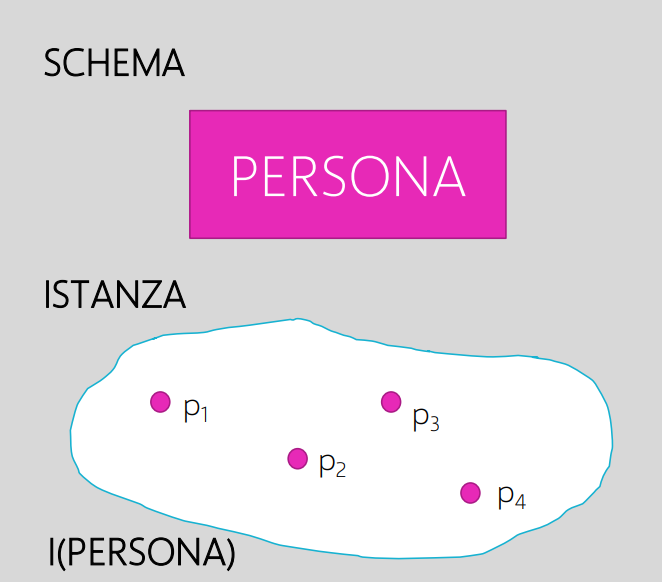
\includegraphics[width=0.5\linewidth]{image3.png}
        \caption{Esempio di Entita}
        \label{fig:placeholder}
    \end{figure}
\subsection{Relazione}
\begin{itemize}
    \item \textbf{Significato}: una relazione $R$ rappresenta un \textbf{legame logico} tra
    due o più entità.  
    Possono esistere relazioni:
    \begin{itemize}
        \item \textbf{binarie}, quando coinvolgono due entità diverse;
        \item \textbf{ternarie}, quando coinvolgono tre entità;
        \item \textbf{ennarie}, quando coinvolgono $n$ entità.  
    \end{itemize}
    \textbf{Caso particolare:} una relazione binaria può essere definita anche sulla stessa entità (detta \textbf{relazione ricorsiva}), ad esempio la relazione \emph{“impiegato-supervisore”} all’interno dell’entità \emph{Dipendente}.

    \item \textbf{Sintassi grafica}: una relazione $R$ si rappresenta nello schema
    con un \textbf{rombo} collegato, tramite linee spezzate, alle entità coinvolte nella
    relazione.  
    Il nome della relazione viene scritto all’interno o accanto al rombo.

    \item \textbf{Istanza}: data una relazione $R$ tra $n$ entità $E_1, E_2, \ldots, E_n$, 
    un’istanza della relazione è una \textbf{ennupla} di istanze delle entità coinvolte.  
    L’insieme di tutte le ennuple costituisce la \textbf{popolazione della relazione}.

    In altre parole, le ennuple rappresentano i \textbf{collegamenti concreti} tra le istanze delle entità.  
    Se immaginiamo la relazione come una tabella, ciascuna riga (ennupla) contiene i riferimenti alle istanze delle due entità collegate.  

    \textbf{Esempio:}  
    Sia $E =$ \emph{Studente} e $F =$ \emph{Corso}, e sia $R =$ \emph{Iscrizione}.  
    Un’istanza della relazione può essere l’ennupla $(\text{Mario Rossi}, \text{Analisi 1})$, 
    che rappresenta il fatto che lo studente “Mario Rossi” è iscritto al corso “Analisi 1”.  
    L’insieme di tutte le ennuple del tipo $(\text{Studente}, \text{Corso})$ forma la popolazione della relazione \emph{Iscrizione}.
    \item \textbf{Esempio} : Supponiamo di aver inserito nello schema le entità
\emph{PERSONA} e \emph{COMUNE}, e ipotizziamo che nei
requisiti sia indicata la necessità di gestire la
\emph{RESIDENZA} delle persone nei comuni italiani.
Rappresento con il costrutto relazione il concetto
di \emph{RESIDENZA}
\end{itemize}
\begin{figure}[!h]
    \centering
    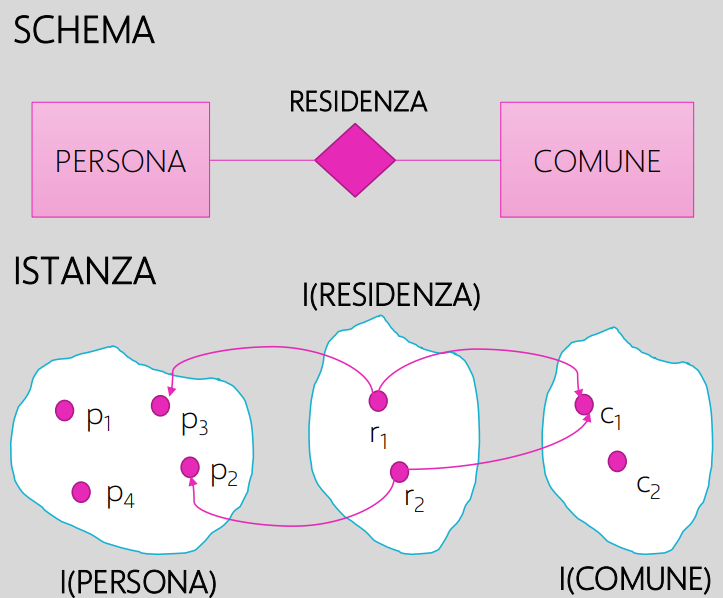
\includegraphics[width=0.5\linewidth]{image4.png}
    \caption{Esempio di Relazione}
    \label{fig:placeholder}
\end{figure}
\newpage
\subsubsection{Relazione Ricorsiva}
E’ una relazione binaria sulla stessa entità.
\begin{figure}[!h]
    \centering
    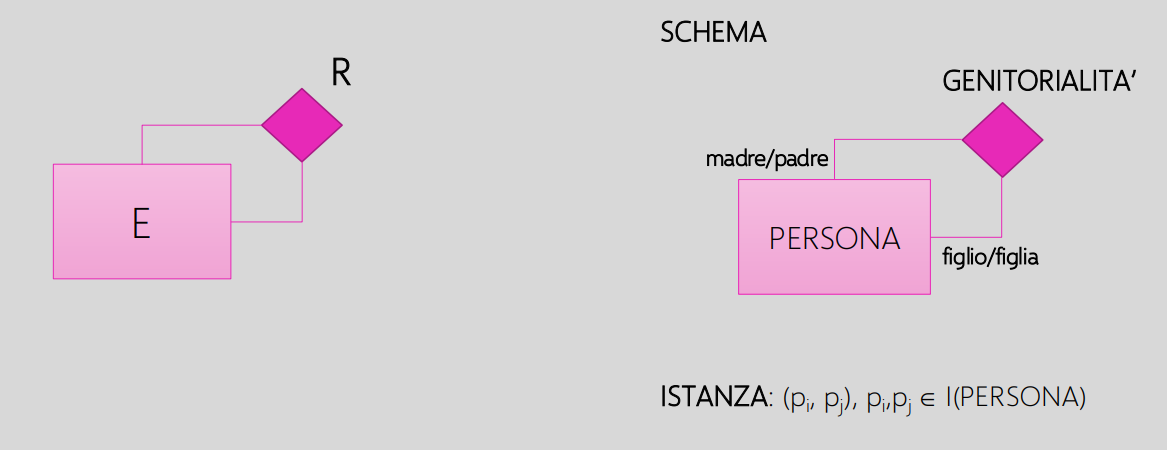
\includegraphics[width=0.7\linewidth]{image5.png}
    \caption{Relazione Ricorsiva}
    \label{fig:placeholder}
\end{figure}
\subsubsection{Relazione Ternaria}

Una \textbf{relazione ternaria} coinvolge tre entità e viene utilizzata quando un concetto del sistema informativo può essere rappresentato solo se sono presenti contemporaneamente tre istanze, una per ciascuna entità coinvolta.

\begin{itemize}
    \item Ogni istanza della relazione associa \textbf{una terna} di entità (E$_1$, E$_2$, E$_3$).  
    \item L’esistenza della relazione \textbf{richiede sempre} la presenza di tutte e tre le entità: non è possibile che ne manchi una.  
    \item Non esistono casi in cui la stessa terna debba essere rappresentata più volte.  
\end{itemize}

\begin{center}
    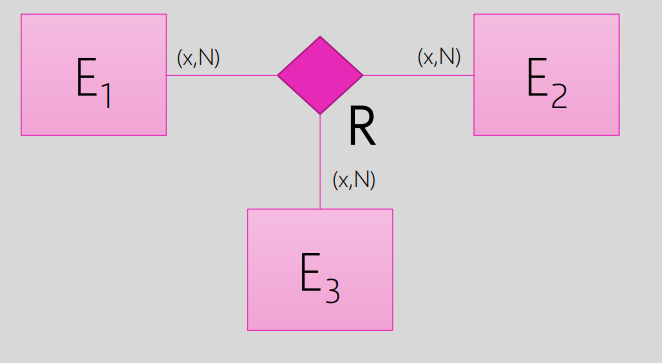
\includegraphics[width=0.55\linewidth]{image17.png}
    \label{fig:relazione_ternaria}
\end{center}

\subsubsection{Indizi di modellazione errata (uso improprio della relazione ternaria)}

In alcuni casi, l'utilizzo di una \textbf{relazione ternaria} può indicare una modellazione errata.  
Questo avviene quando una relazione tra tre entità non richiede realmente la presenza simultanea di tutte e tre le istanze.

\begin{itemize}
    \item Se per rappresentare lo stato del sistema informativo sarebbe sufficiente collegare \textbf{solo due entità per volta}, la relazione ternaria è superflua.  
    \item In tali casi, la relazione ternaria può essere sostituita da \textbf{tre relazioni binarie indipendenti}.
\end{itemize}



\noindent
\textbf{Esempio:}  
La relazione ternaria \emph{Partecipa(Medico, Paziente, Ospedale)} è errata se nel sistema esistono già le relazioni binarie:  
\emph{Lavora\_in(Medico, Ospedale)}, \emph{Visita(Medico, Paziente)} e \emph{Ricoverato\_in(Paziente, Ospedale)}.  
In questo caso, la relazione ternaria non aggiunge alcuna informazione nuova ed è quindi ridondante.
\noindent
Un ulteriore indizio di modellazione errata si verifica quando, in una relazione ternaria $R(A, B, C)$, si osserva il seguente comportamento:

\begin{itemize}
    \item Se una coppia $(a,b)$ compare in una terna $(a,b,c)$ istanza della relazione,  
    \item e una coppia $(b,c')$ compare in una terna $(a',b,c')$ istanza della relazione,
\end{itemize}

allora risultano automaticamente presenti anche le terne $(a,b,c')$ e $(a',b,c)$.

\noindent
Questo significa che le combinazioni tra le entità non dipendono realmente tutte e tre tra loro:  
la relazione ternaria può quindi essere scomposta in più relazioni binarie indipendenti senza perdita di informazione.
\noindent
\textbf{In sintesi:} se da due terne si possono dedurre automaticamente altre combinazioni tra le stesse entità,  
la relazione ternaria è ridondante e andrebbe sostituita da più relazioni binarie.

\begin{tcolorbox}[colback=yellow!15!white, colframe=orange!80!black, title=\textbf{Kristian semplifica in questo modo}]
Le \textbf{relazioni ternarie} vanno usate solo quando il significato della relazione dipende \textbf{strettamente da tutte e tre le entità coinvolte}.  

\begin{itemize}
    \item Se anche una sola entità può essere esclusa o rappresentata separatamente, allora la relazione non è veramente ternaria.  
    \item Nella maggior parte dei casi, è meglio sostituire una relazione ternaria con \textbf{più relazioni binarie indipendenti}.
\end{itemize}

\noindent
\textbf{In sintesi:}  
se puoi evitarla, \textbf{evitala}. Le relazioni ternarie rendono più difficile la progettazione e la traduzione nel modello relazionale.
\end{tcolorbox}
\subsubsection{Esempio coretto di relazione ternaria}
Vogliamo rappresentare il fatto che un prodotto venga fornito ad un dipartimento da un fornitore. Ogni
dipartimento può scegliere quali prodotti ordinare dai fornitori selezionando un sottoinsieme dei prodotti
forniti dal fornitore. Ogni fornitore vende a più dipartimenti prodotti diversi. Ogni prodotto viene venduto
da più fornitori.
\begin{figure}[!h]
    \centering
    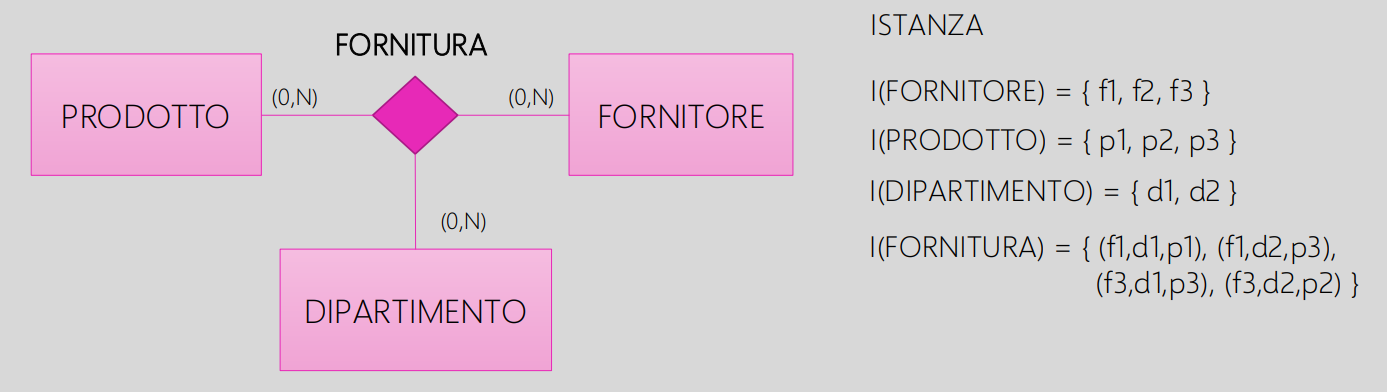
\includegraphics[width=0.75\linewidth]{image18.png}
    \caption{Esempio Relazione Ternaria}
    \label{fig:placeholder}
\end{figure}
\subsubsection{Come capire se un concetto ha vita propria}
Nel modello Entità-Relazione, per stabilire se un concetto debba essere rappresentato come 
\textbf{entità} o come \textbf{relazione}, è fondamentale chiedersi se tale concetto
\textit{ha una vita propria} all'interno del sistema informativo.

\begin{tcolorbox}[colback=yellow!15!white, colframe=black, title=Definizione]
Un concetto ha \textbf{vita propria} se può esistere in modo indipendente dalle altre entità,
cioè se ha senso considerarlo come un oggetto autonomo, anche quando non è collegato ad altri.
\end{tcolorbox}

\noindent
Per verificarlo, è possibile porsi alcune domande:

\begin{itemize}
  \item Può esistere anche senza essere collegato ad altre entità?
  \item Ha senso registrarlo nel sistema anche se non è associato ad altri elementi?
  \item Possiede attributi che descrivono sé stesso e non il legame con altri?
\end{itemize}

\noindent
Se la risposta è \textbf{sì} a queste domande, il concetto possiede vita propria e deve essere rappresentato come \textbf{entità}.
In caso contrario, se esiste solo come collegamento tra altre entità, è più corretto rappresentarlo come \textbf{relazione}.

\begin{center}
\begin{tabular}{|p{3.2cm}|p{5.3cm}|p{5.3cm}|}
\hline
\textbf{Caratteristica} & \textbf{Entità (ha vita propria)} & \textbf{Relazione (non ha vita propria)} \\
\hline
Esiste indipendentemente da altre & Può esistere da sola nel sistema & Esiste solo se collega altre entità \\
\hline
Ha senso da sola & Ha significato anche isolata & Ha senso solo nel contesto di un legame \\
\hline
Attributi & Descrivono l’oggetto in sé & Descrivono il legame tra entità \\
\hline
Esempio & Studente, Insegnamento, Docente & Sostiene, Frequenta, Acquista \\
\hline
\end{tabular}
\end{center}

\noindent
\textbf{Esempio applicativo:} nel caso della relazione \textit{ESAME}, se essa rappresenta l'atto con cui
uno studente sostiene un insegnamento (registrando solo \textit{data} e \textit{voto}),
non ha vita propria e va modellata come \textbf{relazione}.
Se invece si vogliono gestire appelli d’esame con \textit{aula}, \textit{docente} e \textit{orario}, 
esso assume significato autonomo e può essere rappresentato come \textbf{entità}.





\subsection{Attributo}
\begin{itemize}
    \item \textbf{Significato} :Rappresenta una proprietà elementare di un’entità (o
relazione).
Ogni attributo di entità (o relazione) associa ad ogni
istanza di entità (o relazione) UNO e UN SOL valore
appartenente ad un dominio (insieme di VALORI
AMMISSIBILI). 
    \item \textbf{Sintassi grafica} : collegato a una entità e a forma di pallino
\item \textbf{Esempio} : Rappresento con il costrutto entità il concetto di
PERSONA, ipotizzando che nei requisiti sia indicata
la necessità di gestire nella base di dati il nome e il
cognome di un gruppo di persone.
Aggiungo quindi il nome e il cognome come
attributi dell’entità PERSONA.
\begin{figure}[!h]
    \centering
    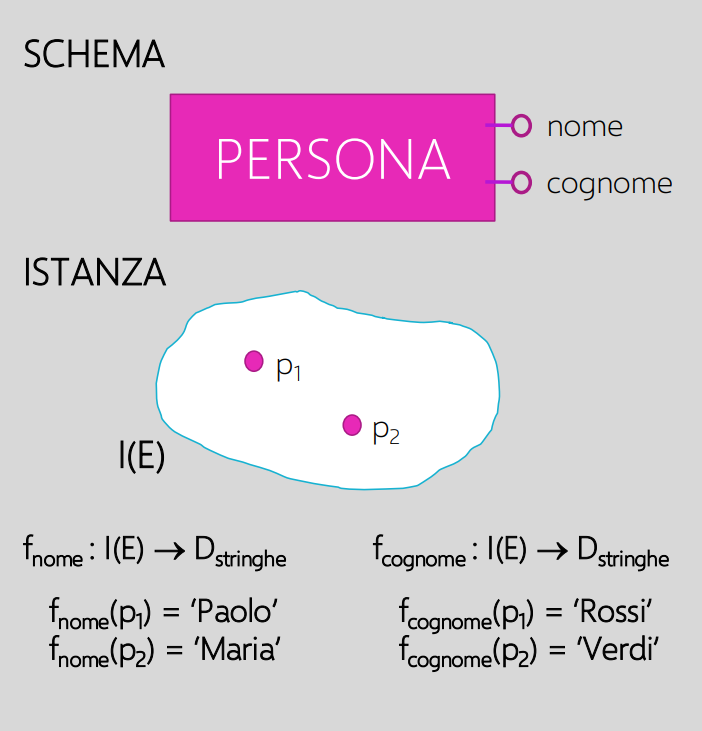
\includegraphics[width=0.5\linewidth]{image6.png}
    \caption{Esempio Attributo}
    \label{fig:placeholder}
\end{figure}
\subsubsection{Attributo opzionale e multivalore}  
Un \textbf{attributo opzionale} o \textbf{multivalore} deriva da un attributo normale, specificando un \textbf{vincolo di cardinalità} sui valori che esso può assumere.  
Il vincolo di cardinalità indica quante volte un attributo può comparire in corrispondenza di una stessa entità.  
Il valore predefinito è \textbf{(1,1)}, che significa “obbligatorio e singolo valore”.  

I principali casi sono:  
\begin{itemize}
    \item \textbf{(0,1)} : attributo opzionale → può essere assente o presente una sola volta;  
    \item \textbf{(1,N)} : attributo multivalore → deve essere presente almeno una volta e può comparire più volte;  
    \item \textbf{(0,N)} : attributo opzionale e multivalore → può essere assente o, se presente, avere più valori.
\end{itemize}

\begin{figure}[!h]
    \centering
    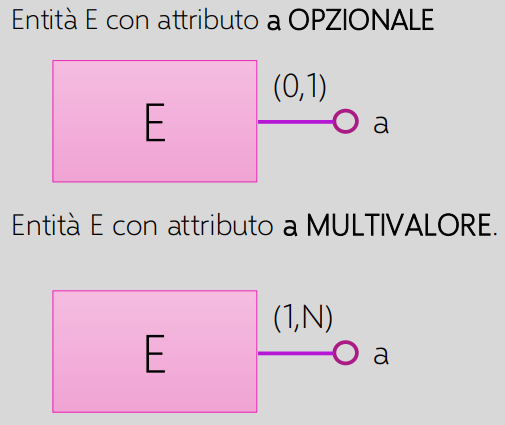
\includegraphics[width=0.5\linewidth]{image12.png}
    \caption{Attributo opzionale e/o multivalore}
    \label{fig:placeholder}
\end{figure}

\noindent
\textbf{Esempio pratico}  

Si consideri l’entità \emph{PERSONA}, per la quale si vogliono memorizzare:
\begin{itemize}
    \item \textbf{Codice fiscale}, \textbf{nome}, \textbf{cognome} e \textbf{data di nascita} — attributi obbligatori e a singolo valore;  
    \item \textbf{Patente di guida} — attributo \textbf{opzionale} \((0,1)\), poiché una persona può possederla o meno;  
    \item \textbf{Recapiti telefonici} — attributo \textbf{multivalore} \((1,N)\), poiché ogni persona può avere uno o più numeri di telefono (ad esempio cellulare, casa, lavoro).
\end{itemize}

\noindent


\begin{figure}[!h]
    \centering
    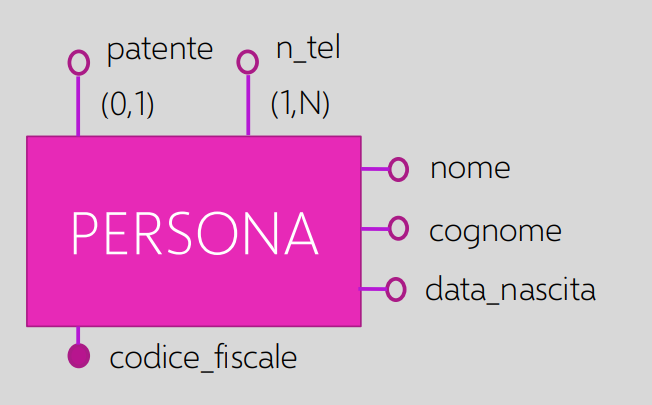
\includegraphics[width=0.5\linewidth]{image13.png}
    \caption{Esempio di attributo opzionale e multivalore per l’entità PERSONA}
    \label{fig:placeholder}
\end{figure}
\end{itemize}
\subsubsection{Attributo composto}
Un \textbf{attributo composto} consente di raggruppare più attributi di un’entità o di una relazione che presentano una stretta \textbf{affinità di significato}.  
In questo modo si possono rappresentare in modo più ordinato e logico informazioni che, pur essendo distinte, appartengono a un unico concetto complessivo.

\noindent
Ad esempio, per rappresentare l’entità \emph{PERSONA}, si possono gestire nella base di dati i seguenti attributi:  
\textbf{codice fiscale}, \textbf{nome}, \textbf{cognome}, \textbf{data di nascita} e \textbf{indirizzo}.  

\noindent
L’attributo \textbf{indirizzo} può essere considerato un attributo composto, poiché a sua volta può essere suddiviso nei sottoattributi:
\begin{itemize}
    \item \textbf{Città}
    \item \textbf{Via}
    \item \textbf{Numero civico}
\end{itemize}

\noindent
In un diagramma ER, l’attributo composto viene rappresentato con un’ellisse principale collegata a più ellissi minori, ognuna delle quali rappresenta un sottoattributo.

\begin{figure}[!h]
    \centering
    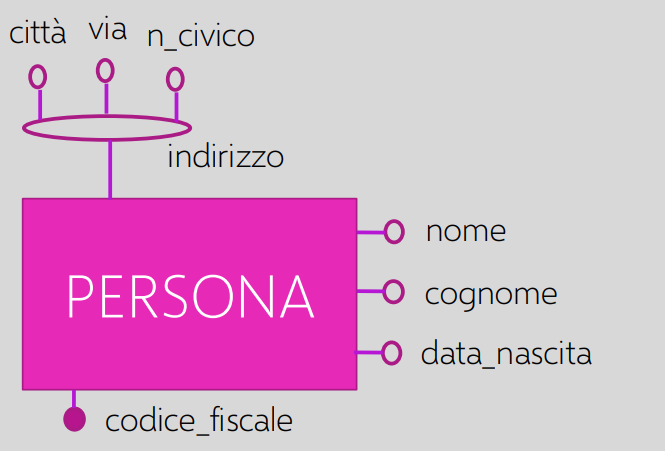
\includegraphics[width=0.5\linewidth]{image14.png}
    \caption{Esempio di attributo composto per l’entità PERSONA}
    \label{fig:placeholder}
\end{figure}


\subsection{Identificatore di Entità}
\begin{itemize}
    \item \textbf{Significato}:Data un’entità E, è un insieme di proprietà (attributi
e/o relazioni) che identificano univocamente le
istanze dell’entità.
Un insieme di proprietà \textbf{IDENTIFICA
UNIVOCAMENTE} le istanze di E se non esistono
due istanze di E che presentano gli stessi
valori/istanze nelle proprietà dell’insieme.
    \item \textbf{Sintassi grafica} : collegato a una entità e a forma di un pallino pieno, puo anche essere una linea che intercorre in due attributi sempre a fine con un pallino pieno
    \begin{figure}[!h]
        \centering
        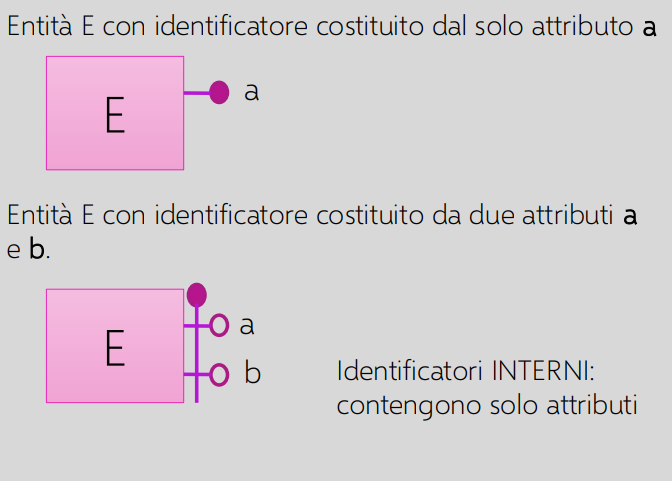
\includegraphics[width=0.5\linewidth]{image7.png}
        \caption{sintassi grafica: identificatori interni}
        \label{fig:placeholder}
    \end{figure}
    \begin{figure}[!h]
        \centering
        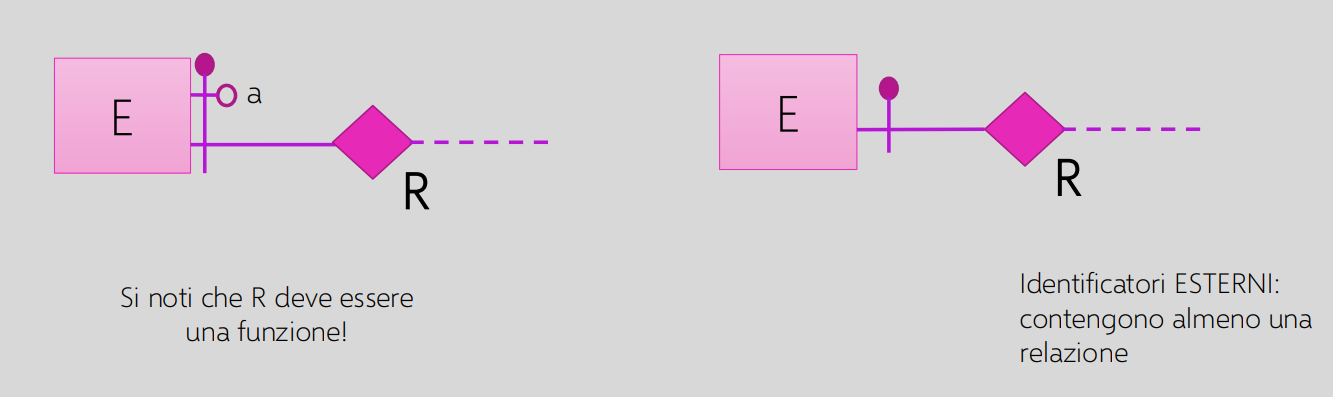
\includegraphics[width=0.75\linewidth]{image8.png}
        \caption{sintassi grafica: identificatori esterni}
        \label{fig:placeholder}
    \end{figure}
    \newpage
\item \textbf{Esempio}:
Rappresento con il costrutto entità il concetto di
\emph{PERSONA}, ipotizzando che nei requisiti sia indicata
la necessità di gestire nella base di dati, il codice
fiscale, il nome, il cognome e la data di nascita di un
gruppo di persone.
\begin{figure}[!h]
    \centering
    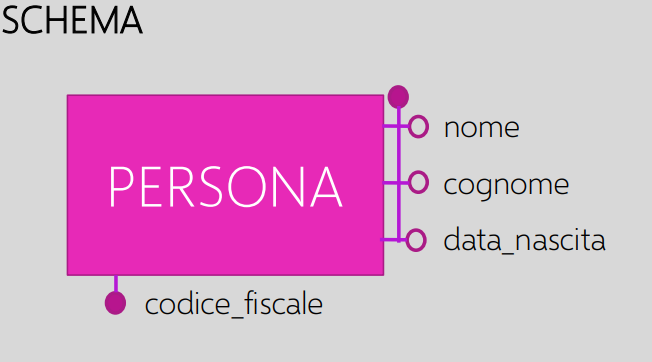
\includegraphics[width=0.5\linewidth]{image9.png}
    \label{fig:placeholder}
\end{figure}
\end{itemize}
La scelta dell’identificatore va sempre
fatta considerando proprietà
significative per il sistema informativo.
A livello concettuale l’introduzione di
nuovi attributi identificatori (ad
esempio l’ID) è da \textbf{evitare}.
\subsection{Generalizzazione}
La \textbf{generalizzazione} rappresenta un legame logico, analogo al concetto di \textbf{ereditarietà} nella programmazione a oggetti, tra un’entità padre e una o più entità figlie.  
Serve per modellare situazioni in cui più entità condividono alcune caratteristiche comuni, ma possiedono anche attributi o relazioni specifiche.

\begin{itemize}
    \item \textbf{Significato}:  
    È una relazione logica tra un’entità padre \emph{E} e $n$ entità figlie ($E_1, E_2, \ldots, E_n$), dove $E$ rappresenta una classe di oggetti più generale rispetto a quelle rappresentate dalle entità figlie.  
    Le entità figlie ereditano gli attributi e le relazioni dell’entità padre, aggiungendo eventualmente elementi propri.

    \item \textbf{Sintassi grafica}:  
    Le entità figlie coinvolte nella generalizzazione vengono collegate all’entità padre mediante una linea che converge in un triangolo (o freccia) rivolto verso l’entità padre.

    \begin{figure}[!h]
        \centering
        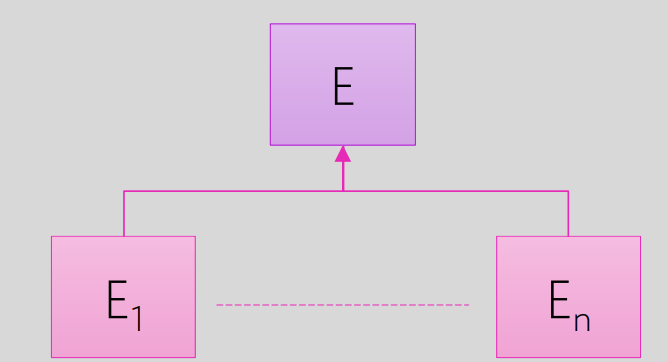
\includegraphics[width=0.5\linewidth]{image16.png}
        \caption{Sintassi grafica della generalizzazione}
        \label{fig:placeholder}
    \end{figure}

    \item \textbf{Esempio}:  
    Si consideri l’entità \emph{PERSONA}, per la quale nei requisiti è indicata la necessità di distinguere tra \emph{STUDENTE} e \emph{DOCENTE}.  
    In questo caso si può utilizzare una generalizzazione in cui:
    \begin{itemize}
        \item \textbf{PERSONA} è l’entità padre, che contiene gli attributi comuni (ad esempio: nome, cognome, data di nascita);
        \item \textbf{STUDENTE} e \textbf{DOCENTE} sono le entità figlie, che ereditano gli attributi di PERSONA e possono avere attributi propri (es. matricola per STUDENTE, dipartimento per DOCENTE).
    \end{itemize}

    \begin{figure}[!h]
        \centering
        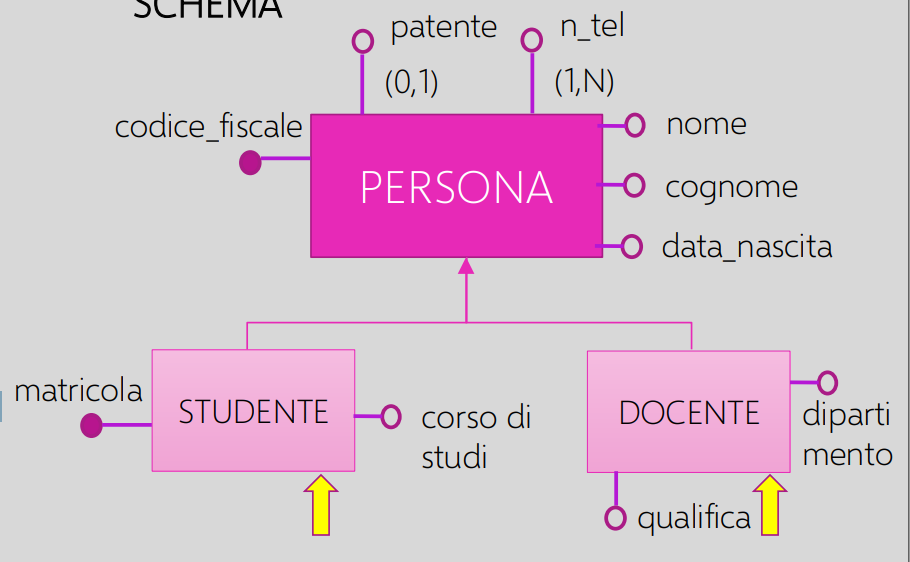
\includegraphics[width=0.5\linewidth]{image15.png}
        \caption{Esempio di generalizzazione tra PERSONA, STUDENTE e DOCENTE}
        \label{fig:placeholder}
    \end{figure}
\end{itemize}



\begin{tcolorbox}[colback=yellow!15!white, colframe=orange!80!black, title=\textbf{Proprietà}]
Le \textbf{proprietà delle istanze di entità} che partecipano a una \textbf{generalizzazione} sono le seguenti:

\begin{itemize}
    \item Ogni istanza di un’entità figlia $E_i$ è anche un’istanza dell’entità padre $E$.
    \item Ogni proprietà (attributi, identificatori e relazioni) dell’entità padre $E$ è condivisa da tutte le entità figlie $E_1, E_2, \ldots, E_n$.
\end{itemize}

\noindent
In altre parole, le entità figlie \textbf{ereditano} tutte le caratteristiche dell’entità padre, e possono aggiungerne di proprie.
\end{tcolorbox}
\subsubsection{Classificazione delle Generalizzazioni}
Nel modello \textbf{Entità–Relazione}, una generalizzazione può assumere diverse forme, a seconda del tipo di legame tra l’entità padre (superclasse) e le entità figlie (sottoclassi).  
Le combinazioni derivano dall’incrocio di due caratteristiche fondamentali:  
\begin{itemize}
    \item il grado di \textbf{copertura} (Totale o Parziale);  
    \item il grado di \textbf{esclusività} (Esclusiva o Sovrapposta).  
\end{itemize}

\noindent
Ecco i principali tipi di gerarchia nel modello ER:

\begin{enumerate}
    \item \textbf{Totale ed Esclusiva (t,e)}:  
    ogni istanza della superclasse appartiene \textbf{obbligatoriamente} a una e una sola sottoclasse.  
    \emph{Esempio:} l’entità \emph{VEICOLO} è generalizzata in \emph{MOTO} e \emph{AUTO}.  
    Ogni veicolo deve essere o moto o auto, ma non può essere entrambi.

    \item \textbf{Totale e Sovrapposta (t,s)}:  
    ogni istanza della superclasse deve appartenere ad almeno una sottoclasse, ma può appartenere a \textbf{più sottoclassi} contemporaneamente.  
    \emph{Esempio:} l’entità \emph{PERSONA} è generalizzata in \emph{STUDENTE} e \emph{LAVORATORE}.  
    Una persona può essere sia studente sia lavoratore.

    \item \textbf{Parziale ed Esclusiva (p,e)}:  
    non tutte le istanze della superclasse devono appartenere a una sottoclasse; se appartengono, ne hanno solo una.  
    \emph{Esempio:} l’entità \emph{ANIMALE} è generalizzata in \emph{DOMESTICO} e \emph{SELVATICO}.  
    Un animale può essere domestico, selvatico o nessuno dei due, ma non entrambi.

    \item \textbf{Parziale e Sovrapposta (p,s)}:  
    non tutte le istanze devono appartenere a una sottoclasse; chi appartiene può essere in più sottoclassi.  
    \emph{Esempio:} l’entità \emph{PERSONA} è generalizzata in \emph{SPORTIVO} e \emph{ARTISTA}.  
    Una persona può essere sportiva, artista, entrambe o nessuna delle due.
\end{enumerate}

\begin{tcolorbox}[colback=yellow!15!white, colframe=orange!80!black, title=\textbf{Kristian semplifica in questo modo}]
Le \textbf{gerarchie di generalizzazione} si classificano in base a due proprietà fondamentali:

\begin{itemize}
    \item \textbf{Totale} → ogni istanza della superclasse deve appartenere ad almeno una sottoclasse.  
    \item \textbf{Parziale} → alcune istanze della superclasse possono non appartenere a nessuna sottoclasse.  
    \item \textbf{Esclusiva (o Disgiunta)} → un’istanza può appartenere solo a una sottoclasse.  
    \item \textbf{Sovrapposta} → un’istanza può appartenere a più sottoclassi contemporaneamente.
\end{itemize}

\noindent
In sintesi:  
\textbf{Totale/Parziale} indica \emph{se tutte le istanze partecipano},  
mentre \textbf{Esclusiva/Sovrapposta} indica \emph{come partecipano}.
\end{tcolorbox}

	\include{vincolidiCardinalita}   % NB: nessuno spazio nel nome file!
	\section{Strategie per la progettazione concettuale}

Lo sviluppo di uno \textbf{schema concettuale} può essere considerato a tutti gli effetti un \textbf{processo di ingegnerizzazione}, in quanto richiede un insieme di fasi metodiche e ragionate per trasformare le specifiche di un problema reale in una rappresentazione astratta ma coerente e precisa.  

In altre parole, progettare uno schema concettuale non significa solo disegnare entità e relazioni, ma \textbf{analizzare, organizzare e strutturare le informazioni} in modo sistematico, seguendo principi simili a quelli utilizzati nell’ingegneria del software.

\begin{tcolorbox}[colback=yellow!20,colframe=yellow!50!black,title={\textbf{Nota Bene}},boxrule=0.8pt,arc=2mm]
Per \textbf{ingegnerizzazione} si intende l’\textit{applicazione di un metodo rigoroso e pianificato} alla progettazione, allo sviluppo e alla verifica di un sistema complesso.  
Nel contesto della modellazione dei dati, ciò significa:  
\begin{itemize}
  \item partire da requisiti chiari e ben definiti;
  \item progettare in modo graduale e controllato (Top-Down, Bottom-Up o Inside-Out);
  \item assicurarsi che lo schema finale sia corretto, completo e privo di ambiguità.
\end{itemize}
\end{tcolorbox}

\begin{center}
\textit{Ricorda che uno schema concettuale è una rappresentazione astratta e indipendente dal linguaggio di implementazione, che descrive le informazioni e le relazioni fondamentali di un sistema informativo.}
\end{center}

% -------------------------------------------------
\subsection{Strategia Top-Down}

La strategia \textbf{Top-Down} consiste nel partire da una \textbf{visione globale del sistema} e procedere verso una \textbf{maggiore specificazione dei dettagli}.  
È un approccio deduttivo: si comincia con concetti generali e astratti per poi raffinarli gradualmente fino a ottenere uno schema concettuale completo e preciso.

\begin{itemize}
  \item \textbf{Fase 1:} considerare le specifiche globalmente e produrre uno schema iniziale \textbf{completo ma con pochi concetti astratti}.  
  \item \textbf{Fase 2:} \textbf{raffinare} progressivamente i concetti astratti fino ad arrivare a uno schema concettuale \textbf{dettagliato in ogni parte}.
\end{itemize}

\begin{tcolorbox}[colback=yellow!20,colframe=yellow!50!black,title={\textbf{Nota Bene}},boxrule=0.8pt,arc=2mm]
La strategia Top-Down è particolarmente utile quando si ha una visione chiara e globale del dominio applicativo.  
Permette di mantenere coerenza tra le parti del progetto, ma richiede una buona capacità di astrazione e pianificazione.
\end{tcolorbox}

\begin{center}
\textit{Esempio:} prima si individuano le entità principali (\textit{Studente}, \textit{Corso}, \textit{Docente}), poi si aggiungono relazioni e attributi specifici come \textit{data di nascita}, \textit{esame sostenuto}, \textit{voto}, ecc.
\end{center}

% -------------------------------------------------
\subsection{Strategia Bottom-Up}

La strategia \textbf{Bottom-Up} adotta un approccio opposto rispetto al Top-Down.  
In questo caso si parte dai \textbf{dettagli elementari} per poi integrarli progressivamente fino a ottenere la visione complessiva del sistema.  
È un metodo \textbf{induttivo}, ideale quando si dispone di molte informazioni di base ma non ancora di una struttura generale.

\begin{itemize}
  \item \textbf{Fase 1:} \textbf{decomporre} le specifiche iniziali in \textbf{parti elementari}, ovvero piccole frasi o porzioni di testo che descrivono uno stesso concetto o una singola informazione.  
  \item \textbf{Fase 2:} \textbf{generare gli schemi} per ciascuna parte elementare individuata.  
  \item \textbf{Fase 3:} \textbf{fondere gli schemi} parziali introducendo, se necessario, altri costrutti del modello E-R, in modo da \textbf{integrare} tutti gli elementi e ottenere lo \textbf{schema finale}.
\end{itemize}

\begin{tcolorbox}[colback=yellow!20,colframe=yellow!50!black,title={\textbf{Nota Bene}},boxrule=0.8pt,arc=2mm]
La strategia Bottom-Up è utile quando le specifiche non sono complete o sono distribuite in frammenti separati.  
Permette di costruire lo schema passo dopo passo, ma richiede attenzione nella fase di integrazione per evitare ridondanze o incoerenze tra i diversi schemi parziali.
\end{tcolorbox}

\begin{center}
\textit{Esempio:} si analizzano prima frasi come “uno studente sostiene un esame” o “un docente insegna un corso”, si crea uno schema per ciascuna, e infine si uniscono tutti in un unico schema concettuale completo.
\end{center}

% -------------------------------------------------
\subsection{Strategia Inside-Out}

La strategia \textbf{Inside-Out} rappresenta un approccio intermedio rispetto a Top-Down e Bottom-Up.  
Si parte da alcuni \textbf{concetti centrali o fondamentali} del dominio, detti \textbf{concetti guida}, e si costruisce lo schema espandendolo progressivamente verso l’esterno.

\begin{itemize}
  \item \textbf{Fase 1:} \textbf{individuare} nelle specifiche alcuni concetti importanti, detti \textbf{concetti guida}.  
  \item \textbf{Fase 2:} \textbf{generare gli schemi} relativi ai concetti guida scelti.  
  \item \textbf{Fase 3:} \textbf{fondere gli schemi} precedenti e aggiungere gradualmente gli altri concetti fino a ottenere lo \textbf{schema concettuale completo}.
\end{itemize}

\begin{tcolorbox}[colback=yellow!20,colframe=yellow!50!black,title={\textbf{Nota Bene}},boxrule=0.8pt,arc=2mm]
La strategia Inside-Out è utile quando si riescono a identificare con chiarezza alcuni elementi chiave del sistema.  
Permette di concentrarsi inizialmente sulle parti più rilevanti e poi di estendere lo schema, garantendo coerenza e controllo durante l’espansione.
\end{tcolorbox}

\begin{center}
\textit{Esempio:} si parte dai concetti guida come \textit{Studente} e \textit{Corso}, si definiscono le loro relazioni principali, e poi si estende lo schema aggiungendo altri concetti come \textit{Esame}, \textit{Docente} o \textit{Dipartimento}.
\end{center}

% -------------------------------------------------
\subsection{Analisi di qualità dello schema}

L’\textbf{analisi di qualità} di uno schema concettuale serve a valutare se il modello prodotto rappresenta correttamente e in modo efficace il dominio di interesse.  
Essa comprende quattro aspetti fondamentali:
\begin{itemize}
  \item Verifica di correttezza
  \item Verifica di completezza
  \item Verifica di minimalità
  \item Verifica di leggibilità
\end{itemize}

\textbf{Verifica di correttezza}  
Uno schema concettuale è \textbf{corretto} se utilizza propriamente i costrutti del modello concettuale adottato (nel nostro caso, il modello E-R).  
La correttezza si valuta controllando che lo schema rispetti le regole sintattiche e semantiche del modello.

\begin{itemize}
  \item \textbf{Errori sintattici:} utilizzo scorretto dei costrutti del modello E-R, senza rispettarne le regole formali.  
  \textit{Esempi:}
  \begin{itemize}
    \item introduzione di una generalizzazione di relazioni;
    \item relazioni non collegate ad alcuna entità;
    \item relazioni che possiedono un identificatore.
  \end{itemize}
  
  \item \textbf{Errori semantici (errori d’uso):} uso improprio dei costrutti del modello, senza rispettarne il significato.  
  \textit{Esempi:}
  \begin{itemize}
    \item uso di una relazione per rappresentare un concetto che dovrebbe essere un’entità autonoma;
    \item uso di un attributo per rappresentare un concetto complesso o collegato ad altri concetti in più punti dello schema.
  \end{itemize}
\end{itemize}

\textbf{Verifica di completezza e minimalità}  
Uno schema concettuale è \textbf{completo} se rappresenta tutte le informazioni di interesse e consente di eseguire tutte le operazioni previste dalle specifiche.  
È invece \textbf{minimale} quando tutti i concetti presenti nei requisiti sono rappresentati una sola volta, evitando ridondanze o duplicazioni.

\textbf{Verifica di leggibilità}  
La leggibilità riguarda la \textbf{chiarezza e l’organizzazione visiva} dello schema.  
Uno schema ben leggibile deve essere ordinato, coerente e facilmente interpretabile anche da chi non lo ha progettato.

\begin{tcolorbox}[colback=yellow!20,colframe=yellow!50!black,title={\textbf{Nota Bene}},boxrule=0.8pt,arc=2mm]
Un buon schema concettuale deve essere:
\begin{itemize}
  \item \textbf{Corretto} → rispetta le regole sintattiche e semantiche del modello E-R;
  \item \textbf{Completo} → include tutte le informazioni richieste;
  \item \textbf{Minimale} → evita ridondanze e duplicazioni;
  \item \textbf{Leggibile} → chiaro, ordinato e facilmente comprensibile.
\end{itemize}
Solo quando tutte queste condizioni sono soddisfatte, lo schema può essere considerato di \textbf{alta qualità}.
\end{tcolorbox}

% -------------------------------------------------
\subsection{Ridondanze}

Uno \textbf{schema concettuale non minimale} può contenere delle \textbf{ridondanze}, ossia rappresentazioni multiple dello stesso concetto logico.  
I casi più comuni di ridondanza sono:

\begin{itemize}
    \item \textbf{Ereditarietà delle relazioni}
    \item \textbf{Cicli di relazioni}
\end{itemize}

\begin{figure}[!h]
    \centering
    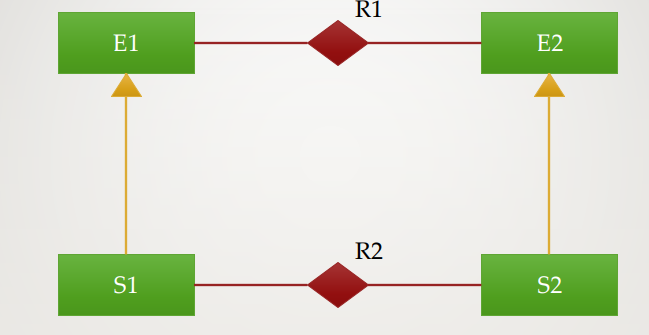
\includegraphics[width=0.55\linewidth]{image19.png}
    \caption{Ereditarietà delle relazioni}
    \label{fig:ereditarieta-relazioni}
\end{figure}

\begin{center}
È \textbf{probabile, ma non certo}, che la relazione \textit{R2} sia ridondante.  
Va quindi verificato se \textit{R2} rappresenti lo stesso legame logico già espresso da \textit{R1}; se così fosse, \textit{R2} deve essere eliminata in quanto effettivamente ridondante.
\end{center}

\begin{figure}[!h]
    \centering
    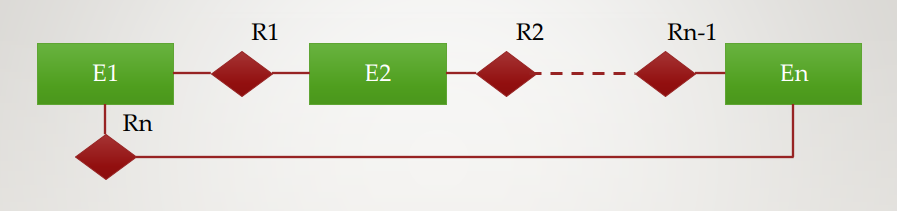
\includegraphics[width=0.75\linewidth]{image20.png}
    \caption{Ciclo di relazioni}
    \label{fig:ciclo-relazioni}
\end{figure}

\begin{center}
È \textbf{probabile, ma non certo}, che una delle relazioni $R_i$ sia ridondante.  
Va quindi verificato se la relazione $R_i$ possa essere ottenuta \textbf{dalla composizione delle altre relazioni}.  
Se così fosse, $R_i$ deve essere eliminata in quanto effettivamente ridondante.
\end{center}

% -------------------------------------------------
\subsection{Semplificazioni dello schema}

Non sempre le \textbf{relazioni ternarie} sono facili da leggere e interpretare; per questo motivo, la loro eliminazione può talvolta migliorare la \textbf{leggibilità dello schema concettuale}.  

Le seguenti operazioni possono essere applicate per semplificare o trasformare una relazione ternaria:

\begin{itemize}
  \item \textbf{Trasformazione di una relazione ternaria in un’entità}  
  Questa operazione è \textbf{sempre applicabile} e consiste nel sostituire la relazione ternaria con una nuova entità, collegata tramite relazioni binarie alle entità originarie.  

  \item \textbf{Riduzione di una relazione ternaria a due relazioni binarie}  
  Questa operazione è possibile solo se una delle entità coinvolte partecipa alla relazione ternaria con \textbf{cardinalità (1,1)}.  
  In tal caso, la relazione ternaria può essere sostituita da due relazioni binarie equivalenti, mantenendo il significato logico dello schema.
\end{itemize}

\begin{tcolorbox}[colback=yellow!20,colframe=yellow!50!black,title={\textbf{Nota Bene}},boxrule=0.8pt,arc=2mm]
La trasformazione o riduzione delle relazioni ternarie deve essere eseguita con attenzione:  
l’obiettivo è migliorare la leggibilità dello schema senza alterarne il significato semantico.
\end{tcolorbox}

\begin{figure}[!h]
    \centering
    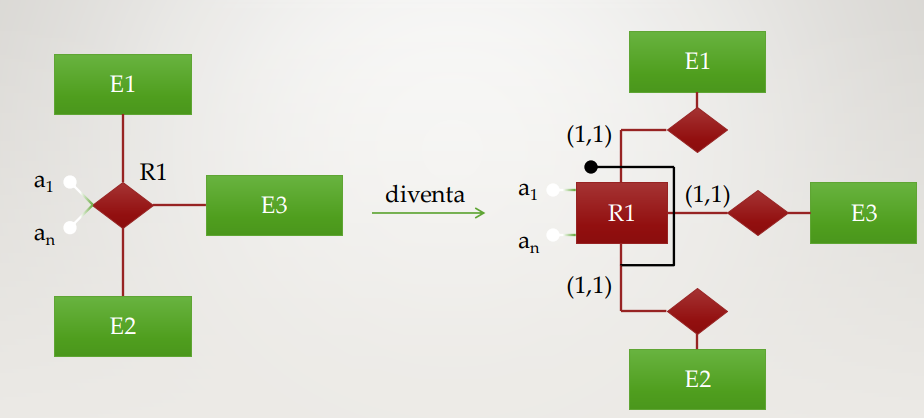
\includegraphics[width=0.75\linewidth]{image21.png}
    \caption{Trasformazione di una relazione ternaria in un’entità}
    \label{fig:relazione-ternaria-entita}
\end{figure}

\begin{figure}[H]
    \centering
    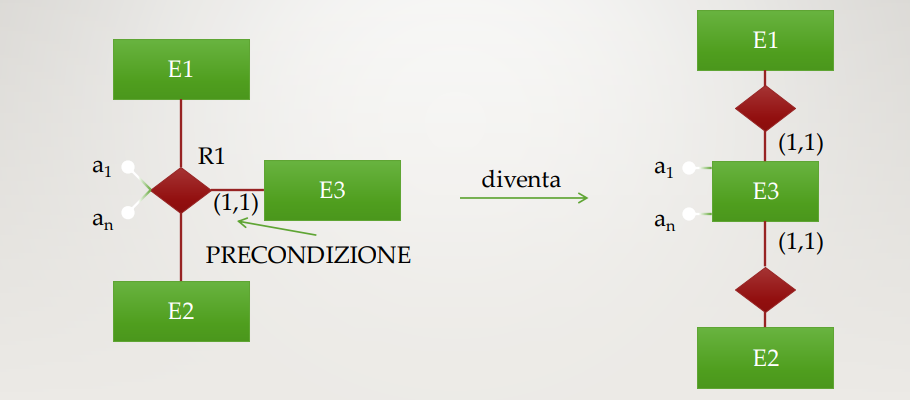
\includegraphics[width=0.75\linewidth]{image22.png}
    \caption{Riduzione di una relazione ternaria a due relazioni binarie}
    \label{fig:relazione-ternaria-binarie}
\end{figure}
Un ulteriore miglioramento nella leggibilità si ottiene esplicitando, nelle \textbf{generalizzazioni sovrapposte}, l’entità che rappresenta la sovrapposizione.  
In questo modo, la generalizzazione sovrapposta viene trasformata in una \textbf{generalizzazione esclusiva}, rendendo lo schema più chiaro e facilmente interpretabile.


	\section{Modello Relazionale}

Nel corso del tempo si sono sviluppati diversi modelli per la rappresentazione e l’organizzazione dei dati all’interno dei sistemi informativi. Tra i principali ricordiamo:

\begin{itemize}
    \item \textbf{Modello gerarchico/reticolare} (anni 1960–1970): tra i primi modelli di gestione dei dati, organizzati in forma gerarchica o a rete.
    \item \textbf{Modello relazionale} (anni 1980–oggi): introdotto da Edgar F. Codd, rappresenta i dati mediante tabelle (relazioni) e costituisce la base dei moderni DBMS relazionali.
    \item \textbf{Modello ad oggetti} (anni 1990–2000): integra i concetti di programmazione orientata agli oggetti con la gestione dei dati.
    \item \textbf{Modello a oggetti/relazionale (object–relational)} (anni 2000–oggi): un’evoluzione del modello relazionale che consente l’integrazione di tipi complessi, eredità e relazioni tra oggetti. Esempio: SQL3.
    \item \textbf{Modello a grafo – RDF (Resource Description Framework)} (anni 2005–oggi): rappresenta i dati sotto forma di grafo orientato, utile nel contesto del web semantico. Esempio: Neo4j.
    \item \textbf{Modelli noSQL} (document-based, column-based, key–value, ecc.) (anni 2010–oggi): nati per la gestione di grandi volumi di dati non strutturati e per garantire maggiore scalabilità. Esempio: MongoDB.
\end{itemize}
\subsection{Costrutti Principali del Modello Relazionale}
Il modello relazionale costituisce la base dei moderni database e si fonda su alcuni \textbf{costrutti principali}:

\begin{itemize}
    \item \textbf{Domini di base}: rappresentano l’insieme dei valori ammissibili per ciascun attributo.
    \item \textbf{Relazione (o tabella)}:
    \begin{itemize}
        \item Definizione come insieme di \textbf{n–uple} (righe).
        \item Ogni n–upla rappresenta un record all’interno della relazione.
    \end{itemize}
    \item \textbf{Superchiavi, Chiavi e Chiavi primarie}: identificano univocamente le tuple all’interno di una relazione.
    \item \textbf{Vincoli di integrità referenziale}: garantiscono la coerenza dei riferimenti tra tabelle.
    \item \textbf{Vincoli di integrità generici}: assicurano la validità logica dei dati rispetto a condizioni predefinite.
\end{itemize}
\subsection{Domini di Base}
Sono i domini da cui si scelgono i valori delle proprietà delle
istanze di informazione da rappresentare. I domini tipici sono:
\begin{itemize}
    \item Caratteri
    \item Stringhe
    \item Numeri
    \item Numeri decimali a virgola fissa
    \item Numeri decimali a virgola mobile
    \item Dominio del Tempo
\end{itemize}
\subsection{Costrutto Relazionale}
Una relazione può essere vista come una tabella ad esempio:

\begin{table}[H]
    \centering
    \renewcommand{\arraystretch}{1.2} % aumenta leggermente l'altezza delle righe
    \begin{tabular}{l c r}
        \hline
        \textbf{Città} & \textbf{CAP} & \textbf{Abitanti} \\
        \hline
        Milano  & 20100 & 1\,300\,000 \\
        Verona  & 37100 & 350\,000 \\
        Brescia & 25100 & 250\,000 \\
        \hline
    \end{tabular}
    \caption{Esempio di relazione \textbf{Città} con attributi \textit{(Nome, CAP, Abitanti)}}
    \label{tab:citta}
\end{table}
Una tabella è un contenitore di dati la cui struttura è caratterizzata da una lista di collonne:
\begin{itemize}
    \item I dati sono scritti nelle righe dove ogni riga descrive le
caratteristiche di un’istanza dell’informazione da rappresentare
    \item I valori contenuti nelle colonne descrivono sempre la stessa
proprietà delle istanze di informazione da rappresentare.
\end{itemize}
\subsubsection{Definizione: Relazione come insieme di ennuple (LISTS)}

Dati $n$ insiemi di valori (detti \textbf{domini}) $D_1, \ldots, D_n$ con $n > 0$, si indica con 
$D_1 \times \ldots \times D_n$ il loro \textbf{prodotto cartesiano}:

\[
D_1 \times \ldots \times D_n = 
\{ (v_1, \ldots, v_n) \mid v_1 \in D_1, \ldots, v_n \in D_n \}
\]

Una \textbf{relazione} $\rho$ di grado $n$ è un qualsiasi \textbf{sottoinsieme} di 
$D_1 \times \ldots \times D_n$:

\[
\rho \subseteq D_1 \times \ldots \times D_n
\]

dove $(v_1, \ldots, v_n)$ è una \textbf{ennupla} della relazione e 
$|\rho|$ rappresenta la \textbf{cardinalità} della relazione 
(ovvero il numero di ennuple presenti).
Si noti che i domini $D_1 ,\ldots,D_n$ possono essere a \textbf{cardinalità infinita}, mentre le relazioni sono SEMPRE a \textbf{cardinalità finita}.
Possiamo dire che
\begin{itemize}
    \item Non è definito alcun ordinamento sulle ennuple di una relazione
    \item Non sono ammessi DUPLICATI di una ennupla
    \item Nella definizione di relazione come insieme di ennuple, i valori nelle ennuple sono ordinati
\end{itemize}
\begin{figure}[H]
    \centering
    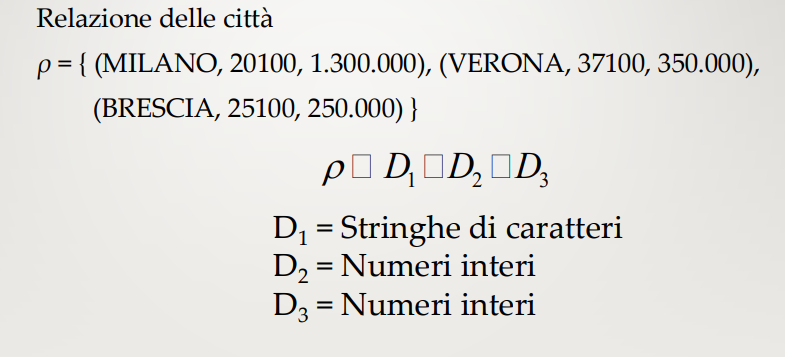
\includegraphics[width=0.75\linewidth]{image23.png}
    \caption{Esempio di relazione con insieme di ennuple}
\end{figure}
\paragraph{Accesso ai valori di una ennupla:}
Se $t$ e una ennupla $(V_1,\ldots,V_n)$ il valore posto in i-esima posizione si indica con la notazione $t[i]$. Questa modalità di accesso ai valori non è efficace per l'uso pratico delle relazioni.
Si preferisce quindi assegnare un nome alle colonne;ciò conduce all'introduzione della definizione come insieme di \textbf{TUPLE}.
\subsubsection{Definizione  RELAZIONE come insieme di tuple (MAPPINGS)}
Sia $X$ un insieme di nomi e si $\Delta$ l'insieme di tutti i domini di base ammessi dal modello.
Si definisce la funzione:\\
$DOM:X \to \Delta $\\

Tale funzione associa ad ogni nome A di X un dominio $DOM(A)$ di $\Delta$.I nomi di X si dicono \textbf{attributi}.
\begin{figure}[H]
    \centering
    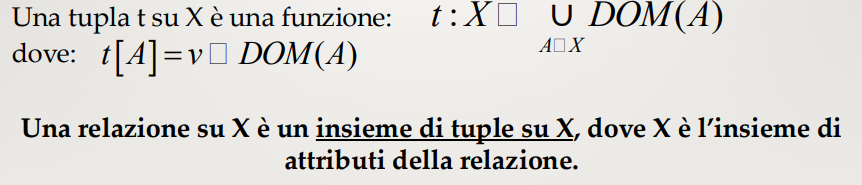
\includegraphics[width=0.75\linewidth]{image24.png}
\end{figure}
\begin{figure}[H]
    \centering
    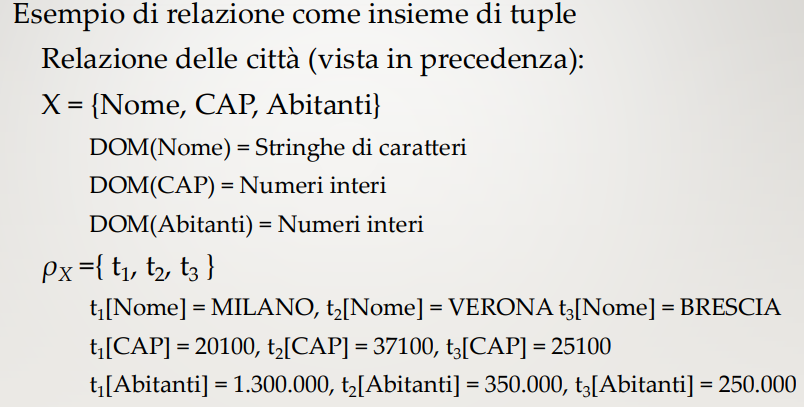
\includegraphics[width=0.75\linewidth]{image25.png}
    \caption{Esempio}
\end{figure}
\begin{itemize}
    \item Una relazione è un insieme di tuple e quindi non può contenere tuple duplicate
    \item I domini per gli attirbuti possono essere solo domini di base, non sono ammessi altri domini, ne il prodotto cartesiano di domini
    \item In generale una base di dati relazionale è costitutia da piu relazioni.
\end{itemize}
\subsection{Come progettare una basi di dati relazionale}
Nel modello relazionale lo schema è costituito da un insieme di relazioni o tabelle.
Lo strumento formale che serve per definire dipendenze tra attributi nel modello relazionale è costituito dalle \textbf{ dipendenze funzionali}.

\paragraph{Per Esempio:}
Vogliamo rappresentare in una base di dati relazionale le informazioni sulla proprietà degli appartamenti siti nel comune di Verona.
\begin{itemize}
    \item Per ogni appartamento volgiamo memorizzare : il codice ecografico (univoco), la categoria catastale e l'indirizzo composto da : via,numero civico, subalterno
    \item Per ogni proprietario si registra: il codice fiscale, il nome, il cognome e la data di nascita.
    \item Un appartamento può essere in comproprietà e un proprietario può possedere più appartamenti.
\end{itemize}
\begin{figure}[H]
    \centering
    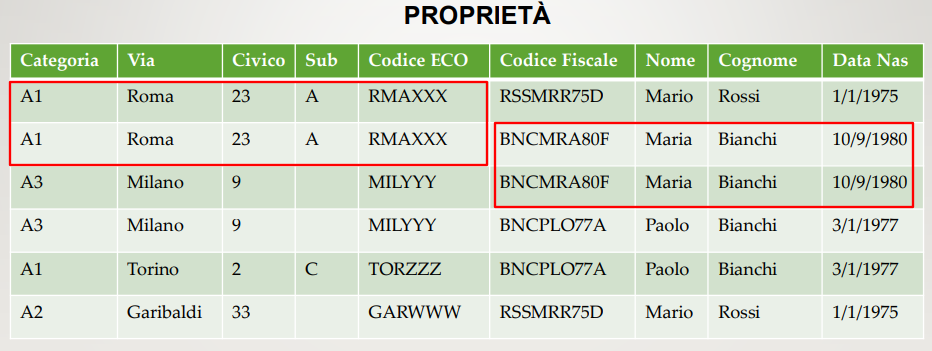
\includegraphics[width=0.75\linewidth]{image26.png}
    \caption{Schema relazionale con solo una relazione}
\end{figure}
Nella relazione unica ogni riga rappresenta un contratto di proprietà e richiede di precisare tutti i dati di un appartamento e tutti i dati di un proprietario.
Ciò implica che:
\begin{itemize}
    \item Non è possibile rappresentare un appartamento che non abbia un proprietario, né rappresentare un proprietario senza appartamento,
    \item I dati di un appartamento vengono replicati per ogni proprietario
    \item I dati di un proprietario vengono replicati per ogni appartamento di proprietà.
\end{itemize}
\paragraph{Anomalie:} La presenza di ridondanza inutile nella base di dati provoca le seguenti anomalie:
\begin{itemize}
    \item \textbf{ANOMALIE DI AGGIORNAMENTO} : per aggiornare il valore di un attributo si è obbligati a modificare tale valore su più tuple.
    \item  \textbf{ANOMALIE DI INSERIMENTO} : per inserire una nuova tupla è necessario inserire valori al momento sconosciuti (sostituibili da valori nulli) per gli attributi non disponibili.
    \item \textbf{ANOMALIE DI CANCELLAZIONE} : per cancellare una tupla è necessario cancellare valori ancora validi oppure inserire valori nulli per gli attributi da cancellare.
\end{itemize}
E possibile ridurre la ridondanza nei dati decomponendo la relazione. Sono possibili diverse decomposizioni.
\begin{figure}[H]
    \centering
    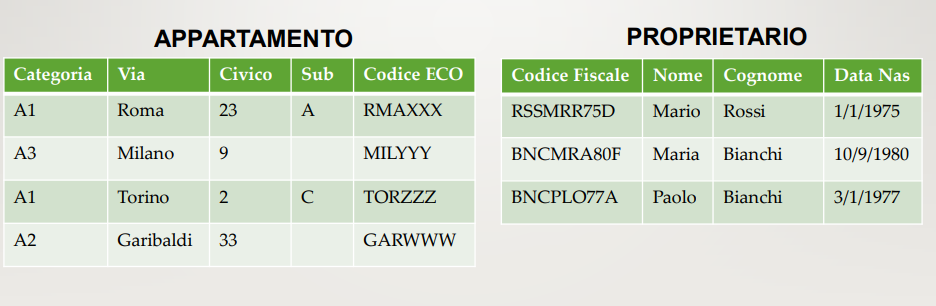
\includegraphics[width=0.75\linewidth]{image27.png}
    \caption{Decomposizione 1}
\end{figure}
\begin{figure}[H]
    \centering
    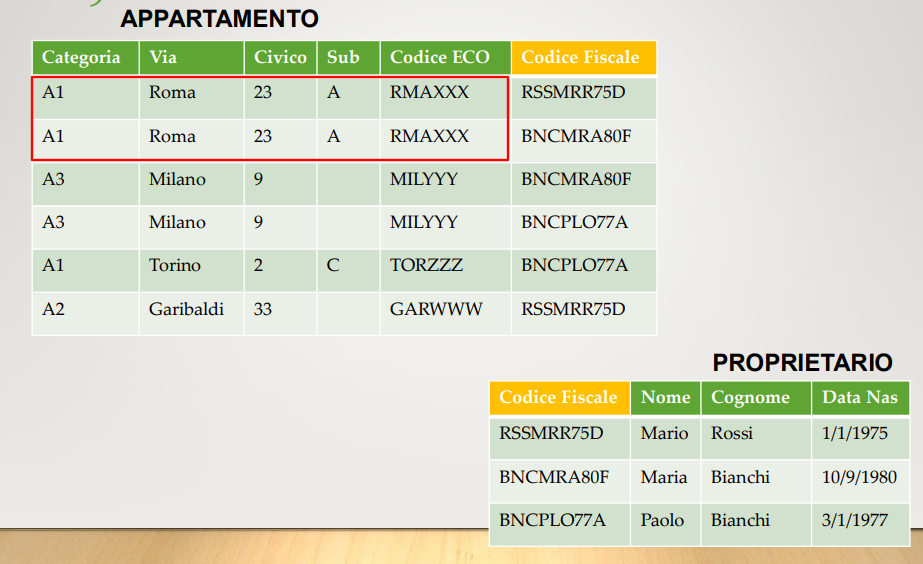
\includegraphics[width=0.75\linewidth]{image28.png}
    \caption{Decomposizione 2}
    \label{fig:placeholder}
\end{figure}
\begin{figure}[H]
    \centering
    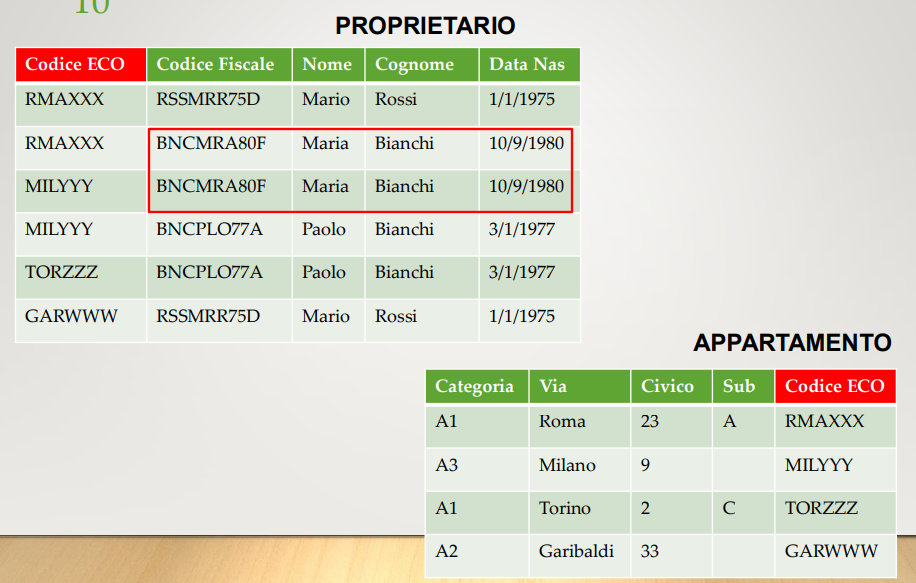
\includegraphics[width=0.75\linewidth]{image29.png}
    \caption{Decomposizione 3}
\end{figure}
\begin{figure}[H]
    \centering
    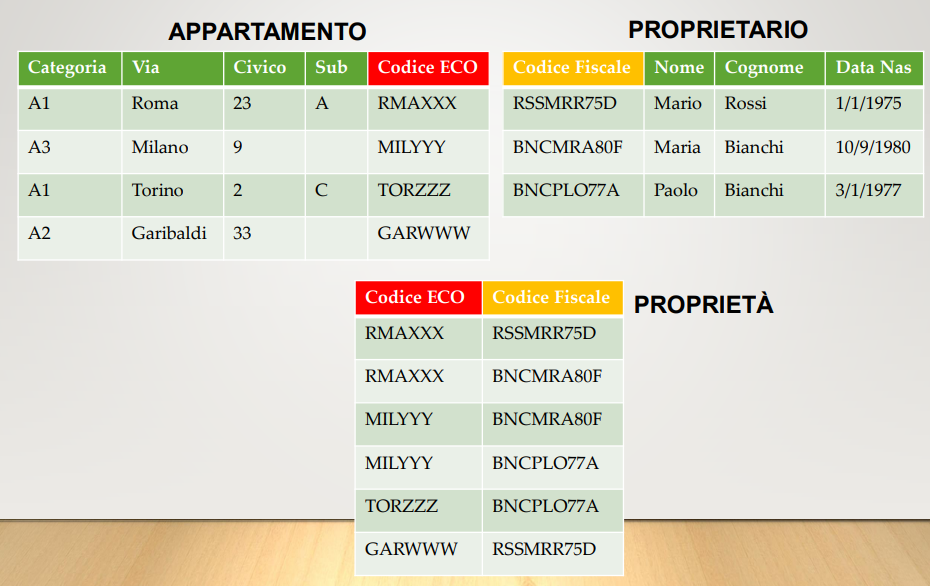
\includegraphics[width=0.75\linewidth]{image30.png}
    \caption{Decomposizione 4}
\end{figure}
Si noti che i legami tra relazioni si realizzano attraverso la replicazione di un insieme di attributi, dove il legame tra due tuple si intende stabilito quando esse presentano gli stessi valori negli attributi replicati.
Il modello relazionale è \textbf{value-based} (basato su valori).
Il modello non prevede l'uso di puntatori per rappresentare legami tra i dati.
Essere value-based implica:
\begin{itemize}
    \item Completa indipendenza dall'implementazione e dallo schema fisico
    \item Facilità di trasferimento dei dati tra sistemi
    \item Viene rappresentato solo ciò che è rilevante per il sistema informativo
\end{itemize}
\subsubsection{Terminologia di schema di una relazione}
E costituito dal nome della relazione e da un insieme di nomi per i suoi attributi:\\
$R(X)$ oppure $R(A_1,\dots,A_n)$ oppure $R(A_1:D_1,\dots,A_n:D_n)$
\subsubsection{Terminologia Schema di una base di dati}
E costituito da un insieme di schemi di relazioni:\\
$S = \{R_1(X_1),\dots,R_n(X_n)\}$ con $R_1 \neq R_2 \neq \dots R_n$
\subsubsection{Terminologia istanza di una relazione di schema $R(X)$}
E un insieme r di tuple su X dove $r = \{ t_1,\dots,t_k \}$
\subsubsection{Terminologia istanza di una base di dati di schema $S = \{R_1(X_1),\dots,R_n(X_n)$}
E costituito da un insieme di istanze delle relazioni $R_1(X_1),\dots,R_n(X_n): db = \{r_1,\dots,r_n\}$
\subsection{Valori nulli}

Secondo la definizione formale di \textit{relazione}, ogni tupla dovrebbe contenere per ciascun attributo un valore appartenente al relativo dominio.  
Nelle basi di dati reali, però, questa condizione non è sempre rispettabile: può accadere che un attributo non abbia un valore disponibile.  

I motivi principali per cui un valore può mancare sono i seguenti:

\begin{itemize}
    \item \textbf{Valore inesistente}  
    L'attributo $A$ è concettualmente opzionale: per quella specifica istanza non esiste alcun valore significativo da inserire.  
    \textit{Esempio:} il campo ``secondo numero di telefono'' per un cliente che possiede un solo numero.

    \item \textbf{Valore sconosciuto}  
    Il valore dell'attributo $A$ esiste, ma non è attualmente noto alla base di dati.  
    \textit{Esempio:} l'indirizzo e-mail di un utente appena registrato che non lo ha ancora comunicato.

    \item \textbf{Valore sconosciuto o inesistente}  
    Non è possibile stabilire se l'informazione manchi perché non esiste o perché non è ancora conosciuta, oppure si preferisce rappresentare entrambe le situazioni allo stesso modo.  
    \textit{Esempio:} il campo ``data di scadenza del contratto'', che potrebbe non essere ancora stata definita oppure semplicemente non comunicata.
\end{itemize}
Per gestire queste situazioni si introduce il \textbf{valore nullo}.  
In questo modo il valore di un attributo in una tupla può essere:
\begin{itemize}
    \item un valore appartenente al dominio dell'attributo;
    \item il \texttt{NULL}, utilizzato per rappresentare un'informazione assente (inesistente o sconosciuta).
\end{itemize}

\textit{Esempio:} nel campo ``numero di telefono fisso'' di una tabella dei clienti, un cliente che non possiede un telefono fisso avrà come valore \texttt{NULL}.
\begin{figure}[H]
    \centering
    
\includegraphics[width=0.75\linewidth]{image31.png}
    \caption{Tupla su X con valori nulli}
\end{figure}
Si noti che:

\begin{itemize}
    \item \textbf{La presenza di valori nulli è ammessa solo in alcuni attributi.}  
    Non è infatti possibile avere tuple composte esclusivamente da valori nulli, poiché non rappresenterebbero alcuna informazione utile.

    \item \textbf{I valori nulli possono creare problemi negli attributi usati per rappresentare legami tra tuple.}  
    In particolare, negli attributi che fungono da chiave esterna, un valore \texttt{NULL} potrebbe rendere impossibile stabilire la relazione con altre tuple.
\end{itemize}

\textit{Esempio:}  
Si consideri una tabella \texttt{Prenotazioni} con l'attributo \texttt{idCliente} come chiave esterna verso la tabella \texttt{Clienti}.  
Se \texttt{idCliente} fosse \texttt{NULL}, non sarebbe possibile sapere quale cliente ha effettuato la prenotazione, rendendo l'informazione inutilizzabile.
\subsection{Vincoli di integrità}
Spesso è necessario introdurre dei \textbf{vincoli} (restrizioni) sull'istanza
di una base di dati, poiché non tutte le configurazioni possibili sono
compatibili con il sistema informativo che si vuole rappresentare.

Per specificare quali istanze sono considerate corrette si introduce il
concetto di \textbf{vincolo di integrità}.

\begin{tcolorbox}[
colback=yellow!20,
colframe=yellow!50!black,
title=\textbf{Vincolo di Integrità}
]
Un \textbf{vincolo di integrità} è una condizione (espressa come un predicato)
che deve essere sempre verificata da ogni istanza della base di dati.  
I vincoli di integrità assicurano che i dati memorizzati siano consistenti,
coerenti e validi rispetto al modello del sistema informativo.
\end{tcolorbox}
\subsection{Esempi di vincoli}

Siano date le seguenti relazioni:

\begin{itemize}
    \item \texttt{TRENO(Numero, OraPart, MinutoPart, Categoria, Destinazione, OraArr, MinutoArr)}
    \item \texttt{FERMATA(NumTreno, Stazione, OraFer, MinutoFer)}
\end{itemize}

I seguenti predicati esprimono possibili \textbf{vincoli di integrità} sulla relazione \texttt{TRENO}:

\[
\forall t \in TRENO :\; t[\text{OraPart}] \in \{0,1,\ldots,23\}
\]

\[
\forall t \in TRENO :\; t[\text{MinutoPart}] \in \{0,1,\ldots,59\}
\]

\[
\forall t \in TRENO :\; t[\text{Numero}] > 0
\]

\[
\forall t \in TRENO :\; t[\text{Numero}] > 5000 \;\Rightarrow\; t[\text{Categoria}] = \text{'regionale'}
\]
\[
\forall t, t' \in TRENO :\; t \neq t' \;\Rightarrow\; t[\text{Numero}] \neq t'[\text{Numero}]
\]
\textit{(Vincolo di unicità sul Numero del treno)}

\[
\forall f \in FERMATA :\; \exists t \in TRENO :\; t[\text{Numero}] = f[\text{NumTreno}]
\]
\textit{(Vincolo di chiave esterna: ogni fermata deve riferirsi a un treno esistente)}

\[
\forall t \in TRENO :\; t[\text{Categoria}] = \text{'regionale'}
\Rightarrow \exists f \in FERMATA :\; f[\text{NumTreno}] = t[\text{Numero}]
\]
\textit{(Se un treno è regionale allora deve avere almeno una fermata)}
\subsection{Classificazione vincoli di integrità}
Si distinguono inoltre alcuni vincoli particolari che rivestono un ruolo 
fondamentale, poiché assicurano proprietà generali valide per tutti gli 
schemi relazionali. Tali vincoli sono detti \textbf{vincoli strutturali}.

Essi comprendono:

\begin{itemize}
    \item \textbf{Vincoli di dominio}  
    Specificano quali valori possono essere assegnati a ciascun attributo 
    (esempio: l’attributo \texttt{OraPart} deve essere compreso tra 0 e 23).

    \item \textbf{Vincoli di tupla}  
    Impongono condizioni che devono essere verificate all'interno di una 
    singola tupla (esempio: \texttt{Numero} > 0).

    \item \textbf{Vincoli intrarelazionali}  
I vincoli intrarelazionali impongono condizioni sul contenuto di una
relazione e richiedono che ogni tupla soddisfi una certa proprietà
rispetto alle altre tuple della stessa relazione.

Una categoria particolarmente rilevante di tali vincoli è costituita
dai \textbf{vincoli di chiave}, che comprendono:
\begin{itemize}
    \item \textbf{Superchiave}: Data una relazione di schema $R(X)$, un insieme di attributi $K \subseteq X$
è una \textbf{superchiave} per $R(X)$ se, per ogni istanza $r$ di $R(X)$,
vale la seguente condizione:

\[
\forall t, t' \in r : t \neq t' \;\Rightarrow\; t[K] \neq t'[K]
\]

dove:

\[
t[K] \neq t'[K] \;\equiv\; \exists A_i \in K : t[A_i] \neq t'[A_i]
\]

    \item \textbf{Chiave candidata} : Data una relazione di schema $R(X)$, un insieme di attributi $K$, 
sottoinsieme di $X$, è \textbf{chiave candidata} (o \textbf{chiave}) per $R(X)$
se $K$ è superchiave per $R(X)$ e vale la seguente condizione:

\[
\neg \exists K' \subset K : K' \text{ è superchiave per } R(X)
\]
    \item \textbf{Chiave primaria} : Data una relazione di schema $R(X)$, la sua \textbf{chiave primaria}
è la chiave candidata scelta per \textit{identificare le tuple della relazione}.

Una chiave primaria $K$ ha le seguenti caratteristiche:

\begin{itemize}
    \item Non contiene \underline{mai valori nulli}.
    \item Su $K$ il sistema genera una struttura d’accesso ai dati (o indice)
          per supportare le interrogazioni.
\end{itemize}
\begin{tcolorbox}[colback=yellow!20, colframe=yellow!50!black, title={Kristian semplifica così – Le tre chiavi spiegate intuitivamente}]

\textbf{Superchiave}  
Una superchiave è \textbf{qualsiasi insieme di attributi che distingue sempre le tuple}.  
Se due tuple sono diverse, almeno un attributo della superchiave è diverso.

\textbf{Esempio:}  
Nella tabella STUDENTI(\underline{Matricola}, Nome, Cognome, Email)  
- Insiemi come \{Matricola\}, \{Matricola, Nome\}, \{Email, Cognome\} sono tutte superchiavi.  
Perché? Perché non esistono due studenti con la stessa combinazione di quei valori.

\vspace{0.4cm}

\textbf{Chiave candidata}  
Una chiave candidata è una \textbf{superchiave minimale}:  
non puoi togliere nessun attributo senza perdere l’unicità.

\textbf{Esempio:}  
- \{Matricola\} è chiave candidata perché basta da sola.  
- \{Email\} è un’altra chiave candidata.  
- Ma \{Matricola, Nome\} \textbf{non} è candidata: contiene attributi inutili, è troppo “larga”.

\vspace{0.4cm}

\textbf{Chiave primaria}  
È la \textbf{chiave candidata scelta} per identificare ufficialmente le tuple.  
Non può contenere NULL e il DB crea un indice su di essa.

\textbf{Esempio:}  
Se in STUDENTI scegliamo la chiave candidata \{Matricola\}, quella diventa la chiave primaria.  
Serve per identificare uno studente, fare ricerche, creare collegamenti con altre tabelle.

\end{tcolorbox}

\end{itemize}

 
    \item \textbf{Vincoli interrelazionali}  
    I vincoli interrelazionali impongono una restrizione al contenuto di una relazione
e specificano una condizione che ogni tupla della relazione deve soddisfare
rispetto alle tuple di altre relazioni della base di dati.Una sottocategoria importante di tali vincoli è costituita dai:
    \begin{itemize}
        \item \textbf{Vincoli di integrità referenziale}  
impone che ogni valore di una
\textit{chiave esterna} (foreign key) presente in una relazione
debba necessariamente comparire come valore di \textit{chiave primaria}
(primary key) nella relazione a cui fa riferimento.
%
In questo modo si garantisce la coerenza dei dati tra più tabelle
e si impedisce l'inserimento di tuple ``orfane'' non collegate a dati esistenti.

\begin{tcolorbox}[
colback=yellow!15!white,
colframe=orange!80!black,
title=\textbf{Kristian semplifica in questo modo}
]
Il vincolo di integrità referenziale è una regola che assicura che due tabelle
rimangano sempre coerenti tra loro.

\textbf{Significa:} se in una tabella inserisco una \textit{chiave esterna},
quel valore deve esistere come \textit{chiave primaria} nella tabella collegata.

\textbf{Esempio intuitivo:}

\begin{itemize}
    \item Tabella \texttt{Studenti(id, nome)}
    \item Tabella \texttt{Esami(idStudente, voto)}
\end{itemize}

Nella tabella \texttt{Esami}, il campo \texttt{idStudente} è una \textbf{foreign key}:
può contenere solo valori che esistono come \texttt{id} nella tabella \texttt{Studenti}.

Se provo a inserire un esame per lo studente \texttt{id = 50}, ma nella tabella
\texttt{Studenti} non esiste lo studente 50, il database blocca l'inserimento
perché violerei il vincolo di integrità referenziale.
\end{tcolorbox}
    \end{itemize}
\end{itemize}
\subsection{Notazione per indicare i vincoli strutturali}

\subsubsection{Chiave primaria}

La chiave primaria di una relazione $R(X)$ viene indicata
\textbf{sottolineando gli attributi} che la compongono.

Supponiamo che, per la tabella \texttt{TRENO}, venga scelto come chiave primaria
l'attributo \texttt{Numero}.  
La notazione per indicare tale chiave è:

\[
\texttt{TRENO(}\underline{\texttt{Numero}}\texttt{, OraPart, MinutoPart, Categoria, Destinazione, OraArr, MinutoArr)}
\]

Per la tabella \texttt{FERMATA}, la chiave primaria è composta dagli attributi
\texttt{NumTreno}, \texttt{Stazione}, \texttt{OraFer} e \texttt{MinutoFer}.
Si indica così:

\[
\texttt{FERMATA(}\underline{\texttt{NumTreno, Stazione}}\texttt{, OraFer, MinutoFer)}
\]

\bigskip

\subsubsection{Vincolo di integrità referenziale}

Un \textbf{vincolo di integrità referenziale} viene indicato
\textbf{riquadrando gli attributi soggetti al vincolo}
(nella tabella figlia)  
e collegandoli con una freccia al riquadro degli attributi
della tabella da cui la chiave primaria proviene (tabella padre).

Supponiamo che nella tabella \texttt{FERMATA} l'attributo
\texttt{NumTreno} sia una chiave esterna che fa riferimento
alla chiave primaria \texttt{Numero} della tabella \texttt{TRENO}.

La notazione diventa:

\[
\boxed{\texttt{Numero}} \quad \longleftarrow \quad
\texttt{TRENO(}\underline{\texttt{Numero}}\texttt{, OraPart, MinutoPart, Categoria, Destinazione, OraArr, MinutoArr)}
\]

\vspace{0.3cm}

\[
\boxed{\texttt{NumTreno}} \quad
\texttt{FERMATA(}\underline{\texttt{NumTreno, Stazione}}\texttt{, OraFer, MinutoFer)}
\]

\bigskip

\begin{tcolorbox}[
colback=yellow!15!white,
colframe=orange!80!black,
title=\textbf{Kristian semplifica in questo modo}
]
\textbf{Chiave primaria}: sottolineo gli attributi che identificano univocamente
le tuple della tabella.

\textbf{Chiave esterna (integrità referenziale)}: metto un riquadro attorno
all'attributo nella tabella ``figlia'' e lo collego con una freccia
alla chiave primaria della tabella ``padre''.

In questo modo si vede subito da dove arriva il valore e quale tabella controlla
la sua validità.
\end{tcolorbox}
\subsection{Esercizio}
\begin{figure}[H]
    \centering
    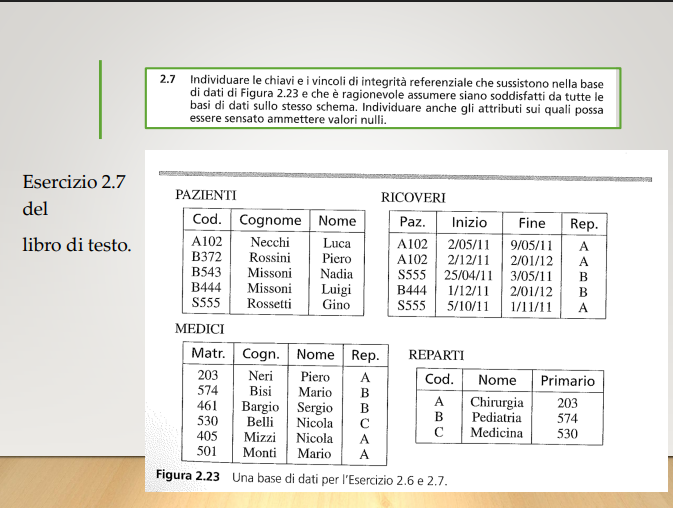
\includegraphics[width=1\linewidth]{image32.png}
    \label{fig:placeholder}
\end{figure}
\begin{figure}[H]
    \centering
    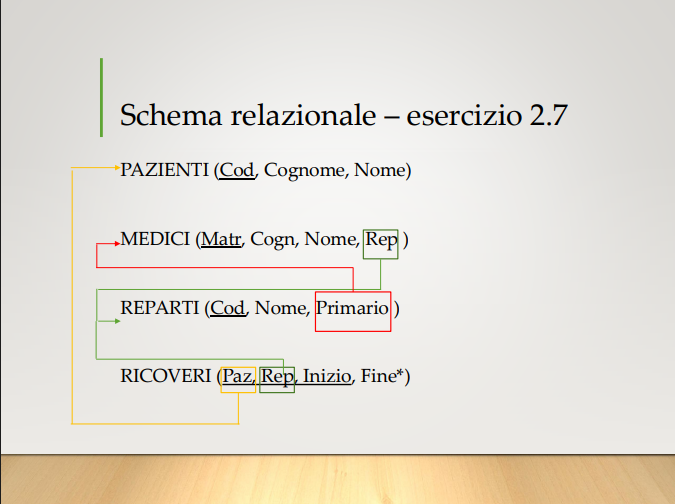
\includegraphics[width=1\linewidth]{image33.png}
    \caption{Soluzione}
    \label{fig:placeholder}
\end{figure}
\subsection{Progettazione Logica}

L’obiettivo della progettazione logica è quello di produrre uno \textbf{schema logico} che rappresenti in modo corretto, completo ed efficace tutte le informazioni contenute nello \textbf{schema concettuale}.

Prima della traduzione può essere necessario \textbf{ristrutturare lo schema ER} per i seguenti motivi:
\begin{itemize}
    \item \textbf{Semplificare} la fase di traduzione verso il modello logico.
    \item \textbf{Ottimizzare} le strutture in base al \textit{carico di lavoro} previsto (operazioni e query più frequenti).
\end{itemize}

Le principali fasi della \textbf{ristrutturazione dello schema ER} sono:
\begin{itemize}
    \item Analisi delle \textbf{ridondanze} dovute alla presenza di dati derivabili.
    \item \textbf{Eliminazione delle generalizzazioni} tramite le diverse strategie di trasformazione.
    \item \textbf{Accorpamento} o \textbf{partizionamento} di entità e relazioni, quando necessario.
    \item Scelta degli \textbf{identificatori principali} più adatti ed efficienti.
\end{itemize}

\subsubsection{Analisi della derivabilità}

L’analisi della derivabilità serve a individuare \textbf{dati che possono essere ricavati (derivati) da altri dati già presenti nello schema}.  
Questi dati non vanno memorizzati perché occupano spazio inutilmente e possono creare inconsistenze.

Esempi di dati derivabili:
\begin{itemize}
    \item \textbf{Attributi calcolabili} a partire da altri attributi della stessa entità  
    (es. ``età'' derivabile dalla ``data di nascita'').
    
    \item \textbf{Attributi derivabili} da informazioni presenti in entità diverse  
    (es. ``numero totale degli ordini di un cliente'' ricavabile dalla relazione \textit{Ordini}).
    
    \item \textbf{Attributi ottenuti con un conteggio}  
    (es. ``numero di iscritti a un corso'' ricavabile contando le partecipazioni).
    
    \item \textbf{Relazioni derivabili} dalla combinazione di altre relazioni  
    (es. una relazione ``LavoraIn'' può essere derivata combinando ``Impiegato'' e ``Dipartimento'' tramite una relazione intermedia).
\end{itemize}
\subsubsection{Analisi delle ridondanze}

In questa fase vengono analizzati i \textbf{dati derivabili} per decidere se conviene:
\begin{itemize}
    \item \textbf{Memorizzare il dato derivabile}, quando il costo del calcolo è \emph{maggiore} del costo di aggiornamento.
    \item \textbf{Non memorizzarlo e calcolarlo quando serve}, quando il costo del calcolo è \emph{minore} del costo di aggiornamento.
\end{itemize}

Il \textbf{costo} viene misurato in termini di numero di accessi per unità di tempo, valutando:
\begin{itemize}
    \item la frequenza con cui il dato deve essere calcolato,
    \item la frequenza con cui il dato dovrebbe essere aggiornato.
\end{itemize}
\subsubsection{Eliminazione delle Generalizzazioni}

Nel modello relazionale le generalizzazioni non sono direttamente rappresentabili.  
Per questo motivo esistono tre possibili strategie per trasformarle:
\begin{itemize}
    \item \textbf{Accorpamento delle entità figlie nel padre}.
    \item \textbf{Accorpamento dell’entità padre nelle entità figlie}.
    \item \textbf{Sostituzione della generalizzazione con relazioni}.
\end{itemize}

\subsubsection{Accorpamento delle entità figlie nel padre} 
Questa soluzione prevede:
\begin{itemize}
    \item Eliminazione delle entità figlie.
    \item Trasferimento nel padre di tutti gli attributi specifici delle entità figlie, trattandoli come \textbf{attributi opzionali}.
    \item Accorpamento nel padre di tutte le relazioni che coinvolgevano le entità figlie, impostando la \textbf{cardinalità minima a 0} dal lato del padre.
    \item Aggiunta di un attributo \textbf{TIPO} per distinguere le occorrenze corrispondenti alle ex entità figlie.
\end{itemize}
\begin{figure}[H]
    \centering
    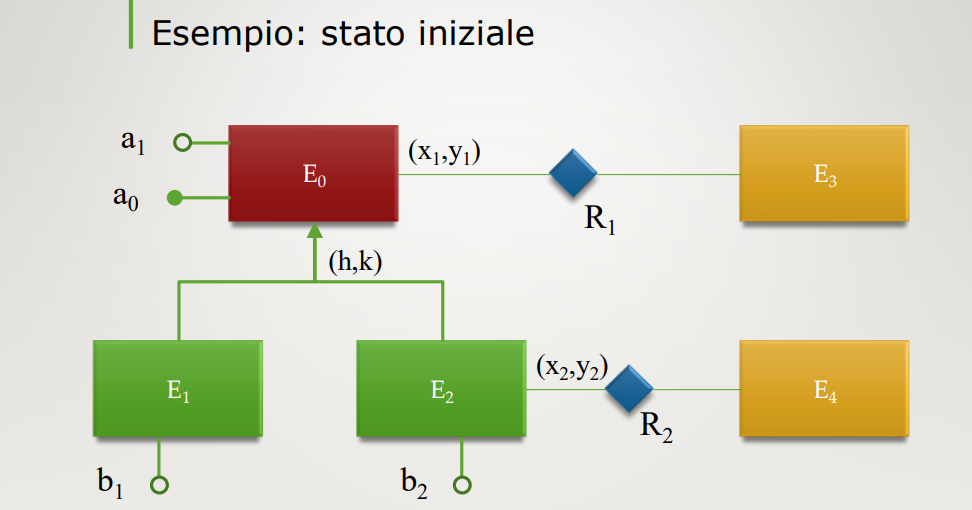
\includegraphics[width=1\linewidth]{image34.png}
    \caption{Stato iniziale}
\end{figure}
\begin{figure}[H]
    \centering
    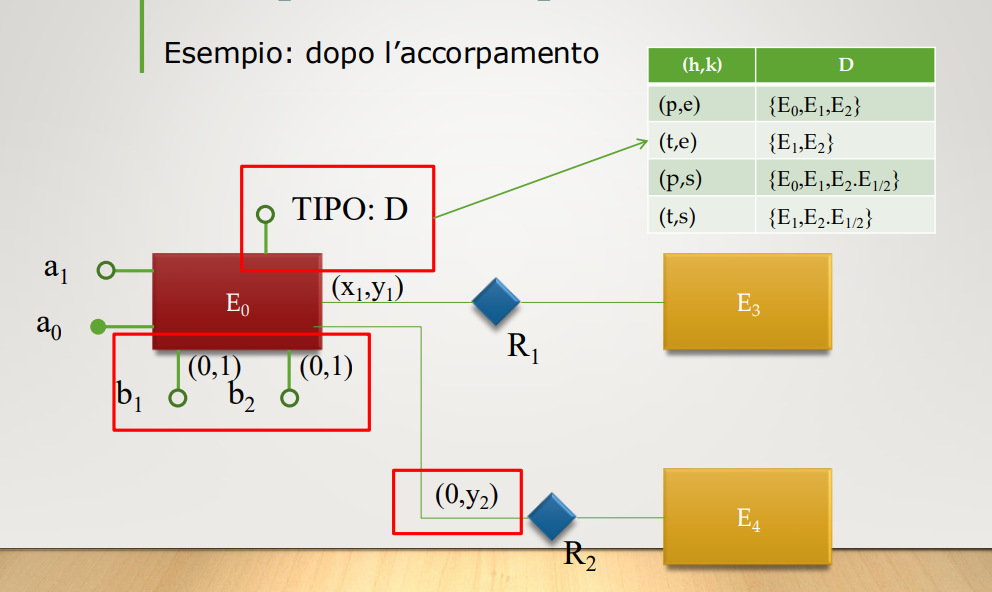
\includegraphics[width=1\linewidth]{image35.png}
    \caption{Accorpamento delle entità figlie nel padre}
\end{figure}
\subsubsection{Accorpamento del padre nelle entità figlie}

Questa trasformazione può essere applicata solo quando la generalizzazione è \textbf{totale}.  
La procedura consiste nei seguenti passi:
\begin{itemize}
    \item Eliminazione dell’entità padre.
    \item Replicazione degli attributi dell’entità padre in ciascuna entità figlia.
    \item Partizionamento, tra le entità figlie, delle relazioni che coinvolgevano l’entità padre, assegnando \textbf{cardinalità minima pari a 0} dal lato delle entità esterne.
\end{itemize}

\begin{figure}[H]
    \centering
    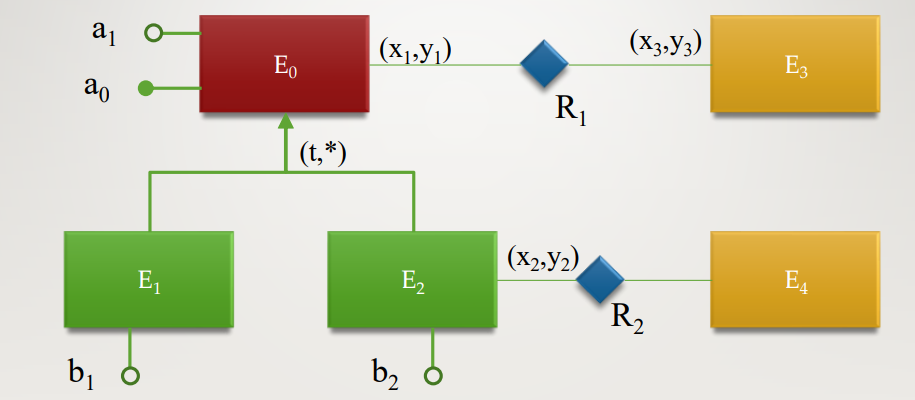
\includegraphics[width=1\linewidth]{image36.png}
    \caption{Schema iniziale}
\end{figure}

\begin{figure}[H]
    \centering
    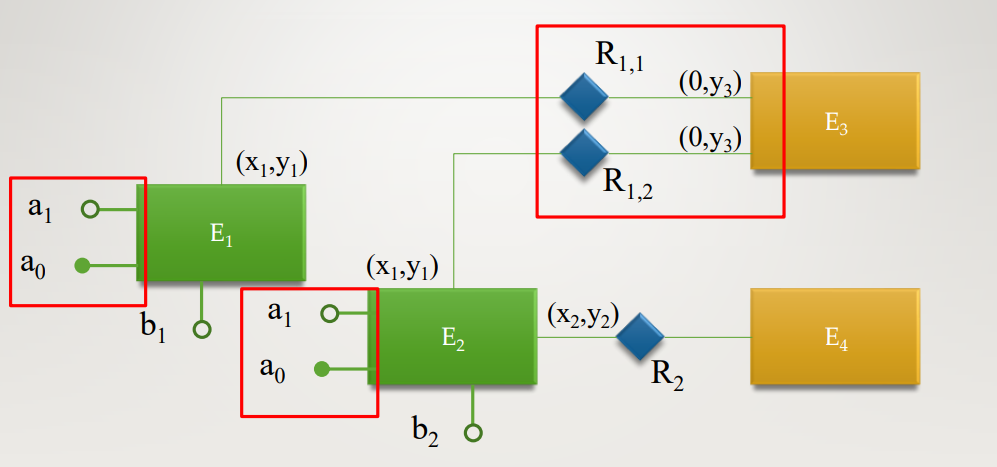
\includegraphics[width=1\linewidth]{image37.png}
    \caption{Accorpamento nelle entità figlie}
\end{figure}
\subsubsection{Sostituzione con relazioni}

Questa strategia sostituisce la generalizzazione con un insieme di relazioni esplicite.  
I passi da seguire sono:
\begin{itemize}
    \item Eliminazione della generalizzazione.
    \item Inserimento di $n$ relazioni tra l’entità padre e ciascuna delle $n$ entità figlie.
    \item Mantenimento degli attributi nelle entità in cui si trovavano originalmente, senza spostamenti.
\end{itemize}

\begin{figure}[H]
    \centering
    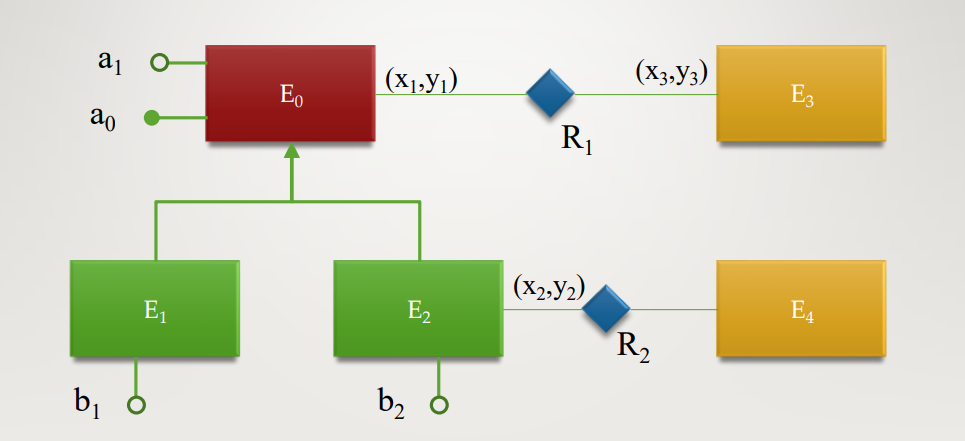
\includegraphics[width=1\linewidth]{image38.png}
    \caption{Schema iniziale}
\end{figure}

\begin{figure}[H]
    \centering
    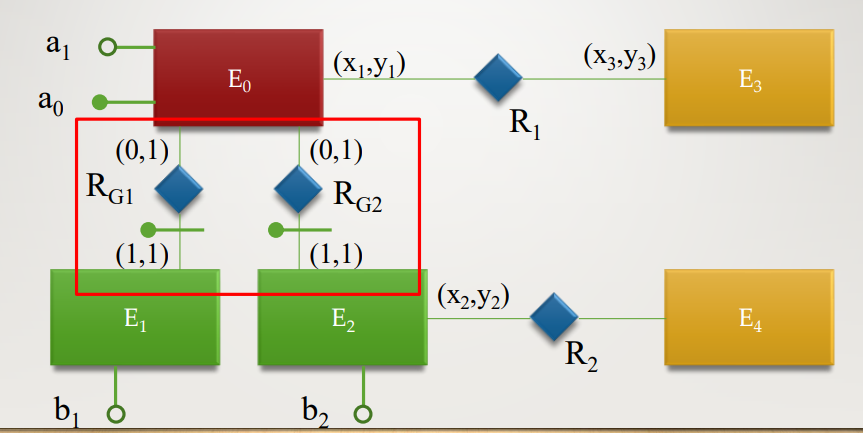
\includegraphics[width=1\linewidth]{image39.png}
    \caption{Sostituzione della generalizzazione con relazioni}
\end{figure}
\subsection{Traduzione verso il modello relazionale}

La traduzione verso il modello relazionale è un processo automatico che applica allo \textbf{schema concettuale ristrutturato} un insieme di regole di trasformazione.  
Ogni regola si applica a uno specifico costrutto del modello concettuale ER e produce una o più strutture del modello relazionale.

I principi fondamentali della traduzione sono:
\begin{itemize}
    \item Un’\textbf{istanza di entità} viene rappresentata mediante una \textbf{tupla} della tabella che implementa l’entità.
    \item Un’\textbf{istanza di relazione} viene rappresentata tramite:
    \begin{itemize}
        \item un \textbf{legame tra tuple} (mediante chiavi esterne), oppure
        \item una \textbf{tupla esplicita} in una tabella dedicata.
    \end{itemize}
    \item L’\textbf{identificatore principale} di un’entità viene rappresentato come \textbf{chiave primaria} della tabella che implementa tale entità.
\end{itemize}
\subsection{Classificazione delle relazioni binarie}

Una relazione binaria del modello ER può assumere tre forme, in base alle \textbf{cardinalità massime} delle entità coinvolte:

\begin{itemize}
    \item \textbf{Uno a Uno (1:1)}:  
    entrambe le entità coinvolte nella relazione hanno cardinalità massima pari a 1.

    \item \textbf{Uno a Molti (1:N)}:  
    una delle entità ha cardinalità massima pari a 1, mentre l’altra ha cardinalità massima maggiore di 1.

    \item \textbf{Molti a Molti (N:M)}:  
    entrambe le entità hanno cardinalità massima maggiore di 1.
\end{itemize}
\subsection{Regole di traduzione}
\begin{figure}[H]
    \centering
    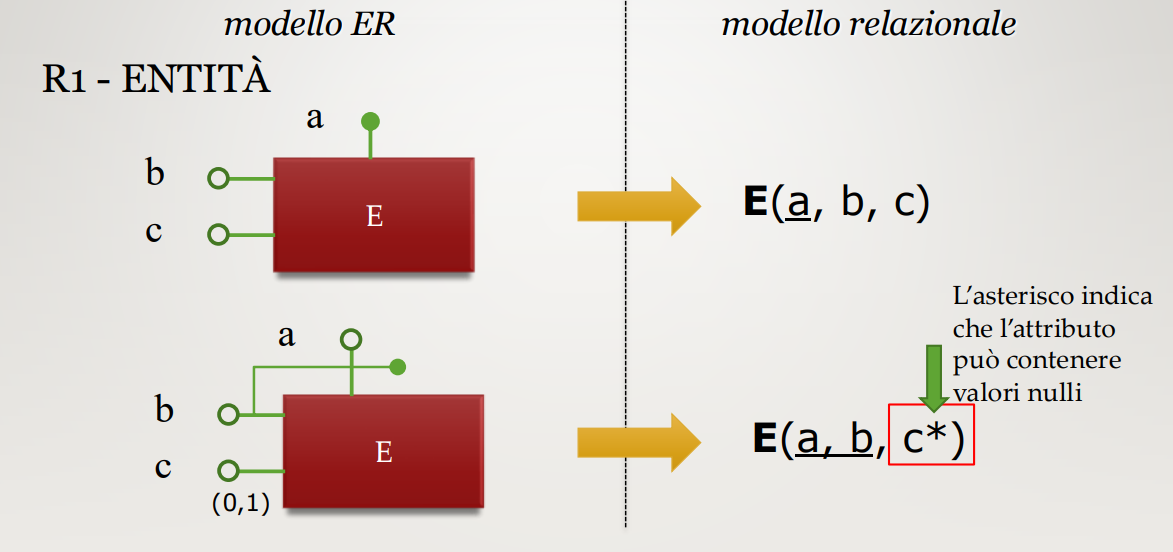
\includegraphics[width=1\linewidth]{image40.png}
    \caption{Entità}
\end{figure}
\begin{figure}[H]
    \centering
    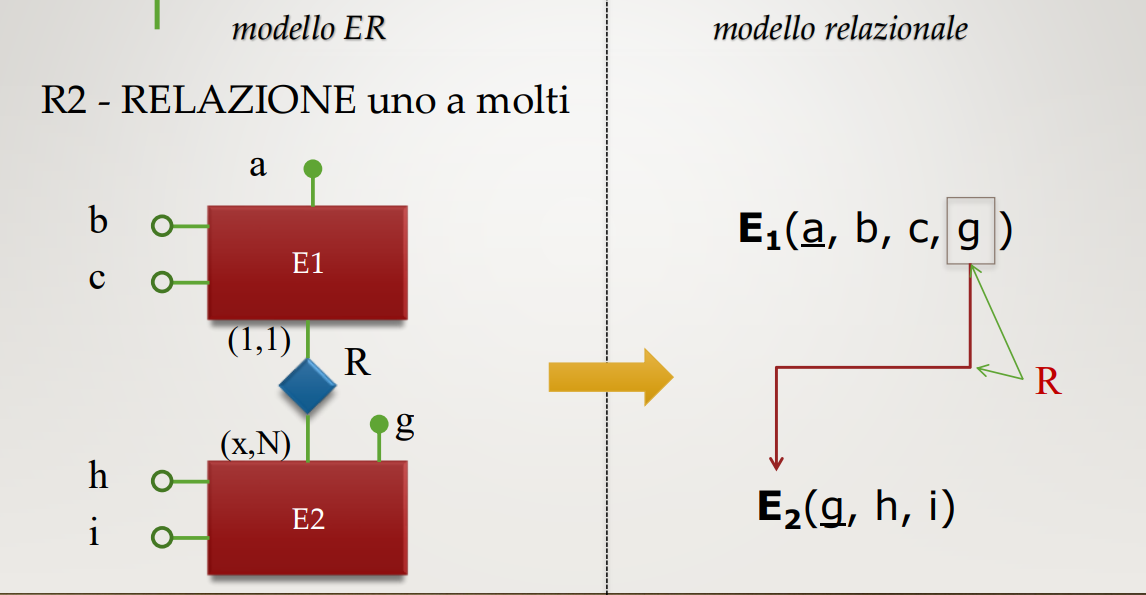
\includegraphics[width=1\linewidth]{image41.png}
    \caption{Relazione uno a molti}
\end{figure}
\begin{figure}[H]
    \centering
    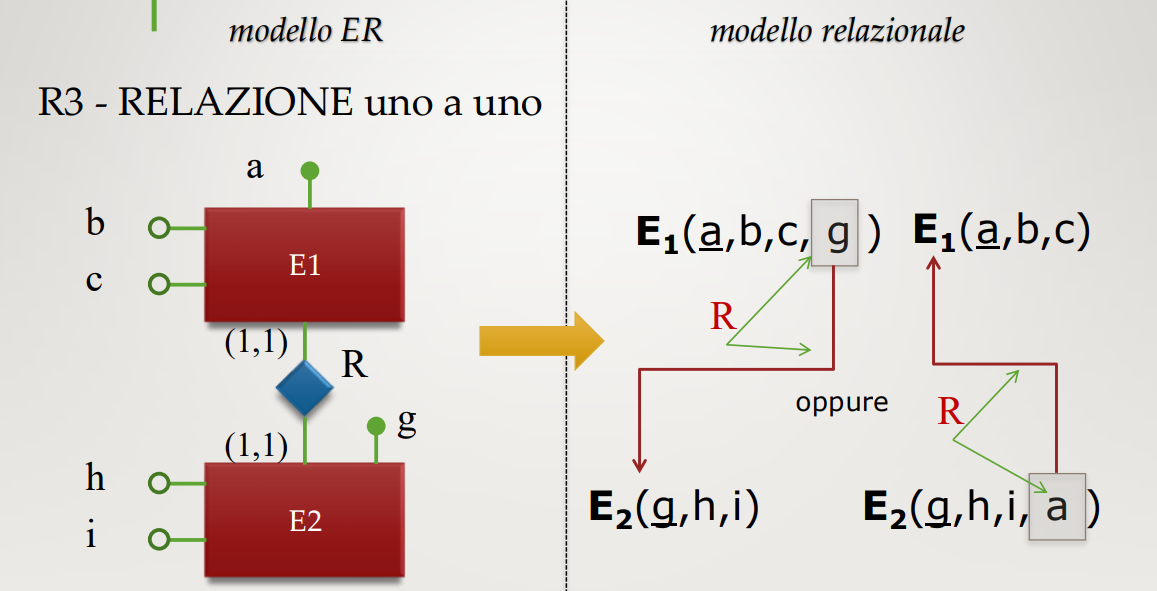
\includegraphics[width=1\linewidth]{image42.png}
    \caption{Relazione uno a uno}
\end{figure}
\begin{figure}[H]
    \centering
    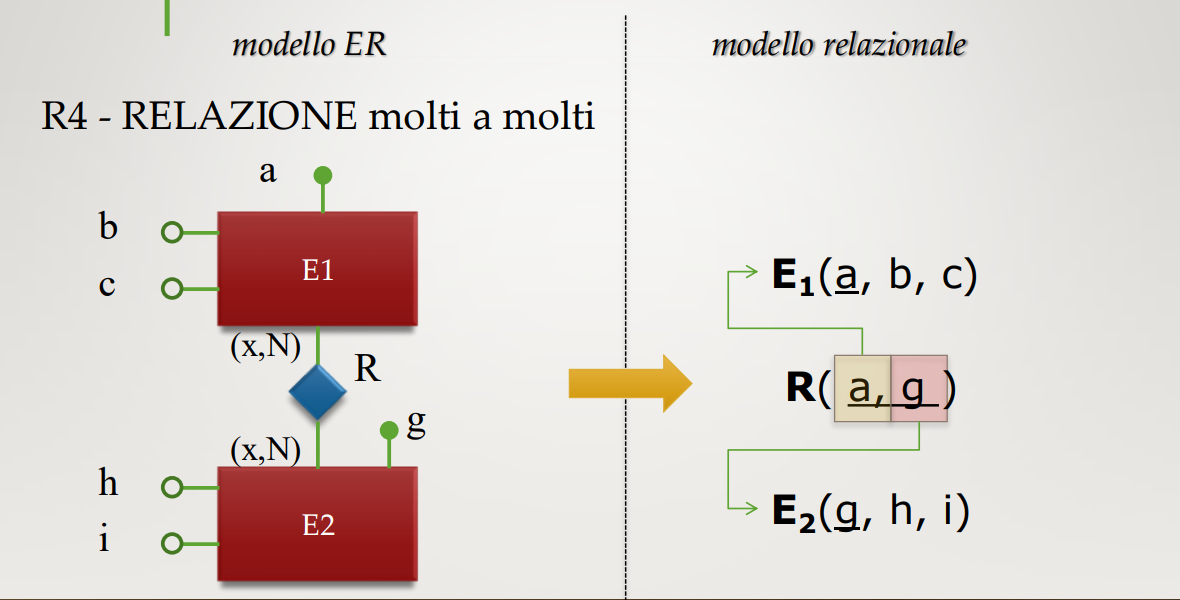
\includegraphics[width=1\linewidth]{image43.png}
    \caption{Relazione molti a molti}
\end{figure}
\begin{figure}[H]
    \centering
    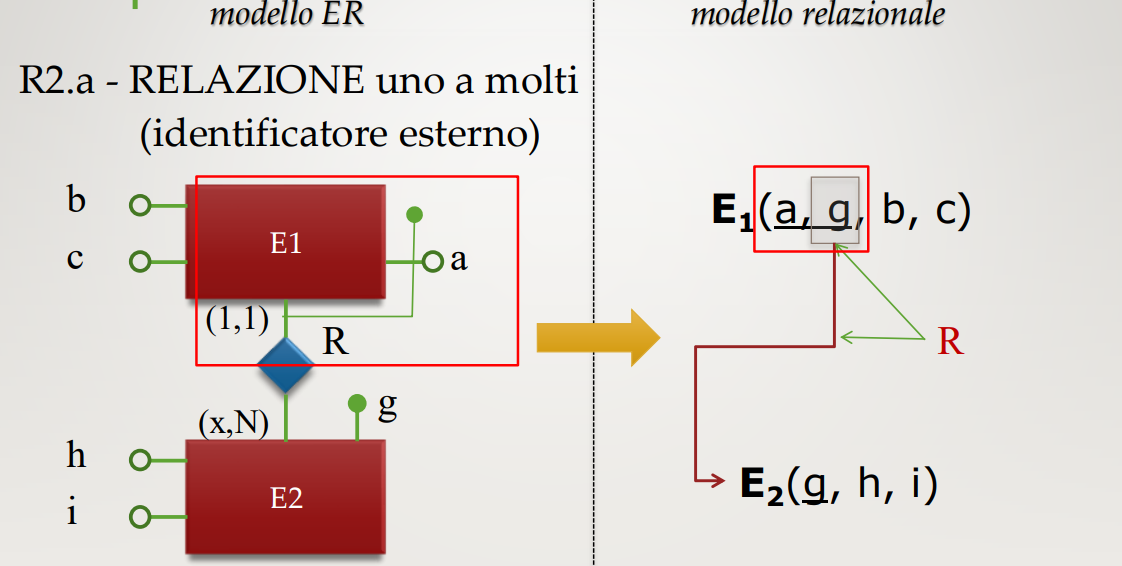
\includegraphics[width=1\linewidth]{image44.png}
    \caption{Relazione uno a molti identificatore esterno}
\end{figure}
\begin{figure}[H]
    \centering
    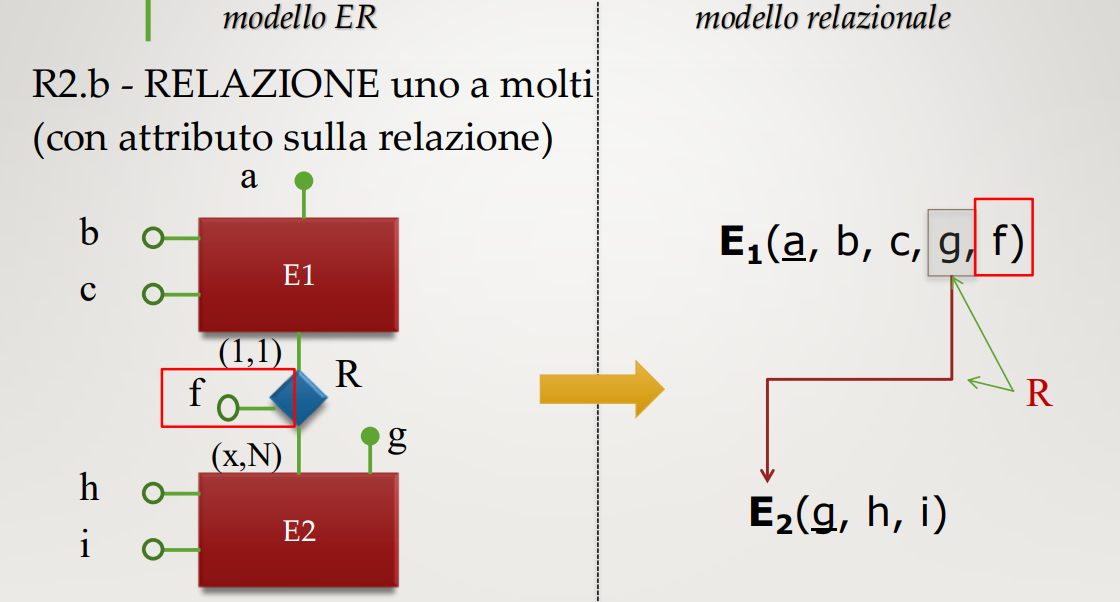
\includegraphics[width=1\linewidth]{image45.png}
    \caption{Relazione uno a molti con attributo sulla relazione}
\end{figure}
\begin{figure}[H]
    \centering
    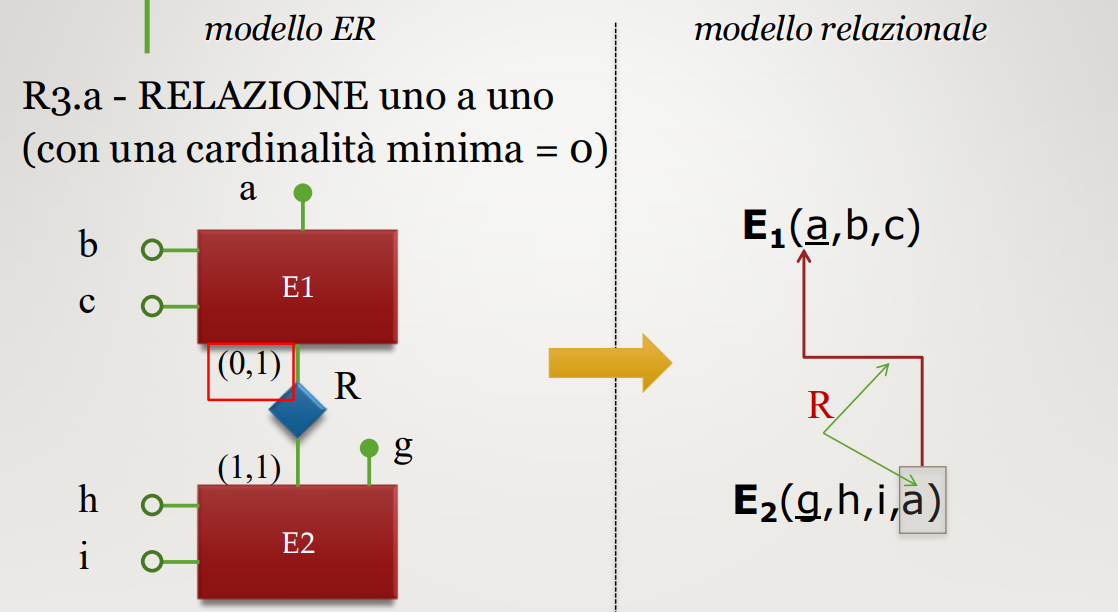
\includegraphics[width=1\linewidth]{image46.png}
    \caption{RELAZIONE uno a uno
(con una cardinalità minima = 0)}
\end{figure}
\begin{figure}[H]
    \centering
    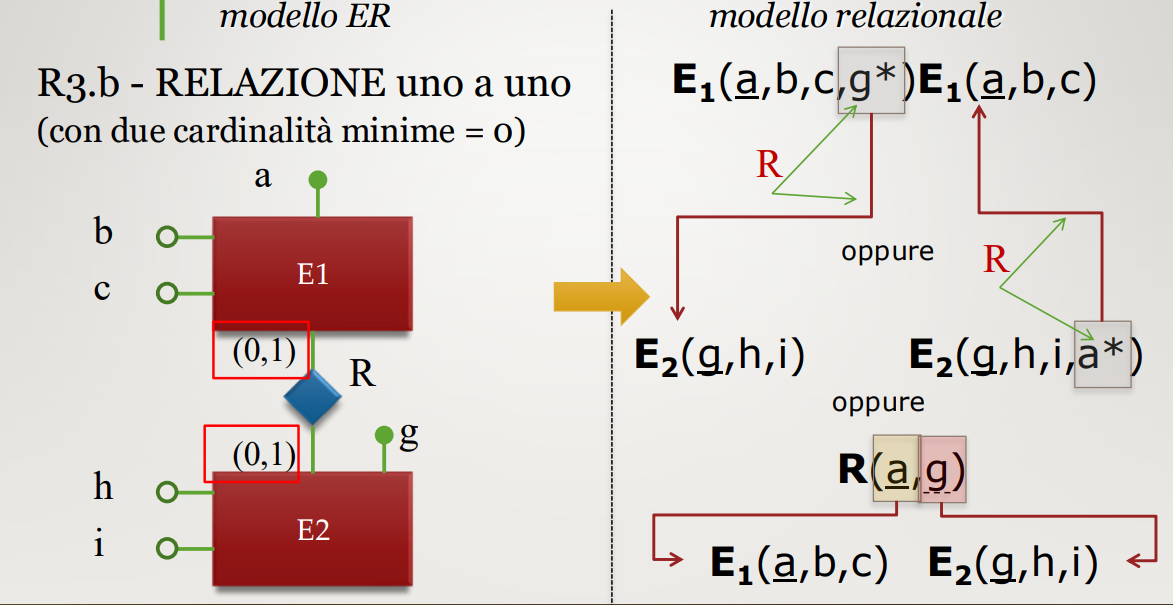
\includegraphics[width=1\linewidth]{image47.png}
    \caption{RELAZIONE uno a uno
(con due cardinalità minime = 0)}
\end{figure}
\begin{figure}[H]
    \centering
    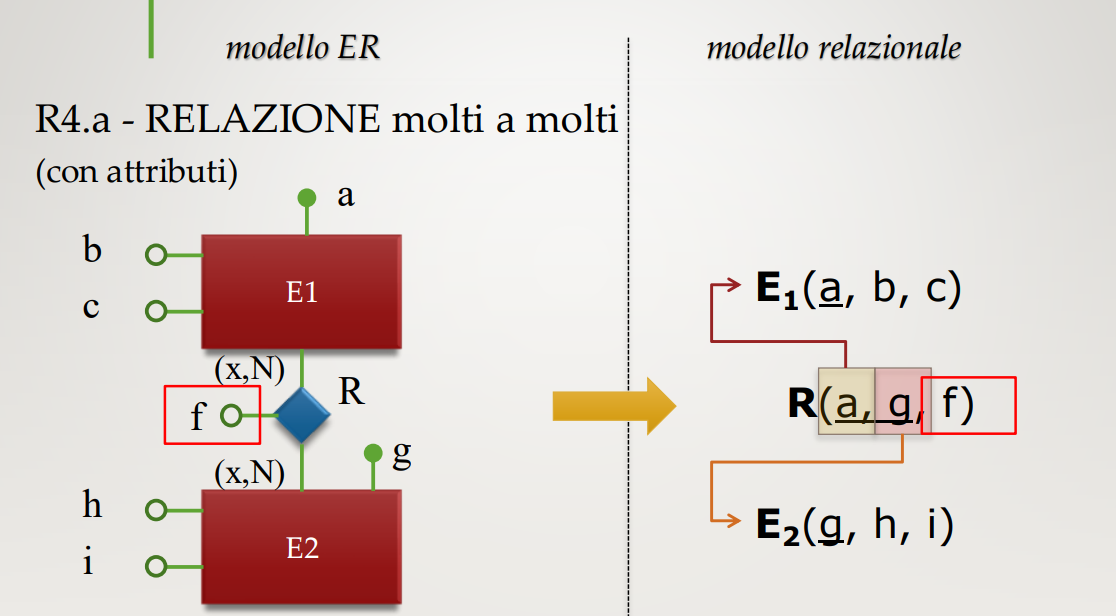
\includegraphics[width=1\linewidth]{image48.png}
    \caption{ - RELAZIONE molti a molti
(con attributi)}
\end{figure}
\begin{figure}[H]
    \centering
    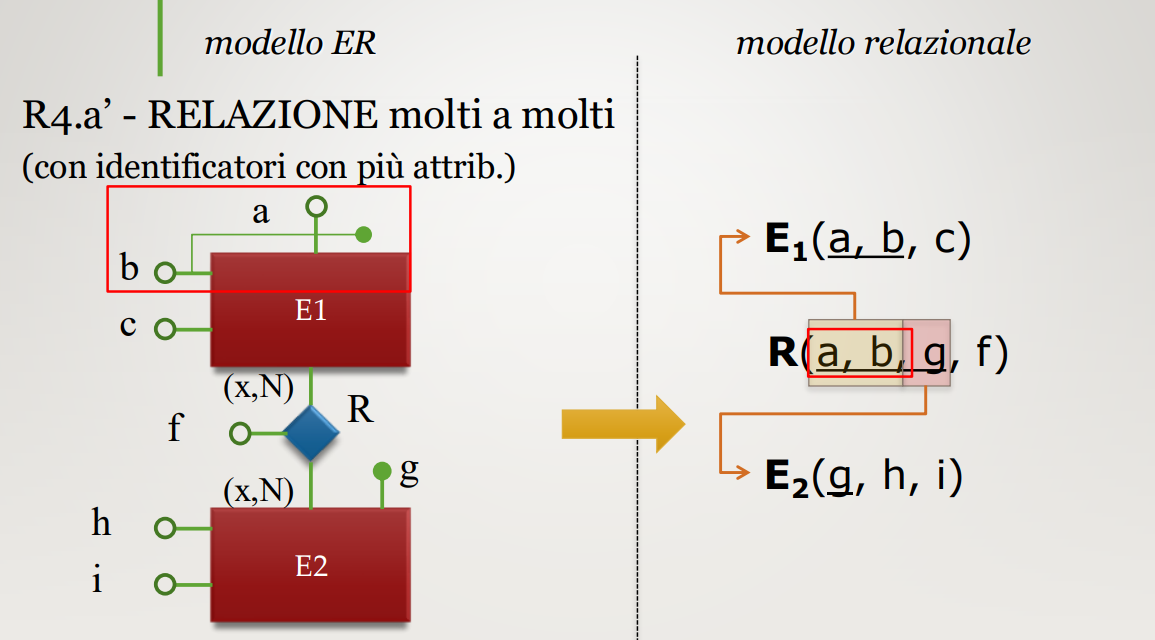
\includegraphics[width=1\linewidth]{image49.png}
    \caption{RELAZIONE molti a molti
(con identificatori con più attrib.) }
\end{figure}
\begin{figure}[H]
    \centering
    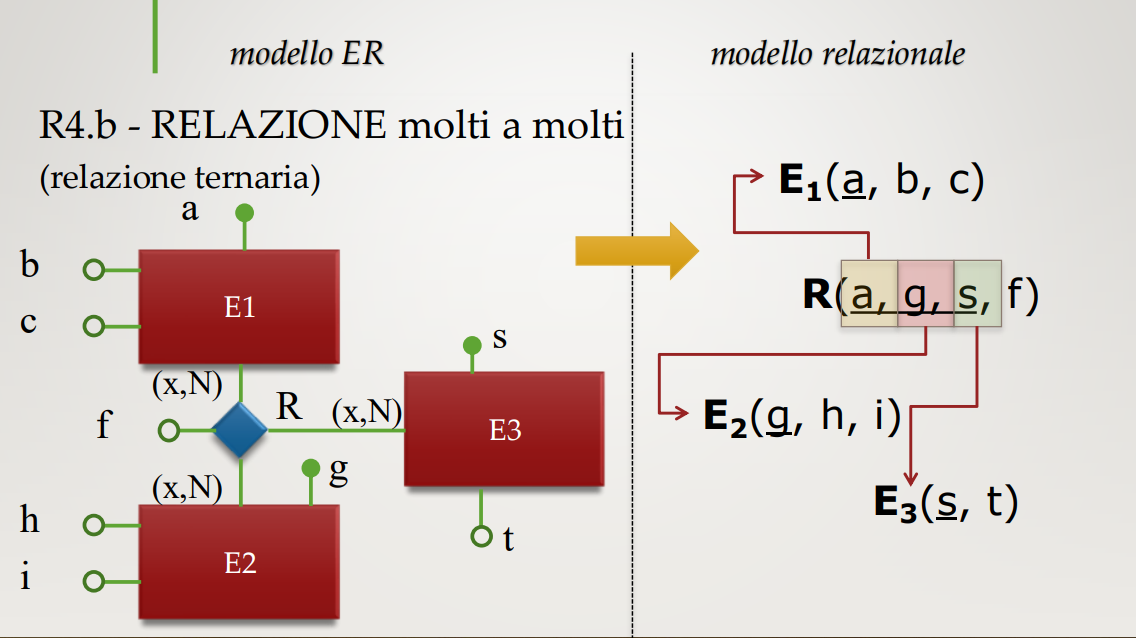
\includegraphics[width=1\linewidth]{image50.png}
    \caption{RELAZIONE molti a molti
(relazione ternaria)
}
\end{figure}
\begin{figure}[H]
    \centering
    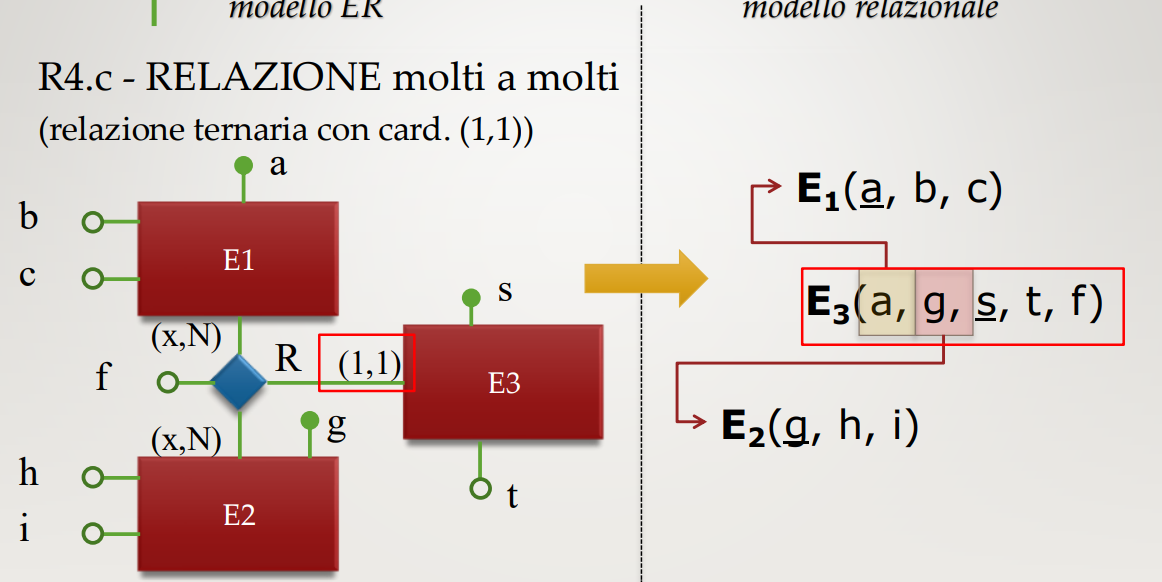
\includegraphics[width=1\linewidth]{image51.png}
    \caption{RELAZIONE molti a molti
(relazione ternaria con card. (1,1))}
    \label{fig:placeholder}
\end{figure}
	\section{Tecnologie NoSQL: Sistemi Document-Based}

\begin{figure}[H]
    \centering
    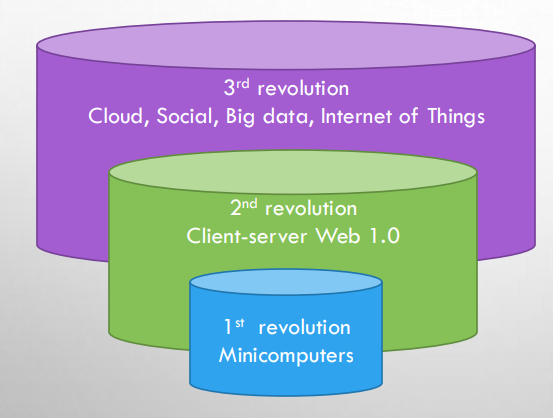
\includegraphics[width=0.75\linewidth]{image52.png}
    \caption{Evoluzione Database}
\end{figure}

La figura mostra l'evoluzione storica delle tecnologie di database attraverso
tre grandi rivoluzioni, rappresentate come livelli sovrapposti. Ogni rivoluzione
introduce nuovi modelli, nuovi paradigmi e nuove esigenze dovute ai cambiamenti
tecnologici del periodo.

\subsection*{Prima rivoluzione (1950--1960)}
Alla base si trova la prima rivoluzione dei database, nata nell'epoca dei
\textbf{minicomputer}. In questo periodo emergono i primi sistemi per la gestione
dei dati, caratterizzati da strutture rigide e fortemente dipendenti
dall'organizzazione fisica dei file. Le principali tecnologie di questo periodo sono:
\begin{itemize}
    \item database \textbf{gerarchici};
    \item database \textbf{reticolari} (network databases);
    \item file organizzati tramite \textbf{ISAM} (Indexed Sequential Access Method).
\end{itemize}

\subsection*{Seconda rivoluzione (1970--1990)}
Il secondo livello corrisponde alla diffusione del modello \textbf{relazionale},
che nasce negli anni '70 grazie ai lavori di E. F. Codd. In questa fase il
paradigma relazionale si impone come standard grazie alla sua semplicità,
astrazione e indipendenza dalla struttura fisica dei dati.
È l'epoca dei sistemi \textbf{client-server} e del Web~1.0.

\subsection*{Terza rivoluzione (2005--oggi)}
La terza rivoluzione si sviluppa nell'era del \textbf{cloud}, dei \textbf{big data}
e dell'\textbf{Internet of Things}. In questo contesto il volume, la varietà e la
velocità dei dati aumentano notevolmente, rendendo necessarie nuove soluzioni
oltre al modello relazionale classico. Accanto ai database tradizionali si
diffondono:
\begin{itemize}
    \item sistemi \textbf{NoSQL};
    \item sistemi \textbf{NewSQL};
    \item piattaforme di \textbf{Big Data}.
\end{itemize}

Questa rivoluzione rappresenta un ampliamento, non una sostituzione: i database
relazionali restano fondamentali, ma vengono affiancati da tecnologie progettate
per gestire grandi moli di dati distribuiti.

\subsection{Approcci NoSQL}
I modelli NoSQL nascono per rispondere ai limiti dei tradizionali database
relazionali in scenari caratterizzati da grandi quantità di dati, alta
eterogeneità e necessità di scalare orizzontalmente. Questi sistemi adottano
strutture più flessibili e meno vincolate rispetto allo schema rigido delle
tabelle relazionali, permettendo una gestione più efficiente di dati distribuiti
su larga scala. Tra gli approcci più diffusi troviamo:
\begin{itemize}
    \item \textbf{Sistemi Key-Value}: tutti i dati sono rappresentati tramite coppie
    (chiave, valore), dove la chiave identifica le istanze e il valore può avere
    una qualsiasi struttura, anche non omogenea. Un esempio di questo approccio
    è Hadoop.

    \item \textbf{Sistemi Document-Store}: i dati sono rappresentati come collezioni
    di documenti con struttura complessa e senza schema fisso.
    Esempi: \textbf{MongoDB}, \textbf{CouchBase}.

    \item \textbf{Column Store}: i dati sono rappresentati tramite record con struttura variabile.
    Esempi: \textbf{BigTable}, \textbf{HBase}, \textbf{Cassandra}.

    \item \textbf{Graph-Store}: i dati sono rappresentati come grafi, con nodi e archi.
    Esempi: \textbf{Neo4j}, \textbf{OrientDB}.
\end{itemize}

\subsection{Sistemi Document-Store}
Caratteristiche principali:
\begin{itemize}
    \item i dati sono organizzati come collezioni di \textbf{documenti};
    \item ogni documento può contenere dati complessi e nidificati;
    \item l'\textbf{incapsulamento} è fondamentale: tutte le informazioni relative a un'entità
    stanno nello stesso documento;
    \item non è richiesto uno schema fisso: i documenti di una collezione possono avere
    strutture diverse.
\end{itemize}

\subsubsection*{Progettazione dei dati come documenti}
Decisioni fondamentali:
\begin{itemize}
    \item scelta della chiave di accesso;
    \item struttura interna dei documenti e livello di incapsulamento;
    \item rappresentazione delle relazioni tra documenti.
\end{itemize}

Le relazioni possono essere modellate tramite:
\begin{itemize}
    \item \textbf{riferimenti} (ID dell’altro documento);
    \item \textbf{documenti nidificati}.
\end{itemize}

\begin{figure}[H]
    \centering
    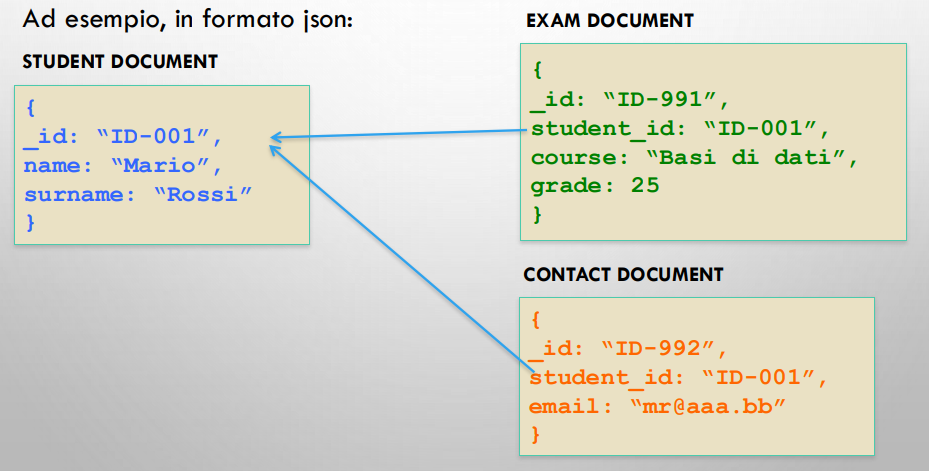
\includegraphics[width=0.75\linewidth]{image53.png}
    \caption{Formato JSON}
\end{figure}

\subsection{Regole di traduzione di uno schema ER in collezioni di documenti}

Assunzioni preliminari:
\begin{itemize}
    \item si adotta un approccio \textbf{embedded};
    \item lo schema ER è privo di generalizzazioni;
    \item relazioni ternarie o superiori eliminate;
    \item identificate collezioni \(\{DOC_1, ..., DOC_N\}\).
\end{itemize}

\subsubsection*{Regole fondamentali}
\begin{enumerate}
    \item Ogni collezione \(DOC_i\) corrisponde a un'entità principale.
    \item Ogni istanza dell'entità principale produce un documento.
    \item Le entità non principali vengono incapsulate nella principale.
    \item Le relazioni sono rappresentate tramite incapsulamento o riferimenti.
\end{enumerate}

\subsubsection{Prima Fase (entità principali)}
\begin{figure}[H]
    \centering
    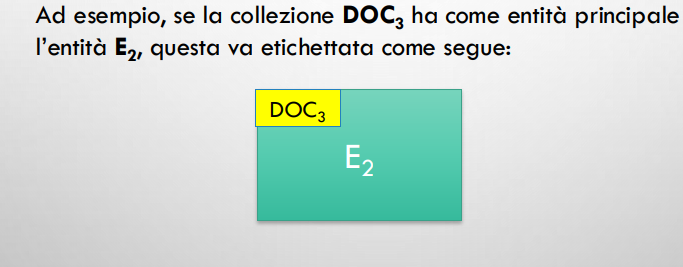
\includegraphics[width=1\linewidth]{image56.png}
    \caption{Individuazione entità principali}
\end{figure}

\subsubsection{Seconda Fase (incapsulamento entità non principali)}
\begin{figure}[H]
    \centering
    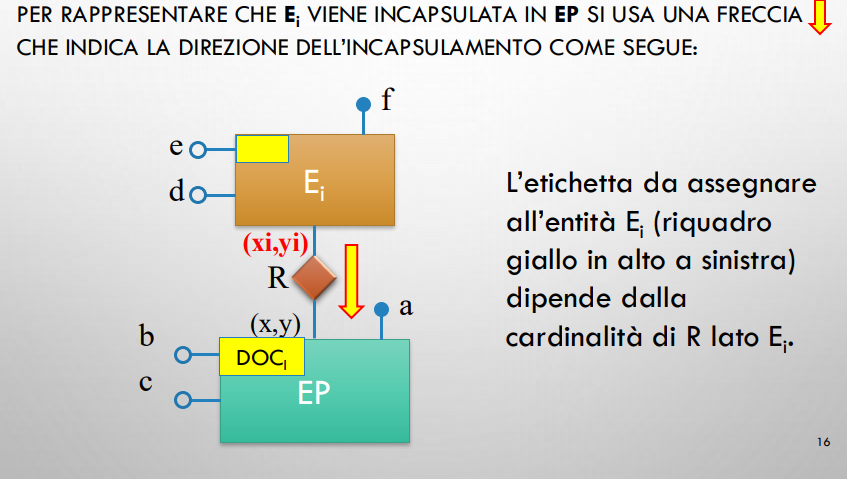
\includegraphics[width=0.75\linewidth]{image57.png}
    \caption{Incapsulamento}
\end{figure}

\subsection*{Diversi Casi}
\begin{figure}[H]
    \centering
    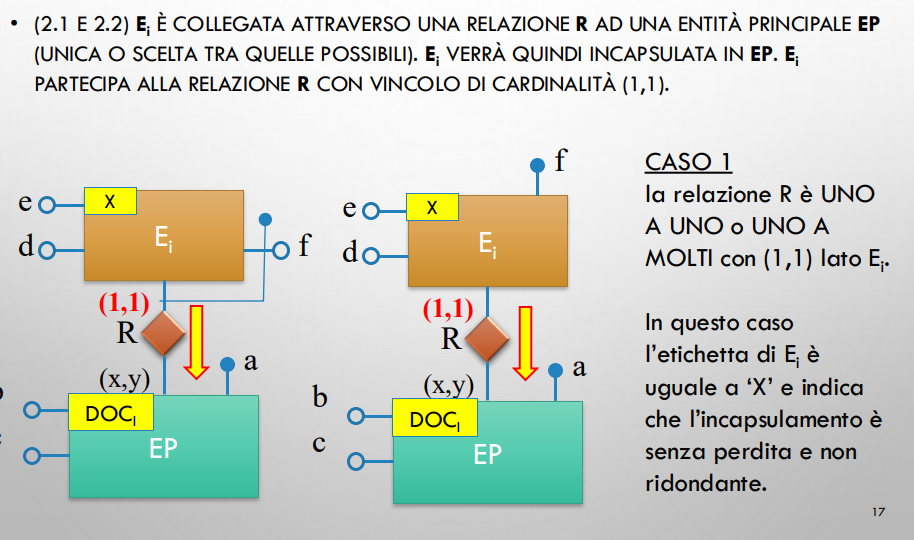
\includegraphics[width=1\linewidth]{image58.png}
    \caption{Uno a uno o uno a molti con (1,1)}
\end{figure}

\begin{figure}[H]
    \centering
    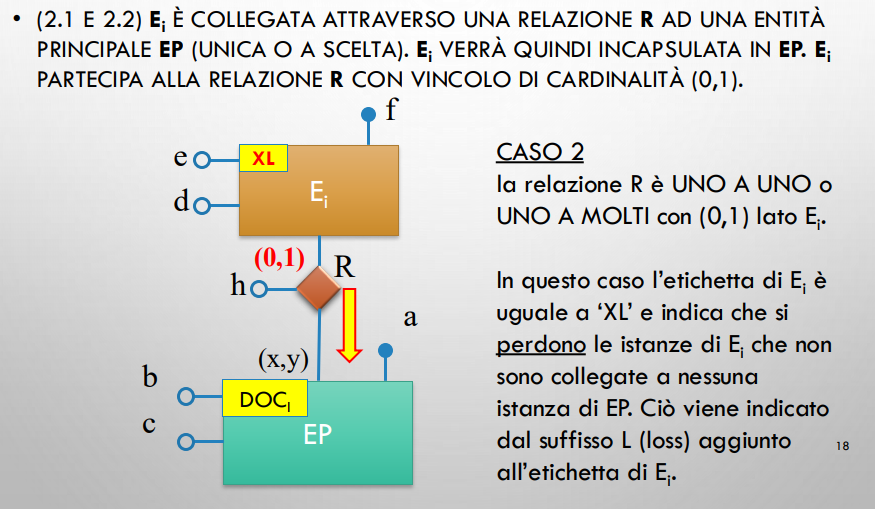
\includegraphics[width=1\linewidth]{image59.png}
    \caption{Uno a uno o uno a molti con (0,1)}
\end{figure}

\begin{figure}[H]
    \centering
    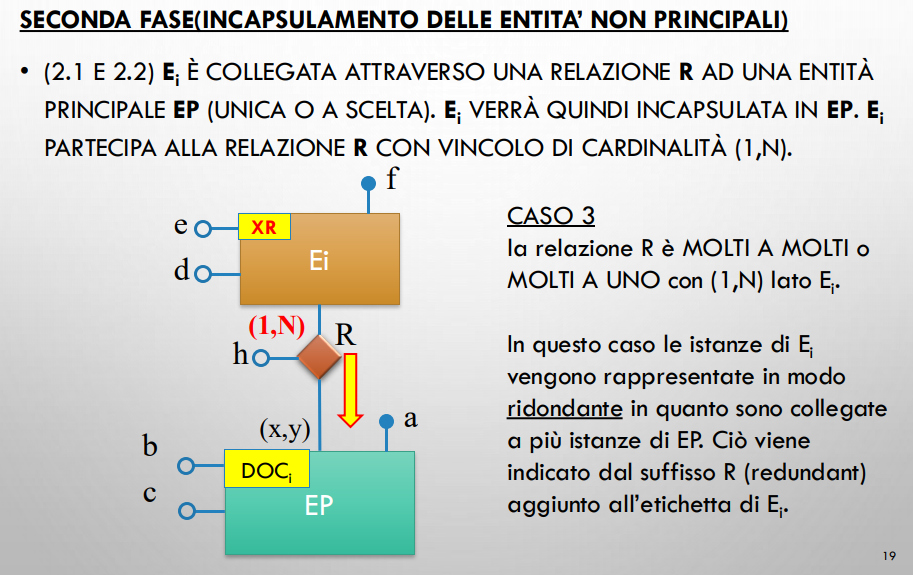
\includegraphics[width=1\linewidth]{image60.png}
    \caption{Molti a molti o molti a uno con (1,N)}
\end{figure}

\begin{figure}[H]
    \centering
    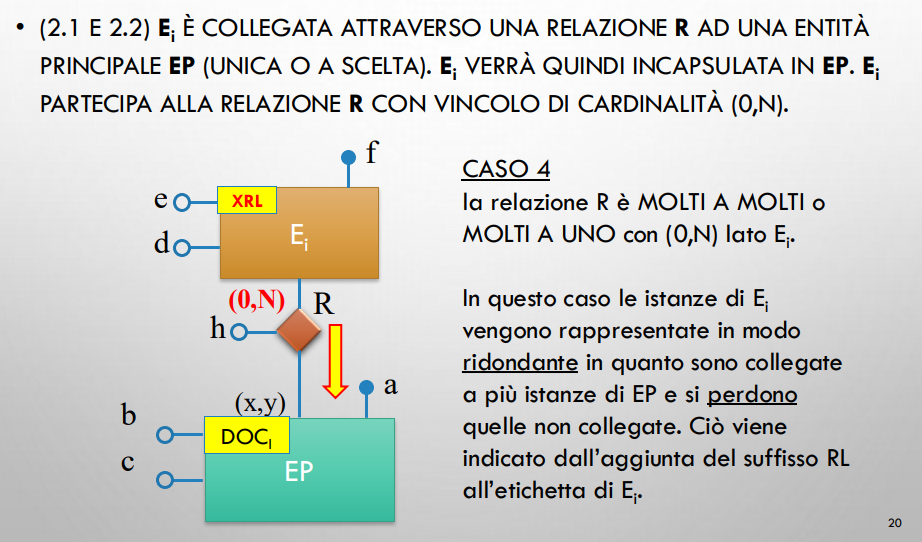
\includegraphics[width=1\linewidth]{image61.png}
    \caption{Molti a molti o molti a uno con (0,N) lato Ei}
\end{figure}

\subsubsection{Terza Fase (relazioni non strutturali)}
\begin{figure}[H]
    \centering
    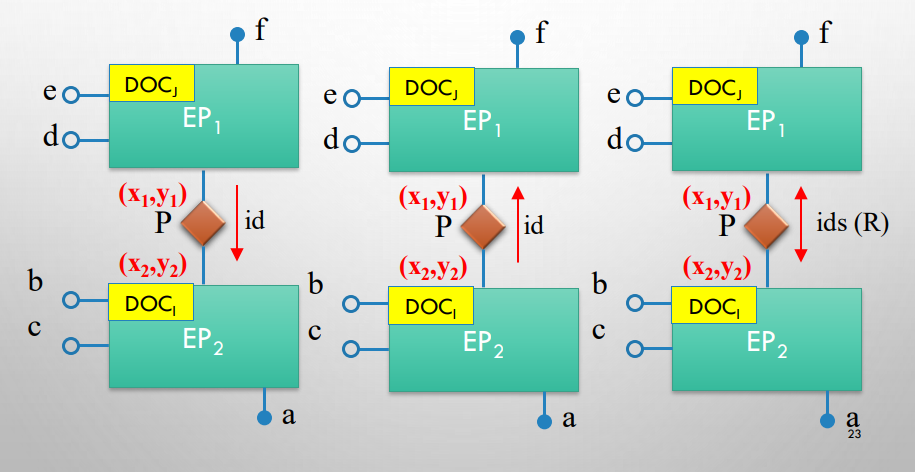
\includegraphics[width=1\linewidth]{image63.png}
    \caption{Etichettatura dello schema ER}
\end{figure}

\subsubsection*{Casi particolari}
\begin{figure}[H]
    \centering
    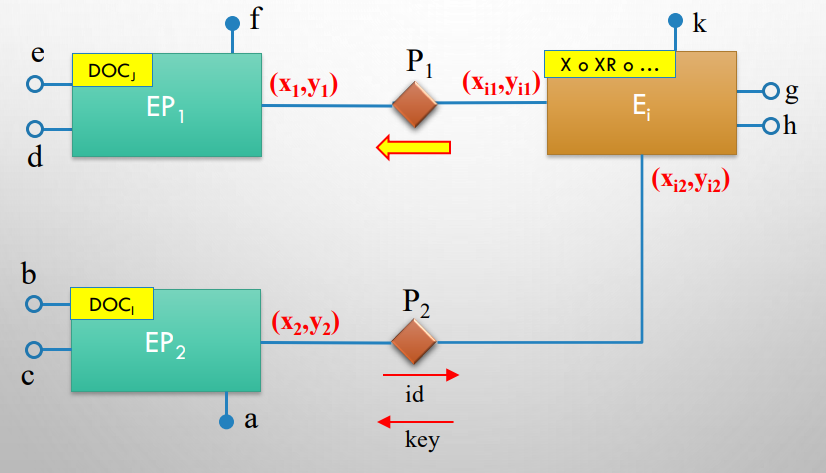
\includegraphics[width=1\linewidth]{image64.png}
    \caption{Caso Particolare A}
\end{figure}

\begin{figure}[H]
    \centering
    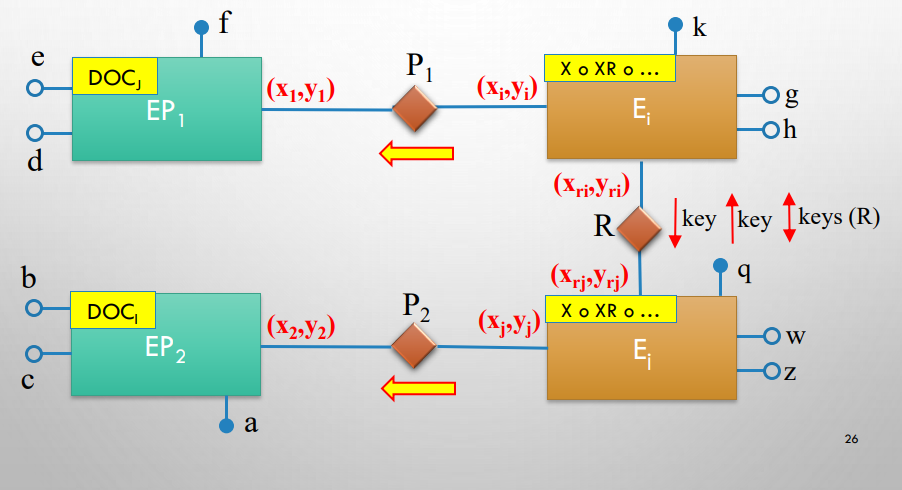
\includegraphics[width=1\linewidth]{image65.png}
    \caption{Caso Particolare B}
\end{figure}

\subsection{Quarta fase}
\begin{figure}[H]
    \centering
    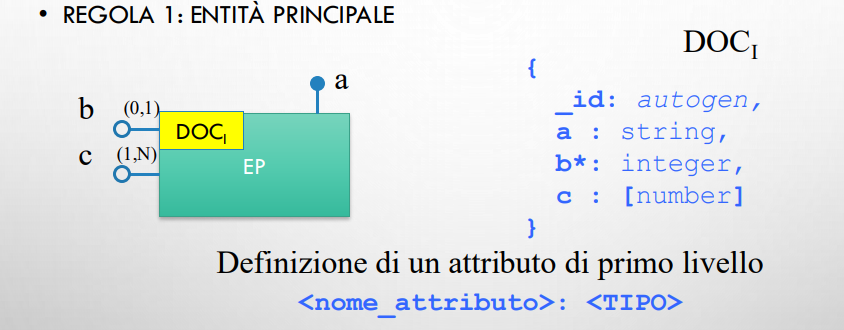
\includegraphics[width=1\linewidth]{image66.png}
    \caption{Entità Principale}
\end{figure}

\texttt{<TIPO>} può essere: string, integer, number, boolean, date, time, timestamp.

L'attributo \texttt{\_id} è sempre autogenerato dal sistema.

\begin{figure}[H]
\centering
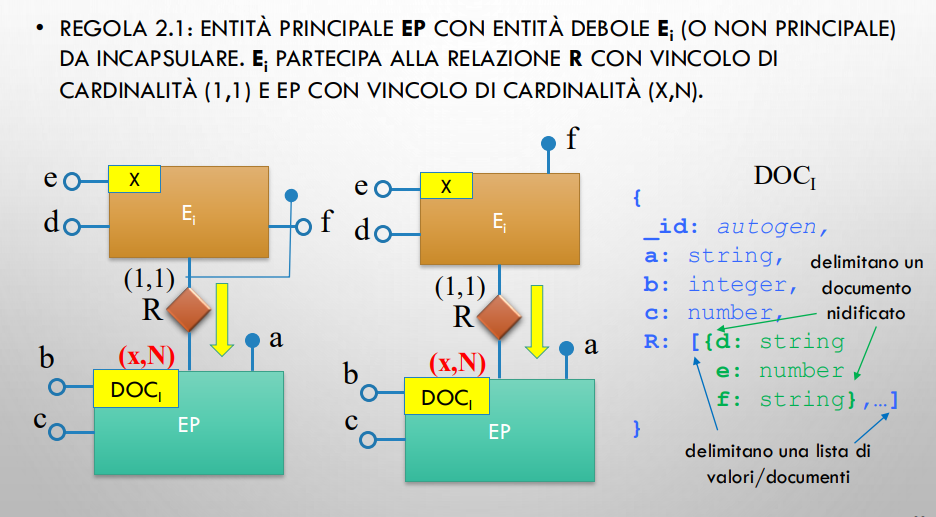
\includegraphics[width=1\linewidth]{image67.png}
\end{figure}

\begin{figure}[H]
\centering
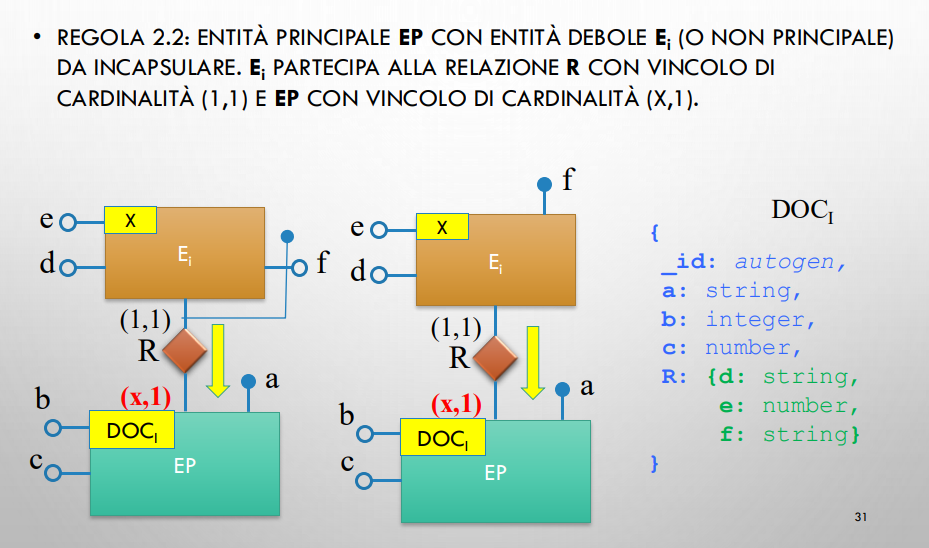
\includegraphics[width=1\linewidth]{image68.png}
\end{figure}

\begin{figure}[H]
\centering
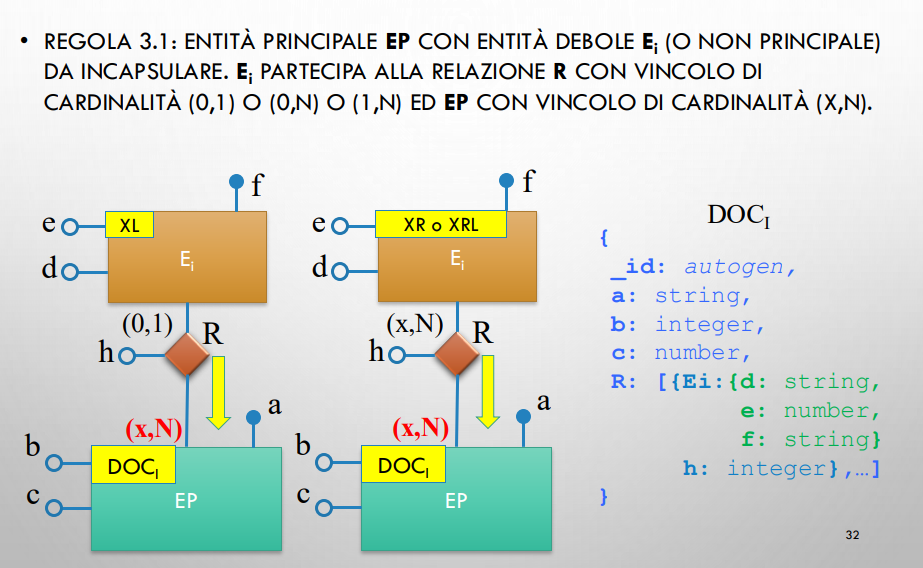
\includegraphics[width=1\linewidth]{image69.png}
\end{figure}

\begin{figure}[H]
\centering
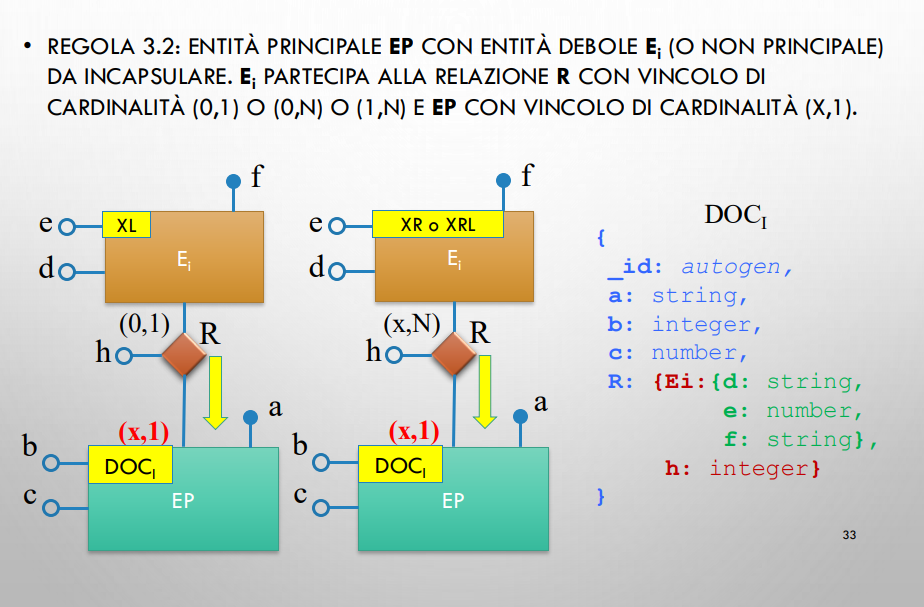
\includegraphics[width=1\linewidth]{image70.png}
\end{figure}

\begin{figure}[H]
\centering
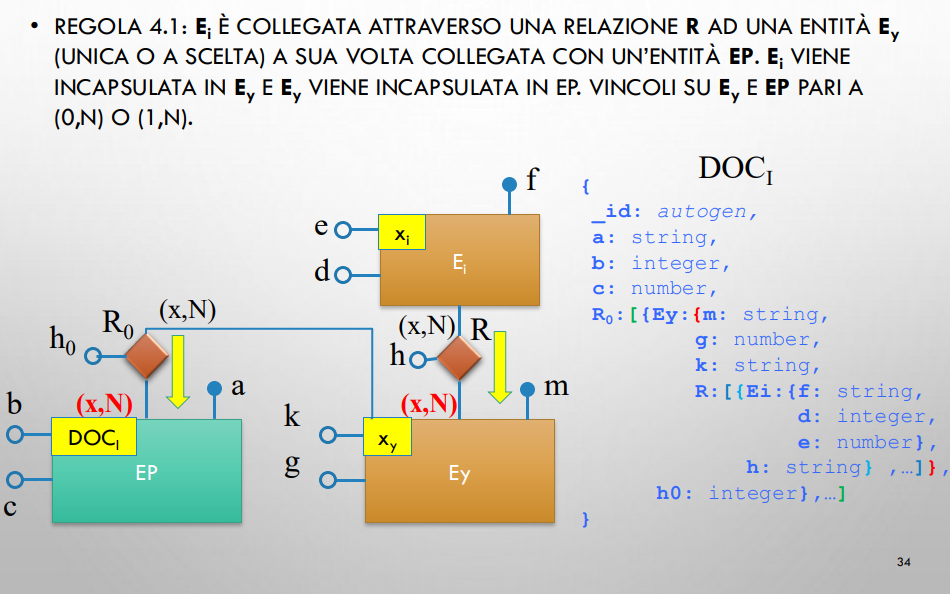
\includegraphics[width=1\linewidth]{image71.png}
\end{figure}

\begin{figure}[H]
\centering
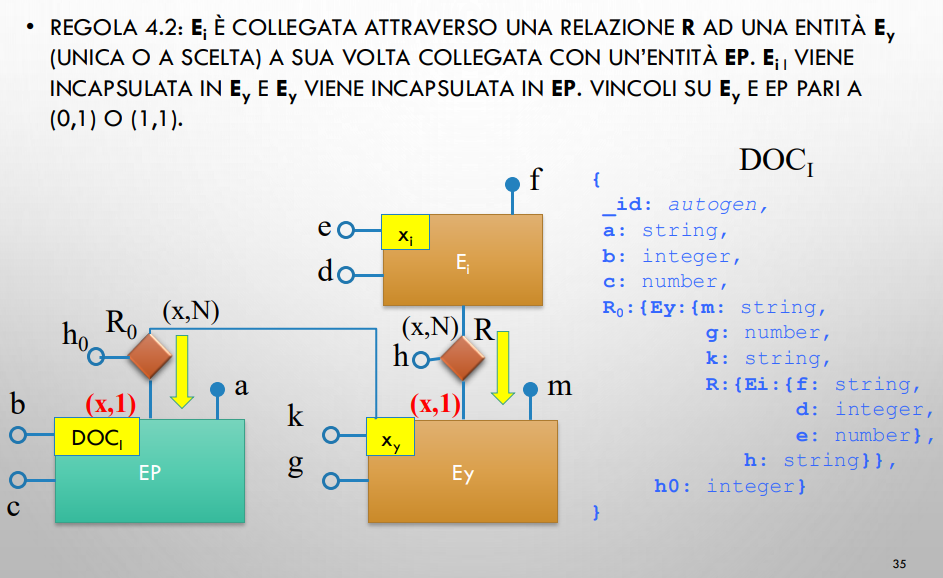
\includegraphics[width=1\linewidth]{image72.png}
\end{figure}

\begin{figure}[H]
\centering
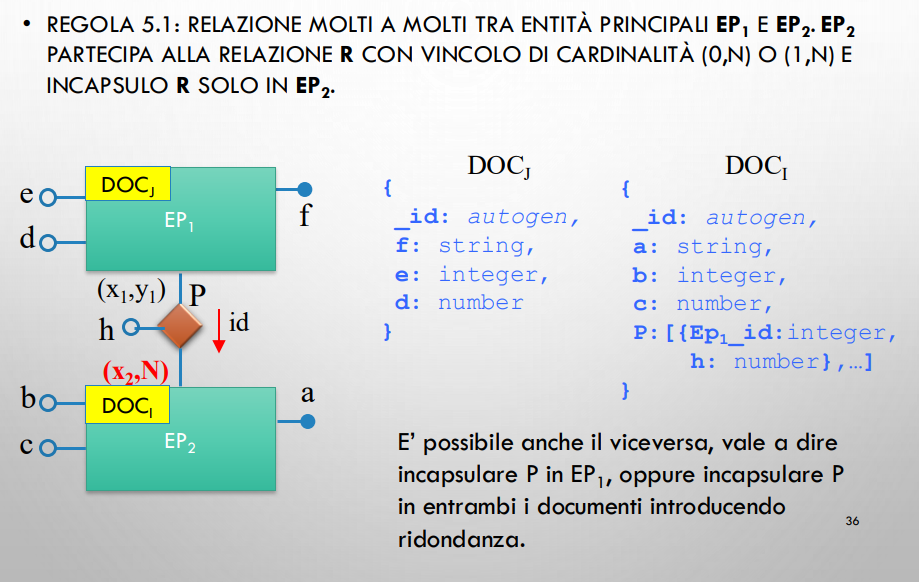
\includegraphics[width=1\linewidth]{image73.png}
\end{figure}

\begin{figure}[H]
\centering
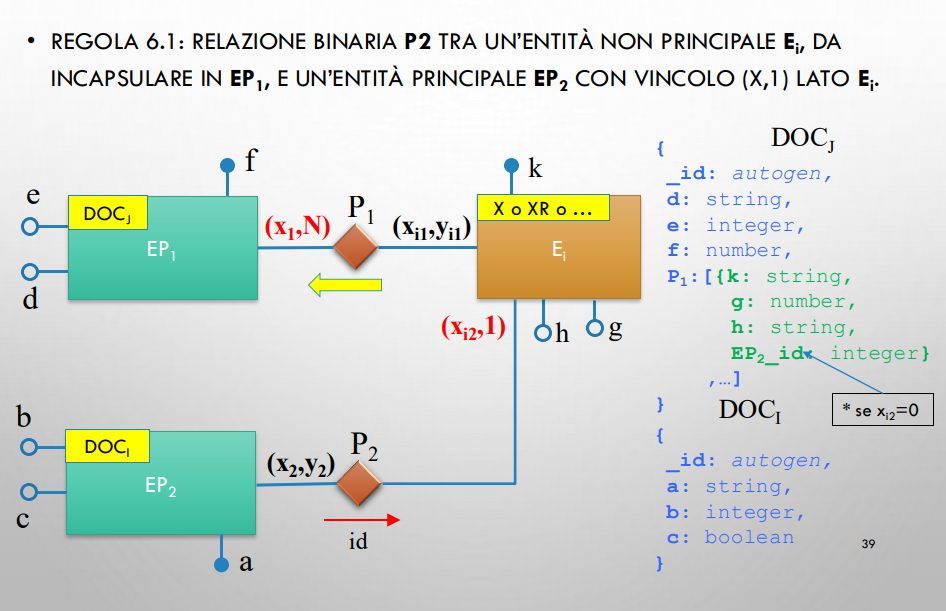
\includegraphics[width=1\linewidth]{image74.png}
\end{figure}

\begin{figure}[H]
\centering
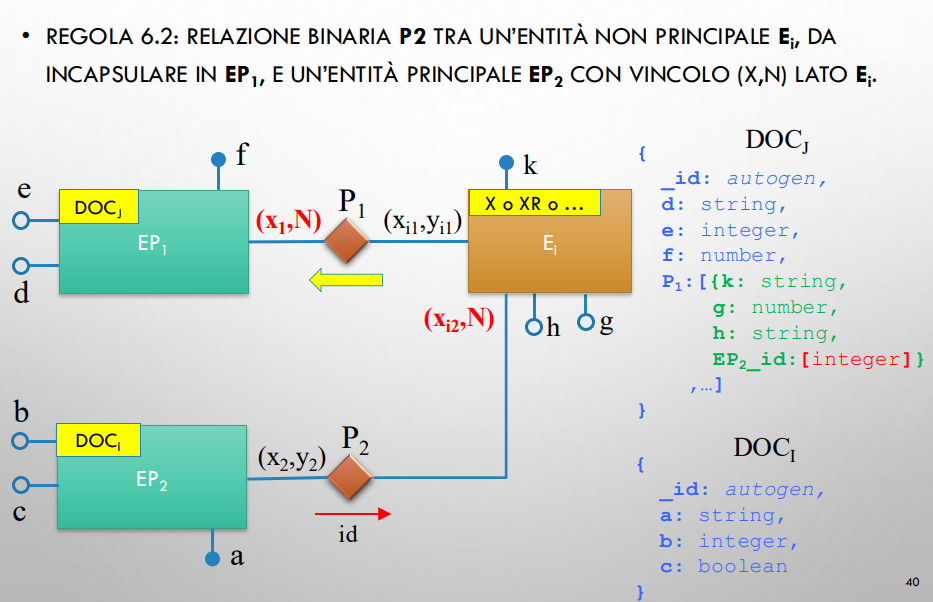
\includegraphics[width=1\linewidth]{image75.png}
\end{figure}

\begin{figure}[H]
\centering
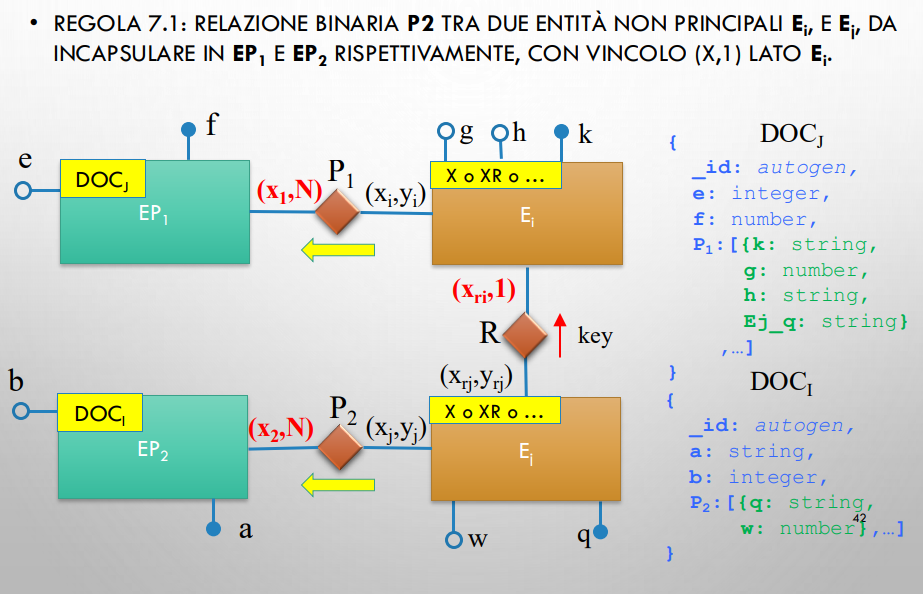
\includegraphics[width=1\linewidth]{image76.png}
\end{figure}

\begin{figure}[H]
\centering
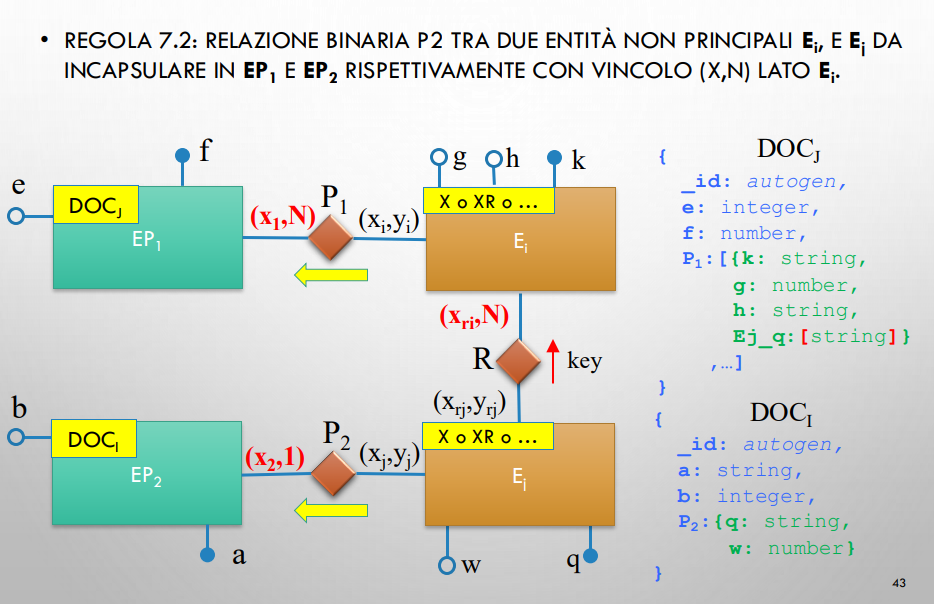
\includegraphics[width=1\linewidth]{image77.png}
\end{figure}

	\section{Algebra relazionale}

L'\textbf{algebra relazionale} è un linguaggio formale procedurale che
definisce un insieme di \textbf{operatori} applicabili a relazioni
(tabelle) e che producono come risultato \textbf{nuove relazioni}.
Essa costituisce il fondamento teorico dei linguaggi di interrogazione
dei database relazionali, come SQL.

Ogni operatore dell'algebra relazionale è \textbf{chiuso}, ovvero
restituisce sempre una relazione come risultato, permettendo la
composizione di più operatori in un'unica espressione.

La \textbf{segnatura} di un operatore descrive:
\begin{itemize}
	\item il numero di relazioni di input;
	\item l'eventuale presenza di parametri;
	\item il tipo del risultato prodotto.
\end{itemize}

Un \textbf{operatore unario} agisce su una singola relazione di input e
produce una relazione di output:

\[
Op_{\text{parametri}}(r_1) \;\rightarrow\; r_2
\]

dove:
\begin{itemize}
	\item $r_1$ è la relazione di input;
	\item $Op$ è l'operatore applicato;
	\item i \emph{parametri} specificano il comportamento dell'operatore;
	\item $r_2$ è la relazione risultante.
\end{itemize}

Un \textbf{operatore binario} agisce su due relazioni di input e produce
una nuova relazione:

\[
r_1 \; Op_{\text{parametri}} \; r_2 \;\rightarrow\; r_3
\]

dove:
\begin{itemize}
	\item $r_1$ e $r_2$ sono le relazioni di input;
	\item $Op$ è l'operatore binario;
	\item i \emph{parametri} definiscono le condizioni dell'operazione;
	\item $r_3$ è la relazione risultante.
\end{itemize}
\subsection{Classificazione degli operatori}

Gli operatori dell'algebra relazionale si classificano secondo due
criteri principali:

\subsubsection*{Classificazione funzionale}

\begin{itemize}
	\item Operatori insiemistici
	\item Operatori specifici
	\item Operatori di giunzione (join) tra relazioni
\end{itemize}

\subsubsection*{Classificazione in base alla derivabilità}

\begin{itemize}
	\item Operatori di base
	\item Operatori derivati
\end{itemize}
\subsection{Operatori insiemistici}

Poiché le relazioni sono insiemi di tuple, è naturale applicare ad esse
le operazioni dell'algebra degli insiemi.  
È tuttavia necessario ricordare che una relazione è un insieme di tuple
\textbf{omogenee}, cioè definite sullo stesso insieme di attributi
(stesso schema).

Di conseguenza, gli operatori insiemistici possono essere applicati
esclusivamente a relazioni che hanno \textbf{lo stesso schema}.

Dati due relazioni $r_1$ e $r_2$ definite sullo stesso schema $X$, si
definiscono i seguenti operatori:
\begin{figure}[H]
	\centering
	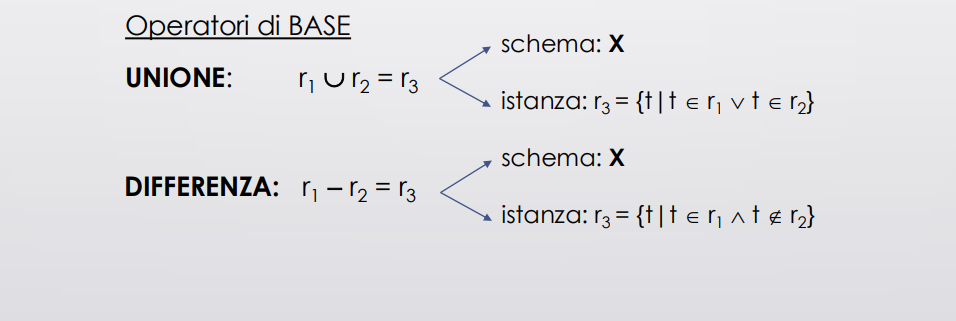
\includegraphics[width=1\linewidth]{image78}
	\caption{operazione di unione e differenza}
	\label{fig:image78}
\end{figure}
\begin{figure}[H]
	\centering
	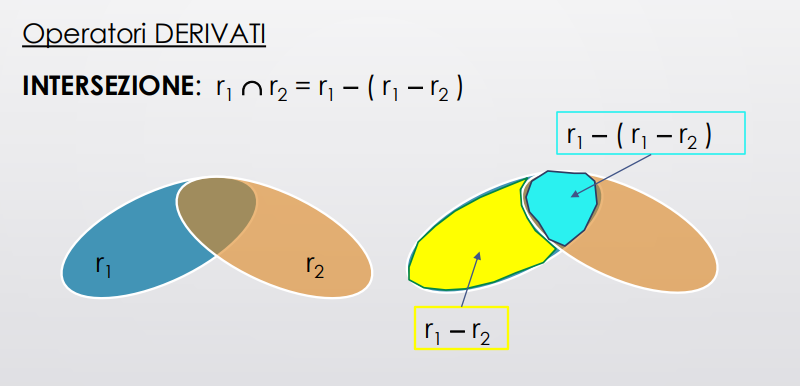
\includegraphics[width=1\linewidth]{image79}
	\caption{Intersezione}
	\label{fig:image79}
\end{figure}
\subsubsection{Cardinalità degli operatori insiemistici}

La \textbf{cardinalità} di una relazione indica il numero di tuple
contenute nella relazione risultante dall'applicazione di un operatore
dell'algebra relazionale.

\subsubsection*{Unione}

L'operatore di unione combina le tuple di due relazioni eliminando le
eventuali tuple duplicate.  
La cardinalità della relazione risultante dipende dal numero di tuple
comuni tra le due relazioni.

Il valore minimo si ottiene quando una relazione è interamente contenuta
nell'altra; in questo caso, la cardinalità dell'unione coincide con
quella della relazione più grande.  
Il valore massimo si ottiene quando le due relazioni non hanno tuple in
comune; in questo caso, la cardinalità dell'unione è pari alla somma
delle cardinalità delle due relazioni.

\[
\max(|r_1|, |r_2|) \;\le\; |r_1 \cup r_2| \;\le\; |r_1| + |r_2|
\]

\subsubsection*{Differenza}

L'operatore di differenza restituisce le tuple appartenenti alla prima
relazione che non sono presenti nella seconda relazione.  
La cardinalità della relazione risultante può variare da zero fino alla
cardinalità della prima relazione.

Il valore minimo si ottiene quando tutte le tuple della prima relazione
sono presenti anche nella seconda, producendo una relazione vuota.  
Il valore massimo si ottiene quando nessuna tupla della prima relazione è
presente nella seconda, per cui tutte le tuple della prima relazione
vengono mantenute.

\[
0 \;\le\; |r_1 - r_2| \;\le\; |r_1|
\]

\subsubsection*{Intersezione}

L'operatore di intersezione restituisce le tuple comuni a entrambe le
relazioni.  
La cardinalità della relazione risultante dipende quindi dal numero di
tuple condivise.

Il valore minimo si ottiene quando le due relazioni non hanno tuple in
comune, producendo una relazione vuota.  
Il valore massimo si ottiene quando la relazione più piccola è
interamente contenuta nella relazione più grande.

\[
0 \;\le\; |r_1 \cap r_2| \;\le\; \min(|r_1|, |r_2|)
\]
\subsection{Operatori specifici}
\subsubsection{Operatore di rinominaizone}
Dato una relazione $r$ definita sullo schema $X$, con
\[
X = \{A_1, \dots, A_n\},
\]
si definiscono i seguenti operatori.
L'operatore di \textbf{rinominazione} consente di modificare il nome degli
attributi di una relazione senza alterarne le tuple.  
Sia
\[
Y = \{B_1, \dots, B_n\}
\]
un insieme di attributi tale che $|Y| = |X|$.

La rinominazione è definita come:
\[
\rho_{A_1 \rightarrow B_1, \dots, A_n \rightarrow B_n}(r) = r_2
\]

dove:
\begin{itemize}
	\item lo schema della relazione risultante è $Y$;
	\item l'istanza $r_2$ contiene le stesse tuple di $r$;
	\item per ogni tupla $t \in r$ e per ogni $i \in \{1, \dots, n\}$,
	vale $t[B_i] = t[A_i]$.
\end{itemize}
\subsubsection*{Esempio}

Schema relazionale:
\begin{itemize}
	\item \texttt{CAPOLUOGO\_PROV(Nome, Popolazione, CAP)}
	\item \texttt{COMUNI\_MINORI(Nome, Abitanti, CAP)}
\end{itemize}

Per produrre la lista di tutti i comuni è necessario rendere compatibili
gli schemi delle due relazioni.  
Si applica quindi l'operatore di rinominazione per uniformare il nome
degli attributi:

\[
\rho_{\text{Popolazione} \rightarrow \text{Abitanti}}
(\text{CAPOLUOGO\_PROV}) \;\cup\; \text{COMUNI\_MINORI}
\]
Dato una relazione $r$ definita sullo schema $X$, con
\[
X = \{A_1, \dots, A_n\},
\]
si definiscono i seguenti operatori.
\subsubsection{Operatore di Selezione}
L'operatore di \textbf{selezione} consente di estrarre da una relazione le tuple
che soddisfano una determinata condizione.

La selezione è definita come:
\[
\sigma_F(r_1) = r_2
\]

dove:
\begin{itemize}
	\item lo schema della relazione risultante è lo stesso di $r_1$;
	\item l'istanza risultante è
	\[
	r_2 = \{\, t \mid t \in r_1 \land F(t) \,\};
	\]
	\item $F(t)$ indica che la tupla $t$ rende vera la formula $F$.
\end{itemize}

La formula $F(t)$ è una formula proposizionale ottenuta combinando,
mediante i connettivi logici $\land$, $\lor$ e $\neg$, condizioni
atomiche del tipo:
\[
A \; \theta \; B \quad \text{oppure} \quad A \; \theta \; c
\]

dove:
\begin{itemize}
	\item $A$ e $B$ sono attributi della relazione;
	\item $\theta \in \{=, \neq, >, \ge, <, \le\}$;
	\item $c$ è una costante appartenente al dominio di $A$ o compatibile
	con esso.
\end{itemize}

Una formula del tipo $A \; \theta \; B$ è vera sulla tupla $t$ se
$t[A] \; \theta \; t[B]$, mentre una formula del tipo
$A \; \theta \; c$ è vera se $t[A] \; \theta \; c$.

Le formule composte assumono valori booleani determinati dalle tavole di
verità dei connettivi logici utilizzati.
\subsubsection*{Esempio}

Schema relazionale:
\begin{itemize}
	\item \texttt{TRENO(Numero, PartOra, PartMin, Cat, Dest, ArrOra, ArrMin)}
	\item \texttt{FERMATA(NumTreno, Stazione, Ora, Min)}
\end{itemize}

Si richiede di produrre la lista di tutti i treni non regionali che
partono alle ore 12:00 o dopo le 12:00 e prima delle 16:00.

L'espressione in algebra relazionale è:
\[
\sigma_{\text{PartOra} \ge 12 \;\land\; \text{PartOra} < 16 \;\land\;
	\text{Cat} \neq \text{'REGIONALE'}}(\text{TRENO})
\]
\subsubsection{Proiezione}

L'operatore di proiezione consente di ridurre una relazione eliminando
alcuni attributi, mantenendo solo quelli di interesse.  
La riduzione avviene in senso verticale.

Sia $Y = \{A_1, \dots, A_m\} \subseteq X$ un sottoinsieme degli attributi
dello schema $X$ della relazione $r_1$.

La proiezione è definita come:
\[
\pi_Y(r_1) = r_2
\]

dove:
\begin{itemize}
	\item lo schema della relazione risultante è $Y$;
	\item l'istanza risultante è
	\[
	r_2 = \{\, t \mid \exists t' \in r_1 : t'[Y] = t \,\};
	\]
	\item $t'[Y]$ indica la tupla ottenuta da $t'$ considerando solo gli
	attributi appartenenti a $Y$;
	\item eventuali tuple duplicate vengono eliminate.
\end{itemize}
\subsubsection*{Esempio}

Schema relazionale:
\begin{itemize}
	\item \texttt{TRENO(Numero, PartOra, PartMin, Cat, Dest, ArrOra, ArrMin)}
	\item \texttt{FERMATA(NumTreno, Stazione, Ora, Min)}
\end{itemize}

Si richiede di estrarre il \textbf{numero} e l'\textbf{ora di partenza}
dei treni \textit{Freccia Rossa} (categoria = \texttt{'FR'}) con
destinazione \textit{Milano Centrale}.

L'espressione in algebra relazionale è:
\[
\pi_{\text{Numero}, \text{PartOra}}
\big(
\sigma_{\text{Dest} = \text{'Milano Centrale'} \;\land\;
	\text{Cat} = \text{'FR'}}
(\text{TRENO})
\big)
\]
\subsubsection{Cardinalità degli operatori specifici}

La cardinalità indica il numero di tuple contenute nella relazione risultato di un'operazione di algebra relazionale.

\paragraph{Selezione:}
L'operatore di selezione $\sigma$ filtra le tuple di una relazione in base a una condizione logica, senza modificare gli attributi.

La cardinalità della relazione risultante soddisfa la seguente relazione:
\[
0 \le |\sigma_F(r_1)| \le |r_1|
\]

Questo significa che:
\begin{itemize}
	\item la selezione può restituire nessuna tupla;
	\item può restituire tutte le tuple della relazione originale;
	\item non può mai aumentare il numero di tuple.
\end{itemize}

\paragraph{Proiezione}
L'operatore di proiezione $\Pi$ seleziona un sottoinsieme di attributi della relazione ed elimina eventuali tuple duplicate.

La cardinalità della relazione risultante è compresa tra:
\[
\min(|r_1|, 1) \le |\Pi_Y(r_1)| \le |r_1|
\]

In particolare:
\begin{itemize}
	\item la proiezione può ridurre il numero di tuple a causa dell'eliminazione dei duplicati;
	\item nel caso migliore, la cardinalità rimane invariata.
\end{itemize}

Se l'insieme di attributi $Y$ è una superchiave per la relazione $r_1$, allora non si generano duplicati e vale:
\[
|\Pi_Y(r_1)| = |r_1|
\]

\subsubsection{Operatori di giunzione (JOIN)}

Dati due relazioni $r_1$ e $r_2$ con schema rispettivamente $X_1$ e $X_2$, 
gli operatori di \textit{join} generano tuple nella relazione risultato 
a partire da coppie di tuple $(t_1, t_2) \in r_1 \times r_2$ che soddisfano 
una determinata condizione, detta \textit{predicato di join}.

\subsubsection{JOIN naturale}
Il join naturale è un operatore di base in cui il predicato di join è 
definito automaticamente sugli attributi comuni alle due relazioni.
Tale operatore è quindi dipendente dallo schema.

Lo schema della relazione risultante è:
\[
\text{schema}(r_3) = X_1 \cup X_2
\]

dove gli attributi comuni compaiono una sola volta.

L'istanza della relazione risultato è definita come:
\[
r_3 = \{\, t \mid \exists t_1 \in r_1,\ \exists t_2 \in r_2 :
t[X_1] = t_1 \land t[X_2] = t_2 \,\}
\]

Il predicato di join è una condizione di uguaglianza sugli attributi comuni
alle due relazioni.
\subsubsection*{Esempio}

Si consideri il seguente schema relazionale:

\[
\text{DOCENTE}(\underline{CFDocente}, Nome, Cognome)
\]
\[
\text{CORSO}(Nome, \underline{CFDocente})
\]

Si richiede di produrre l’insieme dei corsi riportando il nome del corso
e il cognome del docente che lo tiene.

Poiché le informazioni richieste sono distribuite su due relazioni
diverse, è necessario applicare un operatore di join.
Il collegamento tra le relazioni avviene tramite l’attributo comune
\texttt{CFDocente}.

Dal momento che l’attributo \texttt{Nome} della relazione \texttt{CORSO}
deve essere rinominato in \texttt{NomeCorso}, si applica preliminarmente
l’operatore di rinomina.

L’espressione di algebra relazionale è la seguente:

\[
\Pi_{NomeCorso,\, Cognome}
\Big(
\rho_{Nome \rightarrow NomeCorso}(\text{CORSO})
\;\bowtie\;
\text{DOCENTE}
\Big)
\]

L’operatore di join naturale combina le tuple delle due relazioni
sulla base dell’uguaglianza dell’attributo comune \texttt{CFDocente}.
Successivamente, la proiezione consente di ottenere esclusivamente
gli attributi richiesti nel risultato finale.

\begin{figure}[H]
	\centering
	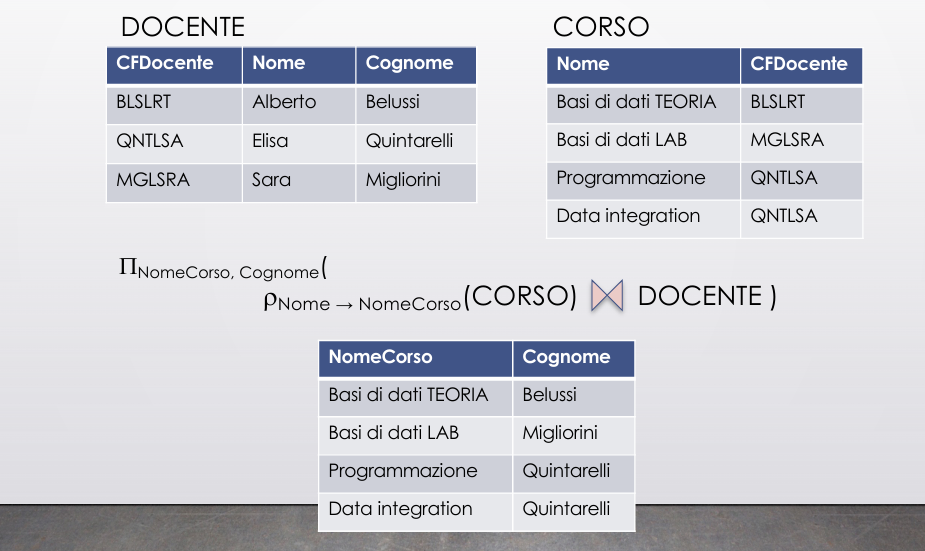
\includegraphics[width=1\linewidth]{image80}
	\caption{Esempio più visivo del JOIN naturale}
	\label{fig:image80}
\end{figure}
\subsubsection*{Proprietà del JOIN naturale}

Il join naturale tra due relazioni $r_1$ e $r_2$ si dice \emph{completo}
se tutte le tuple delle due relazioni contribuiscono a generare
almeno una tupla nella relazione risultato.

Formalmente, il join naturale è completo se valgono entrambe le seguenti
condizioni:

\[
\forall t_1 \in r_1:\ \exists t \in r_1 \bowtie r_2 \ \text{tale che} \ t[X_1] = t_1
\]

\[
\forall t_2 \in r_2:\ \exists t \in r_1 \bowtie r_2 \ \text{tale che} \ t[X_2] = t_2
\]

Queste condizioni garantiscono che ogni tupla di $r_1$ e di $r_2$
compaia almeno una volta nel risultato del join.

Se il join naturale non è completo, le tuple che non contribuiscono
alla generazione di alcuna tupla nel risultato si dicono
\textbf{dangling tuples}.
Il join naturale gode di alcune proprietà algebriche analoghe a quelle
degli operatori classici dell'algebra.

\paragraph{Commutatività:}
Il join naturale è commutativo:
\[
r_1 \bowtie r_2 = r_2 \bowtie r_1
\]

\paragraph{Associatività:}
Il join naturale è associativo:
\[
r_1 \bowtie (r_2 \bowtie r_3) = (r_1 \bowtie r_2) \bowtie r_3
\]

\paragraph{Relazioni con lo stesso schema:}
Se le relazioni $r_1$ e $r_2$ hanno lo stesso schema, allora il join
naturale coincide con l'intersezione:
\[
r_1 \bowtie r_2 = r_1 \cap r_2
\]

\paragraph{Assenza di attributi comuni:}
Se le relazioni $r_1$ e $r_2$ non hanno attributi in comune, allora il
join naturale coincide con il prodotto cartesiano:
\[
r_1 \bowtie r_2 = r_1 \times r_2
\]
\subsubsection{Cardinalità del JOIN naturale}
In generale, la cardinalità del join naturale tra due relazioni $r_1$ e $r_2$
è compresa tra zero e il prodotto delle cardinalità delle due relazioni:
\[
0 \le |r_1 \bowtie r_2| \le |r_1| \cdot |r_2|
\]

Se il join naturale è completo, allora ogni tupla di entrambe le relazioni
contribuisce a generare almeno una tupla nel risultato, e vale:
\[
\max(|r_1|, |r_2|) \le |r_1 \bowtie r_2| \le |r_1| \cdot |r_2|
\]

Se l’insieme degli attributi comuni $X_1 \cap X_2$ è una superchiave per
la relazione $r_2$, allora a ogni tupla di $r_1$ può corrispondere al più
una tupla di $r_2$, e quindi:
\[
0 \le |r_1 \bowtie r_2| \le |r_1|
\]

Se $X_1 \cap X_2$ è una superchiave per $r_2$ ed esiste un vincolo di
integrità referenziale tra $X_1 \cap X_2$ (o una sua parte) di $r_1$ e $r_2$,
allora ogni tupla di $r_1$ trova corrispondenza in $r_2$ e vale:
\[
|r_1 \bowtie r_2| = |r_1|
\]
\newpage
\subsubsection{THETA JOIN}
Date due relazioni \( r_1 \) e \( r_2 \) di schema \( X_1 \) e \( X_2 \) rispettivamente,
si introduce, oltre al \textit{join naturale}, il seguente operatore.
\textbf{Theta Join}: il predicato di join viene indicato esplicitamente
ed è indipendente dallo schema delle relazioni.

\subsubsection*{Precondizione}
Gli schemi delle relazioni devono essere disgiunti:
\[
X_1 \cap X_2 = \emptyset
\]


\subsubsection*{Definizione}
Il theta join è definito come una selezione applicata al prodotto cartesiano:
\[
r_1 \bowtie_\theta r_2 = \sigma_\theta ( r_1 \times r_2 )
\]

dove:
\begin{itemize}
	\item \( \times \) è il prodotto cartesiano
	\item \( \sigma_\theta \) è l’operatore di selezione
	\item \( \theta \) è un predicato conforme alla sintassi della selezione
\end{itemize}

Il predicato \( \theta \) può contenere confronti tra attributi delle due relazioni
utilizzando operatori di confronto come \( =, \neq, <, >, \leq, \geq \).

\begin{figure}[H]
	\centering
	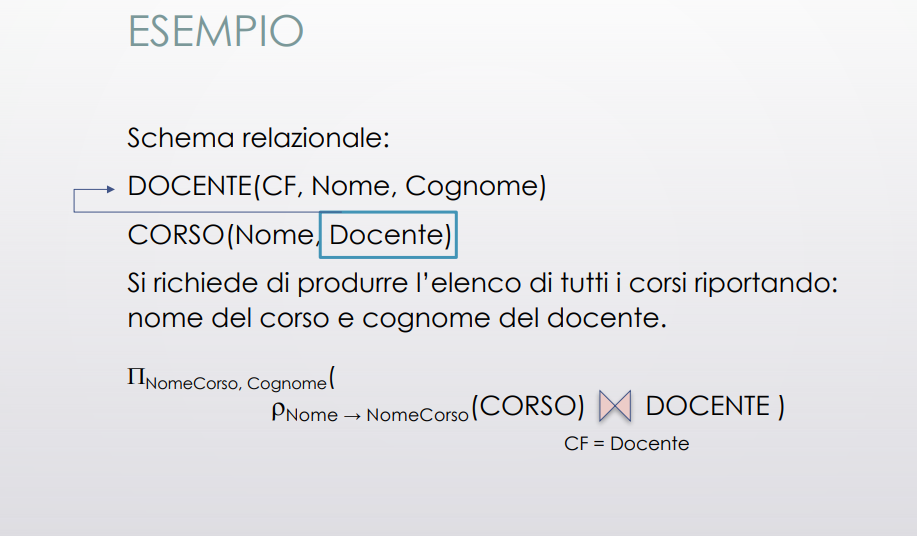
\includegraphics[width=1\linewidth]{image81}
	\caption{Esempio dell'uso del Theta Join}
	\label{fig:image81}
\end{figure}
\subsection*{Proprietà del Theta Join}

Il \textbf{theta join} si dice \textbf{equi-join} se la condizione
\( \theta \) è una congiunzione di uguaglianze:

\[
r_1 \;\bowtie_{\;A_1 = B_1 \;\wedge\; \dots \;\wedge\; A_n = B_n}\; r_2
\]

\bigskip

\noindent
\textbf{N.B.:} \textbf{ATTENZIONE} non esiste un operatore misto che applica
la logica del \emph{join naturale} per gli attributi comuni e aggiunge
ulteriori condizioni specificate esplicitamente tramite il predicato
\( \theta \).\\
\textbf{Teorema}

Date due relazioni \( r_1 \) e \( r_2 \) di schema \( X_1 \) e \( X_2 \) con
\[
X_1 \cap X_2 = \{ C_1, \dots, C_m \} \quad \text{con } m > 0,
\]
vale la seguente equivalenza:

\[
r_1 \bowtie r_2
=
\Pi_{X_1 \cup X_2}
\left(
r_1
\;\bowtie_{\;C_1 = C'_1 \;\wedge\; \dots \;\wedge\; C_m = C'_m}\;
\rho_{C_1, \dots, C_m \rightarrow C'_1, \dots, C'_m}(r_2)
\right)
\]


\paragraph{Ridenominazione}
Data la relazione \( r_1 \) di schema
\[
X_1 = \{ A_1, \dots, A_n \},
\]
per cambiare nome a tutti gli attributi si può scrivere:

\[
\rho_{A_1, \dots, A_n \rightarrow A'_1, \dots, A'_n}(r_1)
\]

oppure, in forma breve:

\[
\rho_{X \rightarrow X'}(r_1)
\]

\bigskip

\noindent
\textbf{N.B.:} \textbf{non sono ammesse} notazioni simili alla \emph{dot notation}
per indicare l’attributo di una tabella.

\noindent
La notazione \( T.A \) (per indicare l’attributo \( A \) della tabella \( T \))
\textbf{NON è una notazione ammessa dall’algebra relazionale}.
\subsection{Algebra con valori nulli}
È opportuno estendere l’algebra relazionale affinché possa operare anche su relazioni che contengono valori nulli.
In particolare, è necessario definire in modo esplicito il comportamento delle operazioni che coinvolgono il
confronto tra attributi, poiché la presenza di valori nulli introduce ambiguità semantiche.

Le operazioni che richiedono una gestione specifica dei valori nulli sono:
\begin{itemize}
	\item \textbf{Selezione}
	\item \textbf{Join naturale}
\end{itemize}

Le altre operazioni dell’algebra relazionale (proiezione, unione, differenza e prodotto cartesiano) 
si limitano a propagare i valori nulli eventualmente presenti nelle tuple di input, senza introdurre
nuove problematiche semantiche.

\medskip

\noindent
\textbf{Motivazione:}
La selezione e il join naturale si basano su confronti tra valori di attributi.
In presenza di valori nulli, tali confronti non possono essere valutati secondo la logica booleana classica,
ma richiedono una logica a tre valori (\textit{vero}, \textit{falso}, \textit{sconosciuto}).
Per questo motivo, è necessario estendere formalmente l’algebra relazionale per garantire
un comportamento coerente e ben definito di queste operazioni.
\subsubsection{Selezione}

Le condizioni di selezione in presenza di valori nulli assumono i seguenti valori di verità:

\begin{itemize}
	\item Sia $A \,\theta\, B$ una condizione atomica applicata a una tupla $t$.
	Se $t[A] = \text{NULL}$ oppure $t[B] = \text{NULL}$, allora l’espressione
	$t[A] \,\theta\, t[B]$ è valutata come \textbf{FALSO}.
	
	\item Sia $A \,\theta\, c$ una condizione atomica applicata a una tupla $t$, dove $c$ è una costante.
	Se $t[A] = \text{NULL}$, allora l’espressione
	$t[A] \,\theta\, c$ è valutata come \textbf{FALSO}.
	
	\item Sono introdotte le seguenti condizioni atomiche aggiuntive:
	\[
	A \ \text{IS NULL} \qquad \text{e} \qquad A \ \text{IS NOT NULL}.
	\]
	L’espressione $A \ \text{IS NULL}$, valutata sulla tupla $t$, è \textbf{VERO} se $t[A] = \text{NULL}$,
	altrimenti è \textbf{FALSO}.  
	Viceversa, l’espressione $A \ \text{IS NOT NULL}$ è \textbf{VERO} se $t[A] \neq \text{NULL}$,
	altrimenti è \textbf{FALSO}.
\end{itemize}
\subsubsection{Join naturale}

Nel join naturale, la condizione di uguaglianza sugli attributi comuni alle due relazioni
è valutata come \textbf{FALSA} sulle tuple $t_1$ e $t_2$ se almeno uno degli attributi comuni
di $t_1$ oppure di $t_2$ assume valore \texttt{NULL}.

\medskip

Si osservi, in particolare, che il confronto
\[
\texttt{NULL} = \texttt{NULL}
\]
è sempre valutato come \textbf{FALSO}.
\subsection{Ottimizzazione di espressioni DML}
Ogni espressione DML (generalmente specificata tramite un linguaggio dichiarativo)
ricevuta dal DBMS è sottoposta a un processo di elaborazione e ottimizzazione
prima della sua esecuzione.

\begin{figure}[H]
	\centering
	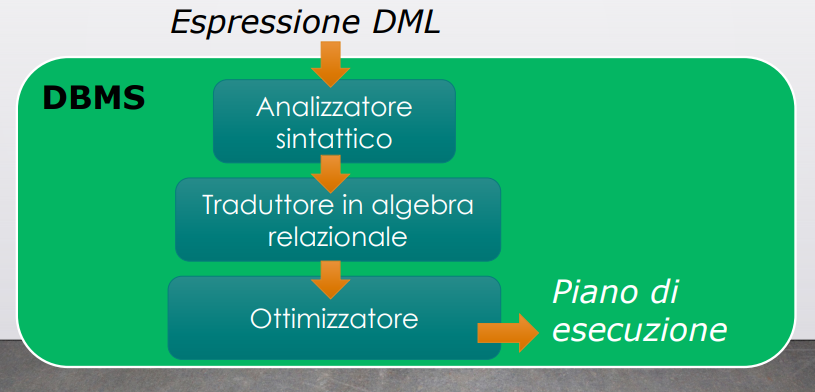
\includegraphics[width=\linewidth]{image82}
	\caption{Ottimizzazione di espressioni DML}
	\label{fig:image82}
\end{figure}

L’ottimizzatore genera un’espressione equivalente a quella di input, ma caratterizzata
da un costo inferiore.
Il costo viene stimato principalmente in termini di dimensione dei risultati intermedi,
numero di accessi ai dati e operazioni eseguite.

\medskip

Per ridurre il costo complessivo dell’esecuzione, l’ottimizzatore applica
trasformazioni di equivalenza sull’espressione di input,
con l’obiettivo di minimizzare la dimensione dei risultati intermedi e migliorare
l’efficienza dell’elaborazione.
\subsection{Equivalenza tra espressioni algebriche}

\subsubsection{Equivalenza dipendente dallo schema}

Dato uno schema $R$, due espressioni algebriche $E_1$ ed $E_2$ si dicono
\emph{equivalenti rispetto allo schema $R$}, e si scrive:
\[
E_1 \equiv_R E_2
\]
se vale che
\[
E_1(r) = E_2(r) \quad \text{per ogni istanza } r \text{ dello schema } R.
\]

\medskip

\noindent
\textbf{Esempio:}
\[
\Pi_{AB}(R_1) \;\bowtie\; \Pi_{AC}(R_2)
\;\equiv_R\;
\Pi_{ABC}(R_1 \;\bowtie\; R_2)
\]

\subsubsection{Equivalenza assoluta}

L’equivalenza assoluta è indipendente dallo schema.
Due espressioni $E_1$ ed $E_2$ si dicono \emph{assolutamente equivalenti}, e si scrive:
\[
E_1 \equiv E_2
\]
se vale che
\[
E_1 \equiv_R E_2 \quad \text{per ogni schema } R \text{ compatibile con } E_1 \text{ ed } E_2.
\]

\medskip

\noindent
\textbf{Esempio:}
\[
\Pi_{AB}(\sigma_{A>0}(R)) \;\equiv\; \sigma_{A>0}(\Pi_{AB}(R))
\]

% --------------------------------------------------

\subsection{Trasformazioni di equivalenza}

Sia $E$ un’espressione di schema $X$. Si definiscono le seguenti trasformazioni
di equivalenza.

\subsubsection*{Atomizzazione delle selezioni}

\[
\sigma_{F_1 \land F_2}(E) \;\equiv\; \sigma_{F_1}(\sigma_{F_2}(E))
\]

Questa trasformazione è propedeutica ad altre trasformazioni.
Da sola non produce un’ottimizzazione se non è seguita da ulteriori riscritture.

\subsubsection{Idempotenza delle proiezioni}

\[
\Pi_Y(E) \;\equiv\; \Pi_Y(\Pi_Z(E)) \qquad \text{con } Z \subseteq X
\]

Anche questa trasformazione è propedeutica e non comporta
un’ottimizzazione se applicata isolatamente.

% --------------------------------------------------

\subsection{Trasformazioni di equivalenza con il join}

Siano $E_1$ ed $E_2$ espressioni di schema rispettivamente $X_1$ e $X_2$.

\subsubsection*{Anticipazione delle selezioni rispetto al join}

\[
\sigma_F(E_1 \bowtie E_2) \;\equiv\; E_1 \bowtie \sigma_F(E_2)
\]

La trasformazione è applicabile solo se la condizione $F$ fa riferimento
esclusivamente ad attributi di $E_2$.

\subsubsection*{Anticipazione della proiezione rispetto al join}

\[
\Pi_{X_1 \cup Y}(E_1 \bowtie E_2) \;\equiv_R\; E_1 \bowtie \Pi_Y(E_2)
\]


La trasformazione è applicabile solo se:
\[
Y \subseteq X_2
\quad \mbox{e} \quad
(X_2 - Y) \cap X_1 = \emptyset
\]

% --------------------------------------------------

\subsection{Combinazione di anticipazione e idempotenza}

Combinando l’anticipazione della proiezione con l’idempotenza delle proiezioni
si ottengono le seguenti equivalenze:

\[
\Pi_Y(E_1 \bowtie_F E_2)
\;\equiv\;
\Pi_Y\bigl(\Pi_{Y_1}(E_1) \bowtie_F \Pi_{Y_2}(E_2)\bigr)
\]


\[
\Pi_Y(E_1 \bowtie E_2)
\;\equiv\;
\Pi_Y\bigl(\Pi_{Y_1}(E_1) \bowtie \Pi_{Y_2}(E_2)\bigr)
\]

dove:
\begin{itemize}
	\item $Y_1 = (X_1 \cap Y) \cup J_1$
	\item $Y_2 = (X_2 \cap Y) \cup J_2$
	\item $J_1$ e $J_2$ sono gli attributi di $E_1$ ed $E_2$ coinvolti nel join.
	Nel caso di theta-join, tali attributi sono quelli presenti nella condizione $F$;
	nel caso di join naturale vale:
	\[
	J_1 = J_2 = X_1 \cap X_2
	\]
\end{itemize}
\begin{figure}[H]
	\centering
	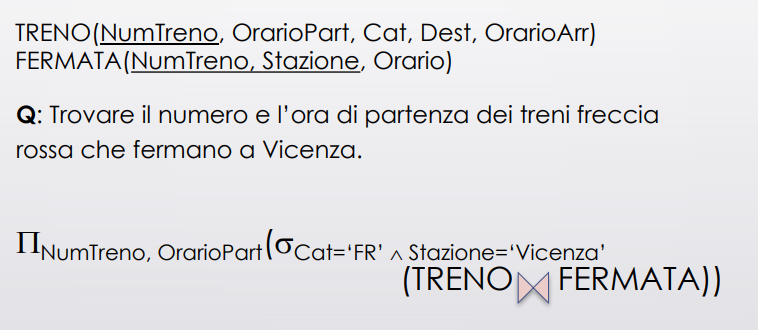
\includegraphics[width=1\linewidth]{image83}
	\caption[]{Esempio di applicazione delle trasformazioni}
	\label{fig:image83}
\end{figure}
\begin{figure}[H]
	\centering
	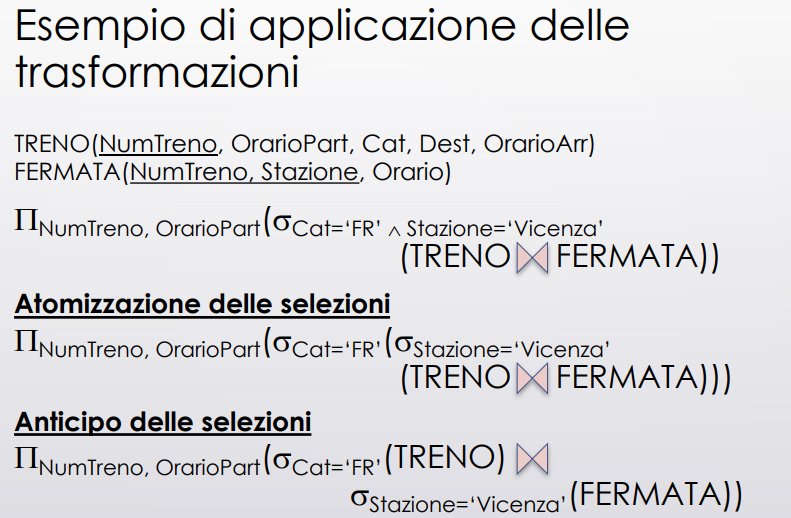
\includegraphics[width=1\linewidth]{image84}
	\caption[]{Esempio di applicazione delle trasformazioni}
	\label{fig:image84}
\end{figure}
\begin{figure}[H]
	\centering
	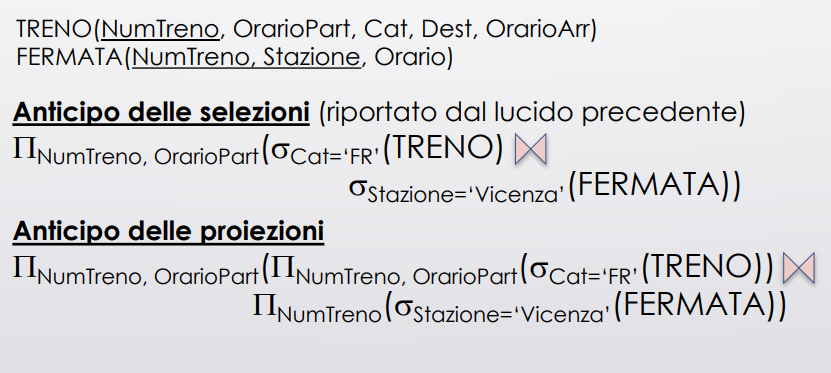
\includegraphics[width=1\linewidth]{image85}
	\caption{Esempio di applicazione delle trasformazioni}
	\label{fig:image85}
\end{figure}
\subsection*{Ulteriori trasformazioni di equivalenza}

Siano $E_1$ ed $E_2$ espressioni di schema rispettivamente $X_1$ e $X_2$.
Si definisce la seguente trasformazione di equivalenza.

\subsubsection*{Inglobamento di una selezione in un prodotto cartesiano}

Questa trasformazione consente di inglobare una selezione applicata a un prodotto
cartesiano in un join con condizione:

\[
\sigma_F(E_1 \times E_2) \;\equiv\; E_1 \bowtie_F E_2
\]

La trasformazione è applicabile solo se:
\[
X_1 \cap X_2 = \emptyset
\]

\noindent
Si osservi che questa regola va applicata solo dopo aver verificato che non sia
possibile anticipare le selezioni rispetto al join.

\begin{figure}[H]
	\centering
	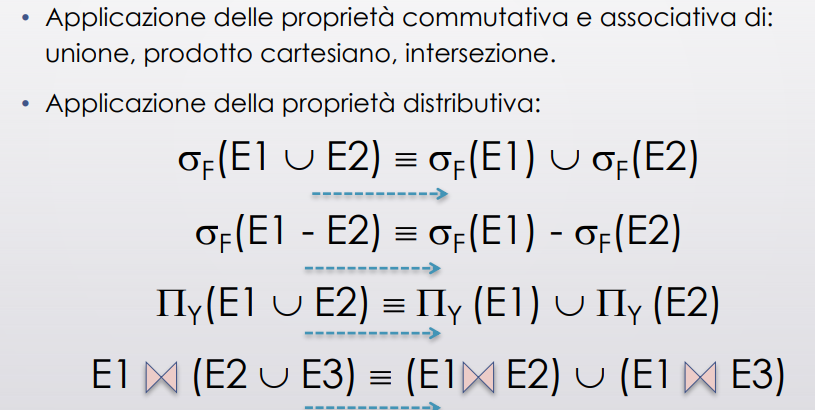
\includegraphics[width=1\linewidth]{image86}
	\caption{Applicazione della proprietà distributiva}
	\label{fig:image86}
\end{figure}
\begin{figure}[H]
	\centering
	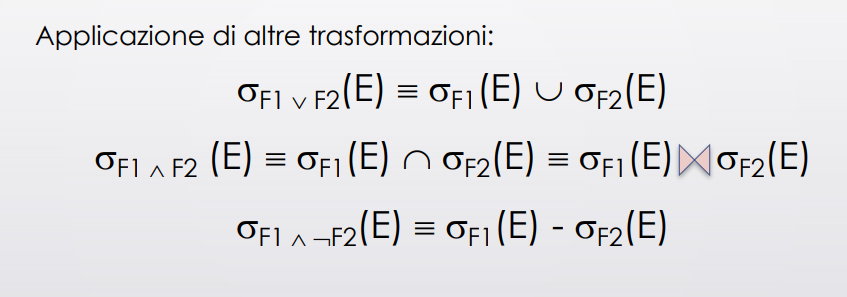
\includegraphics[width=1\linewidth]{image87}
	\caption{applicazione di altre trasformazioni}
	\label{fig:image87}
\end{figure}
\begin{figure}[H]
	\centering
	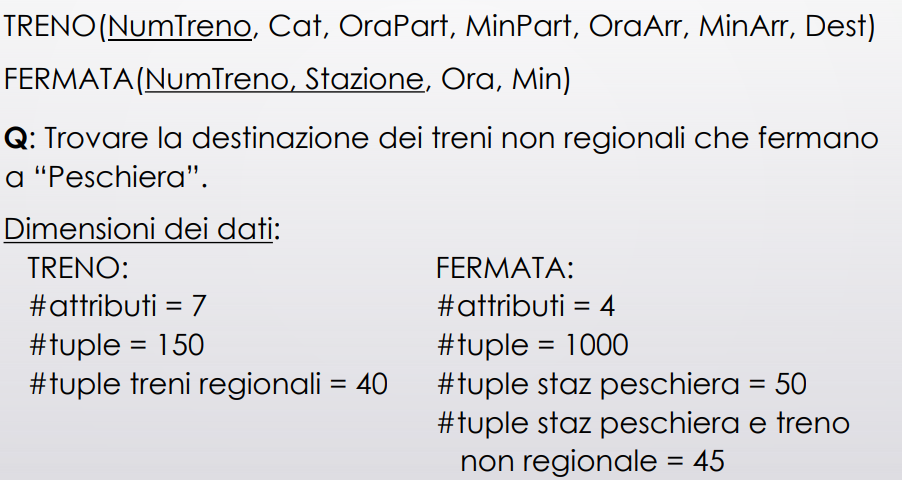
\includegraphics[width=1\linewidth]{image88}
	\caption{Esempio}
	\label{fig:image88}
\end{figure}


	\section{Calcolo Relazionale}
Il calcolo relazionale è un linguaggio di interrogazione dichiarativo: esso specifica le proprietà che devono essere soddisfatte dal risultato dell’interrogazione, senza descrivere le modalità operative per ottenerlo.

Esistono due versioni del calcolo relazionale:
\begin{itemize}
	\item il calcolo relazionale sui domini;
	\item il calcolo relazionale sulle tuple.
\end{itemize}

\paragraph{Caratteristiche del linguaggio}
Nel calcolo relazionale sulle tuple, un’interrogazione è specificata mediante una formula logica con variabili libere.  
La formula viene interpretata sul contenuto della base di dati e le variabili assumono come valori le tuple delle relazioni presenti nella base di dati.

Il calcolo relazionale sulle tuple costituisce il fondamento teorico del linguaggio SQL nella sua forma \emph{semplice}, ossia senza operatori aggregati e senza join esterni, includendo le interrogazioni nidificate.

\begin{figure}[H]
	\centering
	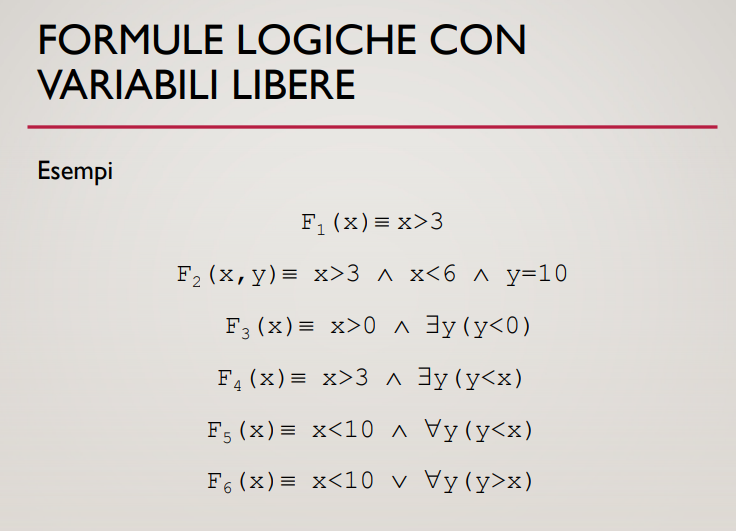
\includegraphics[width=1\linewidth]{image89}
	\caption{Esempi di formule logiche con variabili libere}
	\label{fig:image89}
\end{figure}
\paragraph{Interpretazione}
L’interpretazione consiste nella scelta degli insiemi da cui prelevare i valori da assegnare alle variabili.
Ad esempio, una formula può essere interpretata sull’insieme degli interi $\mathbb{Z}$ oppure sull’insieme dei numeri naturali $\mathbb{N}$.
\begin{figure}[H]
	\centering
	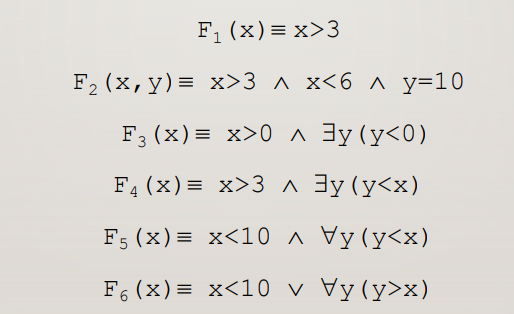
\includegraphics[width=1\linewidth]{image90}
	\caption{Formule logiche con variabili libere}
	\label{fig:image90}
\end{figure}
\paragraph{Sintassi}
Le espressioni del calcolo relazionale sulle tuple hanno la seguente forma:
\[
\{\, T \mid L \mid F \,\}
\]
dove:
\begin{itemize}
	\item \textbf{Target list} ($T$): definisce lo schema della relazione risultato e specifica come le tuple del risultato sono ottenute a partire dalle variabili libere.
	
	\item \textbf{Range list} ($L$): definisce le variabili libere e le associa alle relazioni della base di dati coinvolte nell’interrogazione.
	
	\item \textbf{Formula} ($F$): specifica la condizione logica che deve essere soddisfatta dalle variabili libere, ossia dalle tuple coinvolte nell’interrogazione.
\end{itemize}
\subsection{Sintassi}
\paragraph{Sintassi Target List}
La \textbf{target list} $T$ è una lista di elementi separati da virgole:
\[
e_1, \ldots, e_n
\]

dove ogni elemento $e_i$ può essere:
\begin{itemize}
	\item $Y : x.(Z)$,  
	dove $Y$ e $Z$ sono sequenze di attributi con la stessa cardinalità e $x$ è una variabile libera.
	
	\item $x.(Z)$,  
	dove $Z$ è una sequenza di attributi e $x$ è una variabile libera (equivalente a $Z : x.(Z)$).
	
	\item $x.*$,  
	dove $x$ è una variabile libera; in questo caso gli attributi sono tutti quelli della relazione associata alla variabile $x$ nella \emph{range list} $L$.
\end{itemize}
\paragraph{Sintassi range list}
La \textbf{range list} $L$ è una lista di elementi separati da virgole:
\[
r_1, \ldots, r_m
\]

dove ogni elemento $r_i$ ha la seguente forma:
\[
x_j(R)
\]

dove $x_j$ è una variabile libera e $R$ è il nome di una relazione dello schema della base di dati.

Per ogni variabile libera della formula $F$ esiste uno e un solo elemento $r_i$ nella \emph{range list} $L$.
\paragraph{Sintassi della formula}
La formula $F$ può essere:

\paragraph{Formula atomica}
\begin{itemize}
	\item $x.A \ \theta \ c$ \quad oppure
	\item $x_1.A_1 \ \theta \ x_2.A_2$
\end{itemize}

dove $x, x_1, x_2$ sono variabili, $A, A_1, A_2$ sono attributi, $c$ è una costante e $\theta$ è un operatore di confronto appartenente all’insieme:
\[
\{=, \neq, >, <, \geq, \leq\}.
\]

\paragraph{Formula non atomica}
\begin{itemize}
	\item se $f_1$ e $f_2$ sono formule, allora anche
	\[
	f_1 \land f_2,\quad f_1 \lor f_2,\quad \neg f_1,\quad \neg f_2
	\]
	sono formule;
	
	\item se $f$ è una formula, allora anche
	\[
	\forall x(R)\,(f) \quad \text{e} \quad \exists x(R)\,(f)
	\]
	sono formule.
\end{itemize}
\paragraph{Notazione} Variabili libere e legate nelle formule:
\begin{itemize}
	\item Nelle formule atomiche tutte le variabili sono libere.
	\item Nelle formule $\forall x\, (f)$ e $\exists x\, (f)$, la variabile $x$ è una variabile legata, mentre tutte le altre variabili mantengono lo stato (libere o legate) che avevano in $f$.
	\item Le congiunzioni, le disgiunzioni e la negazione non modificano l’insieme delle variabili libere o legate di una formula.
\end{itemize}
\subsection{Semantica}
\paragraph{Semantica}
Le formule vengono interpretate sull’istanza corrente della base di dati
\[
\mathit{db} = \{ r_1(x_1,\dots,x_n), \dots, r_m(x_1,\dots,x_n) \}.
\]
Ogni formula contiene un certo numero di variabili libere
\[
f(x_1,\dots,x_k).
\]
Data una ennupla di tuple $(t_1,\dots,t_k)$, tale ennupla rende vera la formula
quando, sostituendo le tuple $t_1,\dots,t_k$ alle variabili libere
$x_1,\dots,x_k$, la formula risulta soddisfatta.

Nel caso delle formule atomiche, una formula del tipo
\[
x_{i,A} \,\theta\, x_{j,B}
\]
è vera sulle tuple $(t_1,\dots,t_k)$ se il confronto
$t_{i,A} \,\theta\, t_{j,B}$ è soddisfatto; analogamente,
\[
x_{i,A} \,\theta\, c
\]
è vera se il confronto $t_{i,A} \,\theta\, c$ è soddisfatto, dove $\theta$ è un
operatore di confronto.

Le formule non atomiche ottenute mediante i connettivi logici
$\wedge$, $\vee$, $\neg$, $\Rightarrow$ sono vere secondo le usuali definizioni
di verità dei connettivi logici.

Per quanto riguarda i quantificatori, la formula
\[
\exists x_k\, (f)
\]
è vera sulle tuple $(t_1,\dots,t_{k-1})$ se esiste almeno una tupla $t_k$
nell’istanza di $R_k$ tale che, sostituendo $(t_1,\dots,t_k)$ alle variabili
$(x_1,\dots,x_k)$, la formula $f$ risulta vera.
Analogamente, la formula
\[
\forall x_k\, (f)
\]
è vera sulle tuple $(t_1,\dots,t_{k-1})$ se per ogni tupla $t_k$ nell’istanza di
$R_k$ la formula $f$ risulta vera quando si sostituiscono le tuple
$(t_1,\dots,t_k)$ alle variabili $(x_1,\dots,x_k)$.
\paragraph{Interpretazione di un’espressione del calcolo come interrogazione}
Un’espressione del calcolo relazionale sulle tuple può essere interpretata come
un’interrogazione della forma
\[
Q = \{\, Y_1 : x_1(Z_1), \dots, Y_k : x_k(Z_k)
\mid x_1(R_1), \dots, x_n(R_n) \mid f(x_1,\dots,x_n) \,\}.
\]

La valutazione dell’interrogazione $Q$ produce una relazione risultato $R$ tale che:
\begin{itemize}
	\item lo schema di $R$ è
	\[
	Y = Y_1 \cup \dots \cup Y_k;
	\]
	\item $R$ contiene tutte le tuple $t$ su $Y$ per le quali esiste una ennupla di
	tuple
	\[
	(t_1,\dots,t_n) \in R_1 \times \dots \times R_n
	\]
	che genera $t$ e che, sostituita alle variabili libere
	$(x_1,\dots,x_n)$, rende vera la formula $f$.
\end{itemize}
\subsection{Calcolo relazionale sulle tuple}
Il calcolo relazionale sulle tuple non è equivalente né all’algebra relazionale
né al calcolo relazionale sui domini, in quanto l’operatore di unione tra due
relazioni non è esprimibile nel calcolo relazionale sulle tuple.
Tuttavia, nel calcolo relazionale sulle tuple è possibile rappresentare sia
l’intersezione sia la differenza tra due relazioni.
\begin{figure}[H]
	\centering
	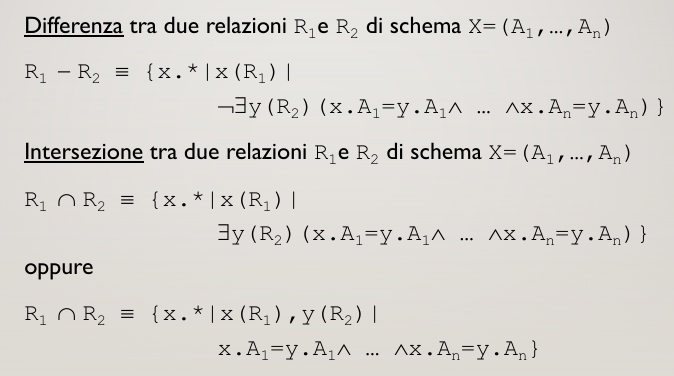
\includegraphics[width=1\linewidth]{image91}
	\caption{differenza e intersezione}
	\label{fig:image91}
\end{figure}
\begin{figure}[H]
	\centering
	
\includegraphics[width=1\linewidth]{image92}
	\caption{unione}
	\label{fig:image92}
\end{figure}
\subsection*{Esempio}
\begin{figure}[H]
	\centering
	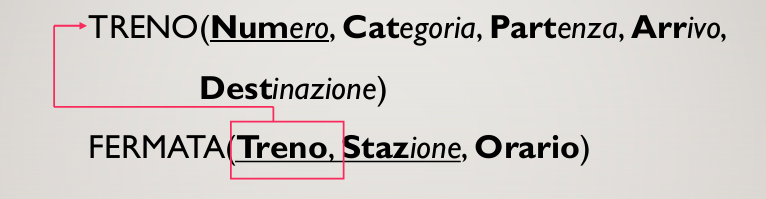
\includegraphics[width=1\linewidth]{image93}
	\caption{Progettazione Logica}
	\label{fig:image93}
\end{figure}
\begin{figure}[H]
	\centering
	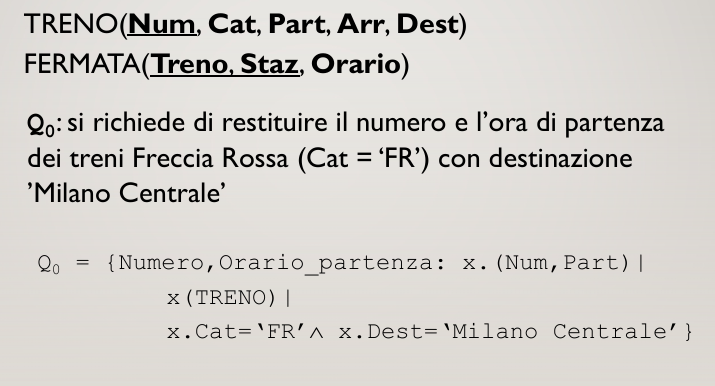
\includegraphics[width=1\linewidth]{image94}
	\caption{$Q_0$}
	\label{fig:image94}
\end{figure}
\begin{figure}[H]
	\centering
	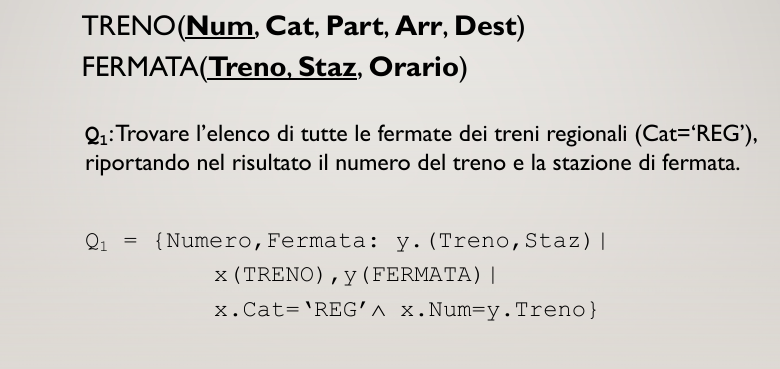
\includegraphics[width=1\linewidth]{image95}
	\caption{$Q_1$}
	\label{fig:image95}
\end{figure}

\begin{figure}[H]
	\centering
	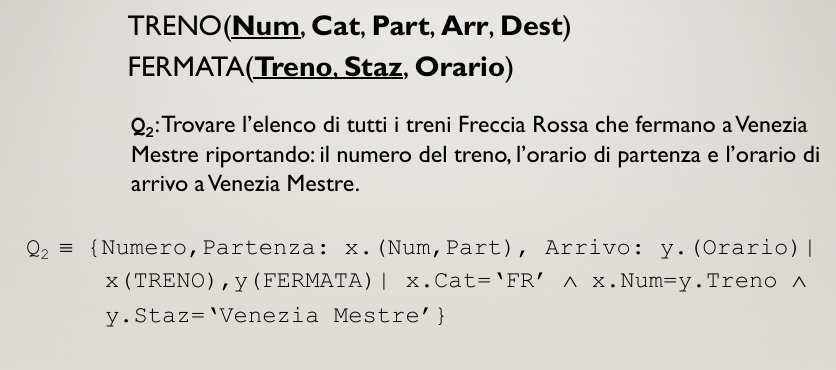
\includegraphics[width=1\linewidth]{image96}
	\caption{$Q_2$}
	\label{fig:image96}
\end{figure}
% TODO: \usepackage{graphicx} required
\begin{figure}[H]
	\centering
	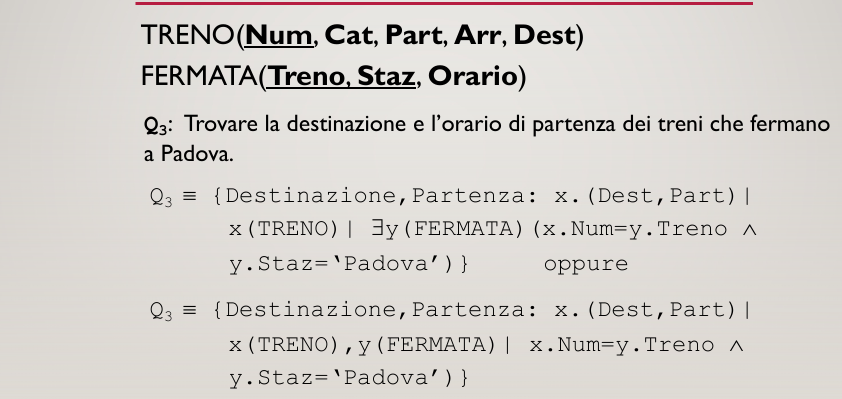
\includegraphics[width=1\linewidth]{image97}
	\caption{$Q_3$}
	\label{fig:image97}
\end{figure}
% TODO: \usepackage{graphicx} required
\begin{figure}[H]
	\centering
	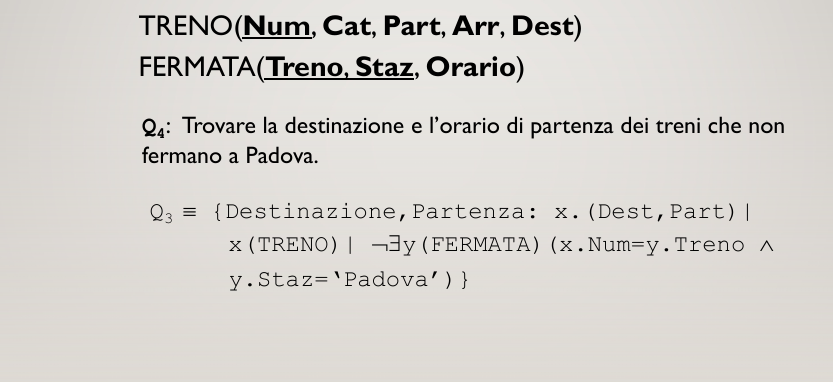
\includegraphics[width=1\linewidth]{image98}
	\caption{$Q_4$}
	\label{fig:image98}
\end{figure}
Il calcolo relazionale sulle tuple è equivalente al linguaggio di interrogazione
adottato dallo standard SQL2, se si considera la forma base delle interrogazioni
SQL, ovvero senza l’uso di operatori aggregati e di raggruppamenti.
In tale contesto, ogni espressione del calcolo relazionale sulle tuple è
direttamente traducibile in una interrogazione SQL di base.

In particolare, un’espressione del calcolo della forma
\[
\{\, T \mid L \mid F \,\}
\]
è in diretta corrispondenza con la forma base delle interrogazioni SQL:
\[
\texttt{SELECT } T \;\texttt{ FROM } L \;\texttt{ WHERE } F.
\]

La \emph{target list} $T$ individua gli attributi da restituire nel risultato
dell’interrogazione ed è mappata sulla clausola \texttt{SELECT};
la \emph{range list} $L$ specifica le relazioni coinvolte ed è mappata sulla
clausola \texttt{FROM};
infine, la formula $F$ esprime le condizioni di selezione ed è mappata sulla
clausola \texttt{WHERE}.

	\section{Linguaggi di interrogazione nei sistemi NoSql}
Nei sistemi NoSqlspesso non sono disponibili veri e propri linguaggi di interrogazione come nei sistemi relazionali.
Solo i sistemi document-based forniscono strumenti simili all'algebra e al calcolo relazionale per l'accesso ai dati.
\begin{figure}[H]
	\centering
	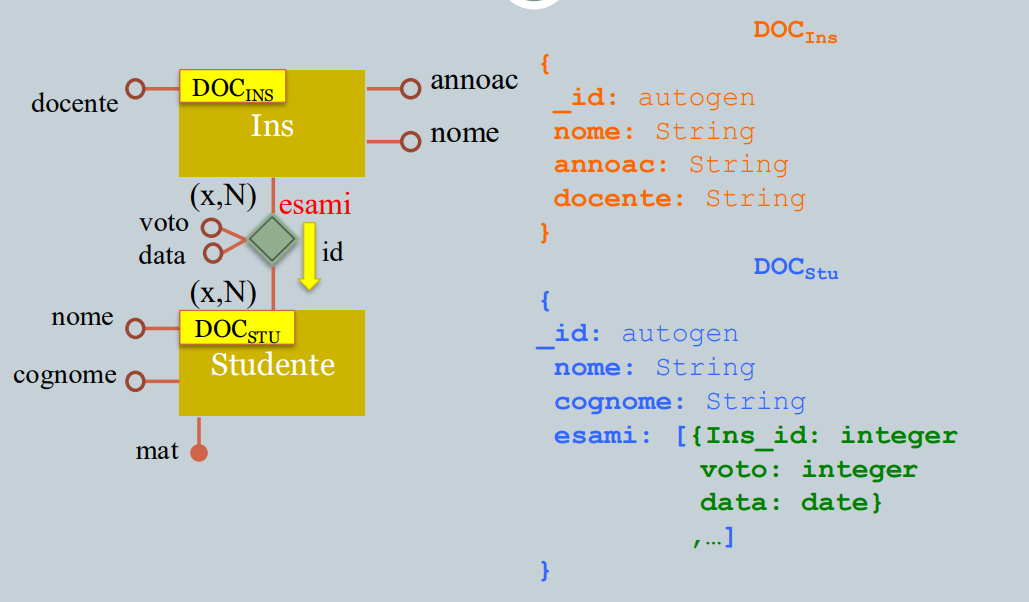
\includegraphics[width=1\linewidth]{image99}
	\caption{esempio sistemi document-store}
	\label{fig:image99}
\end{figure}
La maggior parte del linguaggio di interrogazione di MongoDB è realizzato attraverso il metodo find.
\begin{figure}[H]
	\centering
	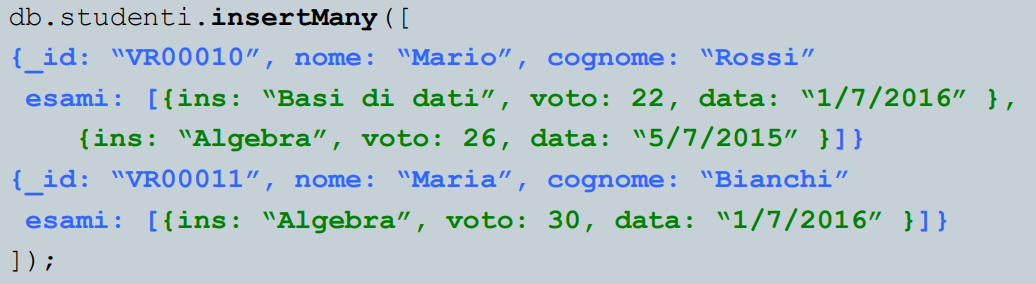
\includegraphics[width=1\linewidth]{image100}
	\caption{esempio con mongo db del document based di prima}
	\label{fig:image100}
\end{figure}
\begin{figure}[H]
	\centering
	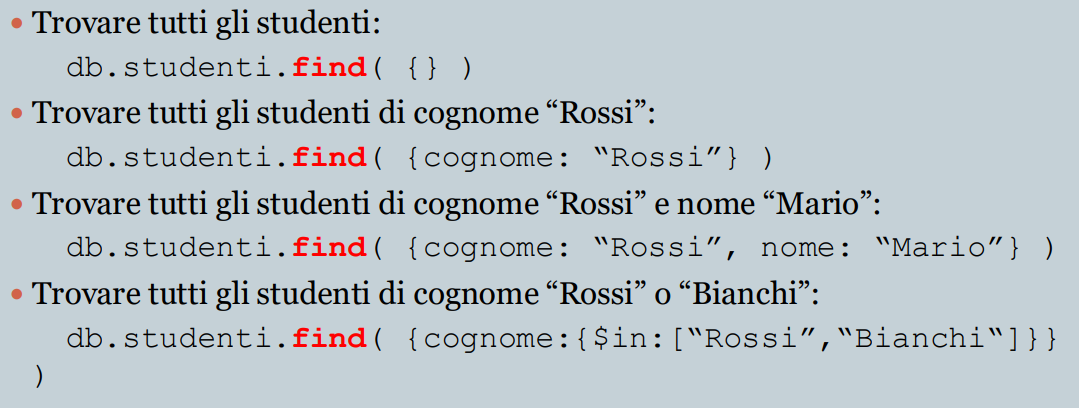
\includegraphics[width=1\linewidth]{image101}
	\caption{Interrogazioni Semplici}
	\label{fig:image101}
\end{figure}
\begin{figure}[H]
	\centering
	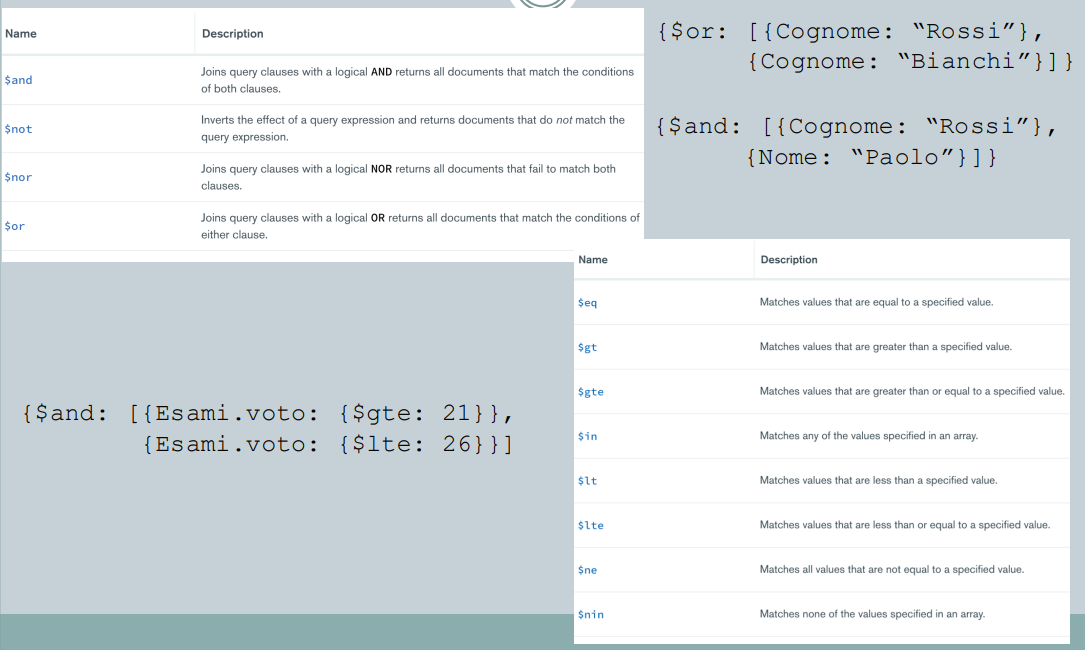
\includegraphics[width=1\linewidth]{image102}
	\caption{Operatori di Confronto}
	\label{fig:image102}
\end{figure}
\begin{figure}[H]
	\centering
	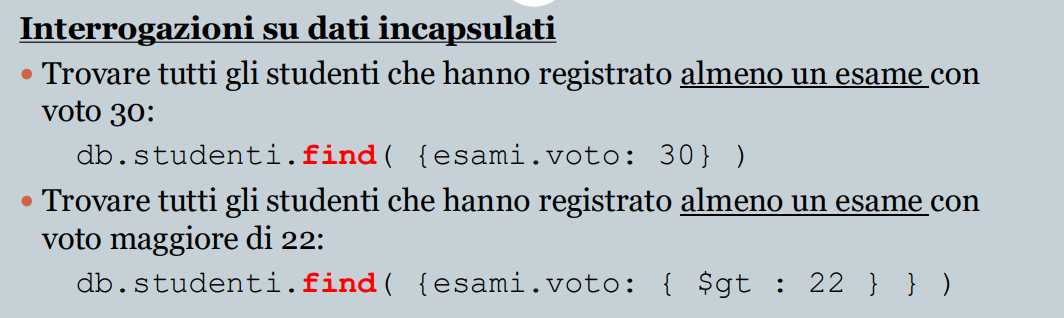
\includegraphics[width=1\linewidth]{image103}
	\caption{Esempio di interrogazioni con gli operatori}
	\label{fig:image103}
\end{figure}
\begin{figure}[H]
	\centering
	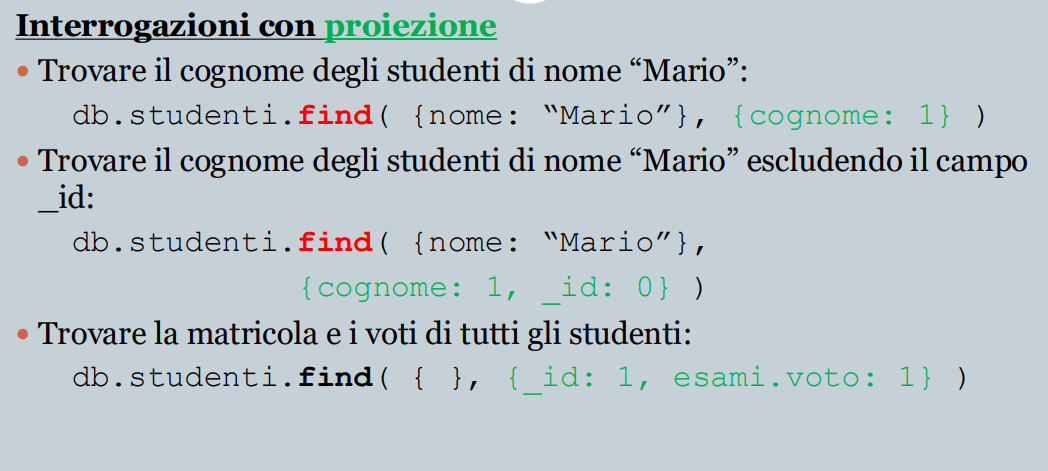
\includegraphics[width=1\linewidth]{image104}
	\caption{Interrogazioni con proiezione}
	\label{fig:image104}
\end{figure}
\begin{figure}[H]
	\centering
	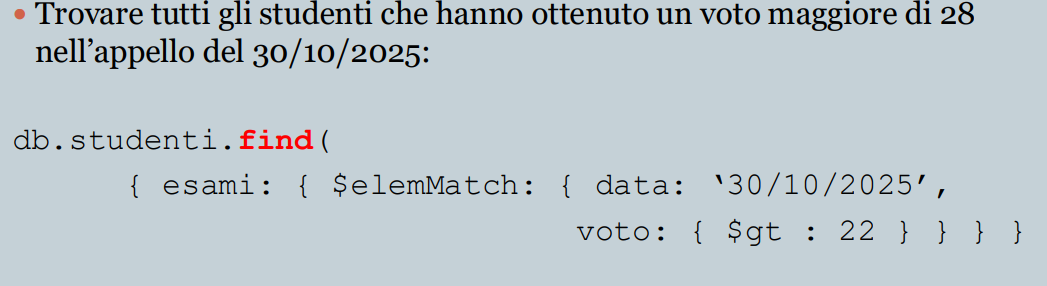
\includegraphics[width=1\linewidth]{image105}
	\caption{condizioni multiple}
	\label{fig:image105}
\end{figure}

	\section{Tecnologie - Transazioni}
\subsection{Tecnologia dei DBMS}
Un \textbf{DBMS} (Database Management System), o \textit{sistema di gestione di basi di dati}, 
è un sistema software progettato per gestire collezioni di dati che siano:

\begin{itemize}
	\item \textbf{Grandi} (di dimensioni tali da richiedere gestione su memoria secondaria);
	\item \textbf{Condivise} (accessibili da più utenti o applicazioni contemporaneamente);
	\item \textbf{Persistenti} (i dati sopravvivono all'esecuzione dei programmi che li utilizzano).
\end{itemize}

Un DBMS garantisce:
\begin{itemize}
	\item \textbf{Affidabilità} (integrità e recupero dei dati in caso di guasti);
	\item \textbf{Privatezza e sicurezza} (controllo degli accessi e gestione dei permessi).
\end{itemize}

Essendo un sistema software, un DBMS deve essere:
\begin{itemize}
	\item \textbf{Efficiente}, ottimizzando l’uso delle risorse (tempo di risposta e spazio);
	\item \textbf{Efficace}, fornendo strumenti adeguati per la gestione e l’organizzazione dei dati.
\end{itemize}

Le prestazioni e la qualità complessiva del sistema dipendono in modo significativo 
dalla \textbf{corretta progettazione della base di dati}.

Un DBMS:
\begin{itemize}
	\item Estende le funzionalità del \textit{file system};
	\item Gestisce collezioni di dati memorizzate in \textbf{memoria secondaria};
	\item Fornisce meccanismi di accesso, manipolazione e controllo dei dati.
\end{itemize}

\textbf{Base di dati:} una collezione organizzata di dati, gestita e controllata da un DBMS.
\subsection{Architettura su 3 livelli dei DBMS}
\begin{figure}[H]
	\centering
	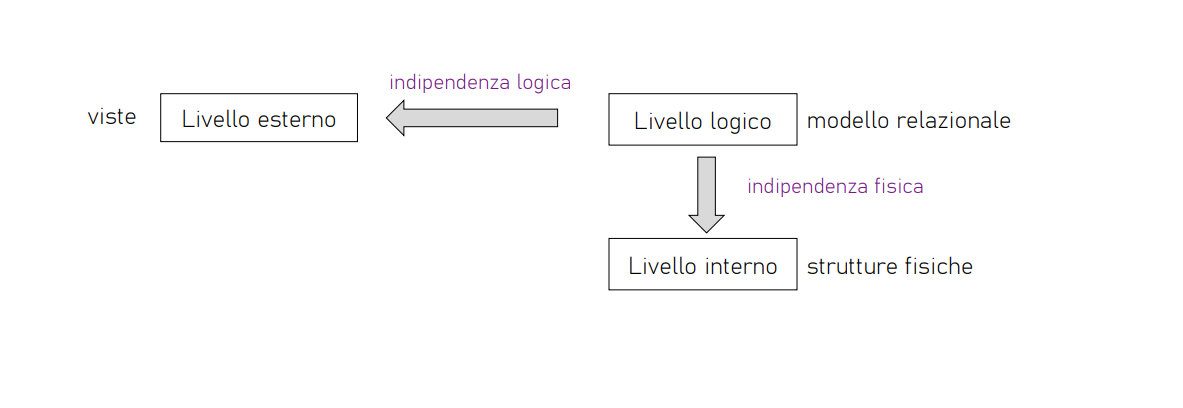
\includegraphics[width=1\linewidth]{image106}
	\caption{Architettura su 3 livelli dei DBMS}
	\label{fig:image106}
\end{figure}

Un DBMS è organizzato secondo un'architettura a tre livelli: \textbf{esterno}, \textbf{logico} e \textbf{interno}. 
Il \textbf{livello esterno} descrive le viste degli utenti: ad esempio, uno studente può visualizzare solo i propri voti, mentre la segreteria può accedere ai dati di tutti gli studenti. 
Il \textbf{livello logico} definisce la struttura concettuale della base di dati nel modello relazionale, ad esempio la tabella \texttt{Studenti(Matricola, Nome, Cognome, Corso)}, indipendentemente dalla memorizzazione fisica. 
Il \textbf{livello interno}, infine, descrive come i dati sono effettivamente memorizzati su disco, ad esempio in file organizzati in pagine con eventuali indici per ottimizzare le ricerche.

Questa separazione garantisce l'\textbf{indipendenza logica}, per cui modifiche allo schema logico non richiedono cambiamenti nelle viste esterne, e l'\textbf{indipendenza fisica}, per cui variazioni nell'organizzazione fisica dei dati non alterano lo schema logico.
\subsection{Transazione}
Una \textbf{transazione} è un'unità logica di lavoro eseguita da un programma applicativo che interagisce con una base di dati. 
È costituita da una sequenza di operazioni che devono essere considerate come un unico blocco indivisibile.

Una transazione deve garantire proprietà di \textbf{correttezza}, \textbf{robustezza} e \textbf{isolamento}, in modo da mantenere la consistenza della base di dati anche in presenza di errori o accessi concorrenti.

La caratteristica fondamentale di una transazione è il principio \textit{all-or-nothing}: 
essa o termina con successo (\textbf{commit}) producendo effetti permanenti sulla base di dati, oppure viene annullata (\textbf{abort/rollback}) senza lasciare alcuna modifica. 
\begin{figure}[H]
	\centering
	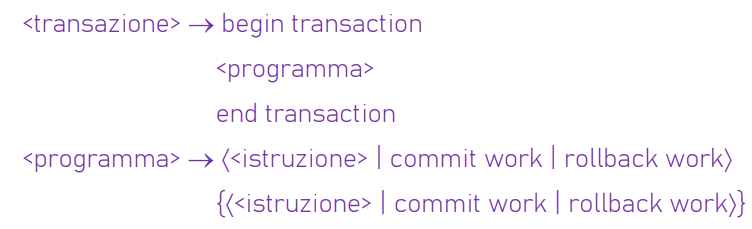
\includegraphics[width=1\linewidth]{image107}
	\caption{Sintassi di una transazione}
	\label{fig:image107}
\end{figure}
Una \textbf{transazione} si dice \emph{ben formata} se rispetta le seguenti condizioni:

\begin{itemize}
	\item Inizia esplicitamente con un'istruzione \texttt{BEGIN TRANSACTION}.
	
	\item Termina con un'istruzione \texttt{END TRANSACTION}.
	
	\item Durante la sua esecuzione viene raggiunto un punto di terminazione esplicito, 
	ovvero un'istruzione \texttt{COMMIT WORK} oppure \texttt{ROLLBACK WORK}.
	
	\item Dopo l'esecuzione di \texttt{COMMIT} o \texttt{ROLLBACK} non vengono effettuati 
	ulteriori accessi o modifiche alla base di dati all'interno della stessa transazione.
\end{itemize}
\begin{figure}[H]
	\centering
	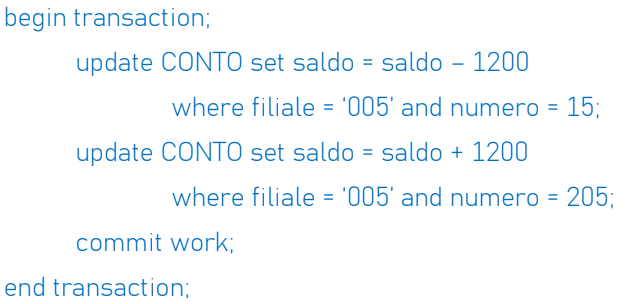
\includegraphics[width=1\linewidth]{image108}
	\caption{Esempio transazione ben formata}
	\label{fig:image108}
\end{figure}
\subsubsection{Proprietà delle transazioni}
Una transazione in un DBMS deve rispettare quattro proprietà fondamentali,
note come proprietà \textbf{ACID}:

\begin{itemize}
	
	\item \textbf{Atomicità (Atomicity)}: una transazione è un'unità di esecuzione indivisibile. 
	Essa viene eseguita completamente oppure non viene eseguita affatto.
	
	Implicazioni:
	\begin{itemize}
		\item Se una transazione viene interrotta prima del \texttt{commit}, il lavoro eseguito fino a quel momento deve essere annullato, ripristinando lo stato della base di dati precedente all'inizio della transazione.
		
		\item Se una transazione viene interrotta dopo l'esecuzione del \texttt{commit} (commit completato con successo), il sistema deve garantire che gli effetti della transazione siano permanentemente registrati nella base di dati.
	\end{itemize}
	
	\item \textbf{Consistenza (Consistency)}: l'esecuzione di una transazione non deve violare i vincoli di integrità della base di dati.
	
	Implicazioni:
	\begin{itemize}
		\item \textbf{Verifica immediata}: il controllo dei vincoli viene effettuato durante l'esecuzione della transazione. Se un vincolo viene violato, viene annullata solo l'ultima operazione eseguita e il sistema restituisce all'applicazione una segnalazione di errore. L'applicazione può quindi reagire alla violazione.
		
		\item \textbf{Verifica differita}: il controllo dei vincoli viene effettuato al momento del \texttt{commit}. Se un vincolo di integrità risulta violato, l'intera transazione viene abortita senza possibilità per l'applicazione di reagire alla violazione.
	\end{itemize}
	
	\item \textbf{Isolamento (Isolation)}: l'esecuzione di una transazione deve essere indipendente dalla contemporanea esecuzione di altre transazioni.
	
	Implicazioni:
	\begin{itemize}
		\item Il rollback di una transazione non deve causare rollback a catena di altre transazioni che si trovano in esecuzione contemporaneamente.
		
		\item Il sistema deve regolare l'esecuzione concorrente tramite meccanismi di controllo dell'accesso alle risorse.
	\end{itemize}
	
	\item \textbf{Persistenza (Durability)}: l'effetto di una transazione che ha eseguito il \texttt{commit} non deve andare perso.
	
	Implicazioni:
	\begin{itemize}
		\item Il sistema deve essere in grado, in caso di guasto, di garantire gli effetti delle transazioni che al momento del guasto avevano già eseguito un \texttt{commit}.
	\end{itemize}
	
\end{itemize}
\subsection{Architettura di un DBMS}
Un DBMS è composto da diversi moduli che gestiscono le varie funzionalità
necessarie all'esecuzione delle transazioni.
\begin{figure}[H]
	\centering
	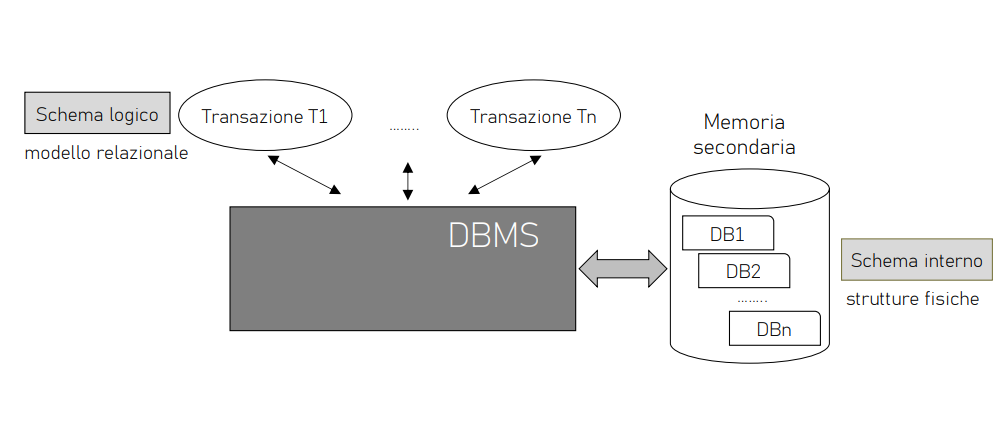
\includegraphics[width=1\linewidth]{image109}
	\caption{Architettura di riferimento di un DBMS}
	\label{fig:image109}
\end{figure}
La figura rappresenta l'interazione tra le transazioni degli utenti, il DBMS e la
memoria secondaria. Le transazioni (T1, \ldots, Tn) operano sullo \textbf{schema
	logico} del database secondo il modello relazionale e inviano le loro operazioni
al DBMS. Il \textbf{DBMS} funge da intermediario, gestendo l'esecuzione delle
transazioni e garantendo le proprietà di correttezza del sistema. I dati sono
memorizzati nella \textbf{memoria secondaria} (DB1, DB2, \ldots, DBn) secondo lo
\textbf{schema interno}, che descrive le strutture fisiche utilizzate per
organizzare e memorizzare i dati.
\begin{figure}[H]
	\centering
	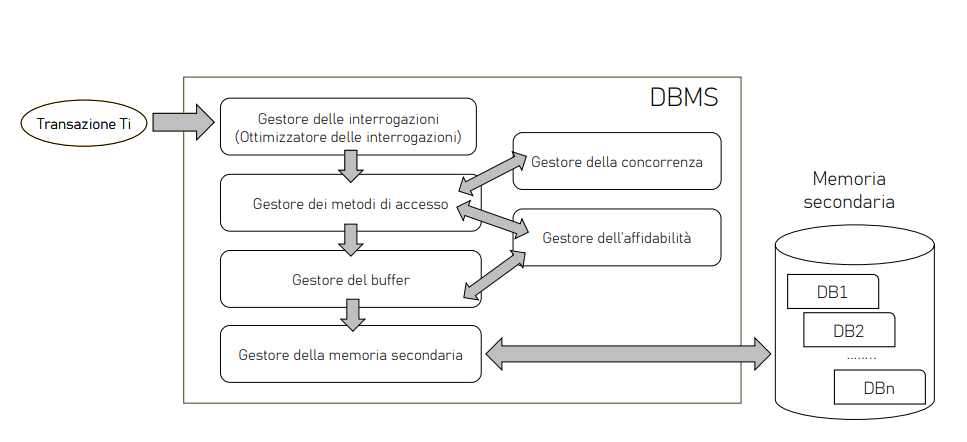
\includegraphics[width=1\linewidth]{image110}
	\caption{Moduli principali di un DBMS}
	\label{fig:image110}
\end{figure}
La figura mostra i principali moduli che compongono l'architettura interna di un
DBMS e il modo in cui collaborano durante l'esecuzione di una transazione.

Una transazione $T_i$ invia le proprie interrogazioni al \textbf{gestore delle
	interrogazioni} (query processor), che analizza e ottimizza le query per
determinare il piano di esecuzione più efficiente. Il \textbf{gestore dei metodi
	di accesso} stabilisce come accedere ai dati, utilizzando strutture come indici
o scansioni delle tabelle.

Il \textbf{gestore del buffer} si occupa della gestione delle pagine di dati in
memoria principale, mentre il \textbf{gestore della memoria secondaria} gestisce
l'accesso fisico ai dati memorizzati su disco.

Il \textbf{gestore della concorrenza} controlla l'esecuzione simultanea di più
transazioni per evitare interferenze, mentre il \textbf{gestore
	dell'affidabilità} garantisce la correttezza delle operazioni anche in caso di
guasti, assicurando il mantenimento delle proprietà ACID.
\begin{figure}[H]
	\centering
	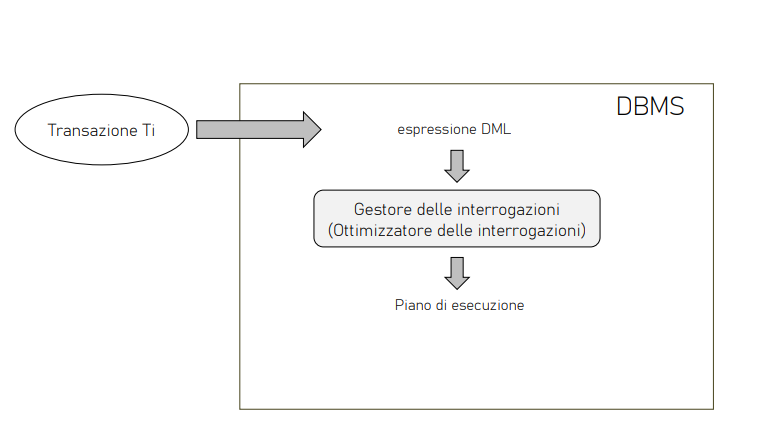
\includegraphics[width=1\linewidth]{image111}
	\caption{fase di elaborazione di una query}
	\label{fig:image111}
\end{figure}
Una transazione $T_i$ invia al DBMS un'espressione del linguaggio DML.
La query viene elaborata dal \textbf{gestore delle interrogazioni}
(query processor), che analizza e ottimizza l'interrogazione.
Il risultato di questo processo è un \textbf{piano di esecuzione},
ovvero una sequenza di operazioni che il DBMS esegue per ottenere
il risultato richiesto in modo efficiente.
\begin{figure}[H]
	\centering
	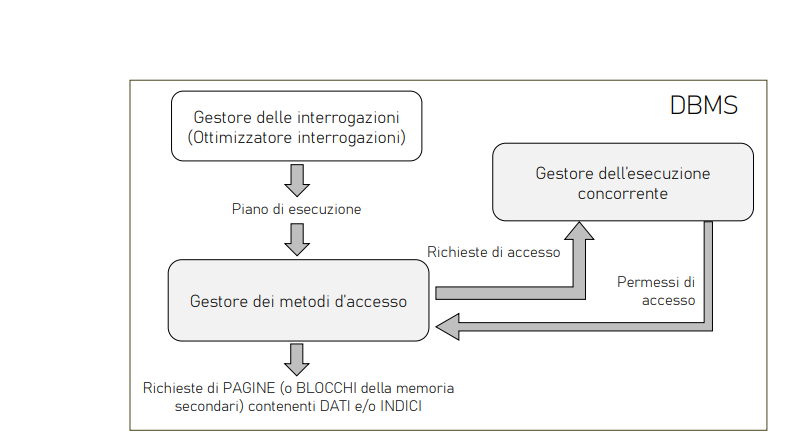
\includegraphics[width=1\linewidth]{image112}
	\caption{gestione delle interrogazioni}
	\label{fig:image112}
\end{figure}
Il piano di esecuzione prodotto dal gestore delle interrogazioni viene
eseguito dal gestore dei metodi di accesso, che richiede le pagine di
dati o indici dalla memoria secondaria. Le richieste di accesso ai dati
vengono controllate dal gestore dell'esecuzione concorrente, che verifica
la compatibilità con le altre transazioni in esecuzione e concede i
permessi di accesso. In questo modo il DBMS garantisce l'esecuzione
corretta delle transazioni concorrenti.
\begin{figure}[H]
	\centering
	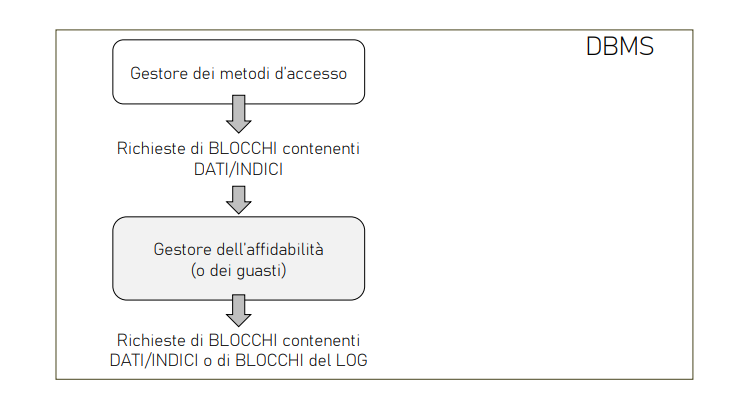
\includegraphics[width=1\linewidth]{image113}
	\caption{fase di recovery}
	\label{fig:image113}
\end{figure}
Le richieste di accesso ai blocchi contenenti dati o indici, generate dal
gestore dei metodi di accesso, vengono gestite dal \textbf{gestore
	dell'affidabilità} (recovery manager). Questo modulo ha il compito di
garantire la correttezza del database anche in caso di guasti,
utilizzando il \textbf{log delle transazioni}. Il log registra le
operazioni eseguite dalle transazioni e permette al sistema di
ripristinare lo stato corretto della base di dati attraverso operazioni
di \emph{redo} e \emph{undo}.
\begin{figure}[H]
	\centering
	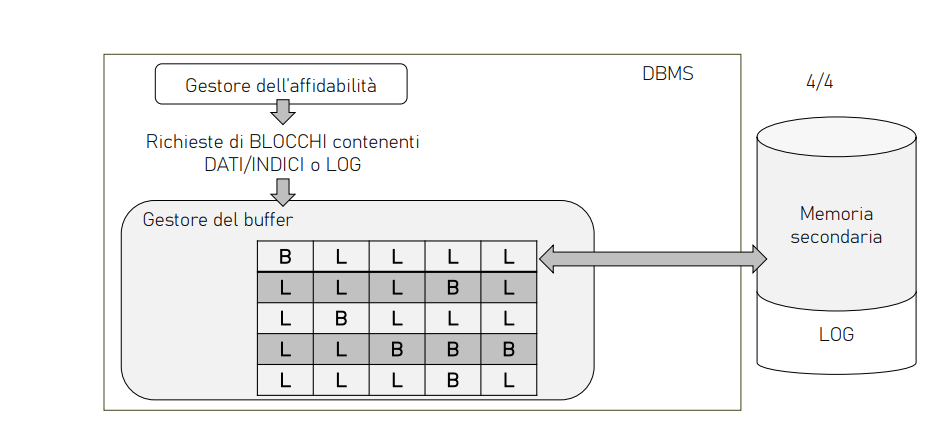
\includegraphics[width=1\linewidth]{image114}
	\caption{fase di gestione della memoria principale tramite il buffer manager quando accede ai dati sul disco}
	\label{fig:image114}
\end{figure}
Le richieste di accesso ai blocchi contenenti dati, indici o record del log,
generate dal gestore dell'affidabilità, vengono gestite dal
\textbf{gestore del buffer}. Questo modulo mantiene in memoria principale
una copia delle pagine utilizzate più frequentemente, riducendo gli
accessi alla memoria secondaria. Quando necessario, il buffer manager
carica nuove pagine dal disco o scrive sul disco le pagine modificate.
\begin{figure}[H]
	\centering
	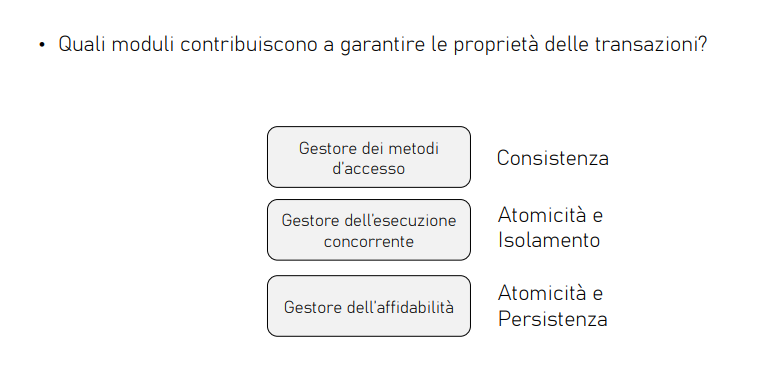
\includegraphics[width=1\linewidth]{image115}
	\caption{}
	\label{fig:image115}
\end{figure}

	\section{Strutture fisiche e accesso ai dati}

Per comprendere il funzionamento interno di un DBMS è necessario analizzare come i dati vengono effettivamente memorizzati e gestiti a livello fisico.

Una base di dati risiede in memoria secondaria per due motivi fondamentali. 
In primo luogo, per una questione di \textbf{dimensione}: le basi di dati sono generalmente molto grandi e non possono essere contenute interamente in memoria centrale. 
In secondo luogo, per garantire la \textbf{persistenza}: i dati devono sopravvivere all'esecuzione dei programmi e agli spegnimenti del sistema. 
A differenza della memoria centrale, che è volatile, la memoria secondaria consente di conservare le informazioni in modo permanente nel tempo.

La memoria secondaria presenta però alcune caratteristiche che influenzano direttamente il modo in cui i dati vengono gestiti. 
Essa non è direttamente accessibile dai programmi e i dati sono organizzati in \textbf{blocchi} (o pagine). 
Di conseguenza, non è possibile leggere una singola informazione in modo puntuale: quando si accede a un dato, è necessario caricare in memoria centrale l'intero blocco che lo contiene. 
Le uniche operazioni possibili sulla memoria secondaria sono quindi la \textbf{lettura} e la \textbf{scrittura} di blocchi.

Un aspetto cruciale è che tali operazioni hanno un costo molto elevato rispetto agli accessi alla memoria centrale, con una differenza di diversi ordini di grandezza. 
Per questo motivo, nella valutazione delle prestazioni di un DBMS non si considera il numero di operazioni di calcolo, ma il \textbf{numero di accessi alla memoria secondaria}, che rappresenta il vero collo di bottiglia del sistema.

Per ridurre il numero di accessi al disco interviene il \textbf{gestore del buffer} (buffer manager), che ha il compito di gestire la memoria centrale. 
Questo modulo mantiene in RAM i blocchi più utilizzati, evitando accessi ripetuti alla memoria secondaria. 
Quando un blocco non è presente in memoria, il buffer manager richiede il caricamento dal disco; analogamente, quando un blocco viene modificato, si occupa della sua scrittura in memoria secondaria.

Il \textbf{gestore della memoria secondaria} è invece responsabile dell'accesso fisico ai dati. 
Esso gestisce i file del database e si occupa delle operazioni di lettura e scrittura dei blocchi, interagendo direttamente con il file system del sistema operativo. 
In questo contesto, il gestore del buffer e quello della memoria secondaria collaborano strettamente: il primo richiede i blocchi necessari, mentre il secondo li recupera dal disco.

Infine, il \textbf{gestore dell'affidabilità} interviene per garantire la correttezza del sistema anche in presenza di guasti. 
Questo modulo mantiene un log delle operazioni eseguite e consente il ripristino dello stato corretto del database tramite operazioni di \textit{redo} e \textit{undo}, assicurando la persistenza delle transazioni completate.
L'interazione tra memoria secondaria e memoria centrale avviene tramite il \textbf{gestore del buffer}, che si occupa di trasferire i dati dal disco alla RAM sotto forma di blocchi.

In particolare, il buffer manager carica uno o più blocchi dalla memoria secondaria in \textbf{pagine} della memoria centrale. 
Sebbene non vi sia una corrispondenza perfetta, si assume generalmente che una pagina in memoria centrale corrisponda a un blocco in memoria secondaria.

Il buffer rappresenta quindi un'area di memoria centrale condivisa tra più applicazioni, il cui obiettivo è ridurre il numero di accessi alla memoria secondaria.

Il gestore del buffer ha il compito di:
\begin{itemize}
	\item caricare i blocchi dalla memoria secondaria alla memoria centrale;
	\item restituire riferimenti (puntatori) ai dati richiesti;
	\item scrivere i blocchi modificati dalla memoria centrale al disco.
\end{itemize}

Per ottimizzare le prestazioni, il buffer manager adotta diverse \textbf{politiche di gestione della memoria}, che riguardano sia le operazioni di lettura sia quelle di scrittura.

Nel caso della \textbf{lettura di un blocco}, si distinguono due situazioni:
\begin{itemize}
	\item se il blocco è già presente nel buffer (\textit{buffer hit}), non viene effettuato alcun accesso alla memoria secondaria e viene restituito direttamente il riferimento alla pagina in memoria centrale;
	\item se il blocco non è presente (\textit{buffer miss}), esso viene caricato dal disco e successivamente reso disponibile.
\end{itemize}

Nel caso della \textbf{scrittura}, il DBMS può adottare una strategia di \textbf{scrittura differita} (\textit{delayed write}): il blocco modificato viene aggiornato inizialmente solo in memoria centrale e la scrittura su disco viene posticipata. 
Questa scelta migliora le prestazioni riducendo il numero di operazioni di I/O, ma introduce il rischio di perdita dei dati in caso di guasto. 
Per questo motivo interviene il \textbf{gestore dell'affidabilità}, che tramite il log consente di ripristinare le informazioni corrette.

Le politiche di gestione del buffer si basano sul \textbf{principio di località}, secondo cui i dati recentemente utilizzati hanno un'alta probabilità di essere riutilizzati nel breve periodo.

Un'importante osservazione empirica è la cosiddetta \textbf{regola dell'80/20}: circa il 20\% dei dati è responsabile dell'80\% degli accessi. 
Questo implica che, mantenendo in memoria centrale una piccola parte dei dati più frequentemente utilizzati, è possibile ottenere un notevole miglioramento delle prestazioni.

Per questo motivo, politiche semplici come la LIFO (Last In First Out) risultano inefficaci, poiché non tengono conto del principio di località. 
Al contrario, strategie più evolute (come LRU, Least Recently Used) privilegiano il mantenimento in memoria dei dati utilizzati più di recente.
\subsection{Rappresentazione logica del buffer}

Il contenuto del buffer può essere rappresentato in maniera logica come una \textbf{matrice di pagine}, tutte aventi la stessa dimensione.

Ogni pagina del buffer può contenere un blocco $B$ proveniente dalla memoria secondaria. 
Si assume quindi, in prima approssimazione, una corrispondenza tra pagine in memoria centrale e blocchi in memoria secondaria.

Per ogni pagina del buffer che contiene un blocco, vengono mantenute due importanti \textbf{variabili di stato}:

\begin{itemize}
	\item un \textbf{contatore} $i$, che indica quante transazioni stanno attualmente utilizzando quella pagina;
	
	\item un \textbf{bit di stato} $j$ (dirty bit), che indica se la pagina è stata modificata:
	\begin{itemize}
		\item $j = 1$ se la pagina è stata modificata rispetto al contenuto in memoria secondaria;
		\item $j = 0$ se la pagina è identica a quella presente su disco.
	\end{itemize}
\end{itemize}

Il contatore $i$ è fondamentale per la gestione della concorrenza, in quanto impedisce la rimozione di una pagina ancora in uso da parte di una o più transazioni.

Il bit di stato $j$ è invece essenziale per la gestione delle scritture: una pagina modificata deve essere salvata su memoria secondaria prima di essere eventualmente rimossa dal buffer.

In Figura~\ref{fig:image188} è mostrata una possibile rappresentazione del buffer come matrice di pagine, in cui alcune pagine contengono blocchi della memoria secondaria e sono associate ai rispettivi stati.

\begin{figure}[H]
	\centering
	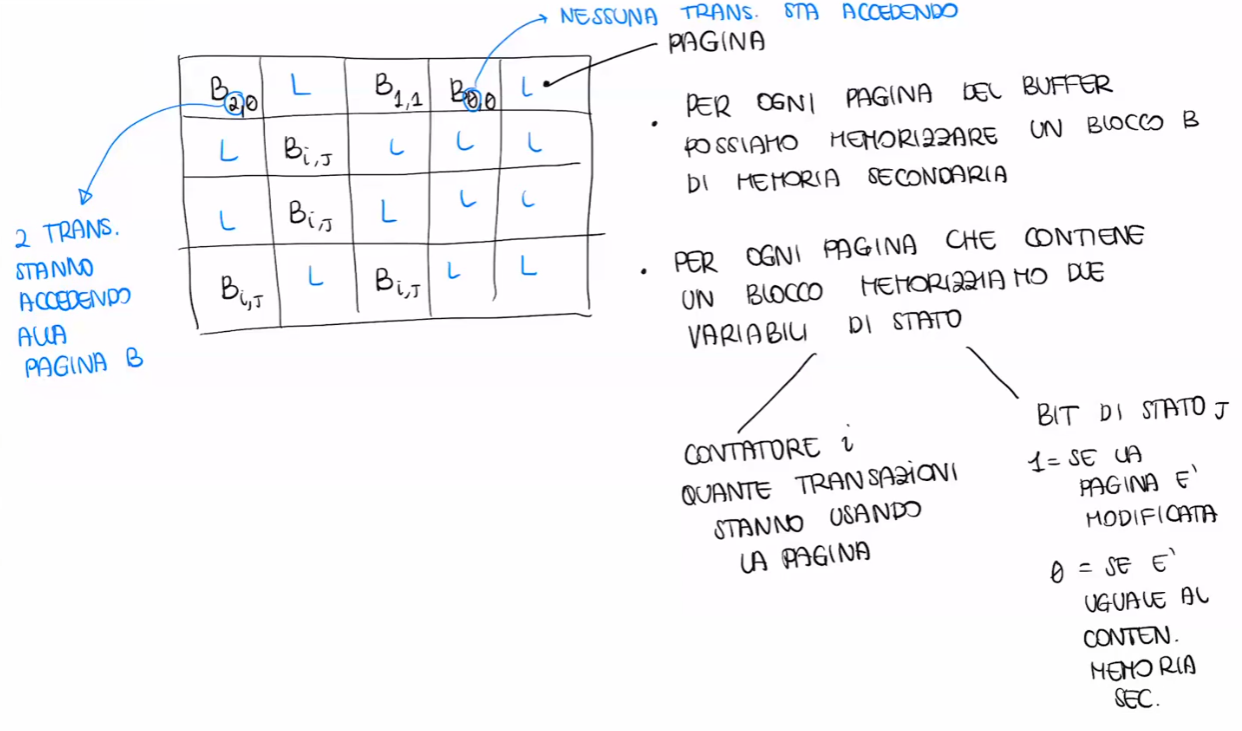
\includegraphics[width=1\linewidth]{image188}
	\caption{Rappresentazione logica del buffer}
	\label{fig:image188}
\end{figure}
\subsection{Primitive del gestore del buffer}

Il gestore del buffer mette a disposizione un insieme di primitive utilizzate principalmente dal gestore dei metodi di accesso per richiedere e gestire i blocchi in memoria centrale.

\begin{enumerate}
	\item \textbf{FIX}
	
	La primitiva FIX viene utilizzata per richiedere l'accesso a un blocco della memoria secondaria. 
	Essa restituisce un puntatore alla pagina del buffer che contiene il blocco richiesto.
	
	Il comportamento può essere descritto nei seguenti casi:
	
	\begin{itemize}
		\item \textbf{Caso 1: blocco già presente nel buffer (buffer hit)} \\
		Se il blocco è già caricato, il sistema restituisce semplicemente il puntatore alla pagina corrispondente.
		
		\item \textbf{Caso 2: blocco non presente (buffer miss)} \\
		Il sistema deve caricare il blocco in una pagina del buffer.
		
		\begin{itemize}
			\item Se esiste una \textbf{pagina libera} (indicata, ad esempio, con etichetta $L$ oppure con contatore $i = 0$), essa viene utilizzata.
			
			\item Se non esistono pagine libere, è necessario scegliere una pagina da sostituire secondo una politica di rimpiazzamento, come:
			\begin{itemize}
				\item \textbf{LRU} (Least Recently Used): rimuove la pagina meno recentemente utilizzata;
				\item \textbf{FIFO} (First In First Out): rimuove la pagina caricata da più tempo.
			\end{itemize}
		\end{itemize}
		
		Prima di riutilizzare una pagina, si verifica il valore del \textbf{dirty bit} $j$:
		\begin{itemize}
			\item se $j = 1$, la pagina deve essere scritta su disco tramite la primitiva \textit{FLUSH};
			\item se $j = 0$, può essere riutilizzata immediatamente.
		\end{itemize}
		
		\item \textbf{Caso 3: Gestione in assenza di pagine disponibili} \\
		Se tutte le pagine sono in uso (cioè con contatore $i > 0$), il DBMS può adottare due strategie:
		
		\begin{itemize}
			\item \textbf{NO-STEAL}: la transazione viene sospesa finché non si libera una pagina;
			\item \textbf{STEAL}: il sistema può sottrarre una pagina a un'altra transazione, anche se ancora in uso.
		\end{itemize}
	\end{itemize}
	
	Dopo il caricamento del blocco, il contatore $i$ della pagina viene incrementato.
	
	\item \textbf{UNFIX}
	
	La primitiva UNFIX indica che una transazione ha terminato di utilizzare un blocco. 
	Di conseguenza, il contatore $i$ associato alla pagina viene decrementato.
	
	\item \textbf{SETDIRTY}
	
	Questa primitiva viene utilizzata quando una transazione modifica il contenuto di una pagina. 
	Il dirty bit $j$ viene posto a 1, indicando che la copia in memoria centrale è diversa da quella in memoria secondaria.
	
	\item \textbf{FLUSH}
	
	La primitiva FLUSH consente di scrivere su memoria secondaria una pagina modificata. 
	Questa operazione può avvenire in modo asincrono ed è utilizzata dal gestore del buffer per liberare spazio.
	
	Al termine dell'operazione, il dirty bit $j$ viene posto a 0.
	
	\item \textbf{FORCE}
	
	La primitiva FORCE è una variante della FLUSH, utilizzata per garantire la scrittura immediata di una pagina su memoria secondaria. 
	Essa è tipicamente richiesta dal gestore dell'affidabilità per assicurare la persistenza dei dati.
	
	Anche in questo caso, al termine dell'operazione il dirty bit $j$ viene posto a 0.
\end{enumerate}

	\section{Gestore metodi d'accesso}
Il \textbf{gestore dei metodi di accesso}, per operare correttamente, deve conoscere una serie di informazioni fondamentali:

\begin{itemize}
	\item l'\textbf{organizzazione delle tuple all'interno dei blocchi};
	\item come sono \textbf{organizzati i blocchi al loro interno}.
\end{itemize}

In particolare, è necessario comprendere come è strutturata una \textbf{pagina} (o blocco) in memoria secondaria.
\begin{figure}[H]
	\centering
	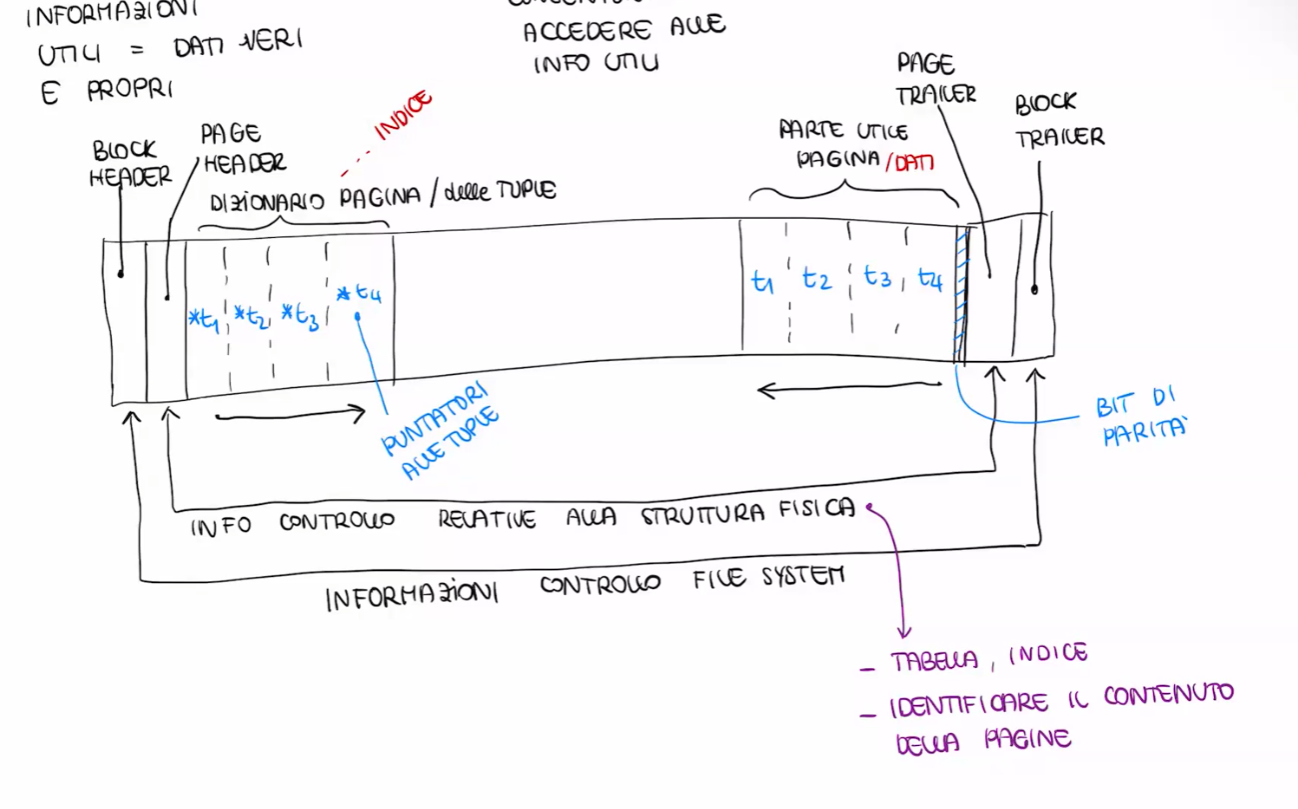
\includegraphics[width=1\linewidth]{image199}
	\caption{Struttura pagina}
	\label{fig:image199}
\end{figure}
Una pagina contiene due tipologie principali di informazioni:

\begin{itemize}
	\item \textbf{informazioni utili} (dati veri e propri), ovvero le tuple memorizzate;
	\item \textbf{informazioni di controllo}, che permettono di gestire e accedere correttamente ai dati.
\end{itemize}

Le informazioni di controllo sono fondamentali, poiché consentono al DBMS di localizzare, interpretare e manipolare i dati presenti nella pagina.

All'inizio e alla fine del blocco sono presenti strutture di controllo legate al file system:

\begin{itemize}
	\item \textbf{Block Header}: contiene informazioni di gestione del blocco;
	\item \textbf{Block Trailer}: contiene informazioni di controllo aggiuntive (ad esempio per verifiche di integrità).
\end{itemize}

Sono inoltre presenti informazioni di controllo relative alla \textbf{struttura fisica}, che permettono di:
\begin{itemize}
	\item identificare a quale tabella appartengono i dati;
	\item determinare se il blocco contiene dati o indici;
	\item interpretare correttamente il contenuto della pagina.
\end{itemize}

All'interno della pagina si distinguono due aree principali di memoria, che crescono in direzioni opposte:

\begin{itemize}
	\item il \textbf{dizionario della pagina} (o slot directory), che contiene puntatori alle tuple;
	\item la \textbf{parte utile della pagina}, che contiene effettivamente le tuple (dati).
\end{itemize}

Il dizionario della pagina può essere visto come una sorta di indice interno, che consente di accedere rapidamente alle tuple presenti nella pagina.

Un elemento importante è il \textbf{bit di parità}, utilizzato per verificare l'integrità dei dati e rilevare eventuali corruzioni delle informazioni.

Il dizionario delle tuple è necessario soprattutto quando le tuple hanno \textbf{lunghezza variabile}.

\begin{itemize}
	\item Nel caso di tuple a \textbf{lunghezza fissa}, non è necessario un dizionario, poiché la posizione delle tuple può essere calcolata direttamente.
	
	\item Tuttavia, questa soluzione è inefficiente, in quanto può causare \textbf{spreco di spazio}.
	
	\item Nel caso di tuple a \textbf{lunghezza variabile}, è invece necessario un dizionario, che memorizza per ogni tupla l'\textbf{offset di inizio} all'interno della pagina.
\end{itemize}

In questo modo, il DBMS può accedere direttamente alle tuple senza dover scansionare l'intero blocco, migliorando significativamente le prestazioni.
\subsection{Operazioni sulle pagine}

Il gestore dei metodi di accesso deve supportare diverse operazioni sulle pagine (blocchi), tra cui inserimento, cancellazione e accesso ai dati.

\subsubsection{Inserimento}

Nel caso di inserimento di una nuova tupla, si possono verificare tre situazioni:

\begin{itemize}
	\item \textbf{Spazio contiguo sufficiente} \\
	È il caso più semplice: la tupla viene inserita nella parte utile della pagina e il \textbf{dizionario della pagina} viene aggiornato con il nuovo puntatore (offset) alla tupla.
	
	\item \textbf{Spazio insufficiente} \\
	Se non esiste spazio sufficiente all'interno della pagina, è necessario interagire con il file system per allocare un \textbf{nuovo blocco}, nel quale verrà inserita la tupla.
	
	\item \textbf{Spazio sufficiente ma non contiguo} \\
	In questo caso è necessario effettuare una \textbf{riorganizzazione della pagina} (compattazione), in modo da rendere lo spazio libero contiguo. 
	Dopo la riorganizzazione, l'inserimento avviene come nel caso semplice.
\end{itemize}

\subsubsection{Cancellazione}

La cancellazione di una tupla è sempre possibile e generalmente non richiede una riorganizzazione immediata della pagina.

In particolare:
\begin{itemize}
	\item viene rimosso il riferimento alla tupla dal dizionario;
	\item lo spazio occupato dalla tupla viene marcato come libero.
\end{itemize}

Eventuali operazioni di compattazione possono essere eseguite in un secondo momento per ottimizzare lo spazio.

\subsubsection{Accesso}

L'accesso ai dati può avvenire in due modalità principali:

\begin{itemize}
	\item \textbf{Accesso a una tupla} \\
	Se è noto l'offset della tupla, si utilizza il \textbf{dizionario della pagina} per accedere direttamente alla posizione corretta. 
	In caso di accesso a più tuple, può essere conveniente effettuare una \textbf{scansione sequenziale} della pagina.
	
	\item \textbf{Accesso a un attributo} \\
	Per accedere a un attributo specifico, è necessario prima individuare la tupla. 
	Una volta identificata, si accede all'attributo tramite un meccanismo basato sugli \textbf{offset} interni alla tupla, che permettono di localizzare i singoli campi.
\end{itemize}
\subsection{Criteri di organizzazione delle tuple nei blocchi}

Le tuple all'interno dei blocchi possono essere organizzate secondo diversi criteri, in base a come vogliamo accedere ai dati.

Le principali modalità sono:

\begin{itemize}
	\item \textbf{Organizzazione sequenziale}: le tuple sono memorizzate una dopo l'altra, tipicamente nell'ordine di inserimento.
	
	\item \textbf{Accesso calcolato (hash)}: la posizione delle tuple è determinata da una funzione di hash, che permette un accesso diretto.
	
	\item \textbf{Strutture ad albero}: i dati sono organizzati tramite indici (es. B+-tree), per rendere più efficienti le ricerche.
\end{itemize}

\subsection{Organizzazione sequenziale dei file}

Consideriamo ora il caso più semplice: l'\textbf{organizzazione sequenziale}.

I dati sono salvati in file composti da blocchi logicamente consecutivi.  
Possiamo avere due varianti:

\begin{itemize}
	\item \textbf{Sequenziale disordinata (seriale)} → le tuple sono nell'ordine di inserimento
	\item \textbf{Sequenziale ordinata} → le tuple sono ordinate secondo una chiave
\end{itemize}

\subsubsection{Sequenziale disordinata (seriale)}

È la struttura più semplice e più intuitiva.

\paragraph{Inserimento}
L'inserimento è molto veloce:
\begin{itemize}
	\item si prende l'ultimo blocco del file;
	\item si inserisce la tupla lì dentro (se c'è spazio);
	\item si fa in genere un solo accesso al disco.
\end{itemize}

\paragraph{Ricerca}
La ricerca è il punto debole:
\begin{itemize}
	\item bisogna scorrere tutti i blocchi;
	\item quindi serve una scansione sequenziale;
	\item nel caso peggiore: $N$ accessi alla memoria secondaria.
\end{itemize}

\paragraph{Cancellazione}
\begin{itemize}
	\item prima bisogna trovare la tupla;
	\item poi si elimina;
	\item non si compatta subito lo spazio.
\end{itemize}

\paragraph{Modifica}
\begin{itemize}
	\item si trova la tupla;
	\item se cambia dimensione (tuple variabili), potrebbe non starci più;
	\item quindi si fa: cancellazione + inserimento.
\end{itemize}

\paragraph{Problema principale}

Queste operazioni (soprattutto cancellazioni e modifiche) creano \textbf{frammentazione} e spreco di spazio.

Per questo motivo il DBMS può eseguire delle \textbf{riorganizzazioni periodiche}, che servono a:
\begin{itemize}
	\item compattare i dati;
	\item recuperare spazio;
	\item migliorare le prestazioni.
\end{itemize}
\subsubsection{Sequenziale ordinata}

La \textbf{struttura sequenziale ordinata} è un file sequenziale in cui le tuple sono memorizzate in ordine rispetto a una \textbf{chiave di ordinamento}.

In generale, questa chiave può essere diversa dalla \textbf{chiave primaria} ed è scelta per ottimizzare determinate operazioni di accesso.

\paragraph{Caratteristiche principali}

\begin{itemize}
	\item le tuple sono mantenute \textbf{ordinate} secondo la chiave;
	\item i blocchi sono logicamente consecutivi;
	\item è possibile sfruttare l'ordinamento per rendere più efficienti le ricerche.
\end{itemize}
\begin{figure}[H]
	\centering
	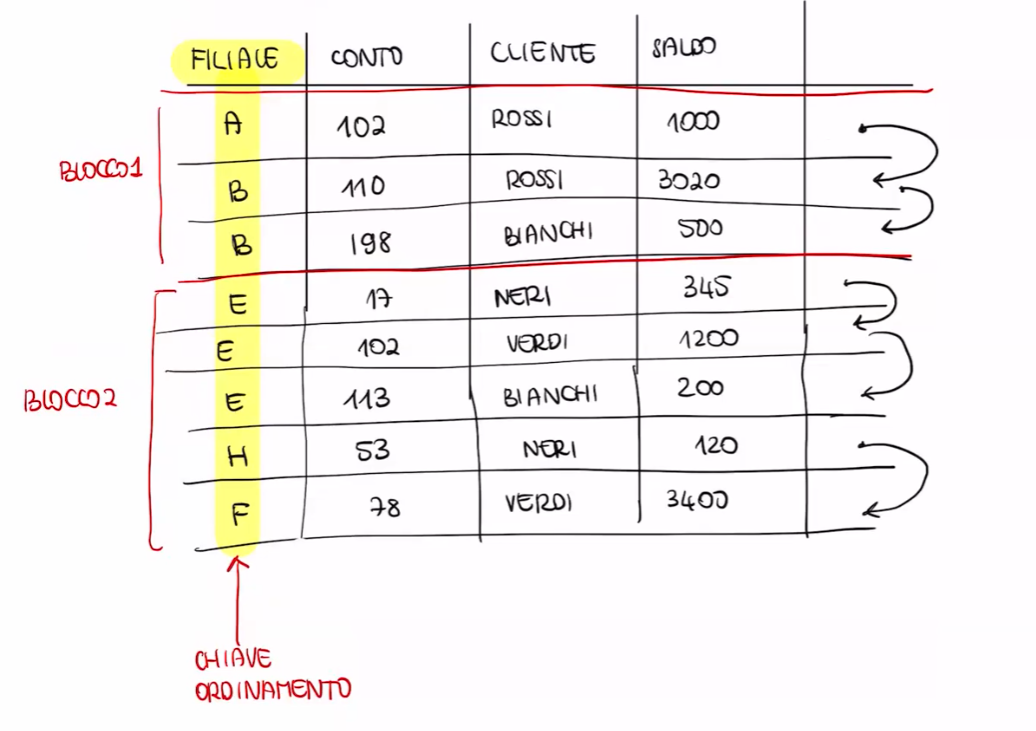
\includegraphics[width=0.75\linewidth]{image201}
	\caption{Esempio}
	\label{fig:image201}
\end{figure}
\begin{itemize}
	\item \textbf{Vantaggio} \\
	Rende efficienti tutte le operazioni che possono sfruttare l'\textbf{ordinamento}, 
	come ad esempio le ricerche per intervallo (es. ricerca per filiale).
	
	\item \textbf{Svantaggio} \\
	Le operazioni di aggiornamento (inserimento e modifica) devono mantenere l'ordinamento, 
	con un conseguente aumento del costo computazionale.
\end{itemize}
	\section{Gestione della concorrenza}

Una base di dati deve essere gestita da più programmi contemporaneamente, e si verifica quindi il problema della concorrenza. Per misurare il carico di lavoro si utilizza il \textbf{TPS} (\textit{Transaction Per Second}), un'unità di misura che quantifica le transazioni elaborate al secondo; per gestire il sistema con prestazioni accettabili, un valore tipico di TPS è compreso tra 100 e 1000.

La concorrenza può tuttavia produrre delle \textbf{anomalie}, note come problemi di concorrenza. Per gestire tali anomalie si introducono dei meccanismi di controllo delle esecuzioni concorrenti. Il componente del DBMS preposto a questo compito è il \textbf{gestore della concorrenza}, detto anche \textbf{scheduler}, il quale riceve le richieste di accesso ai dati e decide se autorizzarle o meno; quando non le autorizza immediatamente, decide di ritardarle.
\subsection{Anomalie da esecuzione concorrente}

Le principali anomalie che possono verificarsi durante l'esecuzione concorrente di transazioni sono le seguenti:

\begin{enumerate}
	\item \textbf{Perdita di aggiornamento} (\textit{lost update}): gli effetti di una transazione vengono sovrascritti e quindi persi da un'altra transazione eseguita concorrentemente.
	\item \textbf{Lettura inconsistente} (\textit{unrepeatable read}): accessi successivi alla stessa risorsa da parte della stessa transazione restituiscono risultati diversi.
	\item \textbf{Lettura sporca} (\textit{dirty read}): viene letto un dato che rappresenta uno stato intermedio di un'altra transazione, non ancora confermato.
	\item \textbf{Aggiornamento fantasma} (\textit{phantom update}): viene osservato uno stato intermedio che viola i vincoli di integrità.
	\item \textbf{Inserimento fantasma} (\textit{phantom insert}): valutazioni diverse di operazioni di aggregazione producono risultati diversi a causa di inserimenti concorrenti.
\end{enumerate}

L'obiettivo sarebbe evitarle tutte; tuttavia, vedremo che sarà necessario adottare un compromesso tra il grado di isolamento dalle anomalie e le prestazioni della base di dati.

Utilizzeremo la seguente notazione per gli esempi:
\begin{itemize}
	\item $t_i$ per indicare una transazione.
	\item $r_i(x)$ per indicare un'operazione di lettura effettuata dalla transazione $t_i$ sulla risorsa $x$.
	\item $w_i(x)$ per indicare un'operazione di scrittura effettuata dalla transazione $t_i$ sulla risorsa $x$.
\end{itemize}
\subsubsection{Perdita di aggiornamento}

Gli effetti di una transazione concorrente vengono sovrascritti e quindi persi. Consideriamo le seguenti transazioni:
\begin{align*}
	t_1 &: \text{BOT},\ r_1(x),\ x = x+1,\ w_1(x),\ \text{commit},\ \text{EOT} \\
	t_2 &: \text{BOT},\ r_2(x),\ x = x+1,\ w_2(x),\ \text{commit},\ \text{EOT}
\end{align*}

\begin{table}[H]
	\centering
	\begin{tabular}{|c|c|c|c|c|}
		\hline
		\textbf{Op. $t_1$} & \textbf{Seg. mem. centrale $t_1$} & \textbf{Memoria secondaria} & \textbf{Seg. mem. centrale $t_2$} & \textbf{Op. $t_2$} \\
		\hline
		\multicolumn{2}{|c|}{Stato iniziale} & $x = 2$ & \multicolumn{2}{c|}{Stato iniziale} \\
		\hline
		BOT & & 2 & & \\
		\hline
		$r_1(x)$ & 2 $\leftarrow$ & {[2]} & & \\
		\hline
		$x = x+1$ & 3 & {[2]} & & \\
		\hline
		& 3 & {[2]} & & BOT \\
		\hline
		& 3 & {[2]} $\rightarrow$ & 2 & $r_2(x)$ \\
		\hline
		& 3 & {[2]} & 3 & $x = x+1$ \\
		\hline
		& 3 & {[3]} $\leftarrow$ & 3 & $w_2(x)$ \\
		\hline
		$w_1(x)$ & 3 $\rightarrow$ & {[3]} & & EOT \\
		\hline
		commit & & {[3]} & & \\
		\hline
		EOT & & \cellcolor{green!30}{[3]} & & \\
		\hline
	\end{tabular}
	\caption{Esempio di perdita di aggiornamento: $t_2$ sovrascrive il valore scritto da $t_1$.}
\end{table}
Un'esecuzione seriale delle due transazioni avrebbe prodotto il risultato corretto $x = 4$; questa esecuzione concorrente ha invece prodotto $x = 3$, a causa della sovrascrittura dell'aggiornamento di $t_2$ da parte di $t_1$. Per evitare questo tipo di anomalia è necessario ricorrere a opportune tecniche di controllo della concorrenza.
\subsubsection{Lettura inconsistente}

Accessi successivi allo stesso dato all'interno della stessa transazione producono valori diversi. Consideriamo le seguenti transazioni:
\begin{align*}
	t_1 &: \text{BOT},\ r_1(x),\ r_1'(x),\ \text{commit},\ \text{EOT} \\
	t_2 &: \text{BOT},\ r_2(x),\ x = x+1,\ w_2(x),\ \text{commit},\ \text{EOT}
\end{align*}

Si noti che in $t_1$ le operazioni $r_1(x)$ e $r_1'(x)$ rappresentano due letture successive dello stesso dato $x$ all'interno della stessa transazione.

\begin{table}[H]
	\centering
	\begin{tabular}{|c|c|c|c|c|}
		\hline
		\textbf{Op. $t_1$} & \textbf{Seg. mem. centrale $t_1$} & \textbf{Memoria secondaria} & \textbf{Seg. mem. centrale $t_2$} & \textbf{Op. $t_2$} \\
		\hline
		\multicolumn{2}{|c|}{Stato iniziale} & $x = 2$ & \multicolumn{2}{c|}{Stato iniziale} \\
		\hline
		BOT & & 2 & & \\
		\hline
		$r_1(x)$ & 2 $\leftarrow$ & 2 & & \\
		\hline
		& 2 & 2 & & BOT \\
		\hline
		& 2 & 2 $\rightarrow$ & 2 & $r_2(x)$ \\
		\hline
		& 2 & 2 & 3 & $x = x+1$ \\
		\hline
		& 2 & 3 $\leftarrow$ & 3 & $w_2(x)$ \\
		\hline
		& 2 & 3 & 3 & commit \\
		\hline
		& 2 & 3 & 3 & EOT \\
		\hline
		\rowcolor{red!15}
		$r_1'(x)$ & 3 $\leftarrow$ & 3 & & \\
		\hline
		commit & & 3 & & \\
		\hline
		EOT & & 3 & & \\
		\hline
	\end{tabular}
	\caption{Esempio di lettura inconsistente: $t_1$ legge $x = 2$ la prima volta e $x = 3$ la seconda, pur non avendo mai modificato $x$.}
\end{table}

Si può notare che il valore letto da $t_1$ per $x$ è cambiato tra la prima e la seconda lettura, nonostante $t_1$ non abbia mai modificato $x$.
\subsubsection{Lettura sporca}

Viene letto un dato che rappresenta uno stato intermedio nell'evoluzione di una transazione. Consideriamo le seguenti transazioni:
\begin{align*}
	t_1 &: \text{BOT},\ r_1(x),\ \text{commit},\ \text{EOT} \\
	t_2 &: \text{BOT},\ r_2(x),\ x = x+1,\ w_2(x),\ \text{abort},\ \text{EOT}
\end{align*}

Poiché $t_2$ esegue un \textbf{abort}, la transazione viene annullata e i suoi effetti sulla base di dati vengono ripristinati (\textit{rollback}): è come se $t_2$ non fosse mai stata eseguita.

\begin{table}[H]
	\centering
	\begin{tabular}{|c|c|c|c|c|}
		\hline
		\textbf{Op. $t_1$} & \textbf{Mem. centr. $t_1$} & \textbf{Memoria secondaria} & \textbf{Mem. centr. $t_2$} & \textbf{Op. $t_2$} \\
		\hline
		\multicolumn{2}{|c|}{Stato iniziale} & $x = 2$ & \multicolumn{2}{c|}{Stato iniziale} \\
		\hline
		BOT & & 2 & & \\
		\hline
		& & 2 & & BOT \\
		\hline
		& & 2 $\rightarrow$ & 2 & $r_2(x)$ \\
		\hline
		& & 2 & 3 & $x = x+1$ \\
		\hline
		& & 3 $\leftarrow$ & 3 & $w_2(x)$ \\
		\hline
		\rowcolor{red!15}
		$r_1(x)$ & 3 $\leftarrow$ & 3 & & \\
		\hline
		\rowcolor{red!15}
		commit & \textcolor{red}{3} & \textcolor{red}{2} & & abort \\
		\hline
		EOT & & 2 & & EOT \\
		\hline
	\end{tabular}
	\caption{Esempio di lettura sporca: $t_1$ legge il valore $x = 3$ scritto da $t_2$, che però esegue abort e ripristina $x = 2$.}
\end{table}

Il valore 3 letto da $t_1$ non è conforme al contenuto reale della memoria secondaria: poiché $t_2$ ha eseguito l'abort, i suoi effetti sono stati annullati e il valore corretto di $x$ rimane 2. $t_1$ ha quindi letto uno stato intermedio che non avrebbe dovuto essere visibile.
\subsubsection{Aggiornamento fantasma}

Osservazione di uno stato intermedio che non soddisfa i vincoli di integrità. Supponiamo di avere tre risorse $x$, $y$, $z$ con il vincolo che la loro somma debba essere maggiore o uguale a 100:
\[
x + y + z \geq 100
\]

Consideriamo le seguenti transazioni:
\begin{align*}
	t_1 &: \text{BOT},\ r_1(y),\ r_1(x),\ r_1(z),\ S = x+y+z,\ \text{EOT} \\
	t_2 &: \text{BOT},\ r_2(y),\ y = y+10,\ r_2(z),\ z = z-10,\ w_2(y),\ w_2(z),\ \text{commit},\ \text{EOT}
\end{align*}

Si noti che $t_2$ non viola il vincolo: sposta semplicemente 10 unità da $z$ a $y$, lasciando invariata la somma. Tuttavia, a causa dell'interleaving, $t_1$ può osservare uno stato intermedio in cui il vincolo risulta violato.

\begin{table}[H]
	\centering
	\begin{tabular}{|c|c|c|c|c|}
		\hline
		\textbf{Op. $t_1$} & \textbf{Mem. centr. $t_1$} & \textbf{Memoria secondaria} & \textbf{Mem. centr. $t_2$} & \textbf{Op. $t_2$} \\
		\hline
		\multicolumn{2}{|c|}{Stato iniziale} & $(x,y,z) = 20, 20, 60$ & \multicolumn{2}{c|}{Stato iniziale} \\
		\hline
		BOT & & 20, 20, 60 & & \\
		\hline
		$r_1(y)$ & $-,20,-$ $\leftarrow$ & 20, 20, 60 & & \\
		\hline
		& $-,20,-$ & 20, 20, 60 & & BOT \\
		\hline
		& $-,20,-$ & 20, 20, 60 $\rightarrow$ & $-,20,-$ & $r_2(y)$ \\
		\hline
		& $-,20,-$ & 20, 20, 60 & $-,30,-$ & $y = y+10$ \\
		\hline
		& $-,20,-$ & 20, 20, 60 $\rightarrow$ & $-,30,60$ & $r_2(z)$ \\
		\hline
		& $-,20,-$ & 20, 20, 60 & $-,30,50$ & $z = z-10$ \\
		\hline
		& $-,20,-$ & 20, 30, 60 $\leftarrow$ & $-,30,50$ & $w_2(y)$ \\
		\hline
		& $-,20,-$ & \cellcolor{yellow!40}20, 30, 50 $\leftarrow$ & $-,30,50$ & $w_2(z)$ \\
		\hline
		& $-,20,-$ & \cellcolor{yellow!40}20, 30, 50 & & commit \textcolor{green!50!black}{(vincolo OK)} \\
		\hline
		\rowcolor{red!15}
		$r_1(x)$ & 20, 20, 50 & \cellcolor{yellow!40}20, 30, 50 & & \\
		\hline
		\rowcolor{red!15}
		$r_1(z)$ & 20, 20, 50 &  & & \textcolor{red}{vincolo violato per $t_1$!} \\
		\hline
	\end{tabular}
	\caption{Aggiornamento fantasma: $t_2$ non viola il vincolo, ma $t_1$ osserva uno stato intermedio in cui $x + y + z = 20 + 20 + 50 = 90 < 100$.}
\end{table}
\subsubsection{Inserimento fantasma}

Valutazioni diverse di operatori di aggregazione ($\text{SUM}$, $\text{COUNT}$, $\text{AVG}$, $\text{MAX}$, $\text{MIN}$) all'interno della stessa transazione producono risultati diversi. È un'anomalia simile alla lettura inconsistente, ma coinvolge operatori di aggregazione anziché singoli valori.

La differenza sostanziale rispetto alle anomalie precedenti risiede nella natura della risorsa coinvolta: non si tratta di un singolo dato, ma dell'intera tabella. L'anomalia si manifesta quando, tra due valutazioni successive dello stesso operatore di aggregazione, un'altra transazione inserisce nuove tuple, alterando il risultato.
\subsection{Schedule}

Uno \textbf{schedule} è una sequenza di operazioni di lettura e scrittura eseguite su risorse della base di dati da transazioni concorrenti. Date le seguenti transazioni:
\begin{align*}
	t_1 &: \text{BOT},\ r_1(x),\ w_1(x),\ \text{commit},\ \text{EOT} \\
	t_2 &: \text{BOT},\ r_2(x),\ w_2(x),\ \text{commit},\ \text{EOT}
\end{align*}

Un possibile schedule è ad esempio:
\[
S: r_1(x),\ r_2(x),\ w_2(x),\ w_1(x)
\]

Date due o più transazioni, esistono più schedule possibili. L'obiettivo è accettare solo gli schedule che evitano le anomalie, ovvero gli schedule equivalenti a uno schedule seriale.

Uno \textbf{schedule seriale} è uno schedule in cui le operazioni di ogni transazione compaiono in sequenza, senza essere inframmezzate da operazioni di altre transazioni. Ad esempio:
\begin{align*}
	S_1 &: r_1(x),\ r_2(x),\ w_2(x),\ w_1(x) \quad \text{(non seriale)} \\
	S_2 &: r_1(x),\ w_1(x),\ r_2(x),\ w_2(x) \quad \text{(seriale)} \\
	S_3 &: r_2(x),\ w_2(x),\ r_1(x),\ w_1(x) \quad \text{(seriale)}
\end{align*}

L'obiettivo del gestore della concorrenza è individuare gli schedule \textbf{serializzabili}, ovvero equivalenti a uno schedule seriale. Per equivalenza si intende che lo schedule produce lo stesso effetto sulla base di dati che si otterrebbe eseguendo le transazioni una di seguito all'altra. È quindi necessario definire formalmente quando uno schedule è equivalente a uno schedule seriale.
\subsubsection{Ipotesi di commit-proiezione}

Per semplificare l'analisi, supponiamo che l'esito di tutte le transazioni sia noto a priori. In base a questa ipotesi, escludiamo dagli schedule le operazioni delle transazioni che terminano con un abort, considerando quindi solo le transazioni che giungono a buon fine con un commit.

Introdurremo due nozioni di equivalenza tra schedule:
\begin{enumerate}
	\item \textbf{View equivalenza}
	\item \textbf{Conflict equivalenza}
\end{enumerate}
\subsubsection{View-Equivalenza}

La view equivalenza si basa su due relazioni fondamentali: \textit{legge-da} e \textit{scritture finali}.

\paragraph{Relazione legge-da.}
Dato uno schedule $S$, si dice che un'operazione di lettura $r_i(x)$ \textbf{legge-da} un'operazione di scrittura $w_j(x)$ se:
\begin{enumerate}
	\item $w_j(x)$ precede $r_i(x)$ in $S$;
	\item $j \neq i$;
	\item non esiste alcuna operazione $w_k(x)$ tra $w_j(x)$ e $r_i(x)$, ovvero $w_j(x)$ è la scrittura di $x$ immediatamente precedente a $r_i(x)$.
\end{enumerate}

Consideriamo i seguenti esempi:
\begin{align*}
	S_1 &: r_1(x),\ r_2(x),\ w_2(x),\ w_1(x) \quad \Rightarrow \quad \text{LEGGE\_DA}(S_1) = \emptyset \\
	& \text{\small($r_1(x)$ non è preceduta da alcuna scrittura; $r_2(x)$ è preceduta solo da $r_1(x)$, non da una scrittura)} \\[4pt]
	S_2 &: r_1(x),\ w_1(x),\ r_2(x),\ w_2(x) \quad \Rightarrow \quad \text{LEGGE\_DA}(S_2) = \{(r_2(x),\ w_1(x))\} \\
	& \text{\small($r_2(x)$ è preceduta da $w_1(x)$, che è la scrittura di $x$ immediatamente precedente)} \\[4pt]
	S_3 &: r_1(x),\ w_1(x),\ w_2(x),\ r_1(x) \quad \Rightarrow \quad \text{LEGGE\_DA}(S_3) = \emptyset \\
	& \text{\small(la seconda $r_1(x)$ è preceduta da $w_2(x)$, ma $i = 1 = k$, quindi la condizione $j \neq i$ non è soddisfatta)}
\end{align*}

\paragraph{Relazione scritture finali.}
Dato uno schedule $S$, un'operazione di scrittura $w_i(x)$ è una \textbf{scrittura finale} se è l'ultima operazione di scrittura su $x$ in $S$. Per ogni risorsa si individua quindi l'ultima transazione che ha effettuato una scrittura su di essa:
\[
S_1 : r_1(x),\ r_2(x),\ w_2(x),\ w_3(y),\ w_1(x) \quad \Rightarrow \quad \text{SCRITTURE\_FINALI}(S_1) = \{w_1(x),\ w_3(y)\}
\]

\paragraph{Definizione di view equivalenza.}
Due schedule $S_1$ e $S_2$ sono \textbf{view-equivalenti} ($S_1 \approx_V S_2$) se e solo se possiedono lo stesso insieme legge-da e lo stesso insieme di scritture finali.

Uno schedule $S$ è \textbf{view-serializzabile} se è view-equivalente a uno schedule seriale.
\paragraph{Esempio: perdita di aggiornamento.}

Consideriamo le transazioni:
\begin{align*}
	t_1 &: r_1(x),\ w_1(x) \\
	t_2 &: r_2(x),\ w_2(x)
\end{align*}

Uno schedule che rappresenta la perdita di aggiornamento è:
\[
S_{pa} : r_1(x),\ r_2(x),\ w_2(x),\ w_1(x)
\]

Calcoliamo le relazioni:
\begin{itemize}
	\item $\text{LEGGE\_DA}(S_{pa}) = \emptyset$: né $r_1(x)$ né $r_2(x)$ sono precedute da alcuna scrittura sullo stesso dato, quindi nessuna lettura legge-da una scrittura.
	\item $\text{SCRITTURE\_FINALI}(S_{pa}) = \{w_1(x)\}$: l'ultima operazione di scrittura su $x$ è $w_1(x)$, che compare per ultima tra le scritture.
\end{itemize}

Per determinare se $S_{pa}$ è view-serializzabile, dobbiamo verificare se esiste uno schedule seriale view-equivalente. Gli unici schedule seriali possibili sono:

\[
S_{12} : r_1(x),\ w_1(x),\ r_2(x),\ w_2(x)
\]
\begin{itemize}
	\item $\text{LEGGE\_DA}(S_{12}) = \{(r_2(x),\ w_1(x))\}$: $r_2(x)$ è preceduta immediatamente da $w_1(x)$.
	\item $\text{SCRITTURE\_FINALI}(S_{12}) = \{w_2(x)\}$: l'ultima scrittura su $x$ è $w_2(x)$.
\end{itemize}
$S_{12}$ non è view-equivalente a $S_{pa}$: differiscono sia nell'insieme legge-da che nelle scritture finali.

\[
S_{21} : r_2(x),\ w_2(x),\ r_1(x),\ w_1(x)
\]
\begin{itemize}
	\item $\text{LEGGE\_DA}(S_{21}) = \{(r_1(x),\ w_2(x))\}$: $r_1(x)$ è preceduta immediatamente da $w_2(x)$.
	\item $\text{SCRITTURE\_FINALI}(S_{21}) = \{w_1(x)\}$: l'ultima scrittura su $x$ è $w_1(x)$.
\end{itemize}
$S_{21}$ non è view-equivalente a $S_{pa}$: pur avendo le stesse scritture finali, l'insieme legge-da è diverso.

Poiché nessuno dei due schedule seriali è view-equivalente a $S_{pa}$, possiamo concludere che $\mathbf{S_{pa}}$ \textbf{non è view-serializzabile}.
\paragraph{Esempio: lettura inconsistente.}

Consideriamo le transazioni:
\begin{align*}
	t_1 &: r_1(x),\ r_1'(x) \\
	t_2 &: r_2(x),\ w_2(x)
\end{align*}

Lo schedule che rappresenta la lettura inconsistente è:
\[
S_{li} : r_1(x),\ r_2(x),\ w_2(x),\ r_1'(x)
\]

\begin{itemize}
	\item $\text{LEGGE\_DA}(S_{li}) = \{(r_1'(x),\ w_2(x))\}$: $r_1'(x)$ è preceduta immediatamente da $w_2(x)$, mentre $r_1(x)$ non è preceduta da alcuna scrittura.
	\item $\text{SCRITTURE\_FINALI}(S_{li}) = \{w_2(x)\}$: l'unica scrittura su $x$ è $w_2(x)$, che è quindi anche l'ultima.
\end{itemize}

Gli schedule seriali possibili sono:

\[
S_{12} : r_1(x),\ r_1'(x),\ r_2(x),\ w_2(x)
\]
\begin{itemize}
	\item $\text{LEGGE\_DA}(S_{12}) = \emptyset$: nessuna lettura è preceduta da una scrittura.
	\item $\text{SCRITTURE\_FINALI}(S_{12}) = \{w_2(x)\}$.
\end{itemize}
$S_{12}$ non è view-equivalente a $S_{li}$: l'insieme legge-da è diverso.

\[
S_{21} : r_2(x),\ w_2(x),\ r_1(x),\ r_1'(x)
\]
\begin{itemize}
	\item $\text{LEGGE\_DA}(S_{21}) = \{(r_1(x),\ w_2(x)),\ (r_1'(x),\ w_2(x))\}$: sia $r_1(x)$ che $r_1'(x)$ sono precedute immediatamente da $w_2(x)$.
	\item $\text{SCRITTURE\_FINALI}(S_{21}) = \{w_2(x)\}$.
\end{itemize}
$S_{21}$ non è view-equivalente a $S_{li}$: pur avendo le stesse scritture finali, l'insieme legge-da differisce — $S_{li}$ contiene solo $(r_1'(x),\ w_2(x))$, mentre $S_{21}$ contiene anche $(r_1(x),\ w_2(x))$.

Poiché $S_{li}$ non è view-equivalente ad alcuno schedule seriale, concludiamo che $\mathbf{S_{li}}$ \textbf{non è view-serializzabile}.
\paragraph{Esempio: verifica di view-serializzabilità.}

Consideriamo lo schedule:
\[
S_1 : r_1(x),\ w_1(x),\ r_2(z),\ r_1(y),\ w_1(y),\ r_2(x),\ w_2(x),\ w_2(z)
\]

Le transazioni coinvolte sono:
\begin{align*}
	t_1 &: r_1(x),\ w_1(x),\ r_1(y),\ w_1(y) \\
	t_2 &: r_2(z),\ r_2(x),\ w_2(x),\ w_2(z)
\end{align*}

Calcoliamo le relazioni per $S_1$:
\begin{itemize}
	\item $\text{LEGGE\_DA}(S_1) = \{(r_2(x),\ w_1(x))\}$: $r_2(x)$ è preceduta immediatamente da $w_1(x)$; $r_1(y)$, $r_2(z)$ e $r_1(x)$ non sono precedute da alcuna scrittura.
	\item $\text{SCRITTURE\_FINALI}(S_1) = \{w_2(x),\ w_1(y),\ w_2(z)\}$: $w_2(x)$ è l'ultima scrittura su $x$, $w_1(y)$ l'unica su $y$, $w_2(z)$ l'unica su $z$.
\end{itemize}

Gli schedule seriali possibili sono $S_{12}$ (prima $t_1$, poi $t_2$) e $S_{21}$ (prima $t_2$, poi $t_1$). Possiamo escludere immediatamente $S_{21}$: in $S_1$ la relazione legge-da impone $t_1 < t_2$ (poiché $r_2(x)$ legge-da $w_1(x)$), e le scritture finali impongono anch'esse $t_1 < t_2$ su $w_2(x)$; in $S_{21}$ l'ordine sarebbe invertito, quindi non può essere view-equivalente.

Verifichiamo $S_{12}$:
\[
S_{12} : r_1(x),\ w_1(x),\ r_1(y),\ w_1(y),\ r_2(z),\ r_2(x),\ w_2(x),\ w_2(z)
\]
\begin{itemize}
	\item $\text{LEGGE\_DA}(S_{12}) = \{(r_2(x),\ w_1(x))\}$
	\item $\text{SCRITTURE\_FINALI}(S_{12}) = \{w_2(x),\ w_1(y),\ w_2(z)\}$
\end{itemize}

Poiché $\text{LEGGE\_DA}(S_1) = \text{LEGGE\_DA}(S_{12})$ e $\text{SCRITTURE\_FINALI}(S_1) = \text{SCRITTURE\_FINALI}(S_{12})$, concludiamo che $S_1 \approx_V S_{12}$, quindi $\mathbf{S_1}$ \textbf{è view-serializzabile}.
\paragraph{Esempio: schedule non view-serializzabile.}

Consideriamo lo schedule:
\[
S_2 : r_1(x),\ w_1(x),\ w_3(x),\ r_2(y),\ r_3(y),\ w_3(y),\ w_1(y),\ r_2(x)
\]

Le transazioni coinvolte sono:
\begin{align*}
	t_1 &: r_1(x),\ w_1(x),\ w_1(y) \\
	t_2 &: r_2(y),\ r_2(x) \\
	t_3 &: w_3(x),\ r_3(y),\ w_3(y)
\end{align*}

Calcoliamo le relazioni per $S_2$:
\begin{itemize}
	\item $\text{LEGGE\_DA}(S_2) = \{(r_2(x),\ w_3(x))\}$: $r_2(x)$ è preceduta immediatamente da $w_3(x)$.
	\item $\text{SCRITTURE\_FINALI}(S_2) = \{w_3(x),\ w_1(y)\}$: $w_3(x)$ è l'ultima scrittura su $x$, $w_1(y)$ è l'ultima scrittura su $y$.
\end{itemize}

In linea di principio occorrerebbe esaminare tutte le $6$ permutazioni seriali possibili. Tuttavia, l'insieme delle scritture finali ci permette di escluderle tutte a priori imponendo due vincoli sull'ordine delle transazioni:
\begin{itemize}
	\item $w_3(x) \in \text{SCRITTURE\_FINALI}$ impone $t_1 < t_3$, affinché $w_1(x)$ non sovrascriva $w_3(x)$;
	\item $w_1(y) \in \text{SCRITTURE\_FINALI}$ impone $t_3 < t_1$, affinché $w_3(y)$ non sovrascriva $w_1(y)$.
\end{itemize}

I due vincoli sono contraddittori: non può esistere uno schedule seriale che soddisfi contemporaneamente $t_1 < t_3$ e $t_3 < t_1$. Pertanto, nessuna delle sei permutazioni può essere view-equivalente a $S_2$, e concludiamo che $\mathbf{S_2}$ \textbf{non è view-serializzabile}.
\paragraph{Esempio: schedule con 5 transazioni.}

Consideriamo lo schedule:
\[
S_3 : r_1(x),\ r_2(x),\ w_2(x),\ r_3(x),\ r_4(z),\ w_1(x),\ w_3(y),\ w_3(x),\ w_1(y),\ w_5(x),\ w_1(z),\ w_5(y),\ r_5(z)
\]

Le transazioni coinvolte sono:
\begin{align*}
	t_1 &: r_1(x),\ w_1(x),\ w_1(y),\ w_1(z) \\
	t_2 &: r_2(x),\ w_2(x) \\
	t_3 &: r_3(x),\ w_3(y),\ w_3(x) \\
	t_4 &: r_4(z) \\
	t_5 &: w_5(x),\ w_5(y),\ r_5(z)
\end{align*}

Calcoliamo le relazioni per $S_3$:
\begin{itemize}
	\item $\text{LEGGE\_DA}(S_3) = \{(r_3(x),\ w_2(x)),\ (r_5(z),\ w_1(z))\}$
	\item $\text{SCRITTURE\_FINALI}(S_3) = \{w_5(x),\ w_5(y),\ w_1(z)\}$
\end{itemize}

Ricaviamo ora i vincoli sull'ordine delle transazioni in qualsiasi schedule seriale view-equivalente a $S_3$.

\textbf{Dalle scritture finali:}
\begin{itemize}
	\item $w_5(x) \in \text{SCRITTURE\_FINALI}$ impone $t_2 < t_5$,\ $t_1 < t_5$,\ $t_3 < t_5$;
	\item $w_5(y) \in \text{SCRITTURE\_FINALI}$ impone $t_3 < t_5$,\ $t_1 < t_5$;
	\item $w_1(z) \in \text{SCRITTURE\_FINALI}$ non aggiunge vincoli ulteriori.
\end{itemize}

\textbf{Dall'insieme legge-da:}
\begin{itemize}
	\item $(r_3(x),\ w_2(x)) \in \text{LEGGE\_DA}$ impone $t_2 < t_3$, affinché $r_3(x)$ legga da $w_2(x)$;
	\item $(r_5(z),\ w_1(z)) \in \text{LEGGE\_DA}$ impone $t_1 < t_5$.
\end{itemize}

\textbf{Dalla non appartenenza a legge-da:}
Poiché $r_2(x)$ precede fisicamente $w_1(x)$ in $S_3$ e $(r_2(x),\ w_1(x)) \notin \text{LEGGE\_DA}(S_3)$, in qualsiasi schedule seriale equivalente $t_2$ deve precedere $t_1$, affinché $r_2(x)$ non legga da $w_1(x)$:
\[
t_2 < t_1
\]

\textbf{Contraddizione:} i vincoli ricavati impongono simultaneamente $t_2 < t_3$, $t_2 < t_1$ e $t_1 < t_5$, ma dall'insieme legge-da avevamo già ricavato $t_2 < t_3$ con $t_1 < t_2$ implicato dalla struttura dello schedule — il che genera un ciclo $t_2 < t_1 < t_2$. Non esiste quindi alcuno schedule seriale che soddisfi tutti i vincoli contemporaneamente, e concludiamo che $\mathbf{S_3}$ \textbf{non è view-serializzabile}.
\subsection{Conflict equivalenza}

\paragraph{Conflitto.}
Dato uno schedule $S$, si dice che una coppia di operazioni $(a_i, a_j)$ rappresenta un \textbf{conflitto} se:
\begin{itemize}
	\item $i \neq j$, ovvero le operazioni appartengono a transazioni diverse;
	\item entrambe operano sulla stessa risorsa;
	\item almeno una delle due è un'operazione di scrittura;
	\item $a_i$ compare prima di $a_j$ in $S$.
\end{itemize}

\paragraph{Conflict equivalenza.}
Due schedule $S_1$ e $S_2$ sono \textbf{conflict-equivalenti} ($S_1 \approx_C S_2$) se e solo se possiedono lo stesso insieme di conflitti.
\paragraph{Conflict-serializzabilità.}

Uno schedule $S$ è \textbf{conflict-serializzabile} (CSR) se esiste uno schedule seriale $S_r$ tale che $S \approx_C S_r$. Il vantaggio rispetto alla view-serializzabilità è che l'algoritmo per il test della conflict-serializzabilità ha complessità \textbf{lineare}.

\paragraph{Algoritmo CSR.}

Dato uno schedule $S$, l'algoritmo procede come segue:
\begin{enumerate}
	\item Costruire l'insieme dei conflitti di $S$.
	\item Costruire il \textbf{grafo dei conflitti} $G(N, A)$, dove:
	\begin{itemize}
		\item $N$ è l'insieme dei nodi, uno per ciascuna transazione di $S$;
		\item $A$ contiene un arco $(t_i, t_j)$ se esiste un conflitto $(a_i, a_j) \in S$.
	\end{itemize}
	\item Se il grafo dei conflitti è \textbf{aciclico}, allora $S$ è conflict-serializzabile; altrimenti non lo è.
\end{enumerate}

\paragraph{Dimostrazione di correttezza.}

\textbf{($\Rightarrow$) Se $S$ è CSR allora il suo grafo è aciclico.}
Sia $S_r$ lo schedule seriale conflict-equivalente a $S$, con le transazioni ordinate $t_1, t_2, \ldots, t_n$. Poiché $S \approx_C S_r$, i due schedule hanno esattamente gli stessi conflitti nello stesso ordine. Nel grafo dei conflitti di $S_r$ possono quindi comparire solo archi $(t_i, t_j)$ con $i < j$: un ciclo richiederebbe un arco $(t_j, t_i)$ con $j > i$, che implicherebbe l'esistenza di un conflitto in ordine inverso — impossibile in uno schedule seriale. Poiché $S$ e $S_r$ hanno lo stesso grafo, anche il grafo di $S$ è aciclico.

\textbf{($\Leftarrow$) Se il grafo di $S$ è aciclico allora $S$ è CSR.}
Se il grafo è aciclico, esiste un \textbf{ordinamento topologico}, ovvero una numerazione dei nodi tale che il grafo contenga solo archi $(t_i, t_j)$ con $i < j$. Utilizzando questo ordinamento topologico possiamo definire un ordine delle transazioni che produce lo stesso grafo dei conflitti di $S$: otteniamo così uno schedule seriale $S_r$ conflict-equivalente a $S$, quindi $S$ è CSR.

\paragraph{Esempio CSR: perdita di aggiornamento.}

Consideriamo lo schedule $S_{pa}$ già visto in precedenza:
\[
S_{pa} : r_1(x),\ r_2(x),\ w_2(x),\ w_1(x)
\]

Costruiamo l'insieme dei conflitti:
\[
\text{CONFLITTI}(S_{pa}) = \{(r_1(x),\ w_2(x)),\ (r_2(x),\ w_1(x)),\ (w_2(x),\ w_1(x))\}
\]
\begin{itemize}
	\item $(r_1(x),\ w_2(x))$: $r_1$ e $w_2$ operano sulla stessa risorsa $x$, appartengono a transazioni diverse, e $w_2$ è una scrittura;
	\item $(r_2(x),\ w_1(x))$: analogo, con $w_1$ scrittura;
	\item $(w_2(x),\ w_1(x))$: entrambe scritture sulla stessa risorsa $x$, transazioni diverse.
\end{itemize}
\begin{figure}[H]
	\centering
	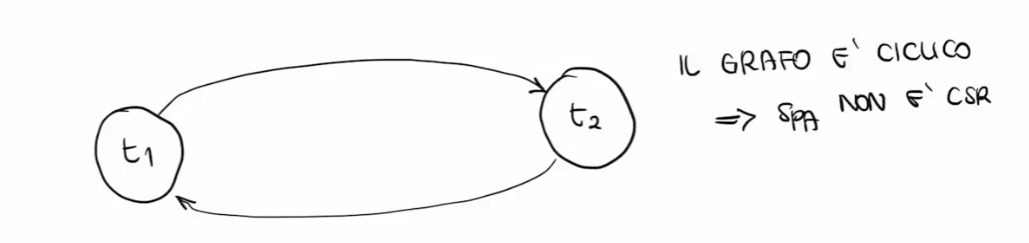
\includegraphics[width=0.7\linewidth]{image240}
	\label{fig:image240}
\end{figure}
Dal primo conflitto otteniamo un arco $t_1 \to t_2$; dal secondo e dal terzo un arco $t_2 \to t_1$. Il grafo dei conflitti contiene quindi un ciclo $t_1 \to t_2 \to t_1$, pertanto $\mathbf{S_{pa}}$ \textbf{non è CSR}.
\paragraph{Esempio CSR: lettura inconsistente.}

Consideriamo le transazioni:
\begin{align*}
	t_1 &: r_1(x),\ r_1'(x) \\
	t_2 &: r_2(x),\ w_2(x)
\end{align*}

Lo schedule è:
\[
S_{li} : r_1(x),\ r_2(x),\ w_2(x),\ r_1'(x)
\]

Costruiamo l'insieme dei conflitti:
\[
\text{CONFLITTI}(S_{li}) = \{(r_1(x),\ w_2(x)),\ (w_2(x),\ r_1'(x))\}
\]
\begin{itemize}
	\item $(r_1(x),\ w_2(x))$: $r_1$ precede $w_2$, stessa risorsa $x$, transazioni diverse, $w_2$ è scrittura $\Rightarrow$ arco $t_1 \to t_2$;
	\item $(w_2(x),\ r_1'(x))$: $w_2$ precede $r_1'$, stessa risorsa $x$, transazioni diverse, $w_2$ è scrittura $\Rightarrow$ arco $t_2 \to t_1$.
\end{itemize}
\begin{figure}[H]
	\centering
	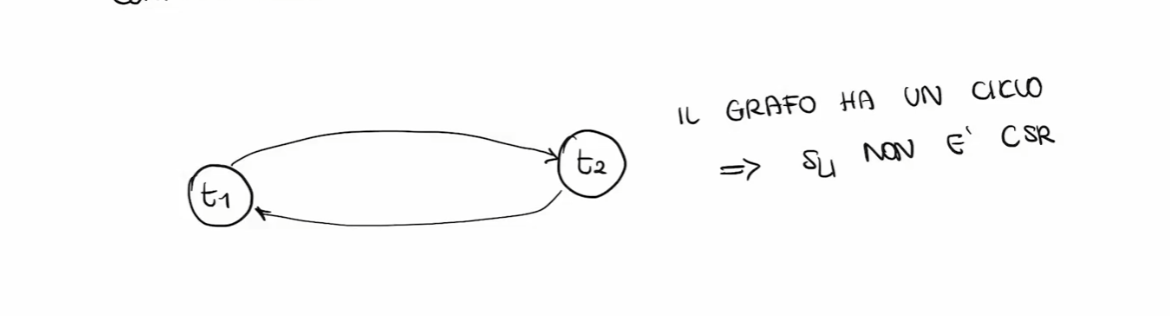
\includegraphics[width=1\linewidth]{image241}
	\label{fig:image241}
\end{figure}
Il grafo dei conflitti contiene un ciclo $t_1 \to t_2 \to t_1$, pertanto $\mathbf{S_{li}}$ \textbf{non è CSR}.
\subsection{Relazione tra CSR e VSR}

La conflict-serializzabilità è una condizione \textbf{sufficiente ma non necessaria} per la view-serializzabilità. In altri termini:

\begin{itemize}
	\item $S \in \text{CSR} \Rightarrow S \in \text{VSR}$: se uno schedule è conflict-serializzabile, allora è anche view-serializzabile.
	\item $S \notin \text{CSR} \not\Rightarrow S \notin \text{VSR}$: se uno schedule non è conflict-serializzabile, non possiamo concludere nulla sulla sua view-serializzabilità.
	\item $S \notin \text{VSR} \Rightarrow S \notin \text{CSR}$: se uno schedule non è view-serializzabile, allora non è nemmeno conflict-serializzabile.
\end{itemize}

Quindi l'insieme CSR è un sottoinsieme proprio di VSR: esistono schedule view-serializzabili che non sono conflict-serializzabili, ma non viceversa.

\paragraph{Strategia per gli esercizi.}
Data uno schedule $S$, la procedura da seguire è:
\begin{enumerate}
	\item Applicare il \textbf{test CSR}: costruire il grafo dei conflitti e verificare se è aciclico.
	\begin{itemize}
		\item Se $S$ è CSR $\Rightarrow$ $S$ è anche VSR. Non è necessario proseguire.
		\item Se $S$ non è CSR $\Rightarrow$ applicare il \textbf{test VSR} per determinare se $S$ è comunque view-serializzabile.
	\end{itemize}
\end{enumerate}
\paragraph{Esempio CSR: schedule $S_1$.}

Riprendiamo lo schedule già analizzato in precedenza:
\[
S_1 : r_1(x),\ w_1(x),\ r_2(z),\ r_1(y),\ w_1(y),\ r_2(x),\ w_2(x),\ w_2(z)
\]

Costruiamo l'insieme dei conflitti:
\[
\text{CONFLITTI}(S_1) = \{(r_1(x),\ w_2(x)),\ (w_1(x),\ r_2(x)),\ (w_1(x),\ w_2(x))\}
\]
\begin{itemize}
	\item $(r_1(x),\ w_2(x))$: $r_1$ precede $w_2$, stessa risorsa $x$, transazioni diverse, $w_2$ è scrittura $\Rightarrow$ arco $t_1 \to t_2$;
	\item $(w_1(x),\ r_2(x))$: $w_1$ precede $r_2$, stessa risorsa $x$, transazioni diverse, $w_1$ è scrittura $\Rightarrow$ arco $t_1 \to t_2$;
	\item $(w_1(x),\ w_2(x))$: entrambe scritture su $x$, transazioni diverse, $w_1$ precede $w_2$ $\Rightarrow$ arco $t_1 \to t_2$.
\end{itemize}
\begin{figure}[H]
	\centering
	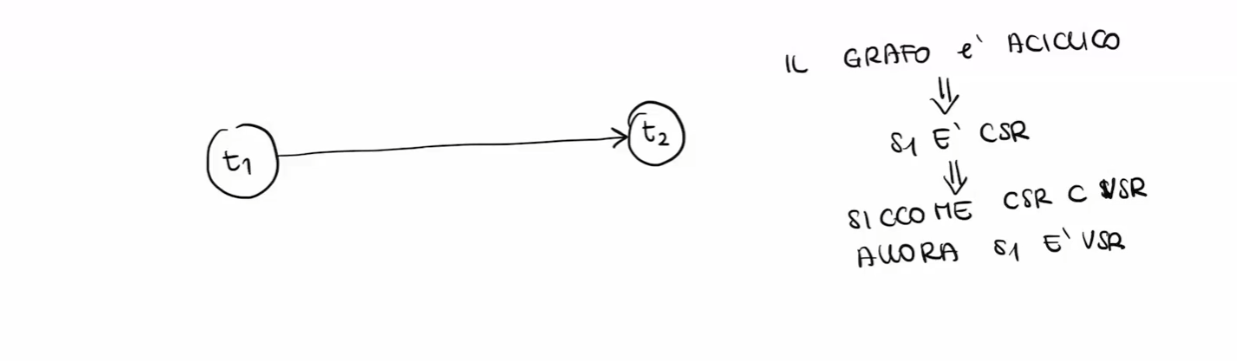
\includegraphics[width=1\linewidth]{image242}
	\label{fig:image242}
\end{figure}
Tutti e tre i conflitti generano archi nella stessa direzione $t_1 \to t_2$. Il grafo dei conflitti è quindi aciclico, pertanto $S_1$ è CSR. Poiché $\text{CSR} \subseteq \text{VSR}$, concludiamo che $\mathbf{S_1}$ \textbf{è sia CSR che VSR}.

\paragraph{Esempio CSR: schedule $S_2$.}

Riprendiamo lo schedule $S_2$ già analizzato in precedenza:
\[
S_2 : r_1(x),\ w_1(x),\ w_3(x),\ r_2(y),\ r_3(y),\ w_3(y),\ w_1(y),\ r_2(x)
\]

Costruiamo l'insieme dei conflitti:
\[
\text{CONFLITTI}(S_2) = \{
(r_1(x),\ w_3(x)),\
(w_1(x),\ w_3(x)),\
(w_1(x),\ r_2(x)),\
(w_3(x),\ r_2(x)),\
(r_2(y),\ w_3(y)),\
(r_2(y),\ w_1(y)),\
(r_3(y),\ w_1(y)),\
(w_3(y),\ w_1(y))
\}
\]

Ricaviamo gli archi del grafo dei conflitti:
\begin{itemize}
	\item $(r_1(x),\ w_3(x))$, $(w_1(x),\ w_3(x))$ $\Rightarrow$ arco $t_1 \to t_3$;
	\item $(w_1(x),\ r_2(x))$ $\Rightarrow$ arco $t_1 \to t_2$;
	\item $(w_3(x),\ r_2(x))$ $\Rightarrow$ arco $t_3 \to t_2$;
	\item $(r_2(y),\ w_3(y))$ $\Rightarrow$ arco $t_2 \to t_3$;
	\item $(r_2(y),\ w_1(y))$ $\Rightarrow$ arco $t_2 \to t_1$;
	\item $(r_3(y),\ w_1(y))$, $(w_3(y),\ w_1(y))$ $\Rightarrow$ arco $t_3 \to t_1$.
\end{itemize}

\begin{figure}[H]
	\centering
	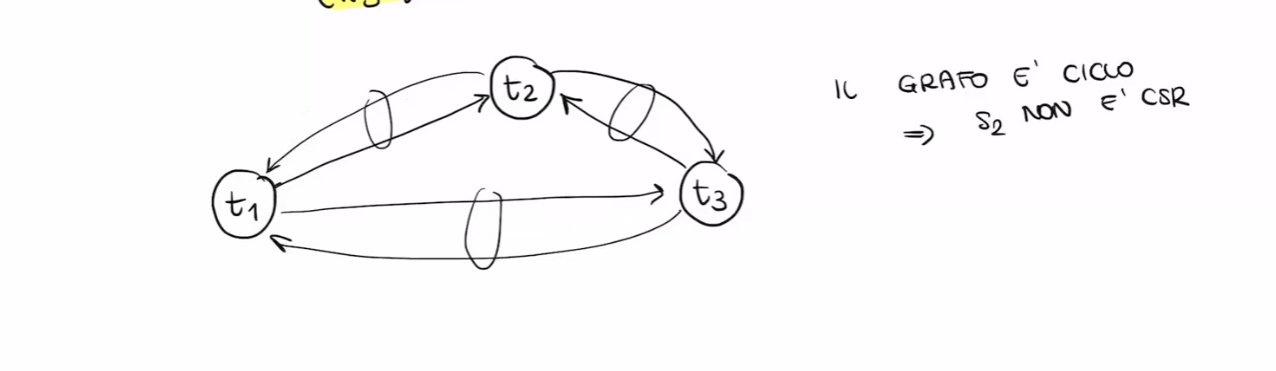
\includegraphics[width=1\linewidth]{image243}
	\label{fig:image243}
\end{figure}
Il grafo dei conflitti contiene cicli: $t_2 \to t_3 \to t_2$ e $t_1 \to t_3 \to t_1$. Il grafo è quindi ciclico, pertanto $S_2$ non è CSR. Poiché $\text{CSR} \subseteq \text{VSR}$ e avevamo già dimostrato che $S_2$ non è VSR, possiamo concludere che $\mathbf{S_2}$ \textbf{non è né CSR né VSR}.
\paragraph{Esempio CSR: schedule $S_3$.}

Riprendiamo lo schedule $S_3$ già analizzato in precedenza:
\[
S_3 : r_1(x),\ r_2(x),\ w_2(x),\ r_3(x),\ r_4(z),\ w_1(x),\ w_3(y),\ w_3(x),\ w_1(y),\ w_5(x),\ w_1(z),\ w_5(y),\ r_5(z)
\]

Costruiamo l'insieme dei conflitti:
\begin{align*}
	\text{CONFLITTI}(S_3) = \{
	&(r_1(x),\ w_2(x)),\ (r_1(x),\ w_3(x)),\ (r_1(x),\ w_5(x)), \\
	&(r_2(x),\ w_1(x)),\ (r_2(x),\ w_3(x)),\ (r_2(x),\ w_5(x)), \\
	&(w_2(x),\ r_3(x)),\ (w_2(x),\ w_1(x)),\ (w_2(x),\ w_3(x)),\ (w_2(x),\ w_5(x)), \\
	&(r_3(x),\ w_1(x)),\ (r_3(x),\ w_5(x)), \\
	&(r_4(z),\ w_1(z)), \\
	&(w_1(x),\ w_3(x)),\ (w_1(x),\ w_5(x)), \\
	&(w_1(y),\ w_5(y)), \\
	&(w_3(y),\ w_1(y)),\ (w_3(y),\ w_5(y)), \\
	&(w_3(x),\ w_5(x))
	\}
\end{align*}

Ricaviamo gli archi del grafo dei conflitti:
\begin{itemize}
	\item $(r_1(x),\ w_2(x))$ $\Rightarrow$ arco $t_1 \to t_2$;
	\item $(r_1(x),\ w_3(x))$, $(r_1(x),\ w_5(x))$ $\Rightarrow$ archi $t_1 \to t_3$, $t_1 \to t_5$;
	\item $(r_2(x),\ w_1(x))$ $\Rightarrow$ arco $t_2 \to t_1$;
	\item $(r_2(x),\ w_3(x))$, $(r_2(x),\ w_5(x))$ $\Rightarrow$ archi $t_2 \to t_3$, $t_2 \to t_5$;
	\item $(w_2(x),\ r_3(x))$, $(w_2(x),\ w_1(x))$, $(w_2(x),\ w_3(x))$, $(w_2(x),\ w_5(x))$ $\Rightarrow$ archi $t_2 \to t_3$, $t_2 \to t_1$, $t_2 \to t_3$, $t_2 \to t_5$;
	\item $(r_3(x),\ w_1(x))$, $(r_3(x),\ w_5(x))$ $\Rightarrow$ archi $t_3 \to t_1$, $t_3 \to t_5$;
	\item $(r_4(z),\ w_1(z))$ $\Rightarrow$ arco $t_4 \to t_1$;
	\item $(w_1(x),\ w_3(x))$, $(w_1(x),\ w_5(x))$ $\Rightarrow$ archi $t_1 \to t_3$, $t_1 \to t_5$;
	\item $(w_3(y),\ w_1(y))$ $\Rightarrow$ arco $t_3 \to t_1$;
	\item $(w_3(y),\ w_5(y))$, $(w_3(x),\ w_5(x))$ $\Rightarrow$ archi $t_3 \to t_5$;
	\item $(w_1(y),\ w_5(y))$ $\Rightarrow$ arco $t_1 \to t_5$.
\end{itemize}
\begin{figure}[H]
	\centering
	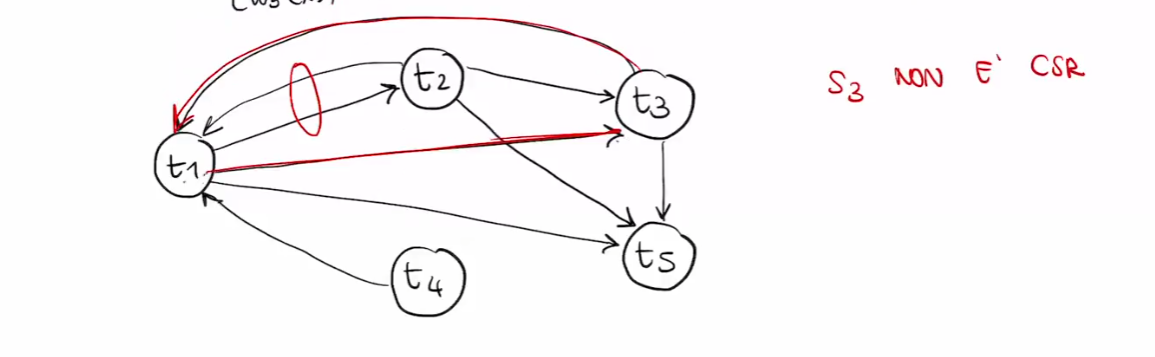
\includegraphics[width=0.7\linewidth]{image244}
	\label{fig:image244}
\end{figure}
Il grafo contiene cicli, ad esempio $t_1 \to t_2 \to t_1$ (dagli archi $t_1 \to t_2$ e $t_2 \to t_1$) e $t_2 \to t_3 \to t_1 \to t_2$. Il grafo è quindi ciclico, pertanto $S_3$ non è CSR. Poiché avevamo già dimostrato che $S_3$ non è VSR, concludiamo che $\mathbf{S_3}$ \textbf{non è né CSR né VSR}.
\paragraph{Esempio CSR: schedule $S_4$.}

Consideriamo lo schedule:
\[
S_4 : r_1(x),\ r_3(y),\ w_1(y),\ w_4(x),\ w_1(t),\ w_5(x),\ r_2(z),\ r_3(z),\ w_2(z),\ w_5(z),\ r_4(t),\ r_5(t)
\]

Costruiamo l'insieme dei conflitti:
\begin{align*}
	\text{CONFLITTI}(S_4) = \{
	&(r_1(x),\ w_4(x)),\ (r_1(x),\ w_5(x)), \\
	&(r_3(y),\ w_1(y)), \\
	&(w_4(x),\ w_5(x)), \\
	&(w_1(t),\ r_4(t)),\ (w_1(t),\ r_5(t)), \\
	&(r_2(z),\ w_5(z)), \\
	&(r_3(z),\ w_2(z)),\ (r_3(z),\ w_5(z)), \\
	&(w_2(z),\ w_5(z))
	\}
\end{align*}

Ricaviamo gli archi del grafo dei conflitti:
\begin{itemize}
	\item $(r_1(x),\ w_4(x))$, $(r_1(x),\ w_5(x))$ $\Rightarrow$ archi $t_1 \to t_4$, $t_1 \to t_5$;
	\item $(r_3(y),\ w_1(y))$ $\Rightarrow$ arco $t_3 \to t_1$;
	\item $(w_4(x),\ w_5(x))$ $\Rightarrow$ arco $t_4 \to t_5$;
	\item $(w_1(t),\ r_4(t))$, $(w_1(t),\ r_5(t))$ $\Rightarrow$ archi $t_1 \to t_4$, $t_1 \to t_5$;
	\item $(r_2(z),\ w_5(z))$ $\Rightarrow$ arco $t_2 \to t_5$;
	\item $(r_3(z),\ w_2(z))$, $(r_3(z),\ w_5(z))$ $\Rightarrow$ archi $t_3 \to t_2$, $t_3 \to t_5$;
	\item $(w_2(z),\ w_5(z))$ $\Rightarrow$ arco $t_2 \to t_5$.
\end{itemize}
\begin{figure}[H]
	\centering
	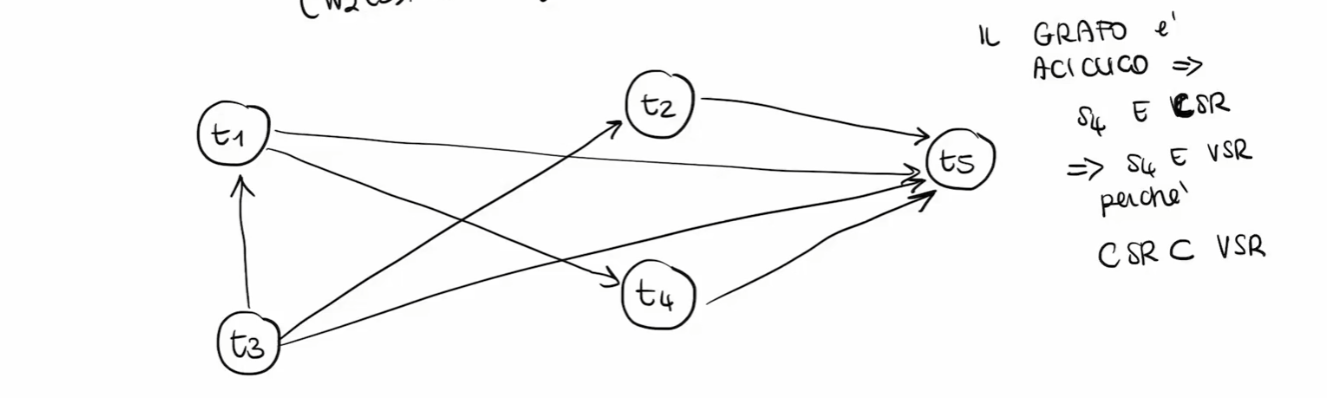
\includegraphics[width=0.7\linewidth]{image245}
	\caption{}
	\label{fig:image245}
\end{figure}
Il grafo dei conflitti ha quindi archi: $t_3 \to t_1 \to t_4 \to t_5$, $t_3 \to t_2 \to t_5$, $t_1 \to t_5$, $t_3 \to t_5$. Il grafo è \textbf{aciclico}, pertanto $S_4$ è CSR. Poiché $\text{CSR} \subseteq \text{VSR}$, concludiamo che $\mathbf{S_4}$ \textbf{è sia CSR che VSR}.
\paragraph{Ordinamenti topologici di $S_4$.}

Poiché il grafo dei conflitti di $S_4$ è aciclico, possiamo ricavare gli schedule seriali conflict-equivalenti tramite l'ordinamento topologico. Il nodo di partenza è $t_3$, l'unico senza archi entranti. I possibili ordinamenti topologici sono:

\begin{align*}
	S_{r1} &: t_3,\ t_1,\ t_5,\ t_2,\ t_4 \\
	S_{r2} &: t_3,\ t_1,\ t_5,\ t_4,\ t_2 \\
	S_{r3} &: t_3,\ t_2,\ t_1,\ t_4,\ t_5
\end{align*}

Tutti e tre gli schedule seriali sono conflict-equivalenti e view-equivalenti a $S_4$.
\subsection{Locking a due fasi stretto (2PL stretto)}

Il locking a due fasi stretto è il meccanismo principale per la gestione della concorrenza nei DBMS. I suoi vantaggi rispetto alla view-serializzabilità sono:
\begin{itemize}
	\item non richiede di conoscere in anticipo l'esito delle transazioni;
	\item fornisce un meccanismo base per la gestione dei lock;
	\item definisce una politica di concessione dei lock;
	\item garantisce la serializzabilità tramite una regola precisa.
\end{itemize}

\subsubsection{Meccanismo di base}

Per bloccare le risorse su cui si vuole operare si introducono le seguenti primitive di lock:
\begin{itemize}
	\item \textbf{R\_LOCK$_i(x)$}: la transazione $t_i$ richiede un lock condiviso in lettura sulla risorsa $x$;
	\item \textbf{W\_LOCK$_i(x)$}: la transazione $t_i$ richiede un lock esclusivo in scrittura sulla risorsa $x$;
	\item \textbf{UNLOCK$_i(x)$}: la transazione $t_i$ rilascia la risorsa $x$ da un precedente lock.
\end{itemize}

\paragraph{Regole d'uso delle primitive.}
\begin{itemize}
	\item Ogni operazione di \textbf{lettura} deve essere preceduta da una R\_LOCK e seguita da una UNLOCK. Sono ammessi più R\_LOCK contemporanei sulla stessa risorsa, poiché il lock in lettura è \textbf{condiviso}.
	\item Ogni operazione di \textbf{scrittura} deve essere preceduta da una W\_LOCK e seguita da una UNLOCK. Non sono ammessi più W\_LOCK contemporanei sulla stessa risorsa, poiché il lock in scrittura è \textbf{esclusivo}.
\end{itemize}

Una transazione che rispetta queste regole si dice \textbf{ben formata}.

\subsubsection{Politica di concessione dei lock}

Il gestore della concorrenza del DBMS mantiene per ogni risorsa $x$ le seguenti informazioni:
\begin{itemize}
	\item $\text{stato}(x) \in \{\text{libero},\ \text{r\_lock},\ \text{w\_lock}\}$: lo stato corrente della risorsa;
	\item $C(x) = \{t_1, \ldots, t_n\}$: l'insieme delle transazioni che detengono un R\_LOCK su $x$ (rilevante solo quando $\text{stato}(x) = \text{r\_lock}$).
\end{itemize}
\begin{figure}[H]
	\centering
	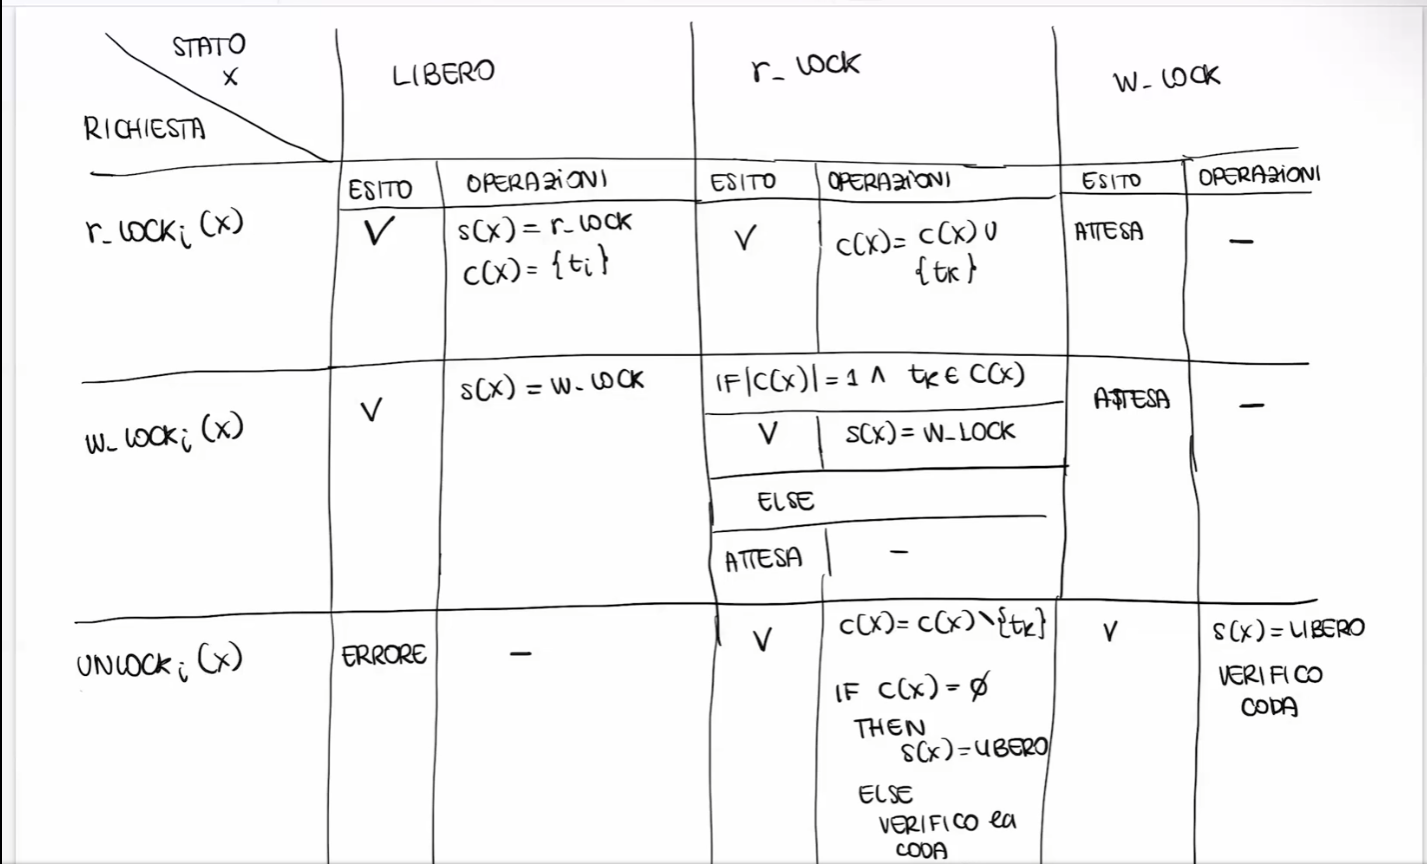
\includegraphics[width=1\linewidth]{image246}
	\caption{Tabella di concessione dei lock}
	\label{fig:image246}
\end{figure}
\subsection{Regola per la serializzabilità}

La regola da cui si ottiene la serializzabilità, e da cui deriva il nome \textit{2PL}, stabilisce che \textbf{una transazione, dopo aver rilasciato un lock, non può acquisirne altri}.

Il ciclo di vita di una transazione è suddiviso in due fasi distinte:

\begin{enumerate}
	\item \textbf{Fase di acquisizione (Growing Phase):} il numero di lock acquisiti cresce monotonicamente.
	\item \textbf{Fase di rilascio (Shrinking Phase):} il numero di lock decresce monotonicamente; non è più possibile acquisire nuovi lock.
\end{enumerate}

\begin{figure}[H]
	\centering
	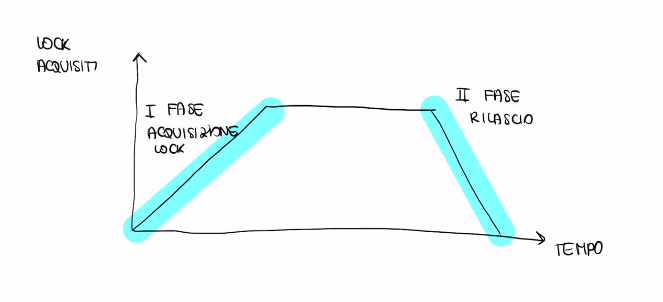
\includegraphics[width=1\linewidth]{image247}
	\caption{ciclo vita lock}
	\label{fig:image247}
\end{figure}

\paragraph{Esempio: perdita di aggiornamento con 2PL stretto.}

Consideriamo le transazioni:
\begin{align*}
	t_1 &: \text{R\_LOCK}_1(x),\ r_1(x),\ \text{W\_LOCK}_1(x),\ w_1(x),\ \text{UNLOCK}_1(x) \\
	t_2 &: \text{R\_LOCK}_2(x),\ r_2(x),\ \text{W\_LOCK}_2(x),\ w_2(x),\ \text{UNLOCK}_2(x)
\end{align*}

Lo schedule con perdita di aggiornamento era:
\[
S_{pa} : r_1(x),\ r_2(x),\ w_2(x),\ w_1(x)
\]

Con il 2PL stretto, introduciamo esplicitamente le operazioni di lock:
\[
S_{pa}^{2PL} : \text{R\_LOCK}_1(x),\ r_1(x),\ \text{R\_LOCK}_2(x),\ r_2(x),\ \text{W\_LOCK}_2(x)\ [\text{?}],\ \ldots
\]

Quando $t_2$ tenta di acquisire W\_LOCK$_2(x)$, lo stato della risorsa è:
\[
\text{stato}(x) = \texttt{r\_lock}, \quad C(x) = \{t_1,\ t_2\}
\]

Dalla tabella di concessione, W\_LOCK$_2(x)$ è concedibile solo se $C(x) = \{t_2\}$, ovvero se $t_1$ ha già rilasciato il proprio R\_LOCK$_1(x)$. Tuttavia:

\begin{itemize}
	\item Se $t_1$ rilascia R\_LOCK$_1(x)$, entra nella \textbf{fase discendente} del 2PL.
	\item Nella fase discendente, $t_1$ non può più acquisire nuovi lock.
	\item Ma $t_1$ deve ancora eseguire $w_1(x)$, che richiede W\_LOCK$_1(x)$: \textbf{impossibile}.
\end{itemize}

Il 2PL stretto impedisce quindi strutturalmente lo schedule $S_{pa}$: non esiste alcun modo di ordinare le operazioni di lock e unlock che rispetti contemporaneamente la regola del 2PL e consenta l'esecuzione di entrambe le scritture. La perdita di aggiornamento viene così \textbf{prevenuta}.
\subsubsection{2PL stretto}

Il \textbf{2PL stretto} aggiunge un vincolo ulteriore rispetto al 2PL base: una transazione può rilasciare i propri lock \textbf{esclusivamente dopo aver eseguito un commit o un rollback}. Il momento in cui inizia la fase discendente coincide quindi con il commit o l'abort della transazione.

Questo vincolo aggiuntivo permette di \textbf{eliminare l'ipotesi di commit-proiezione}: il 2PL stretto garantisce la serializzabilità anche in presenza di transazioni che terminano con un abort, senza dover assumere a priori l'esito delle transazioni.

\subsubsection{Relazione tra 2PL stretto, CSR e VSR}

I tre insiemi di schedule sono in relazione di inclusione stretta:
\[
\text{2PL stretto} \subsetneq \text{CSR} \subsetneq \text{VSR}
\]

\begin{itemize}
	\item Ogni schedule prodotto dal 2PL stretto è conflict-serializzabile, ma non tutti gli schedule CSR sono producibili dal 2PL stretto.
	\item Ogni schedule CSR è view-serializzabile, ma non tutti gli schedule VSR sono conflict-serializzabili.
\end{itemize}

Il 2PL stretto è quindi la condizione più restrittiva: sacrifica parte della concorrenza ammessa da CSR e VSR, ma in cambio offre un meccanismo \textbf{pratico, efficiente e privo di ipotesi sull'esito delle transazioni}.
\subsection{Blocco critico (Deadlock)}

Il \textbf{blocco critico} (o \textit{deadlock}) si verifica durante l'esecuzione concorrente di due o più transazioni quando si crea una situazione di attesa circolare:
\begin{itemize}
	\item $t_1$ detiene una risorsa di cui $t_2$ ha bisogno, ed è in attesa di una risorsa detenuta da $t_2$;
	\item $t_2$ detiene una risorsa di cui $t_1$ ha bisogno, ed è in attesa di una risorsa detenuta da $t_1$.
\end{itemize}
Nessuna delle due transazioni può proseguire.

\paragraph{Frequenza del deadlock.}
Assumendo una granularità del lock a livello di tupla e indicando con $N$ il numero medio di tuple per tabella, la probabilità di deadlock di lunghezza due è:
\[
P(\text{deadlock}) = \frac{1}{N^2}
\]
All'aumentare del numero di tuple la probabilità decresce: con granularità fine il deadlock è un evento raro.

\paragraph{Tecniche di gestione.}

\begin{enumerate}
	\item \textbf{Timeout}: una transazione in attesa di una risorsa viene abortita allo scadere di un intervallo di tempo prefissato. È la tecnica più semplice da implementare, ma può abortire transazioni che non sono effettivamente in deadlock.
	
	\item \textbf{Prevenzione}: ogni transazione acquisisce \textbf{tutte} le risorse di cui necessita in lettura e scrittura in un'unica soluzione, secondo una politica del tutto-o-niente. Elimina il deadlock alla radice, ma è molto costosa in termini di concorrenza, poiché le risorse vengono bloccate anche quando non sono ancora necessarie.
	
	\item \textbf{Rilevamento}: è la tecnica adottata nella maggior parte dei sistemi reali. Periodicamente il sistema analizza la tabella dei lock alla ricerca di cicli di attesa; se viene rilevato un deadlock, una delle transazioni coinvolte viene abortita per spezzare il ciclo. Lo svantaggio è il rischio di \textbf{starvation}: la stessa transazione potrebbe essere ripetutamente scelta come vittima e non riuscire mai a completare.
\end{enumerate}
\subsection{Livelli di isolamento}

Esiste un compromesso fondamentale tra il grado di isolamento dalle anomalie e le prestazioni del sistema (misurate in TPS): maggiore è il controllo della concorrenza, minore è il parallelismo ammesso e quindi le prestazioni. I DBMS consentono di rinunciare, in tutto o in parte, al controllo della concorrenza, specificando quali anomalie si è disposti a tollerare tramite i \textbf{livelli di isolamento}.

\begin{figure}[H]
	\centering
	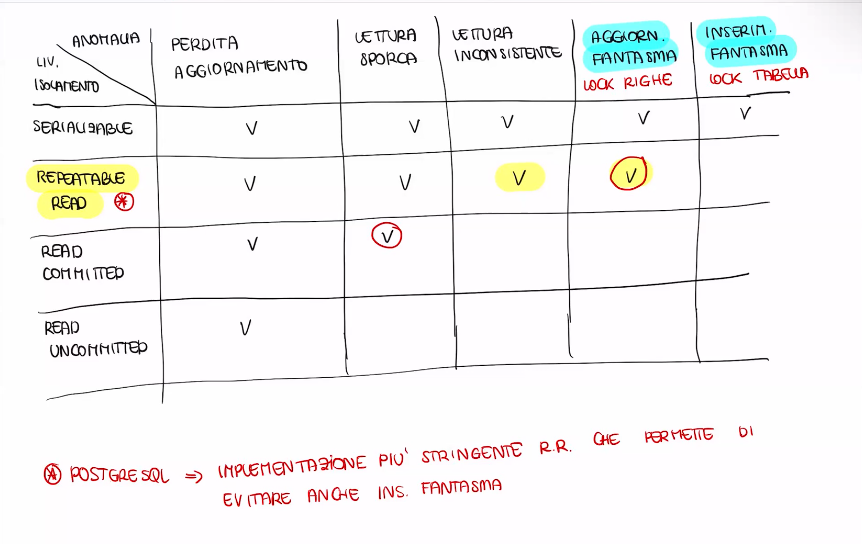
\includegraphics[width=1\linewidth]{image248}
	\caption{Anomalie evitate (\checkmark) per ciascun livello di isolamento}
	\label{fig:image248}
\end{figure}

\noindent$^*$ \textit{PostgreSQL} adotta un'implementazione più stringente del livello Repeatable Read, che permette di evitare anche l'inserimento fantasma.

Al livello più alto (\textbf{Serializable}) tutte le anomalie sono prevenute; scendendo di livello si tollerano anomalie via via più gravi, guadagnando in concorrenza e prestazioni.
\subsubsection{Implementazione dei livelli di isolamento}

Tutti i livelli di isolamento richiedono il \textbf{2PL stretto per le scritture}: i lock in scrittura vengono sempre rilasciati solo dopo il commit o il rollback. I livelli si differenziano invece nella gestione dei lock in lettura.

\begin{itemize}
	\item \textbf{Serializable}: applica il 2PL stretto anche per le letture e acquisisce lock a livello di \textbf{tabella}, prevenendo così l'anomalia di inserimento fantasma.
	
	\item \textbf{Repeatable Read}: applica il 2PL stretto anche per le letture, ma acquisisce lock a livello di \textbf{tupla} anziché di tabella. Previene la lettura inconsistente e l'aggiornamento fantasma, ma ammette l'anomalia di inserimento fantasma.
	
	\item \textbf{Read Committed}: acquisisce lock condivisi in lettura, ma \textbf{non} segue la regola del 2PL stretto per essi: i lock in lettura vengono rilasciati non appena l'operazione di lettura è completata, senza attendere il commit. Previene la lettura sporca, ma ammette la lettura inconsistente.
	
	\item \textbf{Read Uncommitted}: non acquisisce alcun lock in lettura. È il livello con la massima concorrenza, ma ammette tutte le anomalie di lettura, compresa la lettura sporca.
\end{itemize}
	\section{Linguaggio di Interrogazione SQL}

\textbf{SQL} (Structured Query Language) è il linguaggio di riferimento per la gestione delle \textbf{basi di dati relazionali}. 
In origine l'acronimo indicava \textit{Structured Query Language}, mentre oggi viene considerato semplicemente un \textbf{nome proprio}.

SQL è un linguaggio molto completo che permette di svolgere diverse operazioni su una base di dati.


SQL consente di:

\begin{itemize}
	\item Definire la struttura di una base di dati
	\item Modificare lo schema della base di dati
	\item Inserire, modificare e cancellare i dati
	\item Eseguire interrogazioni semplici
	\item Eseguire interrogazioni complesse (interrogazioni annidate, raggruppamenti, ecc.)
\end{itemize}

Per questo motivo SQL è diviso in diversi sottolinguaggi.

\begin{itemize}
	\item \textbf{DDL (Data Definition Language)}: permette di definire la struttura della base di dati e i vincoli di integrità.
	\item \textbf{DML (Data Manipulation Language)}: permette di inserire, modificare o cancellare i dati.
	\item \textbf{DQL (Data Query Language)}: permette di interrogare la base di dati tramite query.
\end{itemize}

SQL è un \textbf{linguaggio dichiarativo}.  
Questo significa che l'utente specifica \textbf{cosa vuole ottenere}, ma non \textbf{come} il sistema deve eseguire l'operazione.

Ad esempio, quando si scrive una query SQL, si indica semplicemente il risultato desiderato.

\begin{center}
	\texttt{SELECT nome FROM Studenti WHERE voto > 25}
\end{center}

Il modo in cui la query viene eseguita è deciso automaticamente dal \textbf{DBMS}.

Una componente del DBMS chiamata \textbf{query optimizer} traduce la query SQL in operazioni interne più efficienti.  
Questo processo è nascosto all'utente e permette di esprimere interrogazioni in modo \textbf{astratto e ad alto livello}.


Nel tempo sono state definite diverse versioni dello standard SQL.

\begin{itemize}
	\item \textbf{SQL-86}: prima standardizzazione del linguaggio
	\item \textbf{SQL-89}: introduzione dell'integrità referenziale
	\item \textbf{SQL-92 (SQL-2)}: estensione significativa del linguaggio
	\item \textbf{SQL:1999 (SQL-3)}: introduzione di concetti orientati agli oggetti, trigger e funzioni
	\item Versioni successive (2003, 2006, 2008, 2011, 2016): introduzione di nuove funzionalità come supporto XML, JSON e dati temporali
\end{itemize}

Le varie versioni dello standard hanno progressivamente ampliato le capacità del linguaggio, mantenendo comunque compatibilità con le versioni precedenti.
\subsection{Clausola SELECT}
\begin{figure}[H]
	\centering
	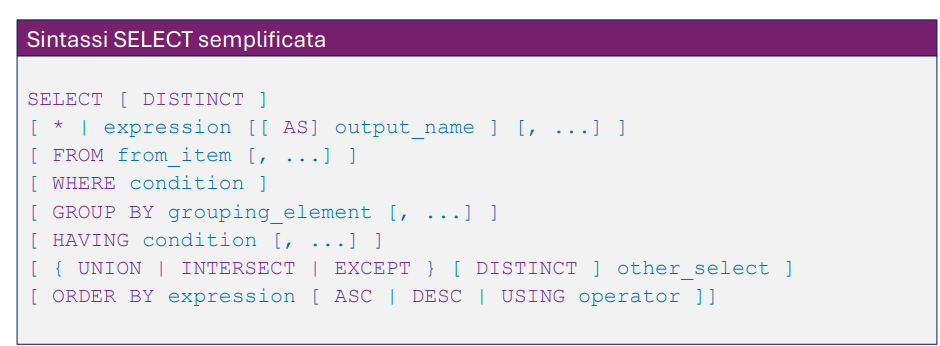
\includegraphics[width=1\linewidth]{image116}
	\caption{Sintassi SELECT}
	\label{fig:image116}
\end{figure}
\begin{itemize}
	\item \textbf{expression} è un’espressione che determina un attributo.
	\item \textbf{from\_item} è un’espressione che determina una sorgente per gli attributi.
	\item \textbf{condition} è un’espressione booleana utilizzata per selezionare i valori degli attributi.
	\item \textbf{grouping\_element} è un’espressione che permette di eseguire operazioni su più valori di un attributo e considerare il risultato complessivo.
\end{itemize}

\begin{figure}[H]
	\centering
	
\includegraphics[width=0.7\linewidth]{image117}
	\caption{Forma semplificata SELECT}
	\label{fig:image117}
\end{figure}


\begin{itemize}
	\item \textbf{SELECT}, \textbf{FROM} e \textbf{WHERE} sono chiamate \textbf{clausole}.
	\item La query estrae dal \textbf{prodotto cartesiano} delle tabelle elencate nella clausola \textbf{FROM} le righe che soddisfano la condizione specificata nella clausola \textbf{WHERE}.
	\item Il risultato dell’interrogazione è una \textbf{tabella} con una riga per ogni riga prodotta dalla clausola \textbf{FROM} ed eventualmente filtrata dalla clausola \textbf{WHERE} (se presente).
	\item Le colonne della tabella risultante dipendono dalla lista degli attributi specificata nella clausola \textbf{SELECT}.
\end{itemize}
\begin{figure}[H]
	\centering
	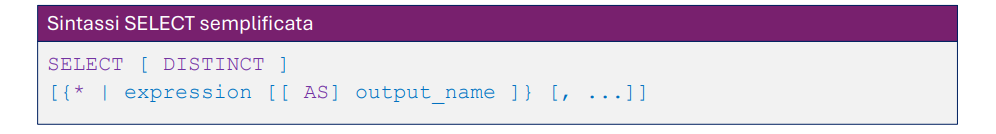
\includegraphics[width=1\linewidth]{image118}
	\caption{DISTINCT}
	\label{fig:image118}
\end{figure}
\begin{itemize}
	\item \textbf{*} è un’abbreviazione utilizzata per indicare tutti gli attributi delle tabelle.
	\item \textbf{expression} è un’espressione che coinvolge gli attributi della tabella (può anche essere semplicemente il nome di un attributo).
	\item \textbf{output\_name} è il nome assegnato all’attributo che conterrà il risultato della valutazione dell’espressione \textbf{expression} nella relazione risultato.
	\item \textbf{DISTINCT}: se presente richiede l’eliminazione delle tuple duplicate.
\end{itemize}
\begin{figure}[H]
	\centering
	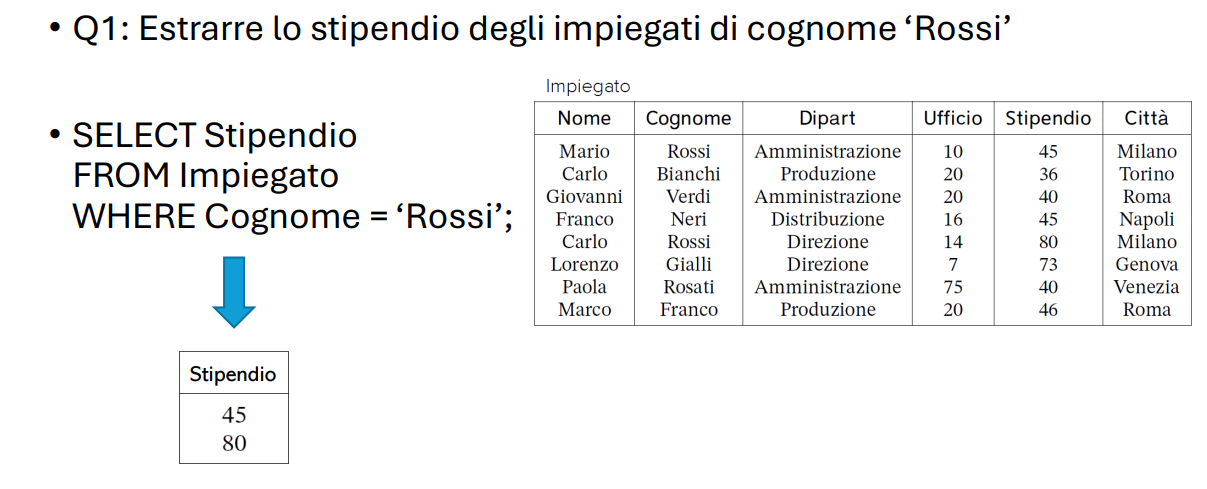
\includegraphics[width=1\linewidth]{image119}
	\caption{Esempio : Estrarre lo stipendio degli impiegati di cognome "Rossi"}
	\label{fig:image119}
\end{figure}
\begin{figure}[H]
	\centering
	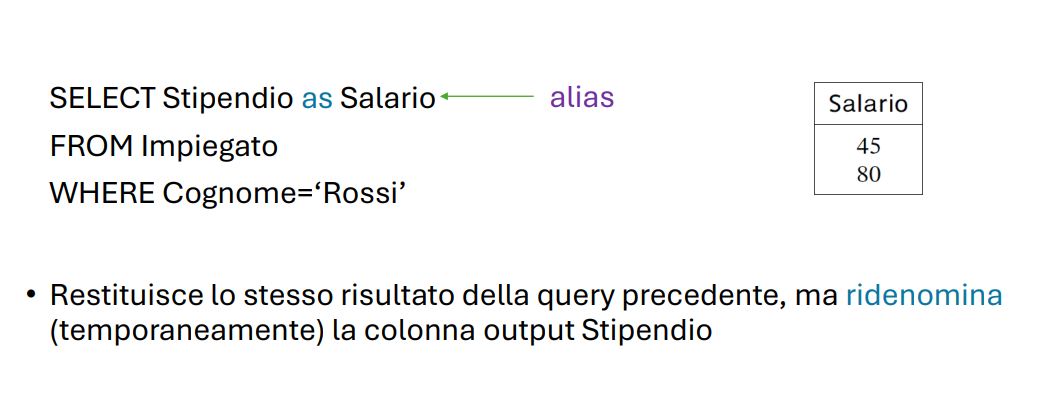
\includegraphics[width=1\linewidth]{image120}
	\caption{Uso di AS (ridenominazione)}
	\label{fig:image120}
\end{figure}
\begin{figure}[H]
	\centering
	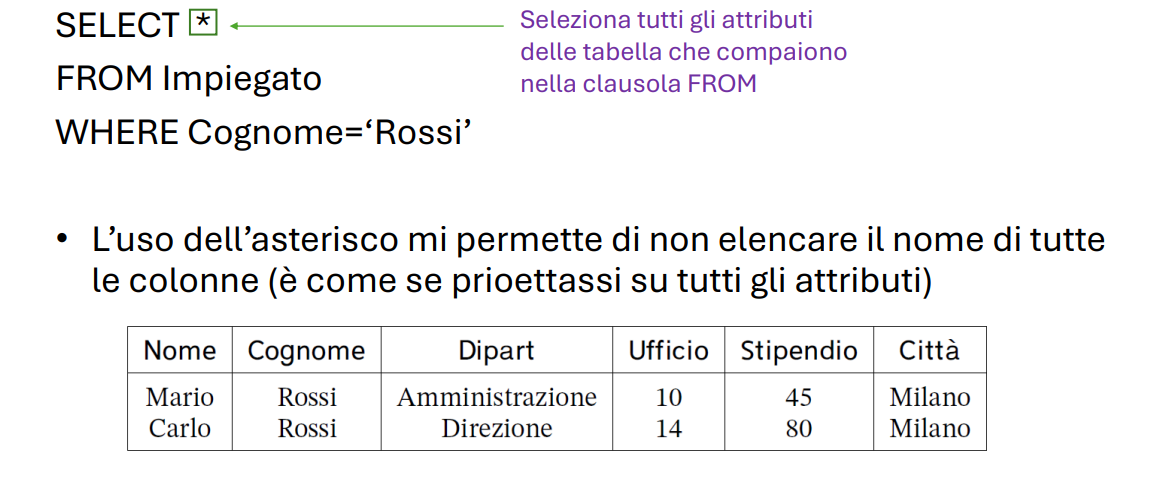
\includegraphics[width=1\linewidth]{image121}
	\caption{Uso dell'asterisco}
	\label{fig:image121}
\end{figure}
\subsection{Clausola FROM}
\begin{figure}[H]
	\centering
	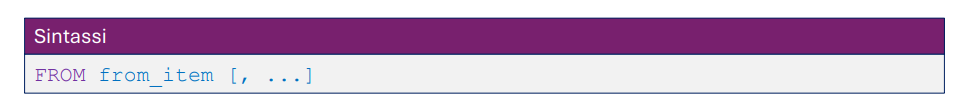
\includegraphics[width=1\linewidth]{image122}
	\caption{Sintassi FROM}
	\label{fig:image122}
\end{figure}
dove \textbf{from\_item} può essere una delle seguenti clausole (versione semplificata):

\begin{itemize}
	\item \textbf{table\_name [[AS] alias [(column\_alias [, ...])]]}
	
	Se sono presenti due o più tabelle, si esegue il \textbf{prodotto cartesiano} tra tutte le tabelle.  
	Se ci sono attributi con lo stesso nome su tabelle diverse, nella clausola \textbf{SELECT} questi attributi sono identificati anteponendo il nome della tabella e un punto:
	
	\begin{center}
		\texttt{nomeTabella.nomeAttributo}
	\end{center}
	
	\item \textbf{(other\_select) [AS] nomeRisultato [(column\_alias [, ...])]}
	
	È una \textbf{SELECT innestata}.  
	Il risultato della SELECT interna viene trattato come una tabella temporanea con nome \textbf{nomeRisultato}, sulla quale viene eseguita la SELECT esterna.
	
	\item \textbf{from\_item [NATURAL] join\_type from\_item [ON condition]}
	
	È la clausola \textbf{JOIN}.  
	
	Rappresenta un metodo più sofisticato rispetto al caso 1), che permette di selezionare un sottoinsieme del prodotto cartesiano di due o più tabelle.  
	Il parametro \textbf{join\_type} specifica il tipo di join da utilizzare. I principali tipi di join sono descritti nelle slide successive.
\end{itemize}
\begin{figure}[H]
	\centering
	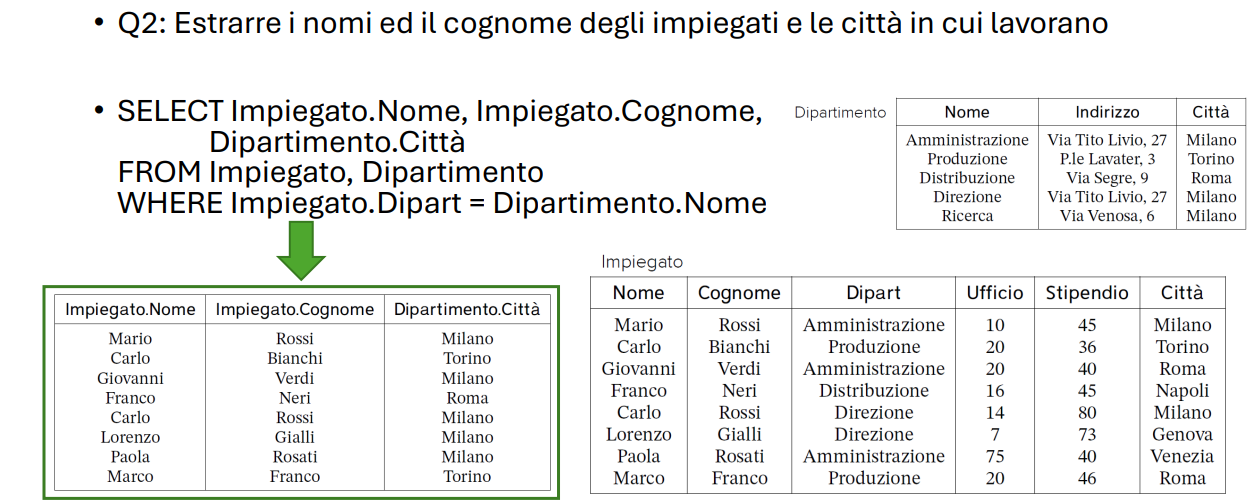
\includegraphics[width=1\linewidth]{image123}
	\caption{Estrarre i nomi ed il cognome degli impiegati e le città in cui lavorano}
	\label{fig:image123}
\end{figure}
\begin{figure}[H]
	\centering
	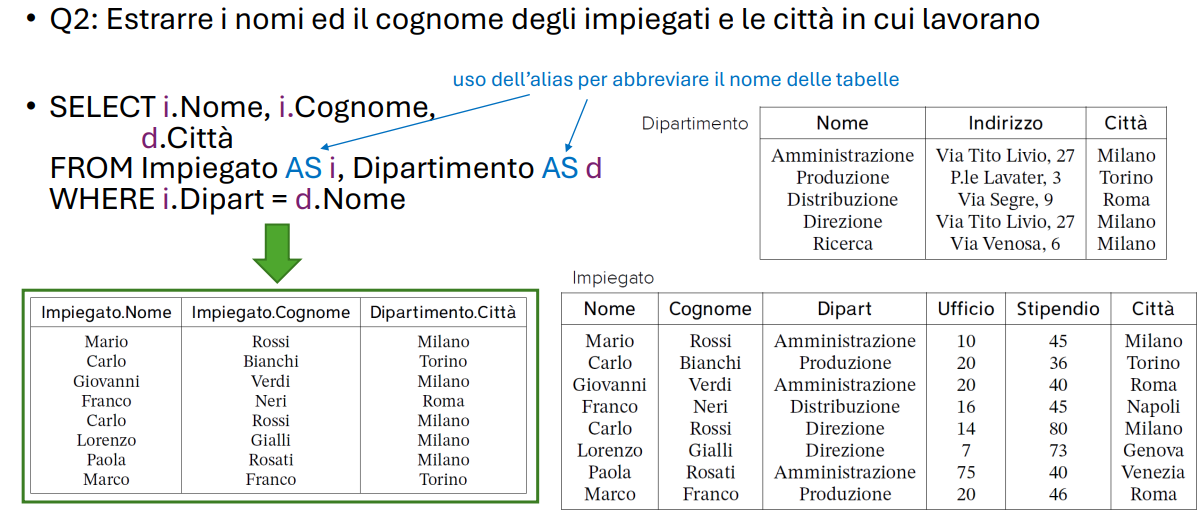
\includegraphics[width=1\linewidth]{image124}
	\caption{Stessa cosa di prima ma con AS}
	\label{fig:image124}
\end{figure}
\subsection{Clausola WHERE}
\begin{figure}[H]
	\centering
	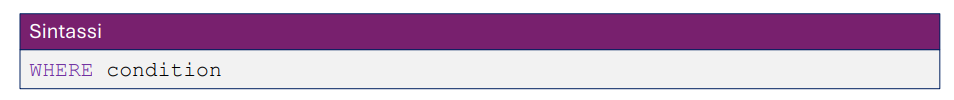
\includegraphics[width=1\linewidth]{image125}
	\caption{Sintassi WHERE}
	\label{fig:image125}
\end{figure}
\begin{itemize}
	\item La clausola \textbf{WHERE} ammette come argomento un’espressione booleana costruita combinando predicati semplici con gli operatori \textbf{AND}, \textbf{OR} e \textbf{NOT}.
	
	\item \textbf{AND}: seleziona le righe in cui tutti i predicati sono veri.
	
	\item \textbf{OR}: seleziona le righe in cui almeno un predicato è vero.
	
	\item \textbf{NOT}: seleziona le righe in cui il predicato è falso.
	
	\item Ciascun predicato semplice utilizza gli operatori \textbf{=}, \textbf{$<>$}, \textbf{$<$}, \textbf{$>$}, \textbf{$\leq$} e \textbf{$\geq$} per confrontare un’espressione costruita a partire dal valore di un attributo con un valore costante oppure con un’altra espressione.
	
	\item Per esprimere la precedenza tra gli operatori \textbf{AND} e \textbf{OR} si utilizzano le \textbf{parentesi}.
\end{itemize}
\begin{figure}[H]
	\centering
	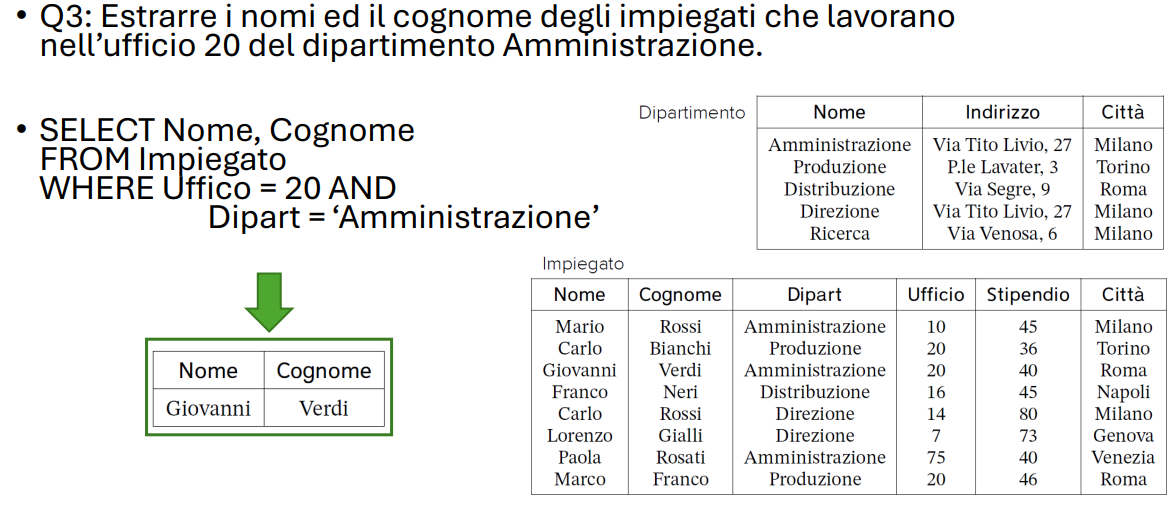
\includegraphics[width=1\linewidth]{image126}
	\caption{Estrarre i nomi ed il cognome degli impiegati che lavorano nell'ufficio 20 del dipartimento Amministrazione}
	\label{fig:image126}
\end{figure}
\begin{figure}[H]
	\centering
	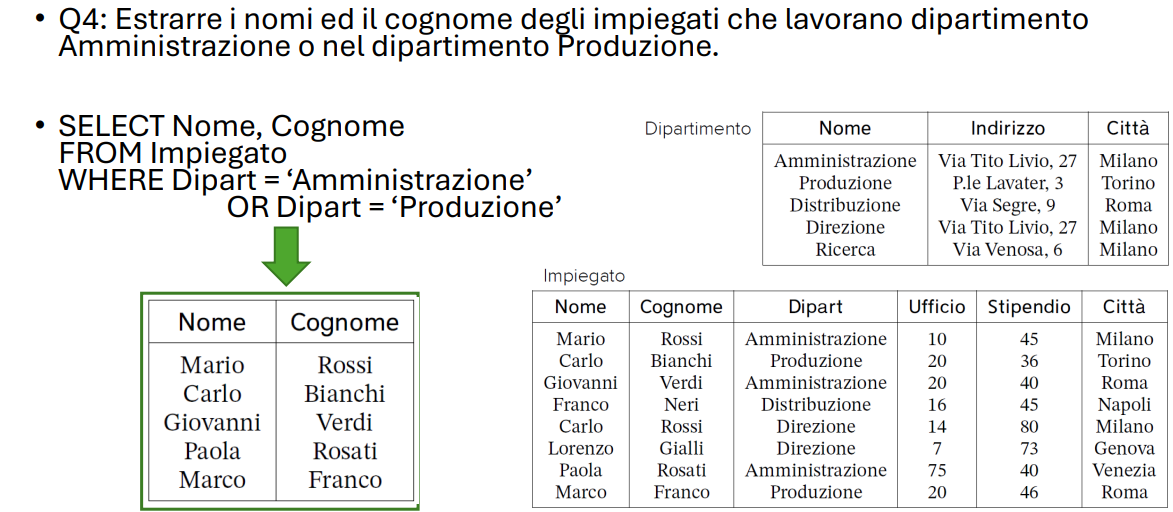
\includegraphics[width=1\linewidth]{image127}
	\caption{Estrarre i nomi ed il cognome degli impiegati che lavorano dipartimento Amministrazione o nel dipartimento Produzione.}
	\label{fig:image127}
\end{figure}
\begin{figure}[H]
	\centering
	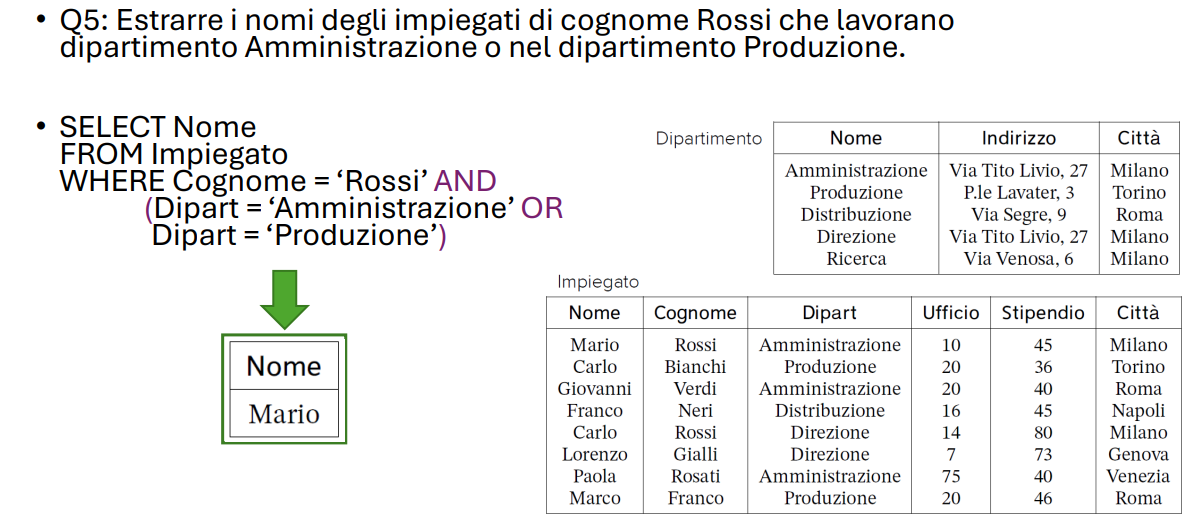
\includegraphics[width=1\linewidth]{image128}
	\caption{Estrarre i nomi degli impiegati di cognome Rossi che lavorano dipartimento Amministrazione o nel dipartimento Produzione.}
	\label{fig:image128}
\end{figure}
\subsubsection{Operatore LIKE}
\begin{itemize}
	\item Per il confronto tra stringhe, SQL mette a disposizione anche l’operatore \textbf{LIKE}, che consente di verificare se una stringa rispetta un certo \textbf{pattern} (oppure \textbf{ILIKE} per confronti \textit{case insensitive}).
	
	\item Due caratteri speciali utilizzati nei pattern sono \textbf{\_} e \textbf{\%}:
	
	\begin{itemize}
		\item \textbf{\_}: rappresenta un singolo carattere arbitrario.
		\item \textbf{\%}: rappresenta una sequenza di lunghezza arbitraria (anche nulla) di caratteri arbitrari.
	\end{itemize}
	
	\item Ad esempio:
	
	\begin{center}
		\texttt{\_o\%i}
	\end{center}
	
	rappresenta una stringa che ha una \textbf{o} in seconda posizione, seguita da una sequenza qualsiasi di caratteri (anche vuota) e che termina con una \textbf{i}.
\end{itemize}
\begin{figure}[H]
	\centering
	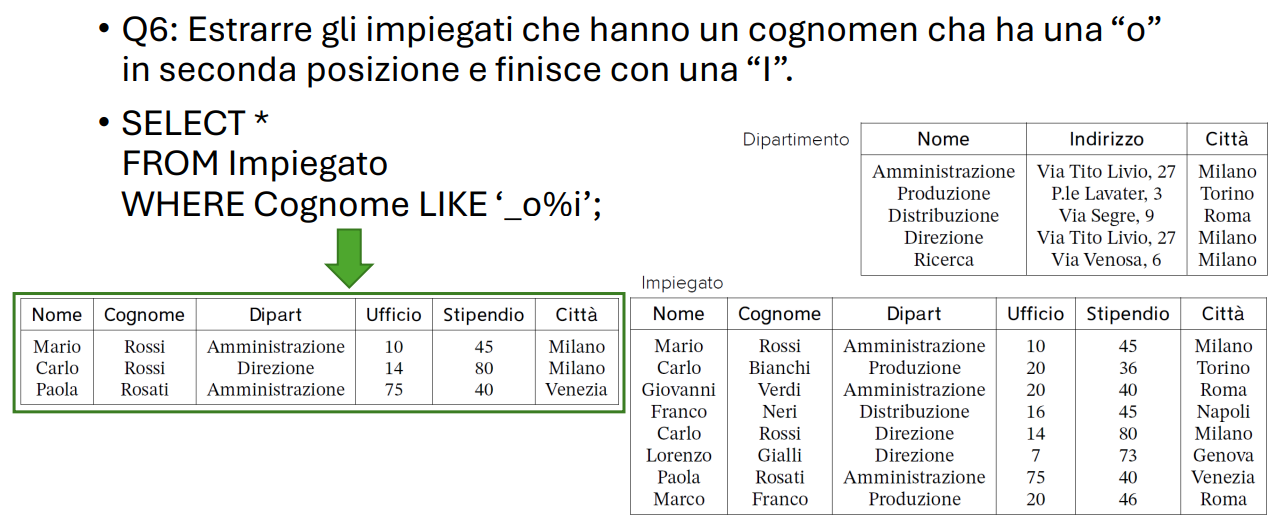
\includegraphics[width=1\linewidth]{image129}
	\caption{Estrarre gli impiegati che hanno un cognomen cha ha una “o” in seconda posizione e finisce con una “I”.}
	\label{fig:image129}
\end{figure}
\subsubsection{Operatore SIMILAR TO}
L'operatore \textbf{SIMILAR TO} è una versione più espressiva dell'operatore \textbf{LIKE}.  
Permette di confrontare stringhe utilizzando un \textbf{pattern} basato su un sottoinsieme delle 
\textbf{espressioni regolari POSIX} nella versione prevista dallo standard SQL.

Questo operatore consente quindi di effettuare confronti più avanzati rispetto a \texttt{LIKE}, 
utilizzando operatori tipici delle espressioni regolari.

\begin{itemize}
	
	\item \texttt{\_} : rappresenta \textbf{un singolo carattere qualsiasi}.
	
	\item \texttt{\%} : rappresenta \textbf{una sequenza di zero o più caratteri qualsiasi}.
	
	\item \texttt{*} : indica la \textbf{ripetizione del match precedente zero o più volte}.
	
	\item \texttt{+} : indica la \textbf{ripetizione del match precedente una o più volte}.
	
	\item \texttt{\{n,m\}} : indica la \textbf{ripetizione del match precedente almeno $n$ volte e al massimo $m$ volte}.
	
	\item \texttt{[...]} : rappresenta un \textbf{insieme di caratteri ammessi}; il match è valido se il carattere appartiene all'insieme specificato.
	
\end{itemize}
\begin{figure}[H]
	\centering
	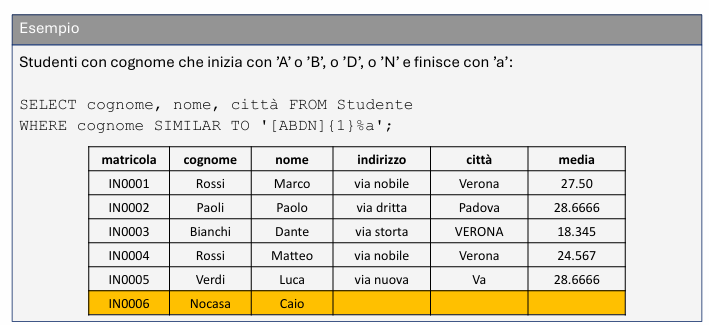
\includegraphics[width=1\linewidth]{image130}
	\caption{Esempio SIMILAR TO}
	\label{fig:image130}
\end{figure}
\subsubsection{Operatore BETWEEN}
L'operatore \textbf{BETWEEN} permette di verificare se il valore di un attributo  è compreso tra due valori estremi.
\begin{figure}[H]
	\centering
	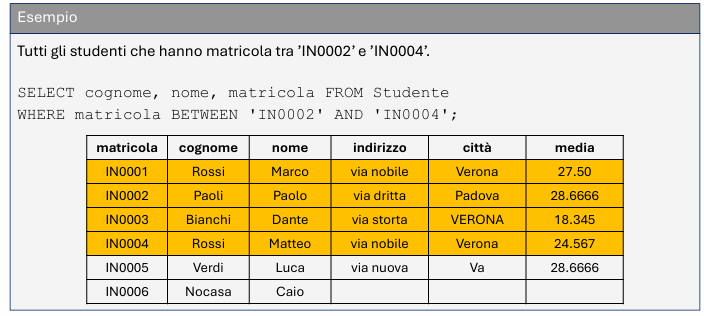
\includegraphics[width=1\linewidth]{image131}
	\caption{Esempio Between}
	\label{fig:image131}
\end{figure}
\begin{figure}[H]
	\centering
	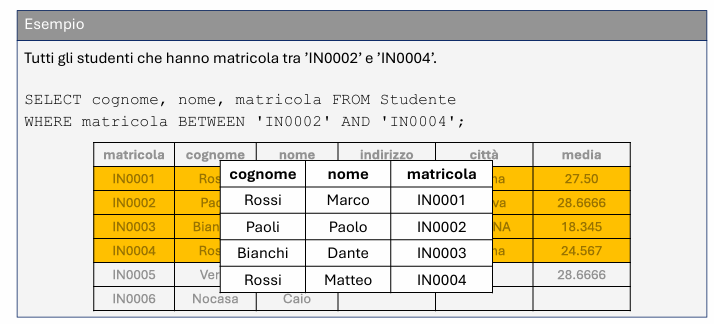
\includegraphics[width=1\linewidth]{image132}
	\caption{Esempio 2 di Between}
	\label{fig:image132}
\end{figure}
\subsubsection{Operatore IN}
Nella clausola \textbf{WHERE} può essere utilizzato l'operatore \textbf{[NOT] IN} 
per verificare se il valore di un attributo appartiene ad un insieme di valori.
\begin{figure}[H]
	\centering
	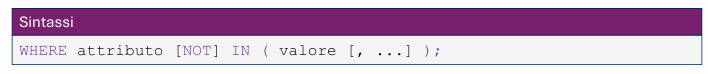
\includegraphics[width=1\linewidth]{image133}
	\caption{Sintassi IN}
	\label{fig:image133}
\end{figure}
\begin{figure}[H]
	\centering
	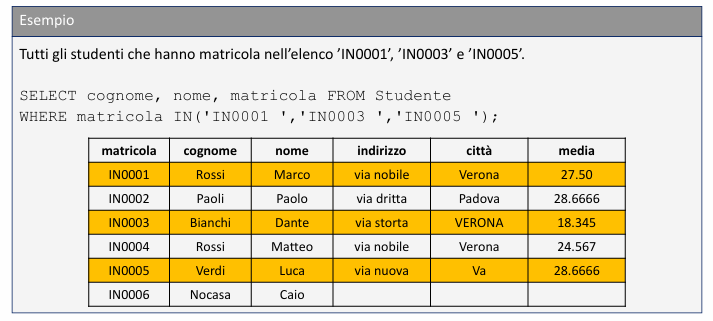
\includegraphics[width=1\linewidth]{image134}
	\caption{Esempio Operatore IN}
	\label{fig:image134}
\end{figure}
\subsubsection{Operatore IS NULL}
Per verificare se un attributo ha un valore nullo oppure no si utilizza il predicato 
\textbf{IS NULL}.

\begin{itemize}
	
	\item \texttt{attributo IS NULL}: restituisce \textbf{true} se l'attributo ha valore nullo.
	
	\item \texttt{attributo IS NOT NULL}: è la negazione del predicato precedente e restituisce 
	\textbf{true} se l'attributo ha un valore diverso da \texttt{NULL}.
	
\end{itemize}
\begin{figure}[H]
	\centering
	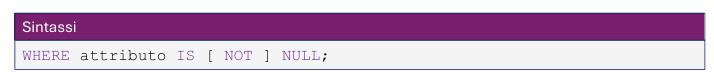
\includegraphics[width=1\linewidth]{image135}
	\caption{Sintassi IS NULL}
	\label{fig:image135}
\end{figure}
\begin{figure}[H]
	\centering
	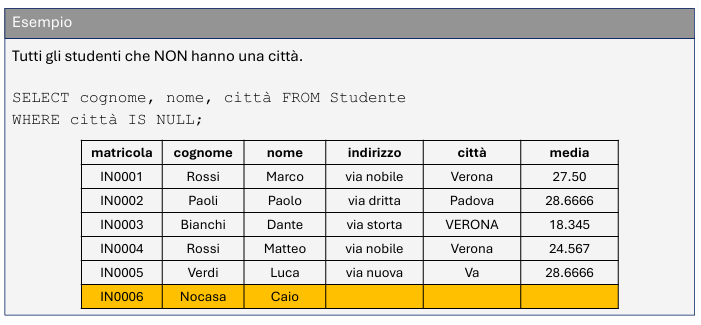
\includegraphics[width=1\linewidth]{image136}
	\caption{Esempio IS NULL}
	\label{fig:image136}
\end{figure}
\subsection{SQL e Algebra Relazionale}
Vediamo ora alcuni esempi di interrogazioni in \textbf{SQL} e analizziamo 
la loro corrispondenza con le equivalenti interrogazioni procedurali 
espresse tramite l'\textbf{algebra relazionale}.

L'obiettivo è comprendere come le interrogazioni dichiarative scritte in SQL 
possano essere interpretate come una sequenza di operazioni dell'algebra 
relazionale, che descrivono in modo procedurale i passi necessari per 
ottenere il risultato desiderato.
\begin{figure}[H]
	\centering
	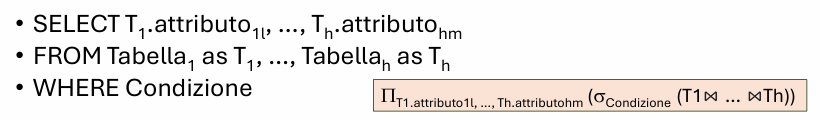
\includegraphics[width=1\linewidth]{image137}
	\caption{Sintassi algebra relazione e sql}
	\label{fig:image137}
\end{figure}
Nel caso di condizioni più complesse, la formula di conversione tra una
interrogazione \textbf{SQL} e la corrispondente espressione in
\textbf{algebra relazionale} non è sempre direttamente rappresentabile.

Una condizione fondamentale per poter effettuare questa conversione è
che l'interrogazione SQL utilizzi solo operatori che esistono anche
nell'algebra relazionale.

Se l'interrogazione SQL utilizza operatori non presenti nell'algebra
relazionale (ad esempio \textbf{operatori aggregati} come
\texttt{COUNT}, \texttt{SUM}, \texttt{AVG}, ecc.), la conversione
diretta non è possibile.
\begin{figure}[H]
	\centering
	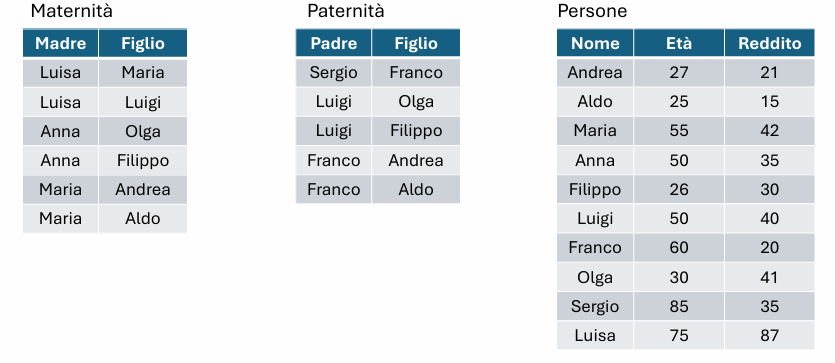
\includegraphics[width=1\linewidth]{image138}
	\caption{Tabella usata per gli esempi}
	\label{fig:image138}
\end{figure}
\subsection{SELECT}
\begin{figure}[H]
	\centering
	
\includegraphics[width=1\linewidth]{image139}
	\caption{}
	\label{fig:image139}
\end{figure}
\subsubsection{SELECT : alias di tabella o di attributo}
\begin{figure}[H]
	\centering
	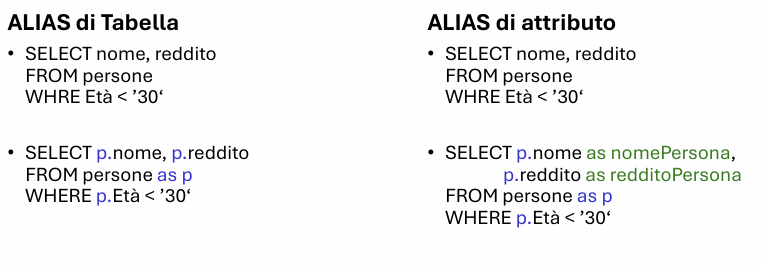
\includegraphics[width=1\linewidth]{image140}
	\caption{SELECT : alias di tabella o di attributo}
	\label{fig:image140}
\end{figure}
\subsubsection{SELECT: senza proiezione}
\begin{figure}[H]
	\centering
	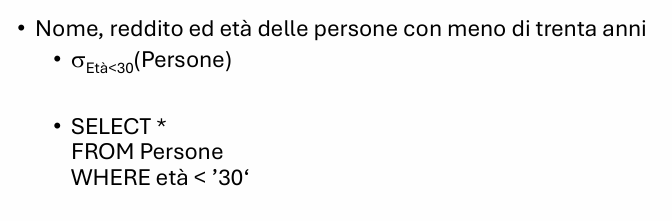
\includegraphics[width=1\linewidth]{image141}
	\caption{SELECT senza proiezione}
	\label{fig:image141}
\end{figure}
\subsubsection{Proiezione:gestione dei duplicati in SQL}

Una differenza significativa tra \textbf{SQL} e l'\textbf{algebra relazionale}
riguarda la gestione dei duplicati.

Nell'algebra relazionale i risultati delle operazioni sono considerati
\textbf{insiemi} e quindi non possono contenere duplicati.
In SQL, invece, i risultati sono trattati come \textbf{multinsiemi}
(\textit{bag}), per cui le righe duplicate possono essere presenti.

L'eliminazione delle righe duplicate è un'operazione computazionalmente
costosa; per questo motivo, \textbf{SQL mantiene i duplicati per default}.

Il costrutto \texttt{DISTINCT}, utilizzato dopo la parola chiave
\texttt{SELECT}, permette di eliminare le righe duplicate dal risultato.

Il costrutto \texttt{ALL} permette invece di mantenere esplicitamente
i duplicati, anche se questa è già la scelta predefinita del linguaggio SQL.
\begin{figure}[H]
	\centering
	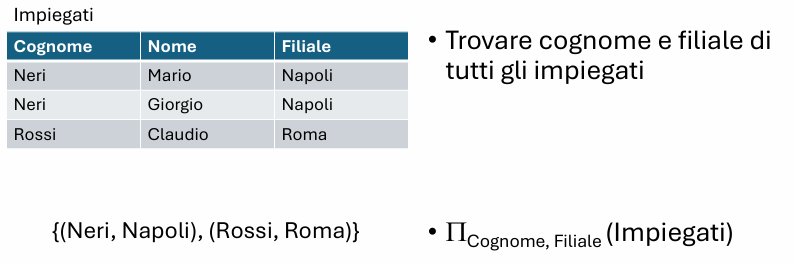
\includegraphics[width=1\linewidth]{image142}
	\caption{Proiezione: gestione dei duplicati in SQL}
	\label{fig:image142}
\end{figure}
\begin{figure}[H]
	\centering
	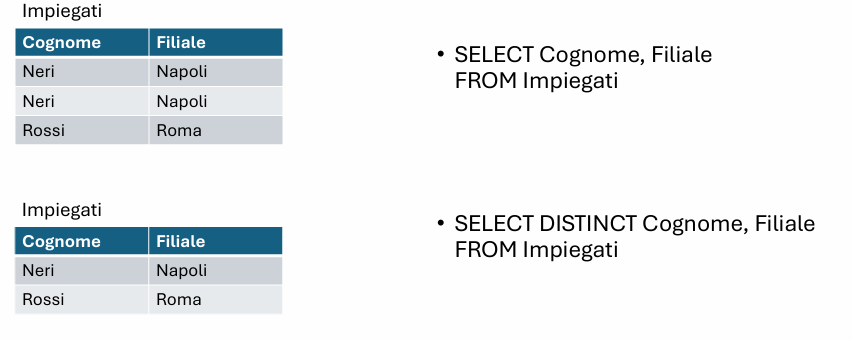
\includegraphics[width=1\linewidth]{image143}
	\caption{}
	\label{fig:image143}
\end{figure}
\begin{figure}[H]
	\centering
	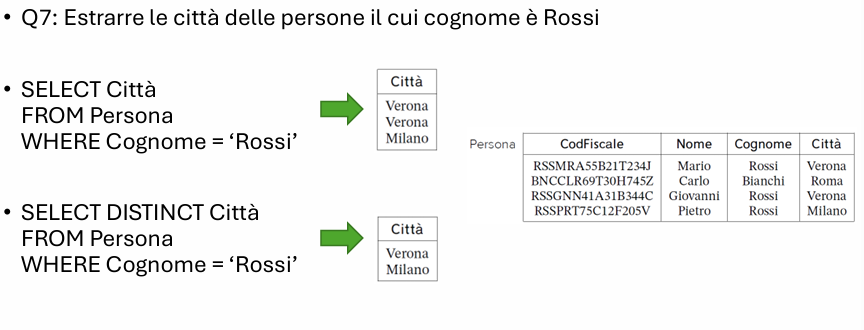
\includegraphics[width=1\linewidth]{image144}
	\caption{Esempio : gestione dei duplicati in SQL}
	\label{fig:image144}
\end{figure}
\subsubsection{SELECT: Selezione,Proiezione,Join}
L'istruzione \textbf{SELECT} permette di esprimere diverse operazioni
dell'\textbf{algebra relazionale}, a seconda della struttura
dell'interrogazione.

\begin{itemize}
	
	\item Con \textbf{una sola relazione} nella clausola \texttt{FROM} è possibile
	realizzare:
	\begin{itemize}
		\item \textbf{selezioni} ($\sigma$)
		\item \textbf{proiezioni} ($\pi$)
		\item \textbf{ridenominazioni} ($\rho$), utilizzando il costrutto \texttt{AS}
	\end{itemize}
	
	\item Con \textbf{più relazioni} nella clausola \texttt{FROM} si possono
	realizzare:
	\begin{itemize}
		\item \textbf{join} ($\bowtie$)
		\item \textbf{prodotti cartesiani}
	\end{itemize}
	
\end{itemize}

Le principali corrispondenze tra le clausole SQL e le operazioni
dell'algebra relazionale sono:

\begin{itemize}
	
	\item \texttt{SELECT} $\rightarrow$ $\pi$ \textbf{Proiezione} + $\rho$ \textbf{Ridenominazione}
	
	\item \texttt{FROM} $\rightarrow$ $\bowtie$ \textbf{Join} (prodotto cartesiano)
	
	\item \texttt{WHERE} $\rightarrow$ $\sigma$ \textbf{Selezione} + $\bowtie$ \textbf{Join} (condizione)
	
\end{itemize}
\subsection{Interrogazioni con JOIN}
In \textbf{SQL} il \textbf{join} può essere definito in due modi diversi.

\begin{itemize}
	
	\item Il primo metodo non richiede l'uso di una nuova sintassi: il legame tra
	le tabelle coinvolte viene specificato nella clausola \texttt{WHERE}.
	
	\item Il secondo metodo utilizza invece una sintassi dedicata all'interno
	della clausola \texttt{FROM}. In questo caso il join viene espresso
	esplicitamente tramite gli operatori di join.
	
\end{itemize}

Nel seguito verrà utilizzato il secondo approccio.
La clausola \textbf{FROM} ammette come argomento:

\begin{center}
	\texttt{table\_name [[AS] name] [, ...]}
\end{center}

Se nella clausola \texttt{FROM} sono presenti due o più nomi di tabelle,
viene eseguito il \textbf{prodotto cartesiano} tra tutte le tabelle.
Lo schema del risultato può quindi contenere tutti gli attributi
derivanti dal prodotto cartesiano delle relazioni coinvolte.

Il prodotto cartesiano tra due o più tabelle è chiamato
\textbf{CROSS JOIN}.

A partire dallo standard \textbf{SQL-2}, sono stati introdotti
altri tipi di join (\textit{join\_type}), tra cui:

\begin{itemize}
	\item \textbf{INNER JOIN}
	\item \textbf{LEFT [OUTER] JOIN}
	\item \textbf{RIGHT [OUTER] JOIN}
	\item \textbf{FULL [OUTER] JOIN}
\end{itemize}
\begin{figure}[H]
	\centering
	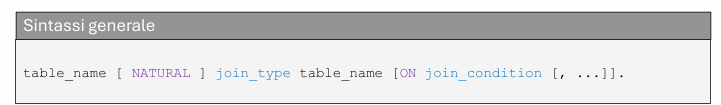
\includegraphics[width=1\linewidth]{image145}
	\caption{Sintassi JOIN}
	\label{fig:image145}
\end{figure}
dove \textit{join\_condition} è un'espressione booleana che seleziona le tuple
del join da aggiungere al risultato.

Le tuple selezionate possono essere successivamente filtrate
mediante la condizione specificata nella clausola \texttt{WHERE}.
\begin{figure}[H]
	\centering
	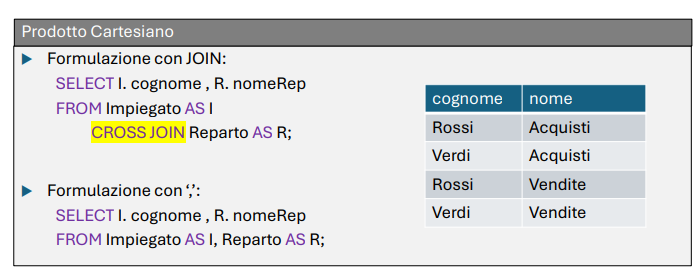
\includegraphics[width=1\linewidth]{image146}
	\caption{Prodotto cartesiano}
	\label{fig:image146}
\end{figure}
\subsubsection{INNER JOIN}
\begin{figure}[H]
	\centering
	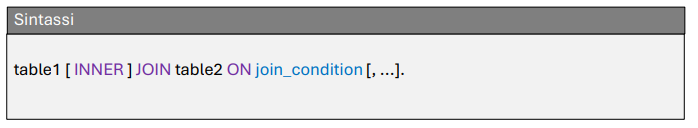
\includegraphics[width=1\linewidth]{image147}
	\caption{Sintassi INNER JOIN}
	\label{fig:image147}
\end{figure}
L'\textbf{INNER JOIN} rappresenta il tradizionale $\theta$-join dell’algebra relazionale.
Combina ciascuna riga $r_1$ della \texttt{table1} con ciascuna riga della \texttt{table2}
che soddisfa la condizione specificata nella clausola \texttt{ON}.
\begin{figure}[H]
	\centering
	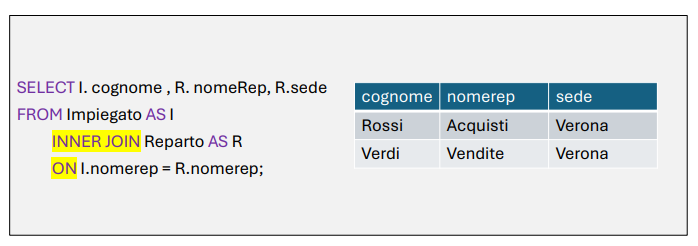
\includegraphics[width=1\linewidth]{image148}
	\caption{Esempio INNER JOIN}
	\label{fig:image148}
\end{figure}
\subsubsection{LEFT OUTER JOIN}
\begin{figure}[H]
	\centering
	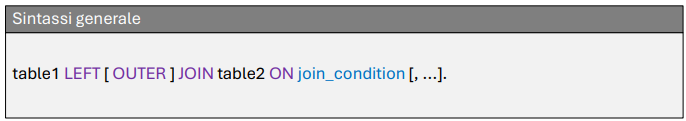
\includegraphics[width=1\linewidth]{image149}
	\caption{Sintassi LEFT OUTER JOIN}
	\label{fig:image149}
\end{figure}
Il \textbf{LEFT OUTER JOIN} esegue prima un \texttt{INNER JOIN}. 
Successivamente, per ogni riga della \texttt{table1} che non trova 
corrispondenza nella \texttt{table2}, viene comunque inserita nel risultato 
una riga contenente i valori della \texttt{table1} e \texttt{NULL} negli 
attributi della \texttt{table2}.
\begin{figure}[H]
	\centering
	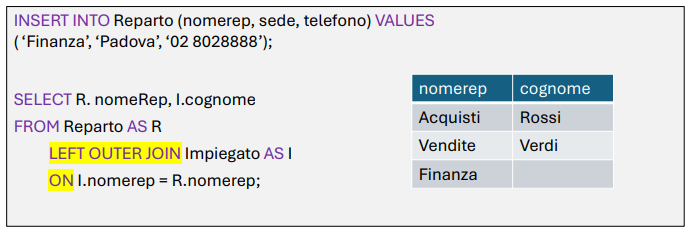
\includegraphics[width=1\linewidth]{image150}
	\caption{Esempio}
	\label{fig:image150}
\end{figure}
\begin{figure}[H]
	\centering
	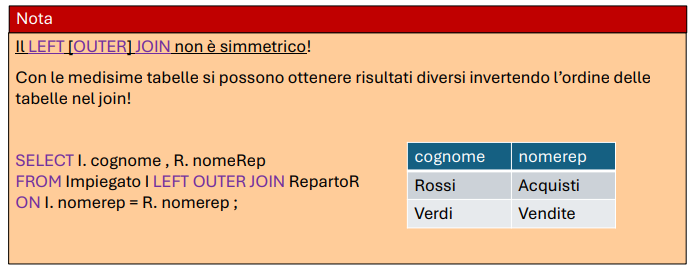
\includegraphics[width=1\linewidth]{image151}
	\caption{Nota}
	\label{fig:image151}
\end{figure}
\subsubsection{RIGHT OUTER JOIN}
\begin{figure}[H]
	\centering
	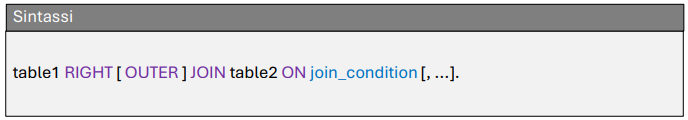
\includegraphics[width=1\linewidth]{image152}
	\caption{Sintassi RIGHT OUTER JOIN}
	\label{fig:image152}
\end{figure}
Il \textbf{RIGHT OUTER JOIN} esegue prima un \texttt{INNER JOIN}. 
Successivamente, per ogni riga della \texttt{table2} che non trova 
corrispondenza nella \texttt{table1}, viene comunque inserita nel risultato 
una riga contenente i valori della \texttt{table2} e \texttt{NULL} negli 
attributi della \texttt{table1}.
\begin{figure}[H]
	\centering
	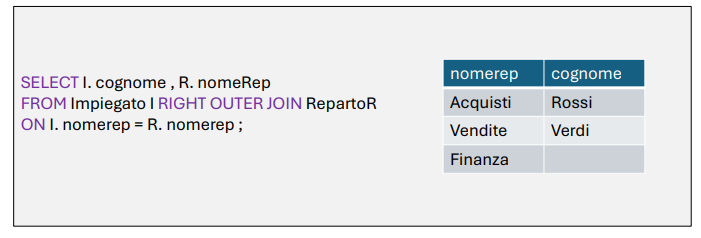
\includegraphics[width=1\linewidth]{image153}
	\caption{Esempio RIGHT OUTER JOIN}
	\label{fig:image153}
\end{figure}
\subsubsection{FULL OUTER JOIN}
\begin{figure}[H]
	\centering
	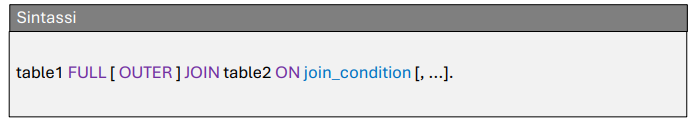
\includegraphics[width=1\linewidth]{image154}
	\caption{FULL OUTER JOIN}
	\label{fig:image154}
\end{figure}
Il \textbf{FULL OUTER JOIN} restituisce tutte le tuple prodotte da un 
\texttt{INNER JOIN}, più le tuple della prima tabella che non trovano 
corrispondenza nella seconda (come nel \texttt{LEFT OUTER JOIN}) e le 
tuple della seconda tabella che non trovano corrispondenza nella prima 
(come nel \texttt{RIGHT OUTER JOIN}). 

Non è equivalente a un \texttt{CROSS JOIN}.
\begin{figure}[H]
	\centering
	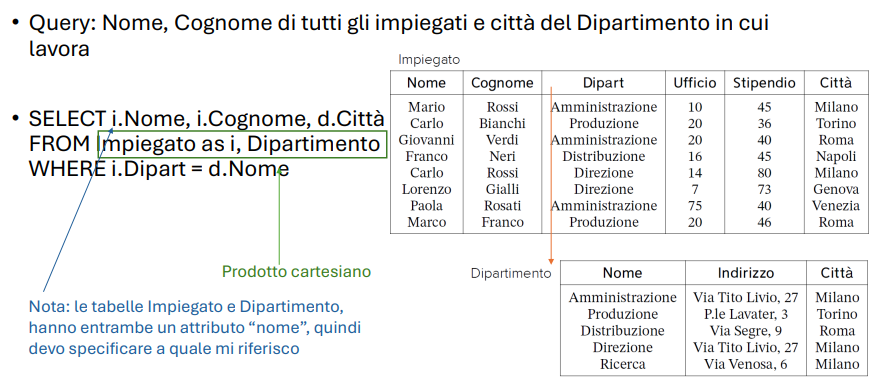
\includegraphics[width=1\linewidth]{image155}
	\caption{Esempio}
	\label{fig:image155}
\end{figure}
Il \textbf{join} può essere specificato direttamente nella clausola
\texttt{FROM}, a livello delle tabelle coinvolte. Nello svolgimento degli
esercizi utilizzeremo questa sintassi dedicata.

\begin{verbatim}
	SELECT ListaAttributi
	FROM Tabella1 JOIN Tabella2 ON (CondizioneDiJoin)
	[WHERE AltraCondizione]
\end{verbatim}

Esempio:

\begin{verbatim}
	SELECT i.Nome, d.Città
	FROM Impiegato AS i JOIN Dipartimento AS d
	ON (i.Dipart = d.Nome)
\end{verbatim}
\textbf{Q8:} Selezionare i padri di persone che guadagnano più di 20.

\medskip

\textbf{Algebra relazionale}

\[
\pi_{Padre} \big( \text{Paternità} \ \bowtie_{Figlio = Nome} \ (\sigma_{Reddito > 20}(\text{Persone})) \big)
\]

\medskip

\textbf{SQL}

\begin{verbatim}
	SELECT DISTINCT Padre
	FROM Persone
	JOIN Paternità ON (Figlio = Nome)
	WHERE Reddito > 20;
\end{verbatim}
\subsection{Uso di variabili (alias)}

SQL permette di associare un \textbf{nome alternativo} (alias) alle tabelle
che compaiono nella clausola \texttt{FROM}.

\begin{itemize}
	\item Il nome alternativo viene utilizzato per fare riferimento alla
	tabella nel contesto dell'interrogazione.
	
	\item L'alias viene definito nella clausola \texttt{FROM} tramite la
	parola chiave \texttt{AS} (opzionale).
\end{itemize}

\textbf{Motivi per usare gli alias:}

\begin{itemize}
	\item Fare riferimento alla tabella in modo più compatto.
	\item Accedere più volte alla stessa tabella all'interno della stessa
	interrogazione (self join).
\end{itemize}
\begin{figure}[H]
	\centering
	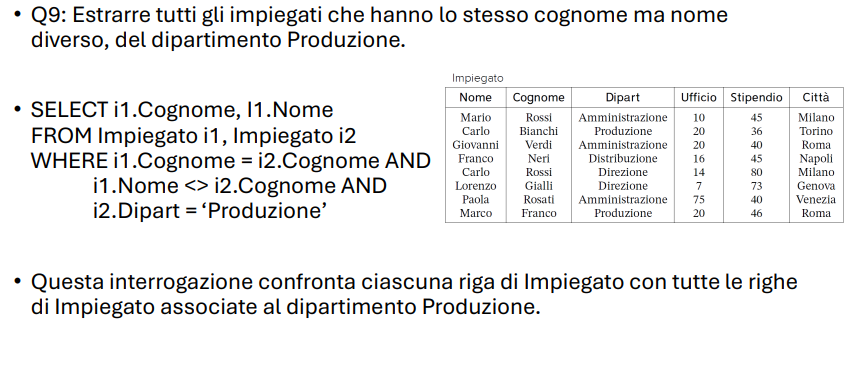
\includegraphics[width=1\linewidth]{image156}
	\caption{Esempio Uso di variabili (alias)}
	\label{fig:image156}
\end{figure}
\begin{itemize}
	\item Si può immaginare che, al momento della definizione degli alias,
	vengano create due copie della tabella \texttt{Impiegato}, ciascuna
	associata a una delle due variabili \texttt{i1} e \texttt{i2}.
	
	\item Le due copie contengono inizialmente tutte le righe della tabella
	\texttt{Impiegato}.
	
	\item Successivamente, sulla copia \texttt{i2} vengono selezionate solo
	le righe relative al dipartimento \texttt{'Produzione'}.
\end{itemize}
\subsection{Ordinamento del risultato}
Come abbiamo visto, una relazione è un insieme di tuple \textbf{non ordinato}.
Nella pratica, però, spesso è necessario visualizzare le righe secondo
un determinato ordine.

SQL permette di specificare un ordinamento (ascendente o discendente)
delle righe dell'output tramite la clausola \texttt{ORDER BY}, che viene
posta alla fine dell'interrogazione.
\begin{figure}[H]
	\centering
	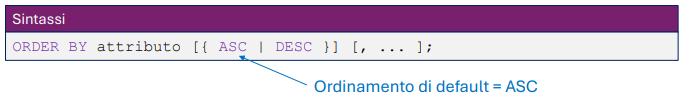
\includegraphics[width=1\linewidth]{image157}
	\caption{Sintassi Ordinamento del risultato}
	\label{fig:image157}
\end{figure}
Se nella clausola \texttt{ORDER BY} sono presenti più attributi, le righe
vengono ordinate rispetto al primo attributo dell'elenco; a parità di valore
del primo attributo si utilizza il secondo, e così via in sequenza.
\begin{figure}[H]
	\centering
	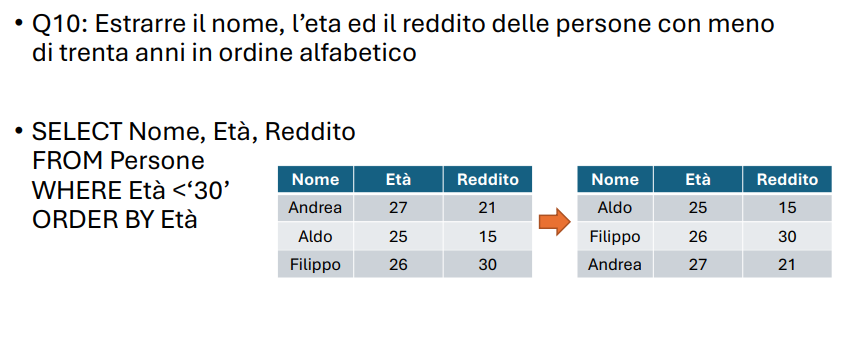
\includegraphics[width=1\linewidth]{image158}
	\caption{Esempio: Ordinamento del risultato}
	\label{fig:image158}
\end{figure}
\begin{figure}[H]
	\centering
	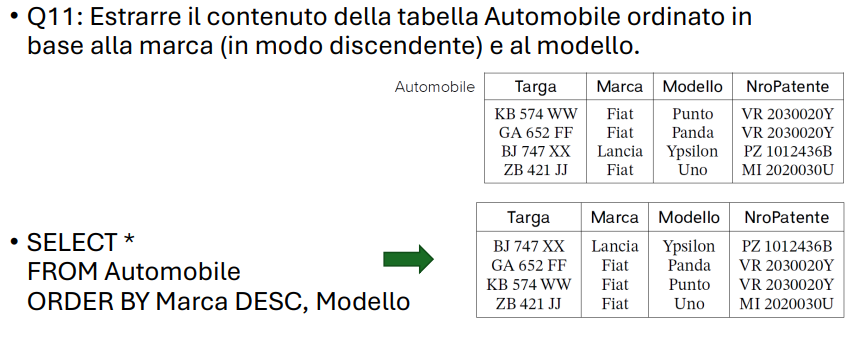
\includegraphics[width=1\linewidth]{image159}
	\caption{Esempio Ordinamento del risultato}
	\label{fig:image159}
\end{figure}
\subsubsection{Operazioni Insiemistiche}
SQL mette a disposizione alcuni \textbf{operatori insiemistici} che permettono
di combinare i risultati di più interrogazioni.

\begin{verbatim}
	SELECT ...
	{ UNION | INTERSECT | EXCEPT [ALL] }
	SELECT ...
\end{verbatim}

\begin{itemize}
	\item Gli operatori insiemistici, a differenza del resto del linguaggio SQL,
	\textbf{eliminano i duplicati per default}. 
	
	\item Se si vogliono mantenere i duplicati è necessario utilizzare la
	parola chiave \texttt{ALL}.
	
	\item Le interrogazioni combinate devono restituire lo stesso
	\textbf{numero di attributi} e avere \textbf{domini compatibili}.
	
	\item La corrispondenza tra gli attributi avviene per \textbf{posizione}
	(ordine posizionale), non per nome.
	
	\item Se i nomi degli attributi sono diversi, di solito il sistema utilizza
	il nome degli attributi del \textbf{primo operando}.
\end{itemize}
\subsubsection{Unione}
\begin{figure}[H]
	\centering
	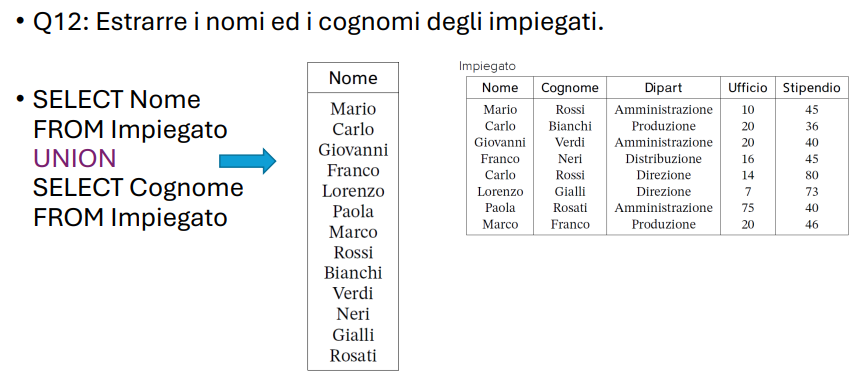
\includegraphics[width=1\linewidth]{image160}
	\caption{Esempio Unione}
	\label{fig:image160}
\end{figure}
\begin{figure}[H]
	\centering
	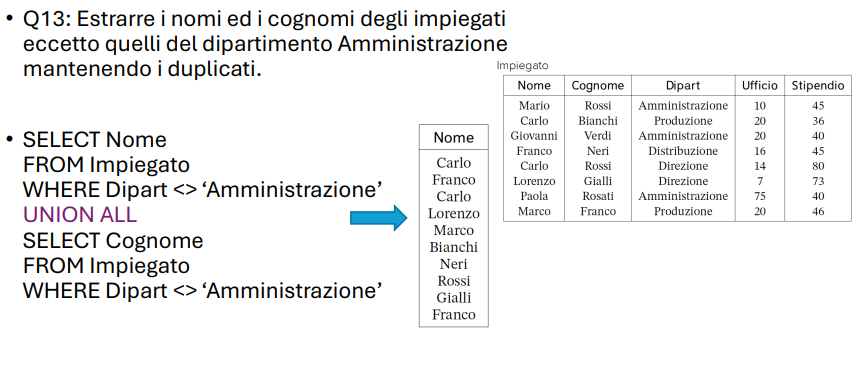
\includegraphics[width=1\linewidth]{image161}
	\caption{Esempio Unione}
	\label{fig:image161}
\end{figure}
\subsubsection{Intersezione}
\begin{figure}[H]
	\centering
	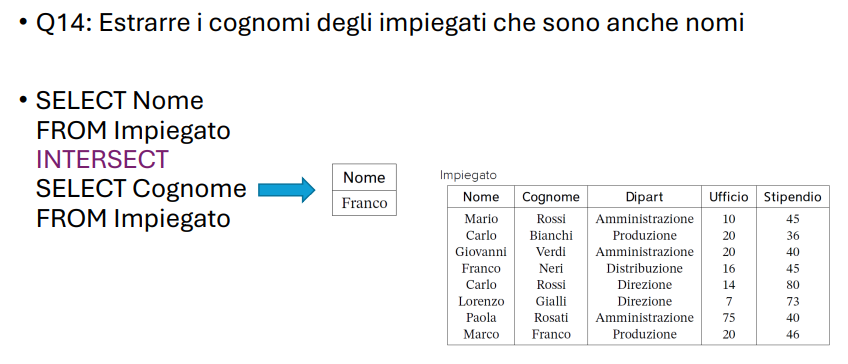
\includegraphics[width=1\linewidth]{image162}
	\caption{Intersezione}
	\label{fig:image162}
\end{figure}
\subsubsection{Differenza}
\begin{figure}[H]
	\centering
	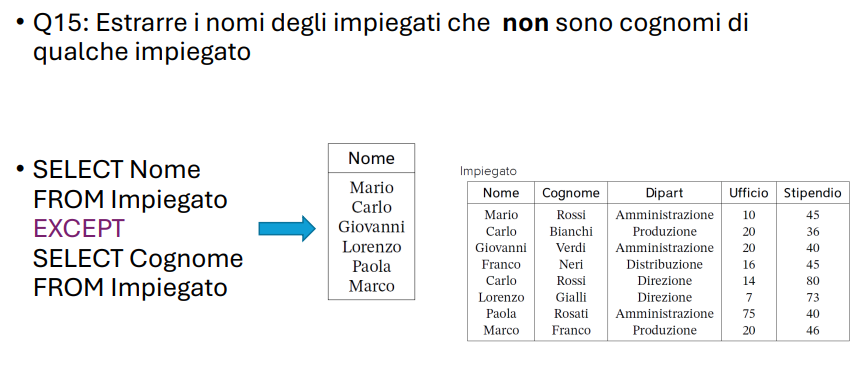
\includegraphics[width=1\linewidth]{image163}
	\caption{Differenza}
	\label{fig:image163}
\end{figure}
\subsection{Operatori aggregati}

Gli operatori di aggregazione rappresentano una delle più importanti
estensioni di SQL rispetto all'algebra relazionale.

\begin{itemize}
	\item I principali operatori di aggregazione sono:
	\texttt{COUNT}, \texttt{SUM}, \texttt{MAX}, \texttt{MIN} e \texttt{AVG}.
	
	\item Nell'algebra relazionale tutte le condizioni specificate vengono
	valutate su \textbf{una tupla alla volta}.
	
	\item Gli operatori di aggregazione, invece, permettono di valutare
	proprietà che dipendono da \textbf{insiemi di tuple}.
	
	\item Prima viene eseguita l'interrogazione considerando solo le
	clausole \texttt{FROM} e \texttt{WHERE}.
	
	\item Successivamente l'operatore di aggregazione viene applicato
	alla tabella contenente il risultato dell'interrogazione.
\end{itemize}
\subsubsection{COUNT}
L'operatore \texttt{COUNT} conta il numero di righe di una tabella oppure
il numero di valori di uno o più attributi.

\begin{verbatim}
	COUNT ( <* | [DISTINCT | ALL] ListaAttributi> )
\end{verbatim}

\begin{itemize}
	\item \texttt{*}: conta il numero totale di righe della tabella.
	
	\item \texttt{DISTINCT ListaAttributi}: conta il numero di valori
	\textbf{distinti} degli attributi specificati.
	
	\item \texttt{ALL ListaAttributi}: conta il numero di righe che hanno
	valori \textbf{diversi da NULL} negli attributi indicati.
	
	\item \texttt{ALL} rappresenta il \textbf{comportamento di default}.
\end{itemize}
\begin{figure}[H]
	\centering
	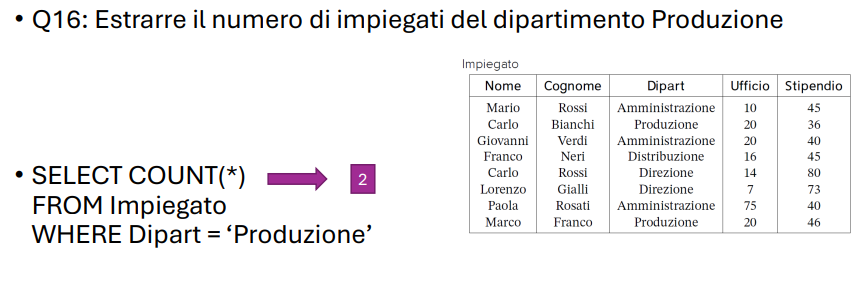
\includegraphics[width=1\linewidth]{image164}
	\caption{Esempio COUNT}
	\label{fig:image164}
\end{figure}
\begin{figure}[H]
	\centering
	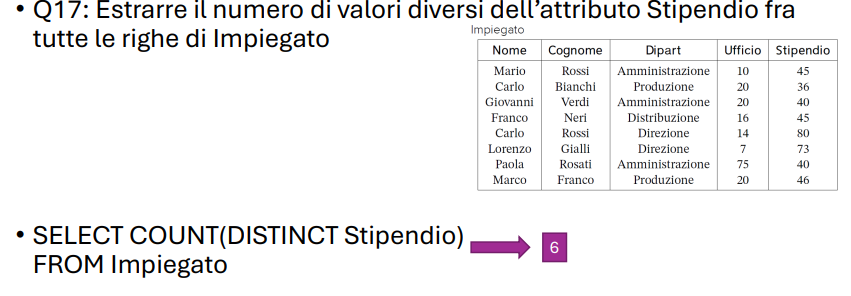
\includegraphics[width=1\linewidth]{image165}
	\caption{Esempio Count}
	\label{fig:image165}
\end{figure}
\begin{figure}[H]
	\centering
	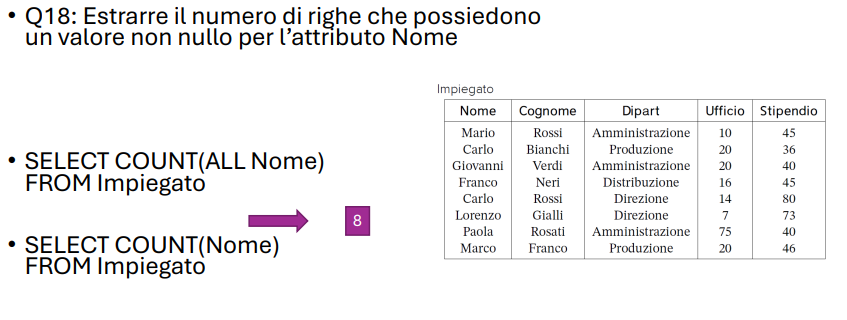
\includegraphics[width=1\linewidth]{image166}
	\caption{Esempio Count}
	\label{fig:image166}
\end{figure}
\subsubsection{Operatori aggregati: SUM.MAX,MIN,AVG}
\begin{verbatim}
	<SUM | MAX | MIN | AVG> ( [DISTINCT | ALL] AttrExpr )
\end{verbatim}

\begin{itemize}
	\item \texttt{SUM}: restituisce la somma dei valori posseduti
	dall'espressione.
	
	\item \texttt{MAX} / \texttt{MIN}: restituiscono rispettivamente il
	valore massimo o minimo tra quelli posseduti dall'espressione.
	
	\item \texttt{AVG}: restituisce la media dei valori.
	
	\item \texttt{SUM} e \texttt{AVG} ammettono come argomento solo
	espressioni che rappresentano valori \textbf{numerici} o
	\textbf{intervalli di tempo}.
	
	\item \texttt{MAX} e \texttt{MIN} ammettono come argomento
	espressioni su cui è definito un \textbf{ordinamento}
	(ad esempio anche stringhe).
	
	\item \texttt{DISTINCT} elimina i valori duplicati prima
	dell'applicazione dell'operatore.
	
	\item \texttt{ALL} considera tutti i valori, \textbf{trascurando solo
		i valori NULL}. Questo è il comportamento di default.
	
	\item \texttt{DISTINCT} e \texttt{ALL} non hanno effetto sugli
	operatori \texttt{MIN} e \texttt{MAX}.
\end{itemize}
\begin{figure}[H]
	\centering
	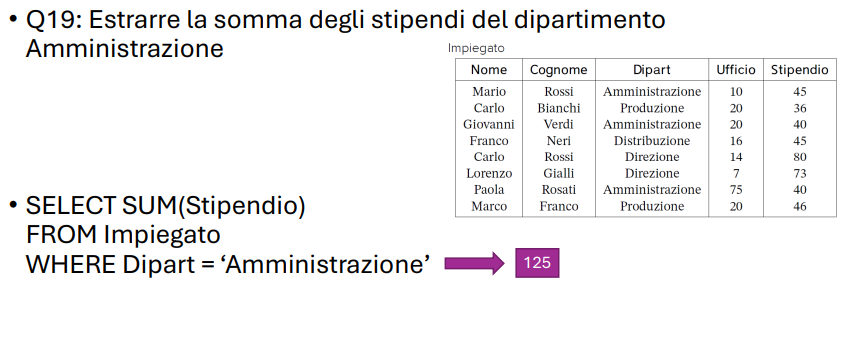
\includegraphics[width=1\linewidth]{image167}
	\caption{Esempio SUM}
	\label{fig:image167}
\end{figure}
\begin{figure}[H]
	\centering
	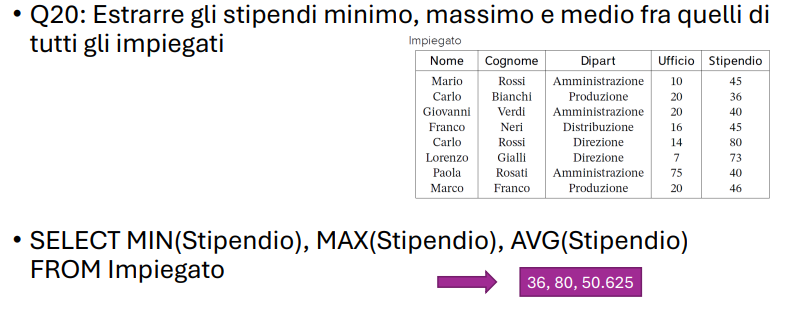
\includegraphics[width=1\linewidth]{image168}
	\caption{Esempio MAX,MIN,AVG}
	\label{fig:image168}
\end{figure}
\begin{figure}[H]
	\centering
	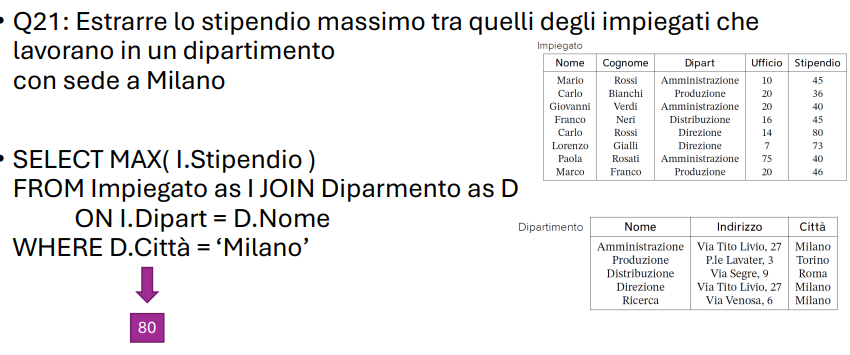
\includegraphics[width=1\linewidth]{image169}
	\caption{Esempio MAX}
	\label{fig:image169}
\end{figure}
\begin{verbatim}
	SELECT Cognome, Nome, MAX(I.Stipendio)
	FROM Impiegato AS I JOIN Dipartimento AS D
	ON I.Dipart = D.Nome
	WHERE D.Città = 'Milano'
\end{verbatim}

\begin{itemize}
	\item La seguente interrogazione non è corretta.
	
	\item Gli operatori di aggregazione non sono un meccanismo di selezione,
	ma funzioni che restituiscono un valore quando vengono applicate
	a un insieme di tuple.
	
	\item Gli attributi \texttt{Cognome} e \texttt{Nome} restituiscono
	un valore per \textbf{ogni tupla selezionata}, mentre
	\texttt{MAX()} restituisce un \textbf{unico valore} per
	l'intero insieme.
	
	\item Si crea quindi un'incoerenza tra attributi normali
	e funzione di aggregazione.
	
	\item Per risolvere questa situazione è necessario utilizzare
	il meccanismo di \textbf{raggruppamento} tramite la clausola
	\texttt{GROUP BY}.
\end{itemize}
\subsection{Interrogazioni con raggruppamento}
Gli operatori di aggregazione possono essere applicati separatamente
a \textbf{sottoinsiemi di righe}.

\begin{itemize}
	\item La clausola \texttt{GROUP BY} permette di specificare come
	dividere le righe della tabella in sottoinsiemi.
	
	\item La clausola consente di indicare un insieme di attributi
	rispetto ai quali effettuare il raggruppamento.
	
	\item L'interrogazione raggruppa quindi tutte le righe che
	possiedono gli \textbf{stessi valori} per tali attributi.
\end{itemize}
\begin{figure}[H]
	\centering
	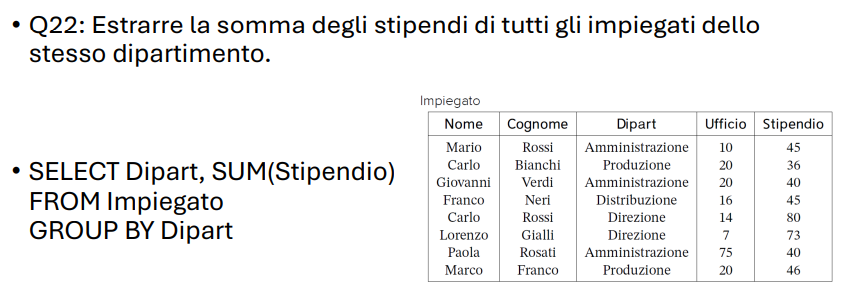
\includegraphics[width=1\linewidth]{image170}
	\caption{Esempio GROUP BY}
	\label{fig:image170}
\end{figure}
\begin{figure}[H]
	\centering
	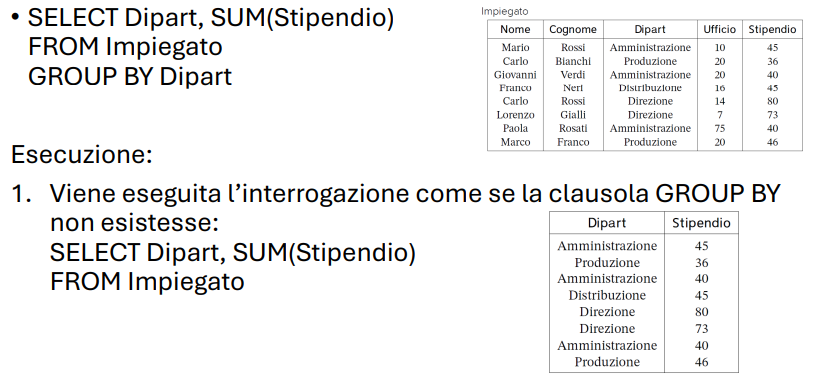
\includegraphics[width=1\linewidth]{image171}
	\caption{Esempio GROUP BY}
	\label{fig:image171}
\end{figure}
\begin{figure}[H]
	\centering
	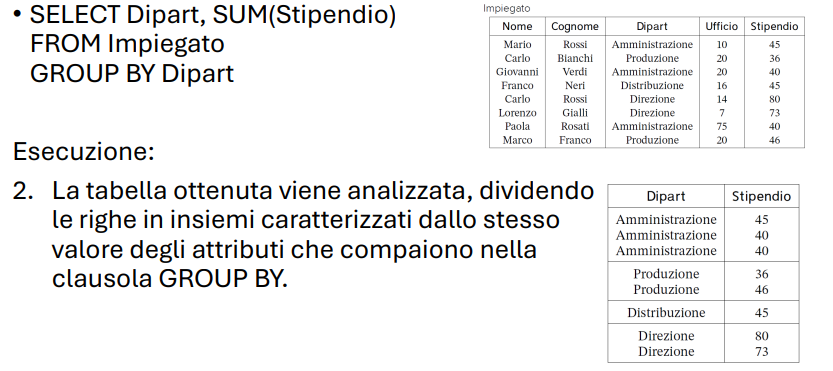
\includegraphics[width=1\linewidth]{image172}
	\caption{Esempio GROUP BY}
	\label{fig:image172}
\end{figure}
\begin{figure}[H]
	\centering
	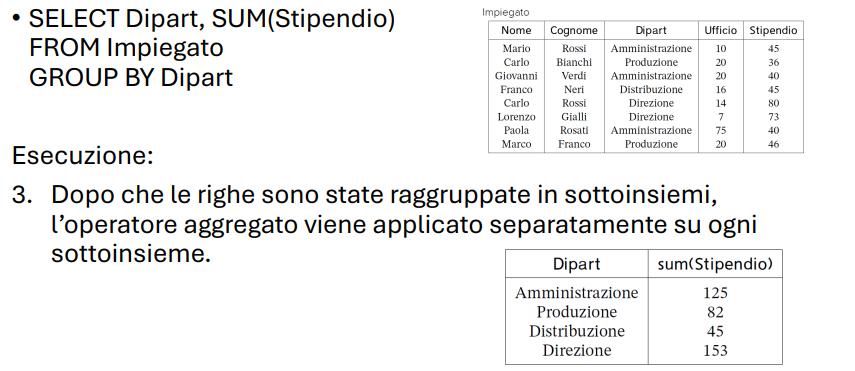
\includegraphics[width=1\linewidth]{image173}
	\caption{Esempio GROUP BY}
	\label{fig:image173}
\end{figure}
In una interrogazione che utilizza la clausola \texttt{GROUP BY}, nella
clausola \texttt{SELECT} possono comparire solo:

\begin{itemize}
	\item attributi che appartengono all'insieme specificato nella
	clausola \texttt{GROUP BY};
	\item oppure operatori di aggregazione.
\end{itemize}

\textbf{Esempio di interrogazione non corretta}

\begin{verbatim}
	SELECT Ufficio
	FROM Impiegato
	GROUP BY Dipart
\end{verbatim}

\textbf{Errore:}

\begin{itemize}
	\item Ad ogni valore dell'attributo \texttt{Dipart} possono
	corrispondere diversi valori dell'attributo \texttt{Ufficio}.
	
	\item Ogni sottoinsieme di righe generato dal \texttt{GROUP BY}
	deve corrispondere ad \textbf{una sola riga} nella tabella
	risultato.
\end{itemize}
\subsubsection{HAVING}
È possibile applicare delle \textbf{selezioni ai gruppi} generati tramite
la clausola \texttt{GROUP BY}.

\begin{itemize}
	\item La clausola \texttt{HAVING} permette di specificare condizioni
	che devono essere soddisfatte dai \textbf{gruppi di tuple} generati
	dopo l'esecuzione del raggruppamento tramite \texttt{GROUP BY}.
	
	\item A differenza della clausola \texttt{WHERE}, che filtra le
	\textbf{singole tuple} prima del raggruppamento, la clausola
	\texttt{HAVING} filtra i \textbf{gruppi} dopo il raggruppamento.
\end{itemize}

\textbf{Esempio}

\begin{verbatim}
	SELECT Dipart, SUM(Stipendio) AS SommaStipendi
	FROM Impiegato
	GROUP BY Dipart
	HAVING SUM(Stipendio) > 100;
\end{verbatim}
\begin{figure}[H]
	\centering
	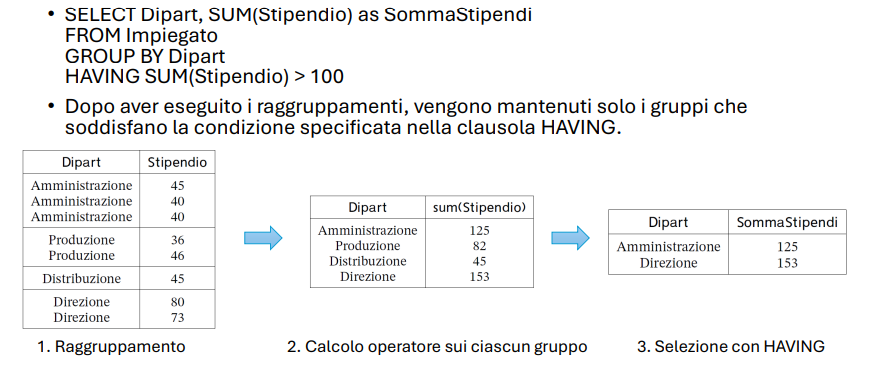
\includegraphics[width=1\linewidth]{image174}
	\caption{HAVING + GROUP BY}
	\label{fig:image174}
\end{figure}
\begin{itemize}
	\item La clausola \texttt{WHERE} applica delle selezioni su
	\textbf{singole righe}, prima dell'eventuale raggruppamento
	tramite \texttt{GROUP BY}.
	
	\item La clausola \texttt{HAVING} applica delle selezioni su
	\textbf{gruppi di righe}, generati dopo l'esecuzione del
	raggruppamento tramite \texttt{GROUP BY}.
\end{itemize}

\textbf{Esempio}

\begin{verbatim}
	SELECT Dipart
	FROM Impiegato
	WHERE Ufficio = 20
	GROUP BY Dipart
	HAVING AVG(Stipendio) > 25;
\end{verbatim}

\textbf{Ordine logico di esecuzione}

\begin{enumerate}
	\item \texttt{WHERE} → seleziona le righe che verranno raggruppate.
	\item \texttt{GROUP BY} → forma i gruppi con le righe selezionate.
	\item \texttt{HAVING} → seleziona i gruppi che faranno parte del risultato.
\end{enumerate}
\subsection{Interrogazioni nidificate}
Una \textbf{interrogazione nidificata} è una interrogazione SQL che
contiene al suo interno una o più interrogazioni.

\begin{itemize}
	\item La nidificazione può avvenire nella clausola \texttt{SELECT},
	nella clausola \texttt{FROM} oppure nella clausola \texttt{WHERE}.
	
	\item Il caso più comune è la nidificazione nella clausola
	\texttt{WHERE}.
	
	\item In questo caso un predicato contiene un confronto tra
	un valore (un'espressione valutata su una singola riga) e
	il risultato di un'altra interrogazione SQL.
\end{itemize}
Quando in un predicato si confronta un attributo (o un'espressione che
produce un valore singolo) con il risultato di un'interrogazione,
può sorgere un problema di disomogeneità tra i termini del confronto,
poiché la sottointerrogazione può restituire più valori.

\begin{itemize}
	\item I normali operatori di confronto
	(\texttt{=}, \texttt{<>}, \texttt{<}, \texttt{>}, \texttt{<=}, \texttt{>=})
	possono essere estesi con le parole chiave \texttt{ANY} e \texttt{ALL}.
	
	\item \texttt{ANY}: la riga soddisfa la condizione se il confronto
	tra il valore dell'attributo (o dell'espressione) e \textbf{almeno
		uno} dei valori restituiti dalla sottointerrogazione risulta vero.
	
	\item \texttt{ALL}: la riga soddisfa la condizione se il confronto
	tra il valore dell'attributo (o dell'espressione) e \textbf{tutti}
	i valori restituiti dalla sottointerrogazione risulta vero.
\end{itemize}
\begin{figure}[H]
	\centering
	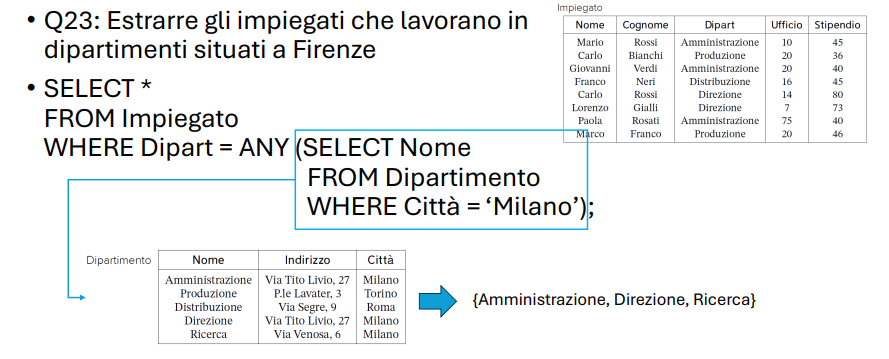
\includegraphics[width=1\linewidth]{image175}
	\caption{WHERE}
	\label{fig:image175}
\end{figure}
\begin{figure}[H]
	\centering
	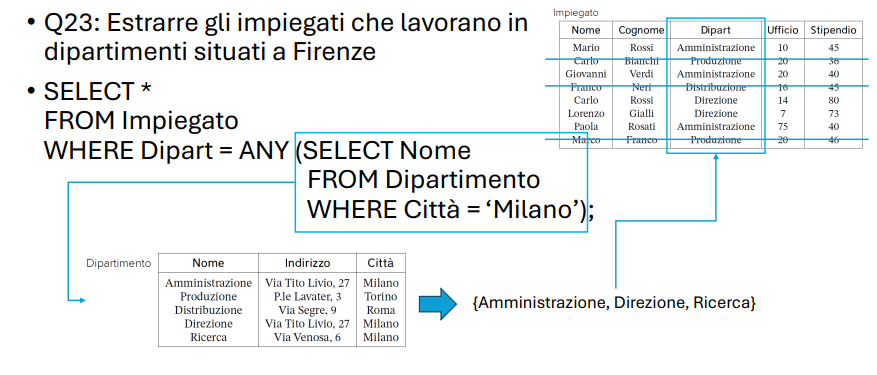
\includegraphics[width=1\linewidth]{image176}
	\caption{}
	\label{fig:image176}
\end{figure}
\begin{figure}[H]
	\centering
	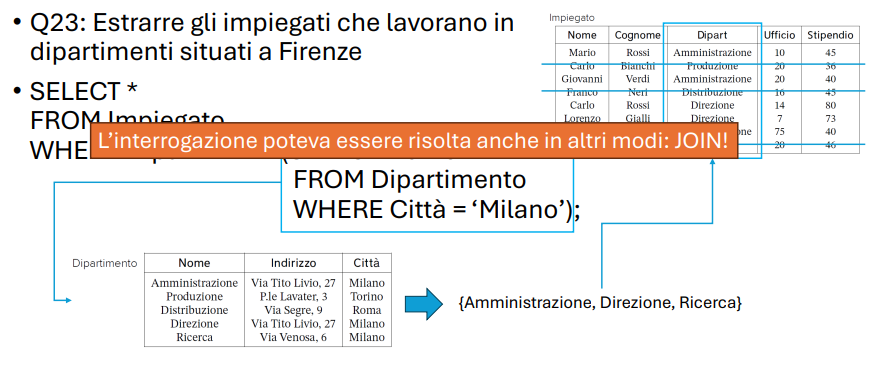
\includegraphics[width=1\linewidth]{image177}
	\caption{}
	\label{fig:image177}
\end{figure}
\begin{figure}[H]
	\centering
	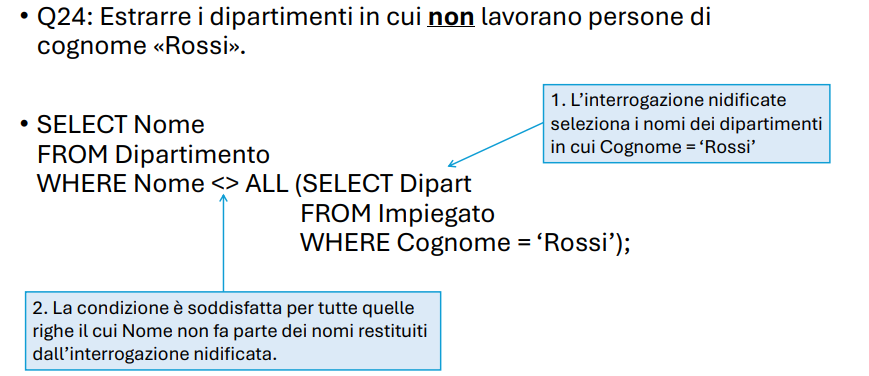
\includegraphics[width=1\linewidth]{image178}
	\caption{}
	\label{fig:image178}
\end{figure}
\textbf{Esempio con ALL}

\begin{verbatim}
	SELECT Nome
	FROM Dipartimento
	WHERE Nome <> ALL
	(SELECT Dipart
	FROM Impiegato
	WHERE Cognome = 'Rossi');
\end{verbatim}

Questa interrogazione seleziona i dipartimenti il cui nome è
\textbf{diverso da tutti} i valori restituiti dalla sottointerrogazione,
cioè i dipartimenti in cui non lavora nessun impiegato con cognome
\texttt{'Rossi'}.

\medskip

\textbf{Interrogazione equivalente}

\begin{verbatim}
	SELECT Nome
	FROM Dipartimento
	EXCEPT
	SELECT Dipart
	FROM Impiegato
	WHERE Cognome = 'Rossi';
\end{verbatim}
Per le interrogazioni nidificate viste fino ad ora, la sottointerrogazione
può essere eseguita \textbf{una sola volta} e il risultato ottenuto può
essere salvato in una \textbf{tabella temporanea}, utilizzata per
eseguire i confronti con le righe della tabella esterna.

\begin{itemize}
	\item In alcuni casi, però, la sottointerrogazione fa riferimento
	al contesto dell'interrogazione esterna tramite l'uso di una
	variabile (passaggio di \textit{binding}).
	
	\item In questo caso si parla di \textbf{interrogazione nidificata
		correlata}.
	
	\item La sottointerrogazione deve essere quindi valutata
	\textbf{separatamente per ogni riga} prodotta
	dall'interrogazione esterna.
\end{itemize}
L'operatore logico \texttt{EXISTS} riceve come parametro
un'interrogazione nidificata e restituisce il valore \textbf{vero}
solo se la sottointerrogazione produce un risultato \textbf{non vuoto}.

\begin{itemize}
	\item Se la sottointerrogazione restituisce almeno una riga,
	la condizione \texttt{EXISTS} risulta vera.
	
	\item Se la sottointerrogazione non restituisce alcuna riga,
	la condizione \texttt{EXISTS} risulta falsa.
	
	\item Questo operatore è particolarmente utile quando esiste
	un \textbf{passaggio di binding} tra la query esterna e la
	sottointerrogazione.
\end{itemize}
\begin{figure}[H]
	\centering
	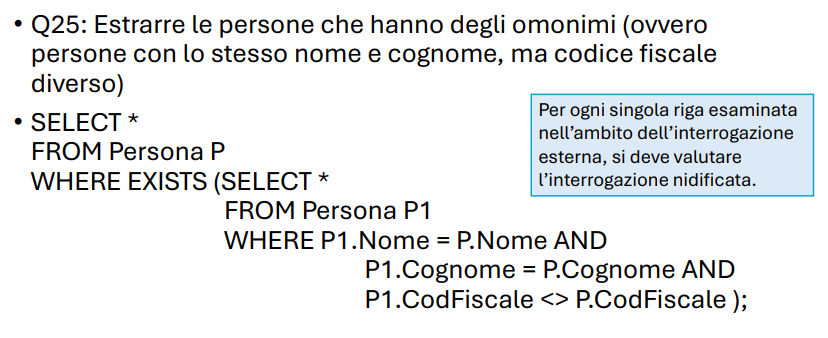
\includegraphics[width=1\linewidth]{image179}
	\caption{}
	\label{fig:image179}
\end{figure}
\begin{figure}[H]
	\centering
	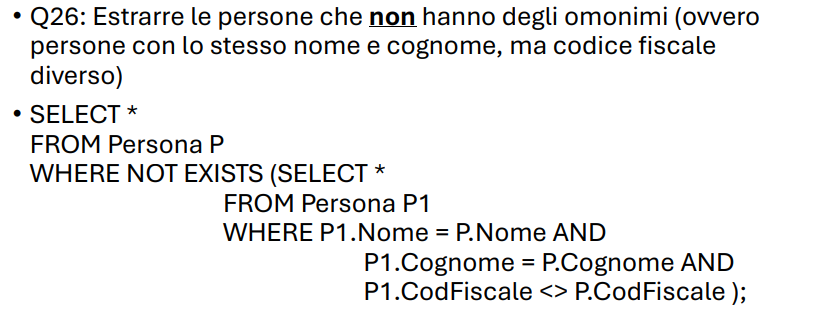
\includegraphics[width=1\linewidth]{image180}
	\caption{}
	\label{fig:image180}
\end{figure}
\begin{figure}[H]
	\centering
	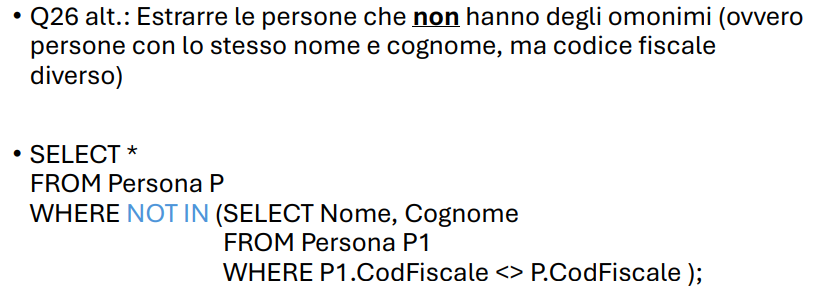
\includegraphics[width=1\linewidth]{image181}
	\caption{}
	\label{fig:image181}
\end{figure}
\begin{figure}[H]
	\centering
	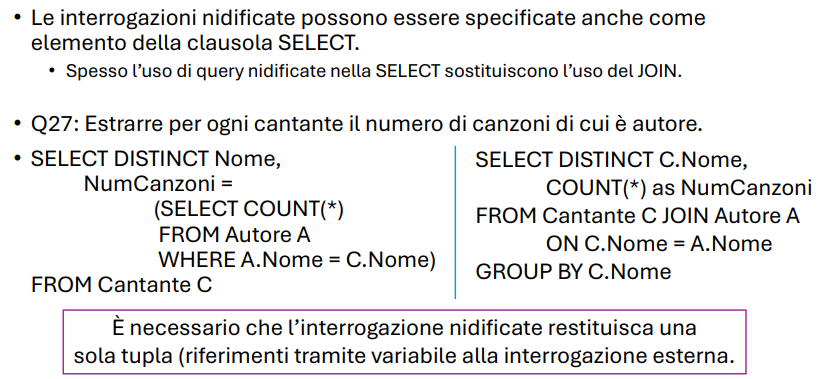
\includegraphics[width=1\linewidth]{image182}
	\caption{}
	\label{fig:image182}
\end{figure}
Le interrogazioni nidificate possono essere utilizzate nella
clausola \texttt{FROM} come sorgenti di dati su cui eseguire
l'interrogazione principale.

\begin{itemize}
	\item È possibile creare una \textbf{catena di interrogazioni},
	in cui ogni interrogazione utilizza il risultato della
	precedente come se fosse una tabella di base.
	
	\item In questo modo il risultato di una sottointerrogazione
	viene trattato come una \textbf{tabella temporanea}.
\end{itemize}

\textbf{Q28:} Estrarre per ogni cantante che è anche autore di canzoni
il numero di canzoni di cui è rispettivamente interprete e autore.

\begin{verbatim}
	SELECT DISTINCT C.Nome, C.NumCantate, A.NumScritte
	FROM
	(SELECT Nome, COUNT(*) AS NumCantate
	FROM Cantante
	GROUP BY Nome) C
	JOIN
	(SELECT Nome, COUNT(*) AS NumScritte
	FROM Autore
	GROUP BY Nome) A
	ON C.Nome = A.Nome;
\end{verbatim}

\begin{itemize}
	\item Prima vengono eseguite le interrogazioni presenti nella
	clausola \texttt{FROM}.
	
	\item I risultati ottenuti vengono poi utilizzati come
	\textbf{normali tabelle} nell'interrogazione esterna.
\end{itemize}
	
\end{document}